\documentclass[a4paper, 12pt, openany]{book} %chose the paper size and font size. Openany ensures that all all chapters and similar may begin at any page, not only odd pages. For the introductory pages and appendices we want openany, but for chapter pages in the main content we want chapters to begin only on odd pages (right hand side). The book class ensures that the margins are automatically adjusted such that left hand pages are slightly moved to the left and vice versa at the right, which makes the thesis very readable and good looking when printed in bound book format.
%\usepackage{titlesec}
%\titlespacing*{\chapter}{0pt}{-20pt}{20pt}
\usepackage[utf8]{inputenc} %to manage special characters
\usepackage[hidelinks]{hyperref}
\usepackage[T1]{fontenc} %to manage special characters
\usepackage[Sonny]{fncychap} %fancy chapter style (many more available, like Sonny or Lenny etc.)
\usepackage{fancyhdr}
\usepackage{subcaption}%to customize the headers
\usepackage[lmargin=1.5in, rmargin=1in, tmargin=1in, bmargin=1in]{geometry} %sets the margins for the pages
\setcounter{tocdepth}{3} %table of contents number depth for subsections (2 = x.x.x)
\setcounter{secnumdepth}{4} %numbering depth for headers for subsections in the text(4 = x.x.x.x)
\usepackage{url} %to include urls
\usepackage{listings} %include this if you want to include code in the thesis
\usepackage{amsmath,amssymb} %mathematical package
\usepackage{siunitx} %includes SI-units
\usepackage[bf]{caption} %makes float captions bold
\usepackage{array, booktabs} %to make better tables
\usepackage{graphicx} %to include graphics
\usepackage{float} %to include floats
\usepackage[export]{adjustbox} %to adjust floats
\usepackage{subfig} %to include subfigures
\usepackage{chngcntr} %will make it possible to change the counter for tables, figures etc. such as below
\usepackage{gensymb}
\counterwithin{figure}{section} %change counter for figures within sections (also possible to choose for each chapter
\usepackage{tikz}
\usetikzlibrary{arrows.meta, positioning}
\counterwithin{table}{section} %change counter for tables within sections
\usepackage{color, xcolor} %edit e.g. text colors
\usepackage{listings}
\usepackage{xcolor}
\usepackage{hyperref}
\definecolor{codegray}{gray}{0.45}
\definecolor{codepurple}{rgb}{0.45,0.15,0.55}
\definecolor{codegreen}{rgb}{0.0,0.45,0.0}
\definecolor{backgray}{rgb}{0.97,0.97,0.97}



\lstdefinestyle{basecode}{
    backgroundcolor=\color{backgray},
    basicstyle=\ttfamily\scriptsize,
    numbers=left,
    numberstyle=\tiny\color{codegray},
    stepnumber=1,
    numbersep=8pt,
    frame=single,
    rulecolor=\color{black},
    breaklines=true,
    breakatwhitespace=false,
    columns=fullflexible,
    keepspaces=true,
    showstringspaces=false,
    tabsize=4,
    captionpos=b,
    xleftmargin=1.5em,
    framexleftmargin=1em,
    linewidth=\linewidth
}

\lstdefinestyle{cstyle}{
    style=basecode,
    language=C,
    keywordstyle=\color{blue},
    commentstyle=\color{codegreen},
    stringstyle=\color{codepurple}
}

\lstdefinestyle{cppstyle}{
    style=basecode,
    language=C++,
    keywordstyle=\color{blue},
    commentstyle=\color{codegreen},
    stringstyle=\color{codepurple}
}

\lstdefinestyle{pythonstyle}{
    style=basecode,
    language=Python,
    keywordstyle=\color{blue},
    commentstyle=\color{codegreen},
    stringstyle=\color{codepurple}
}
\usepackage[backend = biber,
            style = apa,
            date = long,     % Long: 24th Mar. 1997 | Short: 24/03/1997
            sorting = none,
            maxcitenames = 3,   % max names to include before et. al.
            ]{biblatex} %customize the look of your citations and bibliography
\addbibresource{bibliography.bib} %declare the bibliography resource
\usepackage{comment} %to be able to comment out sections in the .tex files
\usepackage{afterpage} %to customize page commands such as below
\newcommand\myemptypage{
    \null
    \thispagestyle{empty}
    \addtocounter{page}{-1}
    \newpage
    } %sets new page command to insert an empty page without adding to the page counter or having a page number




\begin{document}
%%%%%%%%%%%%%%%%%%%%%%%%%%%%%%%%%%%%%%%%%%%%%%%%%%%%%%%%
%\begin{comment}
% The title page:
% For NTNU students this page will be generated automatically when submitting your paper, and should not be included in the final file from Latex. Delete or comment out the title page setup. The final report should then start with the first page being the abstract. I have included a title page here so it is possible to see how it may look like, and for those who does not get an automatically generated title page. Of course you will need to change the names and titles etc. to your case.

%the title page should be an odd page (right hand side)
%%%%%%%%%%%%%%%%%%%%%%%%%%%%%%%%%%%%%%%%%%%%%%%%%%%%%%%%

% The pre-chapters
\chapter*{Abstract} %pre-chapters should not be numbered, hence the "*"
\pagenumbering{roman} %introductory pages should be roman
\setcounter{page}{1}
\addcontentsline{toc}{chapter}{\protect\numberline{}Abstract} %add the chapter to the table of contents, this is not automatically added when creating unnumbered chapters (*). Add it in a chapter style, and keep all chapters on the same numberline indent regardless of number or not on the chapter
The increasing accessibility and falling cost of consumer drones has 
created a growing need for affordable detection systems that can be 
deployed by private individuals and small organisations. Existing 
commercial solutions based on radar and electro-optical sensors are 
priced far beyond the reach of most non-military users, while 
academic research in this area rarely reports hardware costs alongside 
detection performance. This thesis presents the design, implementation, 
and testing of a low-cost multimodal drone detection system built 
entirely from off-the-shelf and 3D-printed components, with a total 
hardware cost of approximately NOK~ 10,000.

The system combines a four-element MEMS microphone array with a 
pan-tilt camera platform running a YOLOv8n object detection model, 
following a coarse-to-fine detection strategy in which acoustic 
direction of arrival estimation orients the camera toward the target 
before visual detection takes over. Acoustic signal acquisition is 
handled by an STM32F413 microcontroller using the DFSDM peripheral 
for PDM-to-PCM conversion, with direction of arrival estimated using 
the GCC-PHAT algorithm. Sound classification is performed by two 
machine learning models: a Convolutional Neural Network and a 
decision-tree classifier, both trained on a combination of public 
datasets and data collected with the microphone array. The YOLOv8n 
model was trained on a public drone detection dataset and deployed 
on a Raspberry Pi~5 with a Hailo AI HAT+ accelerator, achieving 
real-time inference at approximately 108 frames per second.

The acoustic DOA estimation was demonstrated to accurately track a 
live drone circulating around the tower in a laboratory environment, 
with a full detection pipeline iteration time of approximately 1.285 
seconds. The CNN sound classifier achieved 99\% accuracy on 
microphone array recordings and produced no false positives or 
negatives during the live test, while the YOLOv8n model achieved an 
mAP@0.50 of 0.835 and an F1 score of 0.81 on the validation dataset. 
Real-time visual detection and MQTT coordinate publishing were 
successfully demonstrated in a live laboratory test. The full 
closed-loop camera tracking was not completed within the project 
timeframe due to issues with the motor control hardware.

The results demonstrate that a capable multimodal drone detection 
system can be realised at a fraction of the cost of commercial 
alternatives, and provide a foundation for future development toward 
a complete autonomous detection and tracking platform.


\newpage
\textbf{Norsk sammendrag}

Den økte tilgjengeligheten og de fallende prisene på forbrukerdrones 
har skapt et voksende behov for rimelige deteksjonssystemer som kan 
tas i bruk av privatpersoner og mindre organisasjoner. Eksisterende 
kommersielle løsninger basert på radar og elektro-optiske sensorer er 
priset langt over det de fleste ikke-militære brukere har råd til, 
mens akademisk forskning på dette feltet sjelden rapporterer 
maskinvarekostnader sammen med deteksjonsytelse. Denne oppgaven 
presenterer design, implementasjon og testing av et lavkost multimodalt 
dronedeteksjonssystem bygget utelukkende av hyllevare- og 
3D-printede komponenter, med en total maskinvarekostnad på 
omtrent NOK~10,000.

Systemet kombinerer et firekanalers MEMS-mikrofonarrray med en 
pan-tilt-kameraplatform som kjører en YOLOv8n 
objektdeteksjonsmodell, etter en grov-til-fin deteksjonsstrategi 
der akustisk ankomsretningsestimering orienterer kameraet mot 
målet før visuell deteksjon overtar. Akustisk signalanskaffelse 
håndteres av en STM32F413-mikrokontroller ved hjelp av 
DFSDM-periferiutstyret for PDM-til-PCM-konvertering, med 
ankomsretning estimert ved hjelp av GCC-PHAT-algoritmen. 
Lydklassifisering utføres av to maskinlæringsmodeller: et 
konvolusjonelt nevralt nettverk og en beslutningstreklassifikator, 
begge trent på en kombinasjon av offentlige datasett og data samlet 
inn med mikrofonarrayen. YOLOv8n-modellen ble trent på et offentlig 
dronedeteksjonsdatasett og distribuert på en Raspberry Pi~5 med en 
Hailo AI HAT+-akselerator, og oppnådde sanntidsinferens med 
omtrent 108 bilder per sekund.

Den akustiske DOA-estimeringen ble demonstrert å nøyaktig spore en 
levende drone som sirkulerte rundt tårnet i et laboratoriumsmiljø, 
med en fullstendig deteksjonspipeline-iterasjonstid på omtrent 
1,285 sekunder. CNN-lydklassifikatoren oppnådde 99\% nøyaktighet 
på mikrofonarrayopptak og produserte ingen falske positiver eller 
negativer under livetesten, mens YOLOv8n-modellen oppnådde en 
mAP@0.50 på 0,835 og en F1-score på 0,81 på valideringsdatasettet. 
Sanntids visuell deteksjon og MQTT-koordinatpublisering ble 
vellykket demonstrert i en levende laboratorietest. Den fullstendige 
lukkede sløyfe-kamerasporing ble ikke fullført innenfor 
prosjekttidsrammen på grunn av problemer med motorstyringsmaskinvaren.

Resultatene viser at et kapabelt multimodalt dronedeteksjonssystem 
kan realiseres til en brøkdel av kostnadene for kommersielle 
alternativer, og gir et grunnlag for videre utvikling mot en 
komplett autonom deteksjons- og sporingsplattform.







 %insert the chapter text from the files

\chapter*{Preface}
\addcontentsline{toc}{chapter}{\protect\numberline{}Preface} 
%\noindent You may include acknowledgements and thanks as part of your preface on this page, or you may add it as a new chapter after the preface.

ChatGPT (\cite{chatgpt2026}) and Claude (\cite{anthropic2026}) were used as writing 
and programming aids throughout the project. All arguments, conclusions, 
and technical decisions presented in this thesis were identified and chosen 
independently by the authors. AI assistance was used solely to generate 
and/or refine the written formulation of these arguments, and all 
AI-assisted content was reviewed and verified by the authors before 
inclusion.

\tableofcontents
\addcontentsline{toc}{chapter}{\protect\numberline{}Contents}

%add to table of contents list of figures and tables, and insert list of figures and tables
\addcontentsline{toc}{chapter}{\protect\numberline{}\listfigurename}
\listoffigures
\addcontentsline{toc}{chapter}{\protect\numberline{}\listtablename}
\listoftables


\chapter*{Abbreviations}
\addcontentsline{toc}{chapter}{\protect\numberline{}Abbreviations}
% Put in your abbreviations here

List of all abbreviations:

% % \begin{itemize}
%     \item \textbf{PDM} Pulse Density Modulation
%     \item \textbf{PCM} Pulse Code Modulation
%     \item \textbf{MEMS} Micro Electrco Mechanical Systems 
%     \item \textbf{SNR} Signal to Noise Ratio 
%     \item \textbf{DFSDM} Digital filter sigma delta modulator
%     \item \textbf{Fs} Sampling frequency 
%     \item \textbf{MCU} Micro Controler Unit 
%     \item \textbf{DF} Digital Filter
%     \item \textbf{Std} Standard deviation
%     \item \textbf{UI} User interface
%     \item \textbf{DOA} Direction of Arrival
%     \item \textbf{ESD} Electrostatic Discharge
%     \item \textbf{RMS} Root Mean Square 
%     \item \textbf{EMI} Electromagnetic Interference 
%     \item \textbf{CNN} Convolutional neural network

% \end{itemize}

\begin{itemize}
    \item \textbf{AI} Artificial Intelligence
    \item \textbf{CDC} Communications Device Class
    \item \textbf{CNN} Convolutional Neural Network
    \item \textbf{CPS} Cross-Power Spectrum
    \item \textbf{CPU} Central Processing Unit
    \item \textbf{DC} Direct Current
    \item \textbf{DFC} Hailo Dataflow Compiler
    \item \textbf{DF} Digital Filter
    \item \textbf{DFSDM} Digital Filter Sigma-Delta Modulator
    \item \textbf{DFT} Discrete Fourier Transform
    \item \textbf{DFL} Distribution Focal Loss
    \item \textbf{DMA} Direct Memory Access
    \item \textbf{DOA} Direction of Arrival
    \item \textbf{EMI} Electromagnetic Interference
    \item \textbf{ESD} Electrostatic Discharge
    \item \textbf{FFT} Fast Fourier Transform
    \item \textbf{FOSR} Filter Oversampling Ratio
    \item \textbf{FPS} Frames Per Second
    \item \textbf{Fs} Sampling Frequency
    \item \textbf{GCC} Generalized Cross-Correlation
    \item \textbf{GPS} Global Positioning System
    \item \textbf{GPU} Graphics Processing Unit
    \item \textbf{GUI} Graphical User Interface
    \item \textbf{HAR} Hailo Archive
    \item \textbf{HEF} Hailo Executable Format
    \item \textbf{IDFT} Inverse Discrete Fourier Transform
    \item \textbf{IOSR} Integrator Oversampling Ratio
    \item \textbf{MCU} Microcontroller Unit
    \item \textbf{MEMS} Micro Electromechanical Systems
    \item \textbf{MFCC} Mel-Frequency Cepstral Coefficients
    \item \textbf{MLB} Mel Filter Bank
    \item \textbf{ML} Machine Learning
    \item \textbf{MQTT} Message Queue Telemetry Transport
    \item \textbf{ONNX} Open Neural Network Exchange
    \item \textbf{PCB} Printed Circuit Board
    \item \textbf{PCM} Pulse Code Modulation
    \item \textbf{PDM} Pulse Density Modulation
    \item \textbf{PHAT} Phase Transform
    \item \textbf{RAM} Random Access Memory
    \item \textbf{RF} Radio Frequency
    \item \textbf{RMS} Root Mean Square
    \item \textbf{RPI} Raspberry Pi
    \item \textbf{SAI} Serial Audio Interface
    \item \textbf{SNR} Signal-to-Noise Ratio
    \item \textbf{SPI} Serial Peripheral Interface
    \item \textbf{SSH} Secure Shell
    \item \textbf{Std} Standard Deviation
    \item \textbf{STFT} Short-Time Fourier Transform
    \item \textbf{TCP} Transmission Control Protocol
    \item \textbf{TDOA} Time Difference of Arrival
    \item \textbf{UAS} Unmanned Aerial System
    \item \textbf{UART} Universal Asynchronous Receiver Transmitter
    \item \textbf{UDP} User Datagram Protocol
    \item \textbf{UI} User Interface
    \item \textbf{USB} Universal Serial Bus
    \item \textbf{USART} Universal Synchronous/Asynchronous Receiver Transmitter
    \item \textbf{WAV} Waveform Audio File Format
    \item \textbf{YOLO} You Only Look Once
\end{itemize}
\newpage
\myemptypage
%add an empty non-counted page by the command below in order to get the first chapter on the left hand side, if needed (check your page number so that the first chapter is on an odd page)


%%%%%%%%%%%%%%%%%%%%%%%%%%%%%%%%%%%%%%%%%%%%%%%%%%%%%%%%
%Customize the layout of the main content of your thesis

\pagestyle{fancy} %set customized page style for header
\fancyhf{} %clear header and footer fields
\renewcommand{\headrulewidth}{0pt} %set to no rule
\fancyhead[LE, RO]{\thepage} %set the page number at left for even, right for odd pages
\fancyhead[RE, LO]{\leftmark} %set the chapter name at right for even, left for odd pages
%is is possible to design the header with the chapter as you wish, e.q. only the chapter or only the name, all lowercase instead etc.
%you could also design the footer if you wish, for example:
%\fancyfoot[LE, RO]{\thepage}
\setlength{\headheight}{14.49998pt} %set the header height


%%%%%%%%%%%%%%%%%%%%%%%%%%%%%%%%%%%%%%%%%%%%%%%%%%%%%%%%
%main content 

\pagenumbering{arabic}
\chapter{Introduction}
\section{Motivation}


Due to the rapid development and sales of drones, especially following the war in 
Ukraine, there is currently a significant need for robust drone detection systems 
(\cite{macedo2025drone}). The biggest threats associated with drones include their 
capability to carry small explosives, as well as chemical and biological weapons 
(\cite{seidaliyeva2024advances}). There is also a private security aspect, as drones 
can be used for espionage against both critical infrastructure and private persons 
(\cite{seidaliyeva2024advances}). Drones could also be used to smuggle illegal items 
and weapons across borders more discreetly (\cite{seidaliyeva2024advances}), and are 
becoming increasingly cheaper and accessible (\cite{seidaliyeva2024advances}). The 
scale of the problem is reflected in incident data: over 150 drone incidents were 
reported globally in 2023 alone (\cite{seidaliyeva2024advances}), with 38\% related 
to smuggling across borders, 28\% involving delivery of contraband into prisons, and 
18\% directly affecting airports through near-collisions or runway closures 
(\cite{seidaliyeva2024advances}). Notable incidents include the temporary closure of 
Gatwick Airport in May 2023 and a near-miss between a commercial aircraft and a drone 
at Stansted Airport in December 2022 (\cite{seidaliyeva2024advances}), illustrating 
the direct threat to civil aviation safety. These issues highlight the need for robust 
drone detection systems for both personal and societal security 
(\cite{seidaliyeva2024advances, macedo2025drone}).

 \vspace{1em}

The four main methods of detecting drones are radar sensors, Radio Frequency (RF) 
sensors, audio sensors, and camera sensors (\cite{seidaliyeva2024advances}). While 
radar systems offer the longest detection range of over 10 km (\cite{macedo2025drone}) 
and RF-based systems achieve classification accuracies approaching 99\% 
(\cite{macedo2025drone}), both require specialist hardware and come with significantly 
higher costs (\cite{macedo2025drone}). Camera-based systems can achieve precision 
above 90\% at speeds up to 170 FPS (\cite{macedo2025drone}), and acoustic sensors 
can be built with consumer-grade microphones at a cost of only a few hundred dollars 
(\cite{macedo2025drone}). This cost differential motivates the approach taken in this 
project, which combines acoustic and visual sensing to achieve reliable detection 
without specialist hardware (\cite{macedo2025drone, seidaliyeva2024advances}).

The aim of this project is to develop a low-cost drone detection system using only 
3D-printed and off-the-shelf components, making robust drone detection accessible 
to private individuals and organisations that cannot justify the cost of commercial 
solutions.

\section{Project description}

\subsection{Socio-economic aspects}


The total hardware cost of the system amounts to approximately NOK~8,503 
(Table~\ref{tab:equipment}), making it accessible to private individuals, 
small businesses, and municipalities that cannot justify the cost of commercial 
drone detection solutions. Commercial EO/IR camera systems range from approximately 
€9,000 to €72,000 (NOK~97,000--778,000), and radar-based systems from €27,000 to 
over €450,000 (NOK~292,000--4,860,000) (\cite{airsight2025buyersguide}), placing them out of 
reach for most non-military users. Acoustic detection systems, by contrast, can be 
implemented with consumer-grade microphones for as little as a few hundred dollars 
(\cite{macedo2025drone}), and camera-based systems can similarly be built at low cost 
using standard processing boards (\cite{macedo2025drone}). The proposed system uses 
exclusively off-the-shelf components and open-source software, with no recurring 
licensing costs, and the 3D-printed mechanical components further reduce cost and 
allow local fabrication without specialist manufacturing.

Beyond security applications, accessible drone detection carries broader 
socioeconomic benefits (\cite{seidaliyeva2024advances}). Critical infrastructure 
such as power stations, water treatment facilities, and communication towers is 
increasingly vulnerable to drone-based surveillance and sabotage 
(\cite{seidaliyeva2024advances}), yet many operators lack the budget for professional 
detection systems (\cite{macedo2025drone}). A low-cost solution based on off-the-shelf 
components lowers the barrier to entry significantly, enabling wider adoption across 
both public and private sectors (\cite{macedo2025drone}). For private individuals, 
the system addresses growing concerns around privacy violations and property 
surveillance by consumer drones (\cite{seidaliyeva2024advances}), which existing 
legislation alone has proven insufficient to prevent (\cite{seidaliyeva2024advances}). 
Furthermore, by relying entirely on 3D-printed parts and standard electronic 
components, the system could be locally produced and maintained without specialist 
knowledge, making it suitable for deployment in remote areas or developing regions 
where commercial alternatives are unavailable.

\subsection{Existing solutions}

Existing drone detection solutions can be grouped into four main categories: radar, 
Radio Frequency (RF), acoustic, and camera-based systems 
(\cite{seidaliyeva2024advances, macedo2025drone}). Radar systems provide the longest 
detection range, exceeding 10 km in some implementations (\cite{macedo2025drone}), 
but suffer from high false target rates exceeding 50\% in real-world airport tests 
(\cite{macedo2025drone}), and struggle to distinguish drones from birds 
(\cite{macedo2025drone, seidaliyeva2024advances}). RF-based systems achieve 
classification accuracies approaching 99\% for known drone protocols 
(\cite{macedo2025drone}), but cannot detect autonomous drones that do not emit 
control signals (\cite{seidaliyeva2024advances}), and require dense sensor networks 
of more than 20 nodes for reliable coverage of large areas (\cite{macedo2025drone}). 
Acoustic systems are low-cost and require no line of sight 
(\cite{seidaliyeva2024advances}), but their effective detection range is typically 
limited to 160--290 metres depending on background noise conditions 
(\cite{macedo2025drone}). Camera-based systems using deep learning --- particularly 
the YOLO family of models --- have demonstrated strong real-time detection 
performance, with precision exceeding 90\% at speeds up to 170 FPS 
(\cite{macedo2025drone}), though they are susceptible to poor lighting conditions 
and require a clear line of sight (\cite{seidaliyeva2024advances, macedo2025drone}). 
Multimodal approaches combining several of these modalities show the greatest 
robustness, with positioning errors below 1.5\% of detection range in some 
implementations (\cite{macedo2025drone}), motivating the acoustic-visual fusion 
approach taken in this project.

\subsection{Problem statement}
The overall goal of this project is to develop a low-cost drone detection 
system using exclusively off-the-shelf and 3D-printed components, combining 
acoustic and visual sensing modalities. The camera and computer vision 
subsystem addresses the visual detection component of this system, with 
the core challenge being to achieve reliable real-time drone detection 
and tracking on resource-constrained embedded hardware, without relying 
on expensive dedicated computing infrastructure.

The camera subsystem was designed to fulfil four interconnected objectives. 
First, to train and deploy a YOLOv8n object detection model capable of 
reliably identifying drones across a variety of drone types, backgrounds, 
and distances. Second, to deploy this model on a Raspberry Pi 5 with a 
Hailo AI HAT+ accelerator such that inference could run in real time at 
a frame rate suitable for tracking a moving drone. Third, to publish the 
pixel coordinates of detected drones over MQTT to the Arduino-based motor 
controller, enabling the pan-tilt camera platform to orient toward and 
follow the detected target. Fourth, to stream the live camera feed 
including detection overlays to the web-based GUI, providing the 
operator with a real-time visual of the detection area.

The intended operational flow of the full system places the camera 
subsystem as the second stage of a two-stage detection pipeline. The 
acoustic microphone array first estimates the direction of arrival of 
drone sound, orienting the camera platform toward the target area. 
Once the camera is pointing in approximately the right direction, 
the YOLO detection takes over for visual confirmation and precise 
localisation, with the detected pixel coordinates driving continuous 
motor adjustments to keep the drone within the camera frame. This 
coarse-to-fine strategy means the camera subsystem does not need 
to scan the full 360° field of view independently, relying instead 
on the acoustic subsystem to narrow the search space first.

A key design constraint throughout was cost — the entire camera 
subsystem, including the Raspberry Pi 5, Hailo AI HAT+, and camera 
module, was required to remain within a budget accessible to private 
individuals and small organisations. Performance targets were defined 
by what was achievable within this constraint rather than by 
predetermined specifications, with the goal being to demonstrate 
that real-time drone detection and tracking is feasible on low-cost 
embedded hardware.

The real-time inference and coordinate publishing were successfully 
demonstrated in a live laboratory test. However, the full closed-loop 
tracking — where motor movement is driven continuously by YOLO 
detections following the initial acoustic orientation — was not 
completed within the project timeframe due to issues with the motor 
control hardware. The video streaming to the GUI was successfully 
implemented.
\clearpage
%the cleardoublepage command ensures that the next text page is on the right-hand side (odd page) and produces a blank page if necessary to achieve that, as all chapters should begin on the right hand side


\chapter{Theory}
% Hvilke prinsipper og modeller bygger prosjektet på?

\section{Digital Audio Representation}
            \label{sec:SignalProcessing}

    This section presents the theoretical background for how acoustic signals are captured, sampled, and represented digitally.

    %\subsection{Acoustics}
    %    \label{sec:acoustics}
    %    Acoustics is a filed of science, that focuses on the production of sound, propagation from source to receiver and detection of the sound (\cite{rossing2014handbook}, Chapter 1.1).
        
    %\subsubsection{Sound Propagation}
    %        \label{sec:SoundPropagation}
    %        Sound propagation describes how the sound can travel through different mediums such as water or air, and how it behaves doing so. 
            
        
    % Acoustic sound waves 
        % What are they?
        % What is the connection between frequency, wavelength and sound speed?
    
    \subsection{Sampling theory}
        \label{sec:SamplingTheory}
        \subsubsection{Sampling frequency (fs)}
             Sampling frequency or simply fs, is the way of representing the number of discrete samples gathered in one second and the value is measured in (Hz). Sampling happens when the analoge signal is applied to a A/D converter which returns a series of digital values representing the discrete signal (\cite{understanding_dsp}, Chapter 2).

         \subsubsection{Aliasing}
            Aliasing in sampling theory represents the phenomenon where different analoge frequencies can produce the same discrete-time samples as seen in the Figure~\ref{fig:aliasing}. The reason for that is that the periodical signal of frequency $f_0$ described by the following Equation~\ref{eq:aliasing_x_n} may be represented as the signal of frequency $f_0 + kf_s$, where k is an integer multiplier value representing how many times the sampling frequency will be added to the $f_0$ as. Based on (\cite{understanding_dsp}, Chapter 2).

            \begin{figure}[h]
                \centering
                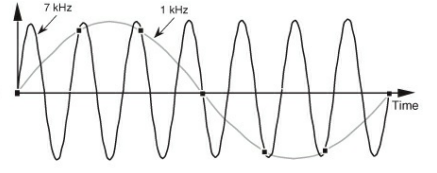
\includegraphics[width=0.75\linewidth]{Figures/aliasing.png}
                \caption[Aliasing example]{Example of aliasing, sampling analoge frequencies of 7 kHz and 1 kHz. Source:\cite{understanding_dsp}, Chapter 2}
                \label{fig:aliasing}
            \end{figure}

        \begin{equation}
        \label{eq:aliasing_x_n}
            x(n) = \sin{(2\pi f_0 n t_s)} = \sin{(2\pi(f_0 + kf_s) n t_s)} 
        \end{equation}
\newpage
        \subsubsection{The Half-Nyquist}
            The Half-Nyquist, is the frequency interval of Equation~\ref{eq:half_nyquist}, where after sampling the frequencies outside of this interval are aliased into this frequency band. This is useful, because it defines the unique frequency range that can be represented by the sampled signal, without ambiguity (\cite{understanding_dsp}, Chapter 2). 

    \begin{equation}
        \label{eq:half_nyquist}
        -\frac{fs}{2} < f <\frac{fs}{2}
    \end{equation}

    
    \begin{figure}[h]
        \centering
        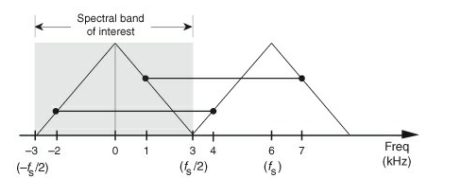
\includegraphics[width=0.75\linewidth]{Figures/half_nyquist.png}
        \caption[Nyquist example]{Example of Half Nyquist. Source:\cite{understanding_dsp}, Chapter 2.}
        \label{fig:half_nyquist}
    \end{figure}
   
    \subsection{Pulse Density Modulation (PDM)}
        \label{sec:PDM}

    % What is it? ok 
    % How does it represent the sound? Bit density? ok 
    % Use that as the reference:
    % - https://www.st.com/resource/en/application_note/an5027-interfacing-pdm-digital-microphones-using-stm32-mcus-and-mpus-stmicroelectronics.pdf
    % -https://users.ece.utexas.edu/~bevans/courses/rtdsp/lectures/10_Data_Conversion/AP_Understanding_PDM_Digital_Audio.pdf

    % REMEMBER TO MENTION THAT PDM IS EQUIVALENT TO THE SIGNAL FROM SIGMA_DELTA ADC !
    Pulse Density Modulation (PDM) is a method for representing the analoge sound signal as a high frequency bitstream of binary one and zero. The amplitude of the analoge signal is represented by increasing or decreasing the period of when the bianry '1' and '0' are present. If the density of '1' is high, the amplitude of the signal is positive, while the high density of '0' corresponds to the negative amplitude of the signal. Increase in the number of binary numbers may also correspond to the rate of change of the ampitude, signaling the rising or falling of the amplitude over time as shown in Fogure~\ref{fig:pdmvssinewave} (\cite{st_an5027_2019}, p.12). 

    \newpage
    \begin{figure}[h]
        \centering
        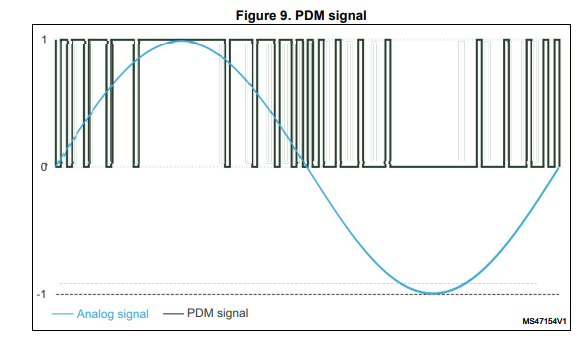
\includegraphics[width=0.75\linewidth]{Figures/PDM vs Sinewave from AN5027.png}
        \caption[Analoge and PDM signals]{Represntation of the analoge signal and it's corresponding PDM signal. Source:(\cite{st_an5027_2019}, p.12)}
        \label{fig:pdmvssinewave}
    \end{figure}

 % What is needed to "understand" the signal in this form? ok
 % The need of filtering and decimation of the signal? ok
    
    The digital microphones sending the PDM signal are able to send up to 3.25 Mbit/s of data, according to manual (\cite{st_mp34dt06j_2021}, Table 2, p.3), which can be unnececary overwhealming, and some of the operations, such as signal processing requires the use of PCM values. Thus the PDM to PCM conversion has to be applied (\cite{kite2012pdm}).


    \subsection{Pulse Code Modulation (PCM)}
    \label{sec:PCM}
    % What is a PCM signal?

    % https://books.google.no/books?hl=no&lr=&id=8l_o6kI3760C&oi=fnd&pg=PR13&dq=pulse+density+modulation+and+pulse+code+modulation&ots=nqlhYDIJRi&sig=ygAAOwsanJ5PmlTM_uisdlnUuIc&redir_esc=y&safe=strict#v=onepage&q=pulse%20density%20modulation%20and%20pulse%20code%20modulation&f=false

    %https://research.ebsco.com/c/qhbpyc/search/details/6evwwwovxr?request-context=plink&db=nlebk
    % https://users.ece.utexas.edu/~bevans/courses/rtdsp/lectures/10_Data_Conversion/AP_Understanding_PDM_Digital_Audio.pdf

    Pulse Code Modulation (PCM) is a method of representing the audio signal digitally, similarly to the PDM, with the main difference of storing the signal with more then just one bit. The method has two main properties needed to properly store the measured signal. It is the sampling rate, which dictates how many discrete samples per second are taken from the audio signal ,effectively limiting the bandwidth of the signal. The next property is the bit depth, or the wordlength, which determines the number of bits which represent each sample of the signal (\cite{st_an5027_2019}, p.12). Additionally the last property is also used to determine the theoretical Signal-to-Noise-Ratio (SNR) of each sample, based on the following Equation~\ref{eq:SNRWordLength} taken from (\cite{kite2012pdm}, p.4). The further explenation of SNR, can be found in the following Section~\ref{Sec:SNR} and the PCM is visualized in the following Figure~\ref{fig:PCM}.  

    \begin{equation}
        SNR = 6.02*N + 1.75
        \label{eq:SNRWordLength}
    \end{equation}

    \begin{figure}[h]
        \centering
        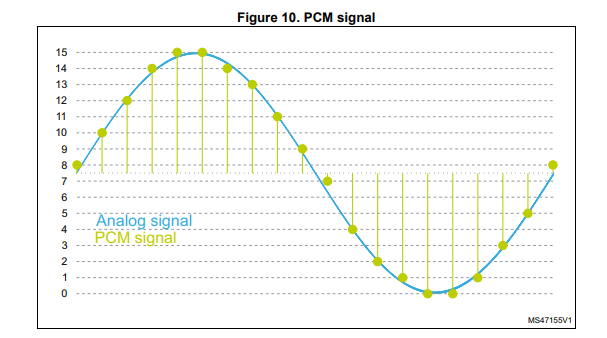
\includegraphics[width=0.75\linewidth]{PCM.png}
        \caption[Analoge and PCM signals]{Represntation of the analoge signal and it's corresponding PCM signal. Source:(\cite{st_an5027_2019}, p.13)}
        \label{fig:PCM}
    \end{figure}
    
\newpage
    
    \subsection{PDM to PCM Conversion}
    \label{sec:PDMtoPCM}

     To correctly convert the PDM into PCM signal, the sample rate of PDM has to be reduced, by a "decimation" factor, (where the dacimtation is the name of the reduction process) to achive the desired sampling frequency of the PCM signal. Decimation also works as the filtering procedure, where the samples outside of the passbond, are removed to reduce the influence of the noise onto the signal (\cite{kite2012pdm}, p.8 and \cite{st_an5027_2019}, p.13).

    
    % https://books.google.no/books?hl=no&lr=&id=8l_o6kI3760C&oi=fnd&pg=PR13&dq=pulse+density+modulation+and+pulse+code+modulation&ots=nqlhYDIJRi&sig=ygAAOwsanJ5PmlTM_uisdlnUuIc&redir_esc=y&safe=strict#v=onepage&q=pulse%20density%20modulation%20and%20pulse%20code%20modulation&f=false

    %https://research.ebsco.com/c/qhbpyc/search/details/6evwwwovxr?request-context=plink&db=nlebk
    % https://users.ece.utexas.edu/~bevans/courses/rtdsp/lectures/10_Data_Conversion/AP_Understanding_PDM_Digital_Audio.pdf
    
    % Low-pass filtering? ok
    % Decimation? ok
    % how does it reconstruct the amplitude?
    % Add nyquist (maybe)?

    

    \subsection{Signal-to-Noise-Ratio (SNR)}
    
    \label{Sec:SNR}

    It is assumed that most of the audio signals measured by the microphones contain a certain level of noise. To quantify the level of noise relative to the actual signal,
    the Signal-to-Noise-Ratio (SNR) is used.
    
    The SNR is defined as the ratio of power between the noise-free signal, and the total measured noise. The value is represented in dB, and can be either negative which represents the stronger noise power over the desired signal or the opposite with the positive value.
    SNR can be estimated using the following Formula~\ref{eq:SNR}, which was taken from (\cite{understanding_dsp}, Appendix D, Sections D5-D5.1).
    
    \begin{equation}
        \label{eq:SNR}
        SNR_{dB} = 10 \log_{10}(\dfrac{P_{signal}}{P_{noise}})
    \end{equation}

\section{Frequency-domain analysis}
This section presents the theoretical background for the frequency-domain analysis methods used in the project.

\subsection{Frequency Transform}
    The Frequnecy Transform (FT) is a method of representing a continous time domain signal, as a continous and infinite frequency domain signal, by using the following Equation~\ref{eq:FT} taken from (\cite{understanding_dsp}, p.74). The frequency domain representation provides the inforamtion of which frequency components are present in the signal, and how strong they are,

    \begin{equation}
    \label{eq:FT}
    X(f) = \int_{-\infty}^{+\infty} x(t) e^{-j 2\pi f t} \, dt
    \end{equation}

    \subsubsection{Discrete Fourier Transform}
    \label{sec:FFT}
    % explain general framing
    % explain general windowing 
    % explain spectral leakage
    Discrete Fourier Transform (DFT) represent a finite discrete-time signal as a discrete signal in the frequency domain. It is a variation of the Fourier Transform (FT) that can be easly understood by the modern machines due to the discrete nature of the output signal, that holds the spectral information such as the signal amplitude and the signal's phase. To apply the DFT, it has to be provided the discrete input signal, which has to be discretized, if originally being obtaing in the analoge form. The DFT represented by the following Equation~\ref{eq:DFT}, taken from (\cite{understanding_dsp}, p.75), uses the provided samples, to convert the signal into equally spaced frequency points which holds the previously mentioned spectral inormation. The frequncy points depend on frequency sampling (fs) and the number of samples (N). An increase of both of the values, may result in more detailed output signal, as the higher number of (N) provides the DFT with finer resolution, and the higher (fs) provides a larger frequency range (\cite{understanding_dsp}, p.74-76). On the other hand the increase of (N) may result in higher compuatational demand, due to the direct dependence of the transform on ($N^2$) as proved by Equation~\ref{eq:O_DFT}, inspired by (\cite{oppenheim_dft_lecture}, p.6) and (\cite{moler_eddins_fft}).

    \begin{equation}
    \label{eq:DFT}
    % taken from understanding..... 3-2 p74/75
        X(m) = \sum_{n=0}^{N-1} x(n) e^{-j 2\pi mn / N}
    \end{equation}

    \begin{equation}
        \label{eq:O_DFT}
        DFT_{computational \ complexity } = O(N^2)
    \end{equation}
    \subsubsection{Fast Fourier Transfor}
    \label{sec:FFT}
    To solve the problem, of DFT puting a high computational demand on the computer systems, the Fast Fourier Transform (FFT) was developed by John Cooley and John Tukey in 1965 (\cite{understanding_dsp}, p.138).
    The FFT and specifically radix-2 FFT is "a very effieicent alogrithm" (\cite{understanding_dsp}, p.138) that simplifies the DFT by eliminating the need of computing the redundant values, by "exploiting symmetry and periodicity properties of the complex exponential sequences" (\cite{oppenheim_dft_lecture}.p6).
    Hence the algorithm allows to conduct DFT of many samples in much reduced time, as the need for computation is greatly reduced as proved in Equation~\ref{eq:O_FFT}, taken from (\cite{understanding_dsp}, p.139). The superiority of FFT over DFT in terms of the reduced number of computations can be visualized by the Figure~\ref{fig:DFTvsFFT}]. However according to \cite{goyal2015condition}, p.8, the FFT has restricitions which doesn't allow it to depict spectral changes of the signal over time, which forces the implemnetation of Short-time Fourier Transform (STFT) which is used to extract the content of the non-stationary signal, such as sound produced by a moving drone. The STFT is conducted by framing the signal into short windows as that assumes stationary of the signal and then by applying the FFT on each window (\cite{goyal2015condition}, p.8).     

    \begin{figure}[h]
        \centering
        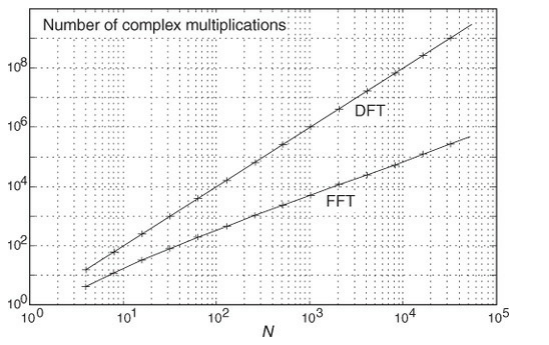
\includegraphics[width=0.5\linewidth]{DFTvsFFT.png}
        \caption[Number of complex multipliactions]{Number of complex mulitplications as a function of N, for FFT and DFT, Source:(\cite{understanding_dsp}, p.139)}
        \label{fig:DFTvsFFT}
    \end{figure}

    \begin{equation}
    \label{eq:O_FFT}
        FFT_{computational \ complexity} =O(\frac{N}{2}\log_2N)
    \end{equation}
\newpage
    \subsubsection{IDFT}
    \label{sec:IFFT}

    Inverse Discrete Fourier Transfrm (IDFT) is a method of converting the frequency domain signal into the time domain. The method may be applied, when the signal has been filtered, or modified in the frequency domain, but it's final form has to be represented in the time domain. The method is applied by utilizing the Equation~\ref{eq:IDFT}, taken from (\cite{understanding_dsp}, p.92) 

    \begin{equation}
    \label{eq:IDFT}
    x(n) = \frac{1}{N} \sum_{m=0}^{N-1} X(m) e^{j 2\pi m n / N}
\end{equation}

    \subsection{Windowing}
    \label{sec:Windowing}
    Windowing is a way of reducing the results of the spectral leakge, which occurs when there exists frequency components inside of the measured signal, that are not exactly represented by the fundamental frequency Equation~\ref{eq:f_fund}), and by it's integer multiplies (commonly known as the analysis frequencies). The analysis frequency can be found by utilizing Equation~\ref{eq:f_analysis} taken from (\cite{understanding_dsp}, p.92). The result of the spectral leakge may be described as a leakge of energy, that spreads into multiple frequency bins, outputted by the DFT and is visualized in the Figure~\ref{fig:Leakages}. The spectral leakge, is a persistent issue, that effects can only be minimized and not fully adressed (\cite{understanding_dsp}, p.92-95). One of the methods used to minimize the issue, is the application of windowing functions, such as Hanning or Hamming functions, that froces the amplitude of the finite signal at the begining and at the end of the signal segment to move towards zero, as seen in Figure~\ref{fig:windows}. As the DFT can only be applied on the finite time signals, the signal is by default windowed using the rectangle function, which causes the amplitude of the signal to sharply move from 0 to 1. That sharp move is the reason for the existance of the sidelobes in DFT magnnitude output, which also causes the spectral leakage as visualized in Figure~\ref{fig:sidelobes_windowing_effects}. The figure also proves that Hanning and Hamming would be the most suitable for the project application, due to their reduction of the sidelobes, which also reduces the leakage of energy into neighboring bins (\cite{understanding_dsp}, p.99-102).

\begin{equation}
\label{eq:f_fund}
    f_{fundamental} = \frac{fs}{N}
\end{equation}

\begin{equation}
\label{eq:f_analysis}
    f_{\text{analysis}}(m) = \frac{m f_s}{N}, \quad \text{where } m = 0,1,2,\ldots,N-1
\end{equation}
    
\begin{figure}[H]
    \centering
    
    \begin{subfigure}{0.45\linewidth}
        \centering
        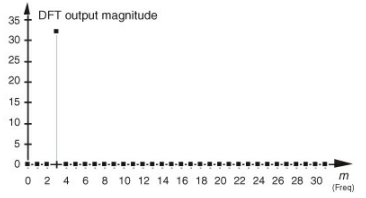
\includegraphics[width=\linewidth]{Figures/No_leakage.png}
        \caption{Magnitude of the DFT without the leakge}
    \end{subfigure}
    \hfill
    \begin{subfigure}{0.45\linewidth}
        \centering
    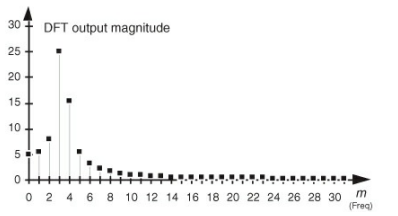
\includegraphics[width=\linewidth]{Figures/leakage_present.png}
        \caption{Magnitude of the DFT with leakge present}
    \end{subfigure}
\caption[Response without the leakage vs with the leakage]{Comparison between the DFT magnitude without the leakage and with the leakge present. Source: \cite{understanding_dsp}, p.93-94}
    \label{fig:Leakages}
\end{figure}


\begin{figure}[H]
    \centering
    
    \begin{subfigure}{0.45\linewidth}
        \centering
        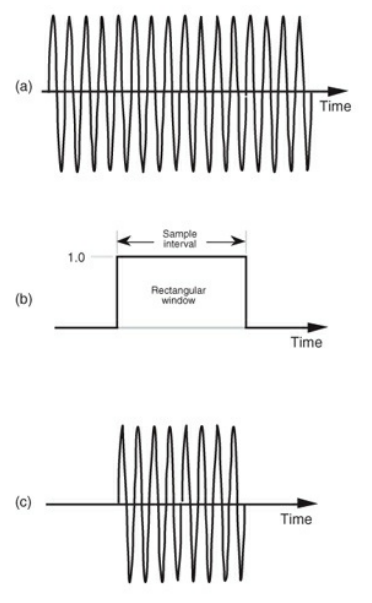
\includegraphics[width=\linewidth]{rectangle.png}
        \caption{Rectangular window}
    \end{subfigure}
    \hfill
    \begin{subfigure}{0.45\linewidth}
        \centering
        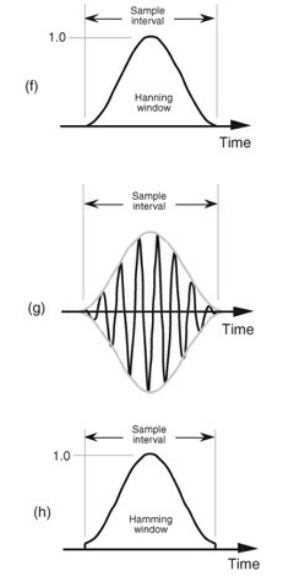
\includegraphics[width=\linewidth]{Hanning.png}
        \caption{Hanning window}
    \end{subfigure}
    
    \caption[Rectangular vs hanning window]{Comparison of rectangular and Hanning window functions and the result of applying them on the infinite time signal. Source: \cite{understanding_dsp}, p.100}
    \label{fig:windows}
\end{figure}

\begin{figure} [H]
    \centering
    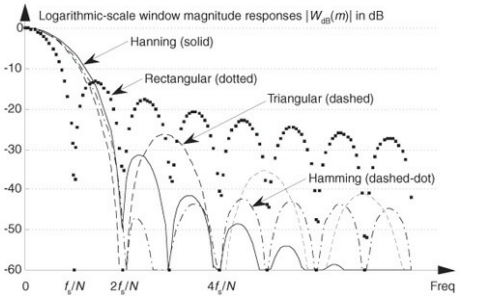
\includegraphics[width=0.75\linewidth]{Figures/sidelobes_windowing.png}
    \caption[Windowing effects]{Effects of windowing functions on side lobe creation. Source: \cite{understanding_dsp}, p.102}
    \label{fig:sidelobes_windowing_effects}
\end{figure}

\subsection{Sinc function as a digital filter}
\label{sec:sinc_filter}
The sinc function can be expressed as in the following Equation~\ref{eq:sinc}, taken from \cite{understanding_dsp}, Section 3.8, though a bit modified to represent the continous function. The function represents the behaviour of the moving-average filter, where the input data is averaged over the set number of previous samples (\cite{stm_an4990_dfsdm}, Section 3) as in the following Equation~\ref{eq:moving_average} from (\cite{understanding_dsp}, Section 10.14.1). The filter can be designed as described in Figure~\ref{fig:moving_avg_schematic}, however the D, has be changed with FOSR in the schematic, but they still represent the same number. Additionaly the digtal signal that has been filtered, can be processed again, if the higher order of the sinc function is applied. However the additional processing of the signal, in addition to attenuating the unwanted frequencies, can also attenuate the desired frequencies as in the concept figures: Figure~\ref{fig:comparison_of_signals_with_sinc} and Figure~\ref{fig:mag_response_sinc}, where the aplication of the 3rd-order sinc reduces the original signals magnitude to around 37\% of the original value, despite the reduction of the side lobes.


\begin{equation}
    \label{eq:sinc}
    sinc(x) = \frac{\sin(\pi x)}{\pi x}
\end{equation}

\begin{equation}
    \label{eq:moving_average}
    y(n) = \frac{1}{D}[x(n) + x(n-1) + ... + x(n - D + 1)] = \frac{1}{D}\sum^{D-1}_{k = 0}x(n-k)
\end{equation}

\begin{figure}[h]
    \centering
    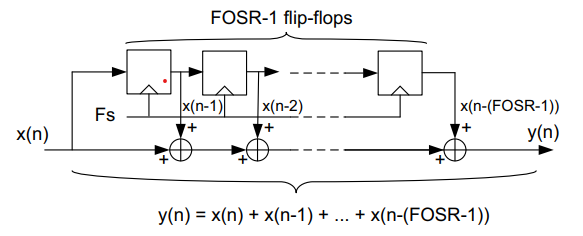
\includegraphics[width=1\linewidth]{Figures/basic_moving_avg_schematic.png}
    \caption[Moving average example]{A basic schematic for a moving average filter. Source: \cite{stm_an4990_dfsdm}, Figure.10}
    \label{fig:moving_avg_schematic}
\end{figure}

\newpage

\begin{figure}[h]
    \centering
    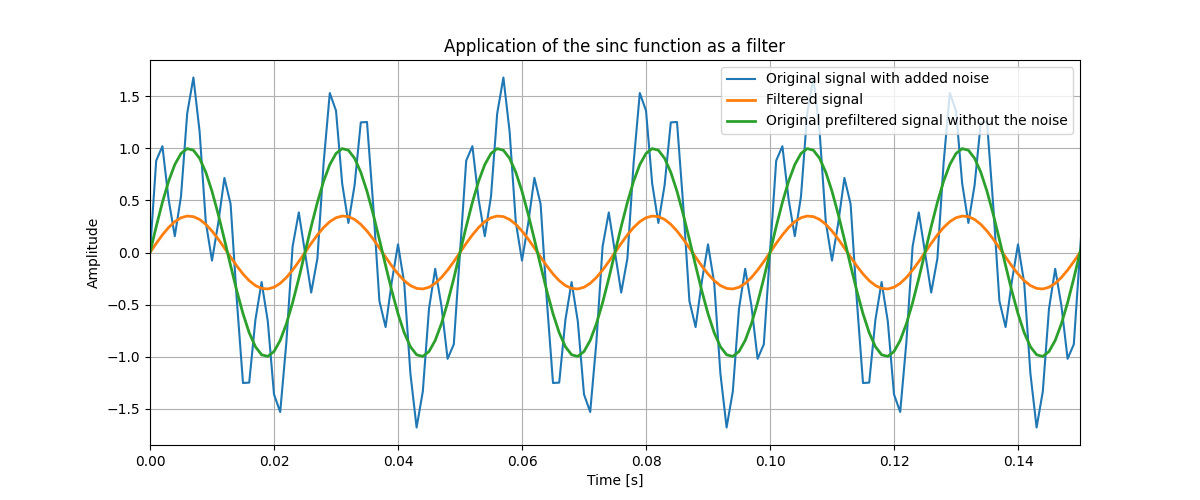
\includegraphics[width=1\linewidth]{filtering of a signal with sinc.png}
    \caption[Original vs filtered signal example]{Comparison of the original signal ($\sin{(2\pi 40t)})$, with added noise of $0.7\sin{(2\pi 180t)}$, and the final signal filtered with the sinc function and the sampling frequency of 1000. }
    \label{fig:comparison_of_signals_with_sinc}
\end{figure}

%wanted = np.sin(2 * np.pi * f_wanted * t)
%unwanted = 0.7 * np.sin(2 * np.pi * f_unwanted * t)

\begin{figure} [h]
    \centering
    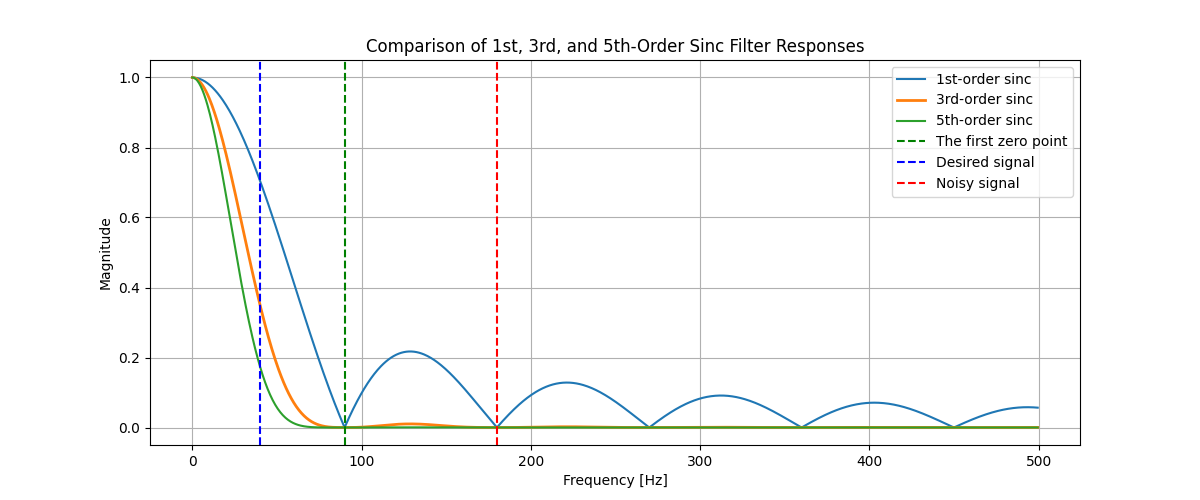
\includegraphics[width=1\linewidth]{Figures/sinc function mag responses.png}
    \caption[Example responses of the sinc based filters]{Magnitude responses of sinc based filters of different order}
    \label{fig:mag_response_sinc}
\end{figure}


\newpage

\section{Direction of arrival (DOA) estimation}
   The Direction of arrival (DOA) describes the direction from which the acoustic signal reaches the microphones. The DOA can be estimated by measuring the Time difference of arrival (TDOA) between microphone pairs and relating theses delays to the physical geometry of the microphone array, and the sound speed as expressed in Equation~\ref{eq:tau}. In this relation, \textbf{d} represents the distance between the microphone in the pair, \textbf{c} stands for the sound speed and \textbf{$\theta$} denotes the angle of arrival of the sound source relative to the normal vector of the microphone pair (\cite{blandin2012multisource}). The relation is valid under the far-field assumption, which assumes that the distance between the sound source and the microphone array is larger then the distance between the microphones.   

    \begin{equation}
        \label{eq:tau}
        \tau = \frac{d}{c}\cos(\theta)
    \end{equation}

    \subsection{Time Difference of Arrival (TDOA)}
    \label{sec:TDOA}
    % Propagation delay
    % Geometry
    % Relationship between the distance and delay and angle 
    % Limitation caused by tge mic spacing
    % Max phisically possible lag
    % Near filed and far filed assumptions
    The Time Difference of Arrival (TDOA) represents the time difference in arrival time of the acoustic signal between a pair of spatially separated microphones. Effectively representing which microphone in the pair, was first to receive the acoustic signal. To achieve that, the project uses the generalized cross-correlation (GCC) which estimates the TDOA of a microphone pair, and later uses the microphone geometry to estimate the direction of arrival (DOA) of the signal source (\cite{kwon2010gccphat}, \cite{blandin2012multisource} and \cite{kang2016prefiltering}). 


    \subsection{Generalized Cross-Correlation with PHAT weighting (GCC-PHAT)}
    \label{sec:gcc}
    The GCC represents the degree of correlation between the signals from a microphone pair over different time lags. The correlation is computed in frequency domain by finding the cross-power spectrum (CPS) of the microphone pair. In GCC-PHAT, the CPS is adjusted by PHAT weighting with additional factor $\beta$, which reduces the influence of large-amplitude frequency components and makes the TDOA estimation more dependent on the phase difference between the microphone signals. %This may improve the robustness of the delay estimation, although noisy frequency components can still affect the result 
    (\cite{kang2016prefiltering} and \cite{kwon2010gccphat}).
    
    \subsubsection{Cross-power spectrum (cps)}
    \label{sec:cps}
    The Cross-power spectrum between the microphones, is found by multiplying the frequency-domain signal from one microphone, with the conjugate of the signal from the second microphone as in the following Equation~\ref{eq:gcc}. % from \cite{kang2016prefiltering}.
    The output of the CPS represents the relation between the microphone signals for each frequency bin $k$, which includes the magnitude relationship and the phase difference caused by the time delay between the microphones (\cite{kang2016prefiltering}).

    \begin{equation}
    \label{eq:gcc}
        G(k) = X_1(k)X_2^*(k)
    \end{equation}


    \subsubsection{PHAT weighting}
    \label{sec:PHatW}
    PHAT weighting 
    is used to reduce the influence of the high amplitude frequencies, that may shadow other, weaker frequency components, by normalizing the amplitudes of their CPS values as in the Equation~\ref{eq:phat}. Additionally the PHAT can be adjusted by the $\beta$ weight, that may vary from 0 to 1, based on the SNR value, or any other application-specific criteria (\cite{kang2016prefiltering}).       

    \begin{equation}
        \label{eq:phat}
        \Psi^\beta (k) = \frac{1}{|G(k)|^\beta}
    \end{equation}
    
    \subsubsection{Delay estimation from the GCC function}
    \label{sec:delay_estimation_from_gcc}
        The time differnce can be estimated by finding the lag that is maximizing the GCC-PHAT output as in the following Equation~\ref{eq:r_l} %from \cite{kang2016prefiltering}
        , where the GCC output is weighted by the PHAT function and then transformed back to the time-domain (\cite{kang2016prefiltering}).

    \begin{equation}
        \label{eq:r_l}
        \max r(l) = F^{-1}(\Psi^{\beta}(k)G(k))
    \end{equation}

    
\section{Feature extraction}
This section presents the theoretical background for the feature extraction methods used in this project.

    \subsection{Mel scale}
    \label{sec:MEL}

    The Mel scale is a frequency scale that approximates how humans perceive pitch. In MFCC feature extraction, the power spectrum \(P(f)\) is wraped from the Hertz frequency axis to the Mel-frequency axis as \(P(M)\) in order to approximately reflect human ear percetion. A frequency \textbf{f} in Hertz can be converted to the mel scale as in the Equation~\ref{eq:mel} (\cite{zheng2001mfcc}).


    \begin{equation}
        \label{eq:mel}
        M(f) = 2595\log_{10}(1+\frac{f}{700})
    \end{equation}

    \subsection{Mel-frequency cepstral coefficients (MFCC) }
    \label{sec:MFCC}
    The MFCC is a feature extraction method used to represent the short-term spectral characteristics of an acoustic signal. The information about spectral characteristics is stored in the MFC coefficients, which number can vary, and can either increase or decrease the computational time needed to extract the features. To extract the MFCC features, the extraction algorithm can follow the following pipeline Figure~\ref{fig:mfcc_pipeline} (\cite{singh2014mfcc}).

    \begin{figure}[h]
        \centering
        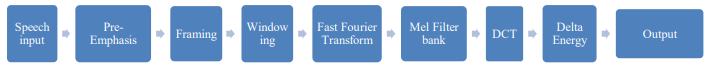
\includegraphics[width=1\linewidth]{Figures/MFCC_pipeline.png}
        \caption[Example pipeline for MFCC]{Example pipeline for the extraction of the MFCC features. Source: \cite{singh2014mfcc}}
        \label{fig:mfcc_pipeline}
    \end{figure}

    \subsubsection{Pre-emphasis}
    \label{sec:pre_emp}
    The pre-emphesis stage of the MFCC extraction is used to emphasize the higher-frequency components present in the signal before the further feature extraction. This increases the energy levels of the high-frequency components present in the measured signal (\cite{singh2014mfcc} and \cite{librosaPreemphasis}). An example of how the pre-emphesis can change the signals energy content can be seen in Figure~\ref{fig:pre-emphesis example}.

    \begin{figure}[h]
        \centering
        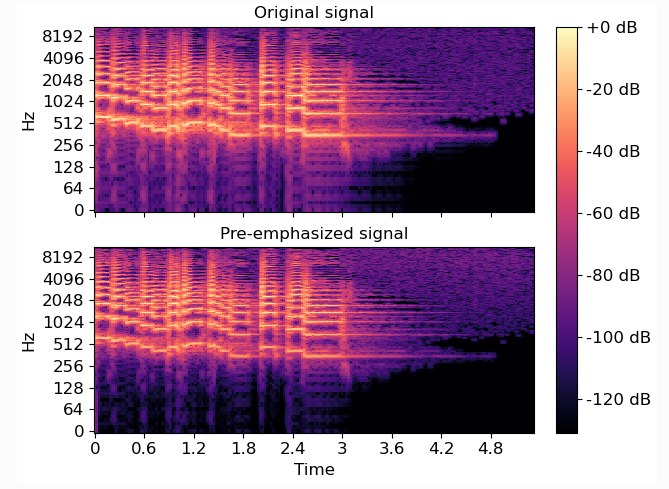
\includegraphics[width=0.5\linewidth]{Figures/example of pre-emphesis.png}
        \caption[Pre-emphesis example]{An example of how the pre-emphesis can change the energy content of the signal. Source:\cite{librosaPreemphasis}}
        \label{fig:pre-emphesis example}
    \end{figure}
    
    \subsubsection{Framing}
    Framing is used to divide the signal into short-duration frames because of the time-varying nature of acoustic signals. Within a short frame such as 25 ms, the signal can be treated as approximately stationary, since the frame contains data from only a short time interval (\cite{singh2014mfcc}).

    
    \subsubsection{Mel filter bank (MLB)}
    The MLB is used to convert the signal's magnitude response in the frequency domain to the mel-scale based response. This is achived by multiplying the magnitude response of the signal with a set of K-number band-pass filters of triangular or rectangular shape wich may, or may not overlap with each other. The filter forms can be as in the Figure~\ref{fig:band_pass_filters} (\cite{singh2014mfcc} and \cite{zheng2001mfcc}).


    \begin{figure} [h]
        \centering
        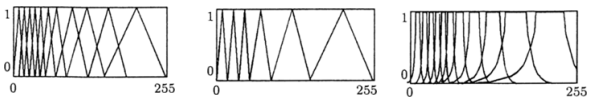
\includegraphics[width=1\linewidth]{Figures/mel_bank_filters.png}
        \caption[Band-pass filter]{The Band-pass filters used in the process of extraction the MFCC. Source: \cite{zheng2001mfcc}}
        \label{fig:band_pass_filters}
    \end{figure}

    % Should i even write about that, if I have no use to that in the method? However i do use the default type 2 DCT, when using MFCC from librosa 
    %\subsubsection{Discrete Cosine Transform (DCT)}
    %The DCT 

    \subsection{Delta and Delta-Delta features}
    \label{sec:deltadelta}
    The delta and delta-delta represents the rate of change, and acceleration of the cepstrum represented by the MFCC. The delta can be found by taking the first-order time derivative and the delta-delta by the second-order time derivative (\cite{singh2014mfcc}).
    

\section{ML classification}
\subsection{YOLO Object Detection}

YOLO (You Only Look Once) is a real-time single-stage object detection 
model based on Convolutional Neural Networks (CNNs). Unlike two-stage 
detectors such as Faster R-CNN, which require separate region proposal 
and classification passes, YOLO divides the input image into a grid and 
performs both object localization and classification in a single forward 
pass, achieving significantly faster inference speeds (\cite{redmon2016yolo}). 
Where R-CNN takes around 47 seconds to process a single image due to 
classifying approximately 2000 region proposals, YOLO processes the entire 
image in one shot, making it far more suitable for time-sensitive 
applications (\cite{vijayakumar2024yolo}). Since its introduction in 2015, 
the model has undergone continuous architectural refinement, with each 
version addressing specific limitations of its predecessor 
(\cite{vijayakumar2024yolo, sapkota2025ultralytics}).

\vspace{1em}

Key milestones in this evolution include YOLOv2, which introduced anchor 
boxes and batch normalization (\cite{vijayakumar2024yolo}); YOLOv3, which 
deepened the backbone to Darknet-53 and added multi-scale feature 
prediction through a Feature Pyramid Network (FPN) (\cite{vijayakumar2024yolo}); 
and YOLOv4, which incorporated CSPDarknet-53, a Path Aggregation Network 
(PANet) neck, and the CIoU loss function (\cite{vijayakumar2024yolo}). 
YOLOv5 marked a decisive shift to a fully PyTorch-native implementation, 
introducing five modular depth- and width-scaled variants and a unified 
training and export toolchain (\cite{vijayakumar2024yolo, sapkota2025ultralytics}).


\subsection{YOLOv8 Architecture}

YOLOv8, released by Ultralytics in January 2023, follows the standard 
three-part structure of backbone, neck, and head that became established 
from YOLOv3 onwards (\cite{vijayakumar2024yolo}), and introduces targeted 
improvements at each stage (\cite{vijayakumar2024yolo, sapkota2025ultralytics}).

\vspace{1em}

The \textbf{backbone} replaces earlier C3 modules with a new C2f module 
--- a Cross Stage Partial structure incorporating two convolutional 
operations and a bottleneck --- which maintains receptive-field richness 
while reducing parameter overhead (\cite{sapkota2025ultralytics}). A Spatial 
Pyramid Pooling Fast (SPPF) layer follows the backbone to aggregate 
context across multiple spatial scales (\cite{sapkota2025ultralytics}). The 
\textbf{neck} uses a PANet-style structure to combine top-down and 
bottom-up pathways, ensuring that both high-level semantic information and 
fine-grained spatial detail flow into the head (\cite{vijayakumar2024yolo}).

\vspace{1em}

The most significant change in YOLOv8 is the fully \textbf{decoupled 
detection head}, which separates the classification and bounding box 
regression branches into two independent streams (\cite{sapkota2025ultralytics}). 
This mitigates gradient interference between the two objectives and 
improves convergence (\cite{sapkota2025ultralytics}). Complementing this, 
YOLOv8 adopts a fully \textbf{anchor-free} design, directly predicting 
normalized bounding box parameters for candidate points on the feature 
map, removing the need for anchor clustering and improving generalization 
across datasets with differing object aspect-ratio statistics 
(\cite{vijayakumar2024yolo, sapkota2025ultralytics}). For bounding box 
regression, YOLOv8 uses the CIoU loss function, and binary cross-entropy 
for classification (\cite{vijayakumar2024yolo}). Following inference, 
Non-Maximum Suppression (NMS) is applied to suppress redundant overlapping 
detections, retaining only the highest-confidence bounding box for each 
object (\cite{vijayakumar2024yolo}).

\vspace{1em}

YOLOv8 is offered in five scaled variants --- nano (n), small (s), 
medium (m), large (l), and extra-large (x) --- which differ in network 
depth and width (\cite{sapkota2025ultralytics}). This thesis uses 
\textbf{YOLOv8n}, the nano variant, which has approximately 3.2 million 
parameters and 8.7 billion FLOPs (\cite{sapkota2025ultralytics}). On the 
MS COCO validation set at 640$\times$640 pixel input resolution, YOLOv8n 
achieves a mean Average Precision (mAP@0.50:0.95) of approximately 37.3\%, 
with a CPU latency of around 80.4\,ms per image (ONNX) and under 1\,ms 
on an NVIDIA T4 GPU (TensorRT) (\cite{sapkota2025ultralytics}).


\subsection{Performance Metrics}

Object detection performance is primarily evaluated using \textbf{Intersection 
over Union (IoU)} and \textbf{mean Average Precision (mAP)} 
(\cite{vijayakumar2024yolo}). IoU measures the spatial overlap between a 
predicted bounding box and the ground-truth box, calculated as the ratio 
of their intersection to their union area, ranging from 0 to 1 
(\cite{vijayakumar2024yolo}). A detection is considered correct only when 
its IoU with the matched ground truth exceeds a set threshold, most 
commonly 0.5 (\cite{vijayakumar2024yolo, sapkota2025ultralytics}).

\vspace{1em}

Precision measures the proportion of predicted detections that are 
correct (TP / (TP + FP)), while Recall measures the proportion of actual 
objects that are successfully detected (TP / (TP + FN)) 
(\cite{vijayakumar2024yolo}). Average Precision (AP) is computed as the 
area under the precision--recall curve for a single class, and mAP 
averages this over all classes (\cite{vijayakumar2024yolo}). YOLO models 
use mAP as the primary metric in preference to the F1 score, as the 
F1 score can be heavily skewed toward majority classes in datasets with 
class imbalance, making it unreliable for evaluating performance on 
minority classes (\cite{vijayakumar2024yolo}). The stricter COCO-style 
evaluation reports mAP@0.50:0.95, averaging AP over ten IoU thresholds 
from 0.50 to 0.95 in steps of 0.05, penalizing imprecise localization 
more heavily than the older Pascal VOC standard (\cite{sapkota2025ultralytics}).

\subsection{Sound classification}
\subsubsection{Convolutional Neural Network}
A Convolutional Neural Network(CNN) is a deep-learning architecture inspired by human pattern recognition. CNNs consist of an input layer, one or more hidden layers, and an output layer, through which they learn to recognise patterns in visual data. The input layer performs pre-processing(e.g., rescaling, normalisation) to bring each image into a standardised representation for further computation. The Hidden part of the model may contain several layer types, including convolutional layers, pooling layers, and fully‑connected layers. Among these the convolutional layer is key: it applies a set of learnable filters to the input, extracting local features and producing a feature map for each filter. Finally the output layer combines the information from the hidden layers into class-probability estimates.(\cite[Chapter 14]{geron2019handson})
\subsubsection{Decision tree}
Decision‑tree learning is a supervised‑learning algorithm that maps a set of input variables onto a target variable. Two main variants exist: classification trees, which predict a categorical class label, and regression trees, which predict a continuous outcome. In the context of this paper, only the classification variant is relevant, whereby the model assigns each input value to one of the predefined classes.(\cite[Chapter 6]{geron2019handson})
        
\section{Hardware}
    This section provides a brief and general description of the hardware present in the system. 
        \subsection{Digital MEMS microphones}
        % WORK IN PROGRESS
        The digital mems microphones, as seen in the example schematic Figure~\ref{fig:mems_block}, are consturated in such a way, that they can convert the acoustic signal (which is in the analog form) into the digital PDM format,easily readable by the peripheral at the MCU.
        The data send from the microphones is controlled by the frequency of the \textbf{CLK} input, which typically is provided a High/Low signal at the frequency between 1 Mhz to 3 Mhz by the connected MCU. 
        The microphones can also allow to select at which moment the microphone should send the data, based on the connection to the \textbf{Channel select}, as in Figure~\ref{fig:stereo_mics}.

        \begin{figure}[h]
            \centering
            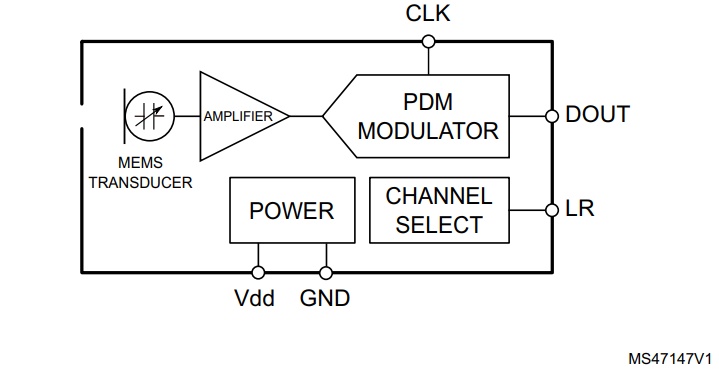
\includegraphics[width=0.75\linewidth]{Figures/mems_mics.png}
            \caption[Example block diagram of mems microphone]{Example block diagram of a mems digital microphone. Source: \cite{st_an5027_2019}}
            \label{fig:mems_block}
        \end{figure}

        \begin{figure}[h]
            \centering
            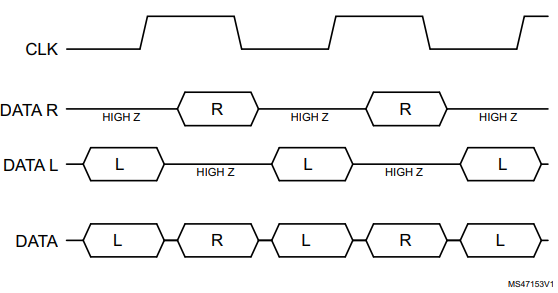
\includegraphics[width=0.75\linewidth]{Figures/stereo_mics_config_data.png}
            \caption[Stereo data pattern]{The Stereo data pattern from the mems microphones. Source: \cite{st_an5027_2019}}
            \label{fig:stereo_mics}
        \end{figure}
    
     % MEMS mics principle:
        % How do they work?
        % What do they need?
    % Analog vs digital mics
        % main differences, but reather short, as only teh digital mics were used.
     % Shared data line and time division
        % Clock signal?
        % Data line?
        % Selection of L/R on Mics?
        % Time multiplexing
    % Use that as the reference:
    % - https://www.st.com/resource/en/application_note/an5027-interfacing-pdm-digital-microphones-using-stm32-mcus-and-mpus-stmicroelectronics.pdf
    % - https://www.st.com/resource/en/data_brief/steval-mic002v1.pdf
    % -https://users.ece.utexas.edu/~bevans/courses/rtdsp/lectures/10_Data_Conversion/AP_Understanding_PDM_Digital_Audio.pdf 
        


        
\section{Communication protocols and peripherals}
    This section provides a theoretical description of the communication protocols present in the system.
    
    \subsection{Digital Filter Sigma-Delta Modulator (DFSDM)}
    The DFSDM is a digital peripheral used for processing and filtering of a 1-bit stream sent by the microphones. The example block diagram of the peripheral can be seen in Figure~\ref{fig:dfsdm_block}.
    The 1-bit stream is produced by a sigma-delta modulator (SDM), which converts the analog acoustic signal into a digital bitstream, as shown in Figure~\ref{fig:sdm}. In the project, the conversion is performed internally by the digital microphones, which outputs the signal as PDM.
    The converted signal is then sent to the microcontroller, where the Digital Filter (DF) applies the digital sinc function of configurable order, as described in Section~\ref{sec:sinc_filter}. The DF can be configured, by changing the order of the sinc function and the oversampling ratio known as FOSR. 
    The output data from the DF, can also be accumulated in the integrator, by changing the value of IOSR, which represents how many samples have to be summed up to return a single sample output. The final output data from the peripheral, is directly determined by the number of the PDM input samples, FOSR and the IOSR number. By changing any of them, the final sample rate will therefore vary. The peripheral to able to correclty process the data signal from the microphones, also has to generate the clock signal, that the microphone will adjust its data signal to (\cite{stm_an4990_dfsdm}).
    
    %The DFSDM uses the digital filter (DF) and the external Sigma-delta modulator (SDM), and as the name implies, filters the digital signal, by applying the sinc-function of freely chosen order, which was already described in more detail in this section [sec:\ref{sec:sinc_filter}. The SDM is responsible for converting the analoge signal into the digital signal that can be later filtered, as in the following schematic [fig:\ref{fig:sdm}]. The project is only using the SDM in such a way, that the microphones are internally converting the analoge acoustic signal into the PDM signal, most probably using the same principle, as described in the Sigma-delta modulation schematic. The converted signal is then sent to the microcontroller in the digital form to be filtered by the peripherial.    

    \begin{figure}[h]
        \centering
        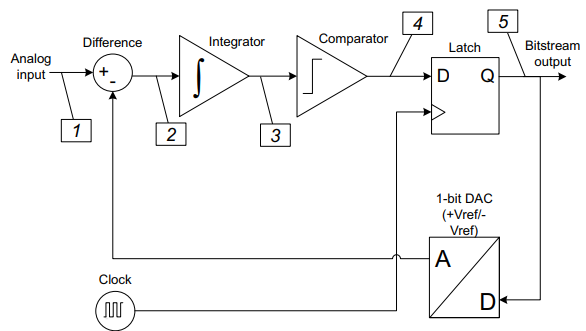
\includegraphics[width=0.5\linewidth]{Figures/sigma_delta_modulation.png}
        \caption[Example of a Sigma-delta modulator schematic]{Sigma-delta modulation schematic. Source: \cite{stm_an4990_dfsdm}}
        \label{fig:sdm}
    \end{figure}

    \begin{figure}[h]
        \centering
        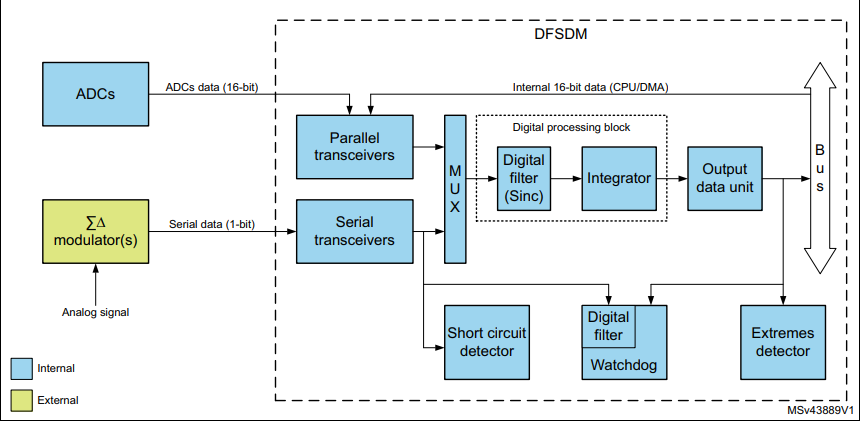
\includegraphics[width=0.5\linewidth]{Figures/dfsdm_internal_block.png}
        \caption[Example of a DFSDM block diagram]{DFSDM block diagram. Source: \cite{stm_an4990_dfsdm}}
        \label{fig:dfsdm_block}
    \end{figure}
    \newpage
    \subsection{Serial Audio Interface (SAI)}
    Tha SAI is an interface that can be used to receive the data signal from the digital microphones. The SAI can operate with its own audio clock generator, or the external timer, which can generate the clock signal for the microphones. The interface can operate with two sub-blocks, which can gather data independently. If the interface is gathering the data only from one microphone per line, the bit content should be as in the Figure~\ref{fig:mono_sai}, where the bits from the microphone are stored in a byte in the memory and accesd through the Direct Memory Acces (DMA). However When gathering the data from two microphones connected to the same line, the bit content will vary as it will be as in the Figure~\ref{fig:stereo_sai}, where each odd bit represent the data from one microphone, and the even one represent the second microphone. The resulting bit-stream from the microhpones is therefore interleaved, and need the additional de-interleaving algorithm to separate the bits from each other. (\cite{st_an5027_2019}).


\begin{figure}[h]
    \centering
    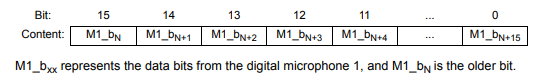
\includegraphics[width=0.75\linewidth]{mono_sai.png}
    \caption[Example of a mono bit configuration for SAI]{Bit configuration for the mono setup of SAI. Source: \cite{st_an5027_2019}}
    \label{fig:mono_sai}
\end{figure}



\begin{figure}[h]
    \centering
    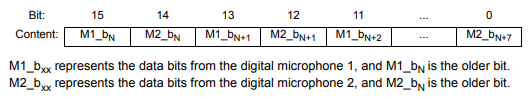
\includegraphics[width=0.75\linewidth]{Figures/stereo_sai.png}
    \caption[Example of a stereo bit configuration for SAI]{Bit configuration for the stereo setup of SAI. Source: \cite{st_an5027_2019}}
    \label{fig:stereo_sai}
\end{figure}
\newpage

    \subsection{USART/UART}
    Universal Synchronus/Asynchronus Receiver Transimter (USART/ UART) are variations of a communitation protocol used in the early stages of the project. The protocol is able to send the data from the transmitter in the asynchronus mode, where the receiver does not share the synchronization clock signal with the transmitter, hence it has to be manually configured before use with the same baud rate as the transmitter. However in the synchronus mode, the receiver and the transmitter both share the data and the clock lines, where the clock line aligns the data signal, without the need of prior data configuration. The frame format of a typical UART protocol is as in Figure~\ref{fig:uart_frame}, which contains the idle High bit, the low start bit , the data bit, the low parity bit and the high stop bit, which add up to 10 bits per second. Based on the following online calculator \cite{lucidar_baud_bytes}, the Bytes per second can be found by using the following Equation~\ref{eq:bytes_per_second_baud}
    where the \textbf{$BR_{bauds}$} represents the baud rate and the \textbf{bits per frame} are in this case equal to 10 bits per second per frame (\cite{stm_uart}, \cite{techtarget_usart} and \cite{laddha2013uart}).


    \begin{figure}[h]
        \centering
        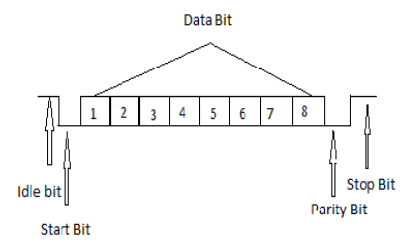
\includegraphics[width=0.5\linewidth]{Figures/uart_bit_map.png}
        \caption[Example of a UART frame format]{The typical UART frame format. Source: \cite{laddha2013uart}}
        \label{fig:uart_frame}
    \end{figure}

    \begin{equation}
        \label{eq:bytes_per_second_baud}
        BR_{gross} = \frac{BR_{bauds}}{bits \space  per \space frame}
    \end{equation}
    
    \subsection{USB}
    The Universal serial bus (USB) is a serial communication standard introduced to standardize the communication between the host and the device, and at the same time provide them with high speed transfer capabilities. The USB devices can be implemented using different device classes, which dictates how the devices will communicate with each other, depending on the devices application and function. The transfer speeds used by the USB 2.0, which was also used in the later stage of the project, can be divided into the following three categories:\\
    \\
    - Low speed (LS) which supports the speed of up to 1.5 Mb/s,\\
    - Full speed (FS) that can transfer the data with the speed of up to 12 Mb/s,\\
    - High speed (HS) which is the fastet one, providing the user with the transfer speed of up to 480 Mb/s.\\
    (\cite{stm_usb}).
    
    
    
    \subsection{MQTT}
    
Message Queue Telemetry Transport (MQTT) is a lightweight publisher/subscriber communication protocol designed for efficient message exchange. In a pub/sub system, publishers send messages to a named topic, which are then received by any clients subscribed to that topic. MQTT brokers act as intermediaries, holding and distributing messages between clients, which can function as both publishers and subscribers simultaneously (\cite{soni2017mqtt}).


    \subsection{UDP}
    
The User Datagram Protocol (UDP) is a connectionless transport protocol that sends
data packets without establishing a dedicated connection or guaranteeing delivery,
ordering, or error correction (\cite{rfc3550}). Unlike TCP, UDP does not retransmit
lost packets, which makes it particularly well suited for real-time video streaming.
In a live video feed, a retransmitted packet arriving late is more disruptive than
a dropped frame, as it introduces latency and stuttering that degrades the viewing
experience (\cite{rfc3550}). For this reason, real-time video applications commonly
rely on UDP as the underlying transport protocol, accepting occasional packet loss
in favour of low and consistent latency.

\subsection{H.264}

H.264, also known as MPEG-4 AVC, is a widely used video compression standard
developed jointly by the ISO/IEC MPEG group and the ITU-T Video Coding Experts
Group. Compared to its predecessor MPEG-2, H.264 achieves perceptually equivalent
video quality at roughly one-third to one-half of the bitrate, making it well suited
for bandwidth-constrained applications such as network video streaming (\cite{1709847}).

H.264 is a block-based hybrid video codec, meaning it reduces redundancy in video
data through a combination of motion compensation and transform coding. Video frames
are divided into $16 \times 16$ pixel macroblocks, which are processed using one of
several frame types: intra-coded (I), predictive (P), or bipredictive (B) frames
(\cite{1709847}).

\subsection{Project Management}
Scrum is an agile project‑management framework designed to coordinate complex, knowledge‑intensive initiatives through iterative and incremental development. Scrum Organizes its workflow into sprints. Sprints are short time periods usually chosen to be one to four weeks. At the end of the sprint a meeting is held to walk through the achieved goals and the goals for the next sprint. There usually also is frequent meetings during the sprint to check up on progress. Scum is based on three different roles:the Product Owner, Scrum Master, and Developers. The Product Owner manages priorities and stakeholder requirements, the Scrum Master manages and controls the Scrum process, and Developers are responsible for developing products according to the timeline.\cite{SchwaberSutherland2020}
\clearpage


\chapter{Methods}
% Hvordan implementerte jeg dette i praksis?


% Data aquisition 
% DATA transfer
% Offline processing
% feature extraction

%\section{System Architecture}
%    \subsection{Block Diagram} 
%    \subsection{Signal Flow}

\section{3D design}
\subsection{PAN and Tilt mechanism}

The camera platform is a modified version of this pan tilt camera setup (\cite{isaac879_2020_pantilt}) with all files being created using fusion 360. At first a Prusa Slicer mini with 0.4mm nozzle diameter was used for the intial prints. With the later prints being done using a Bambu lab P2S  3D printer with a 0.4mm nozzle diameter. 

\begin{figure}[H]
    \centering
    \begin{subfigure}{0.45\linewidth}
        \centering
        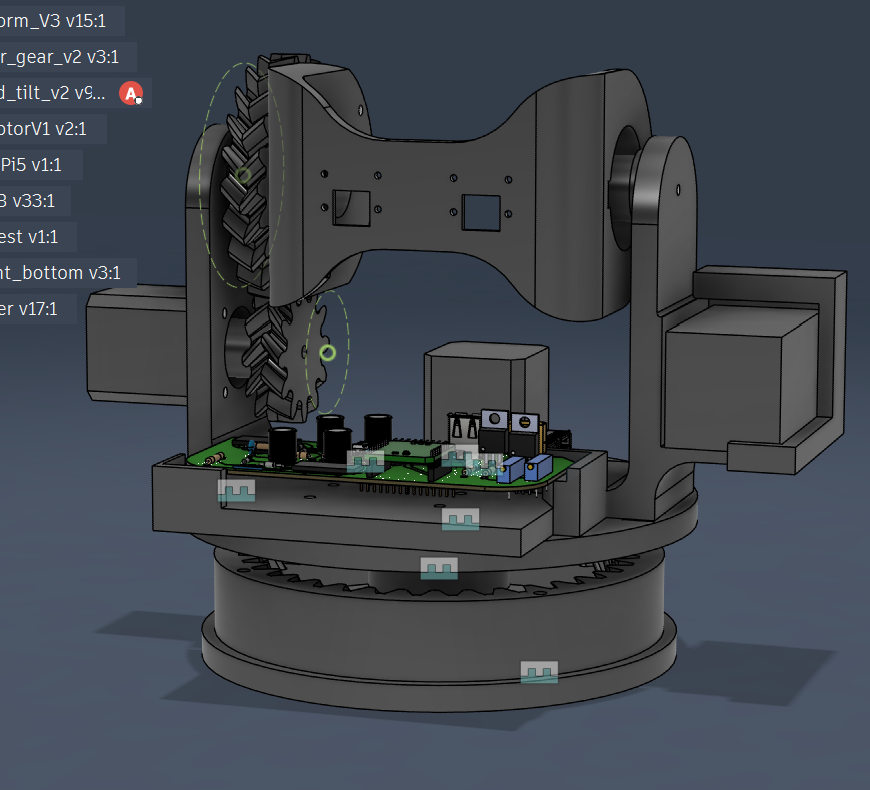
\includegraphics[width=\linewidth]{Figures/Andreas/3D Design/Full_assembly_V1.png}
        \caption{3D CAD design}
        \label{fig:full_assembli}
    \end{subfigure}
    \hfill
    \begin{subfigure}{0.45\linewidth}
        \centering
        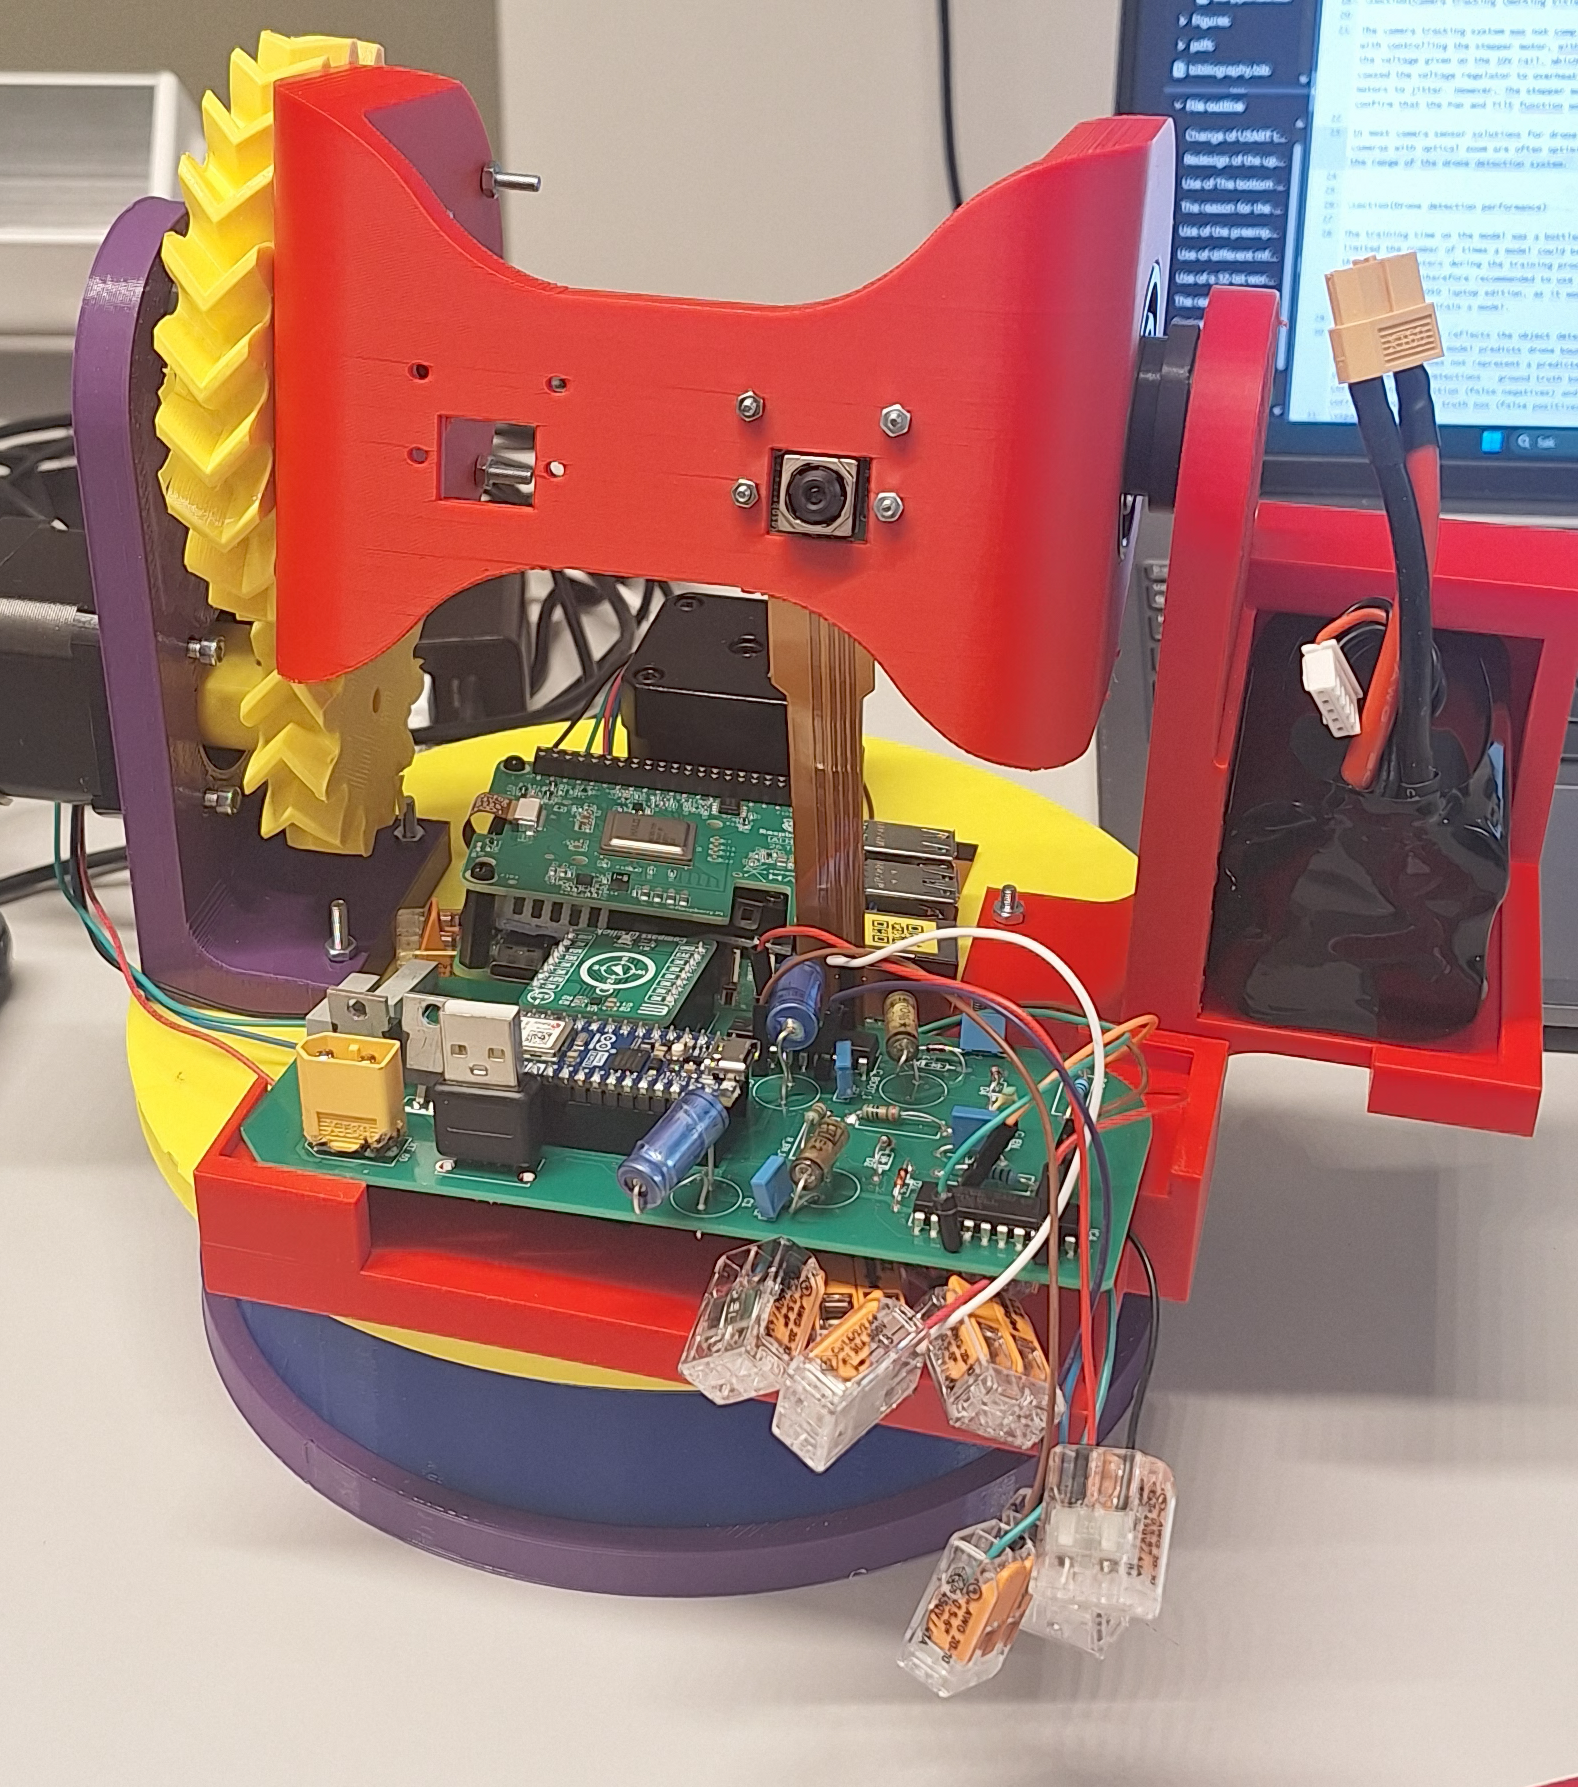
\includegraphics[width=\linewidth]{Figures/Andreas/3D Design/Full_print.png}
        \caption{Final printed version}
        \label{fig:full_print}
    \end{subfigure}
    \caption[3D design camera platform]{3D design camera platform}
    \label{fig:full_assembly_pair}
\end{figure}

The horizontal camera movement is controlled by a stepper motor connected to an 8 teeth gear which 
rotates around a 37 teeth track, giving it a full 360° rotation (fig: \ref{fig:pan_mechanism}). 
The gear ratio is $\frac{37}{8} = 4.625$, meaning the motor must complete 4.625 full rotations to 
rotate the platform 360°. Since each step of the stepper motor is 1.8°, one full motor rotation 
requires $\frac{360°}{1.8°} = 200$ steps, resulting in a total of $200 \times 4.625 = 925$ steps 
per full platform rotation, giving an angular resolution of $\frac{360°}{925} \approx 0.39°$ per step.

\begin{figure}[H]
    \centering
    \begin{subfigure}{0.45\linewidth}
        \centering
        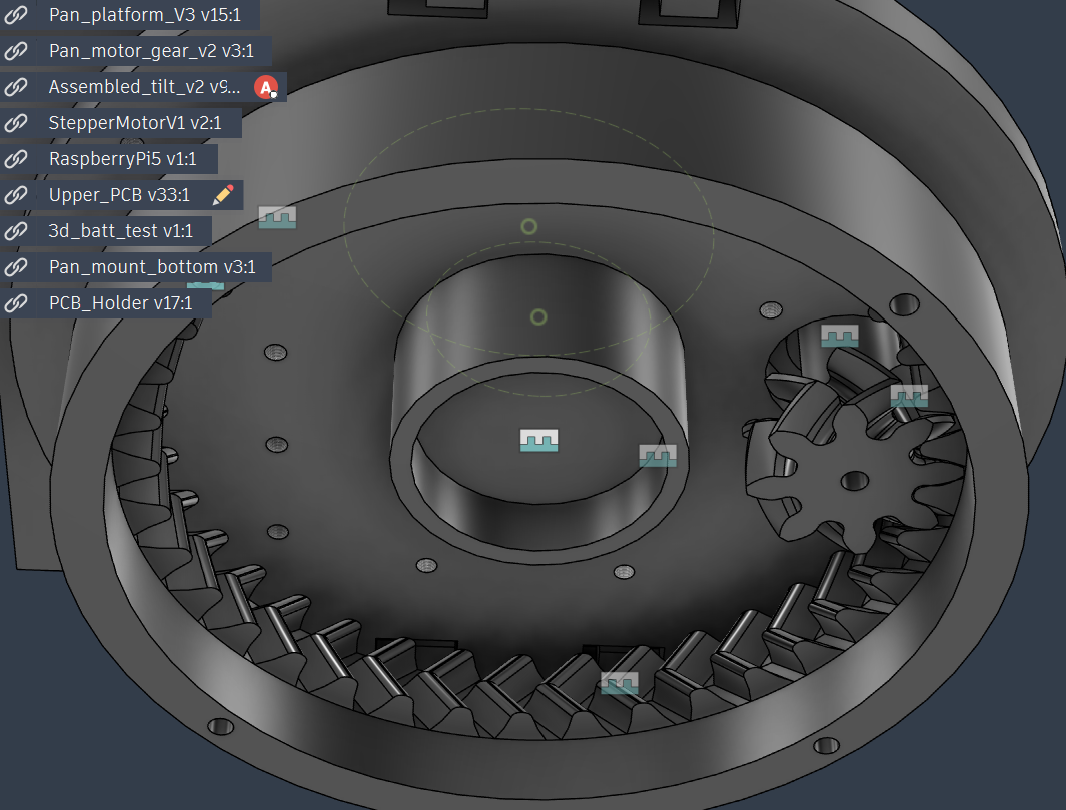
\includegraphics[width=\linewidth]{Figures/Andreas/3D Design/Pan_mechanism_V1.png}
        \caption{Screenshot from Fusion 360 of the pan mechanism.}
        \label{fig:pan_mechanism}
    \end{subfigure}
    \hfill
    \begin{subfigure}{0.35\linewidth}
        \centering
        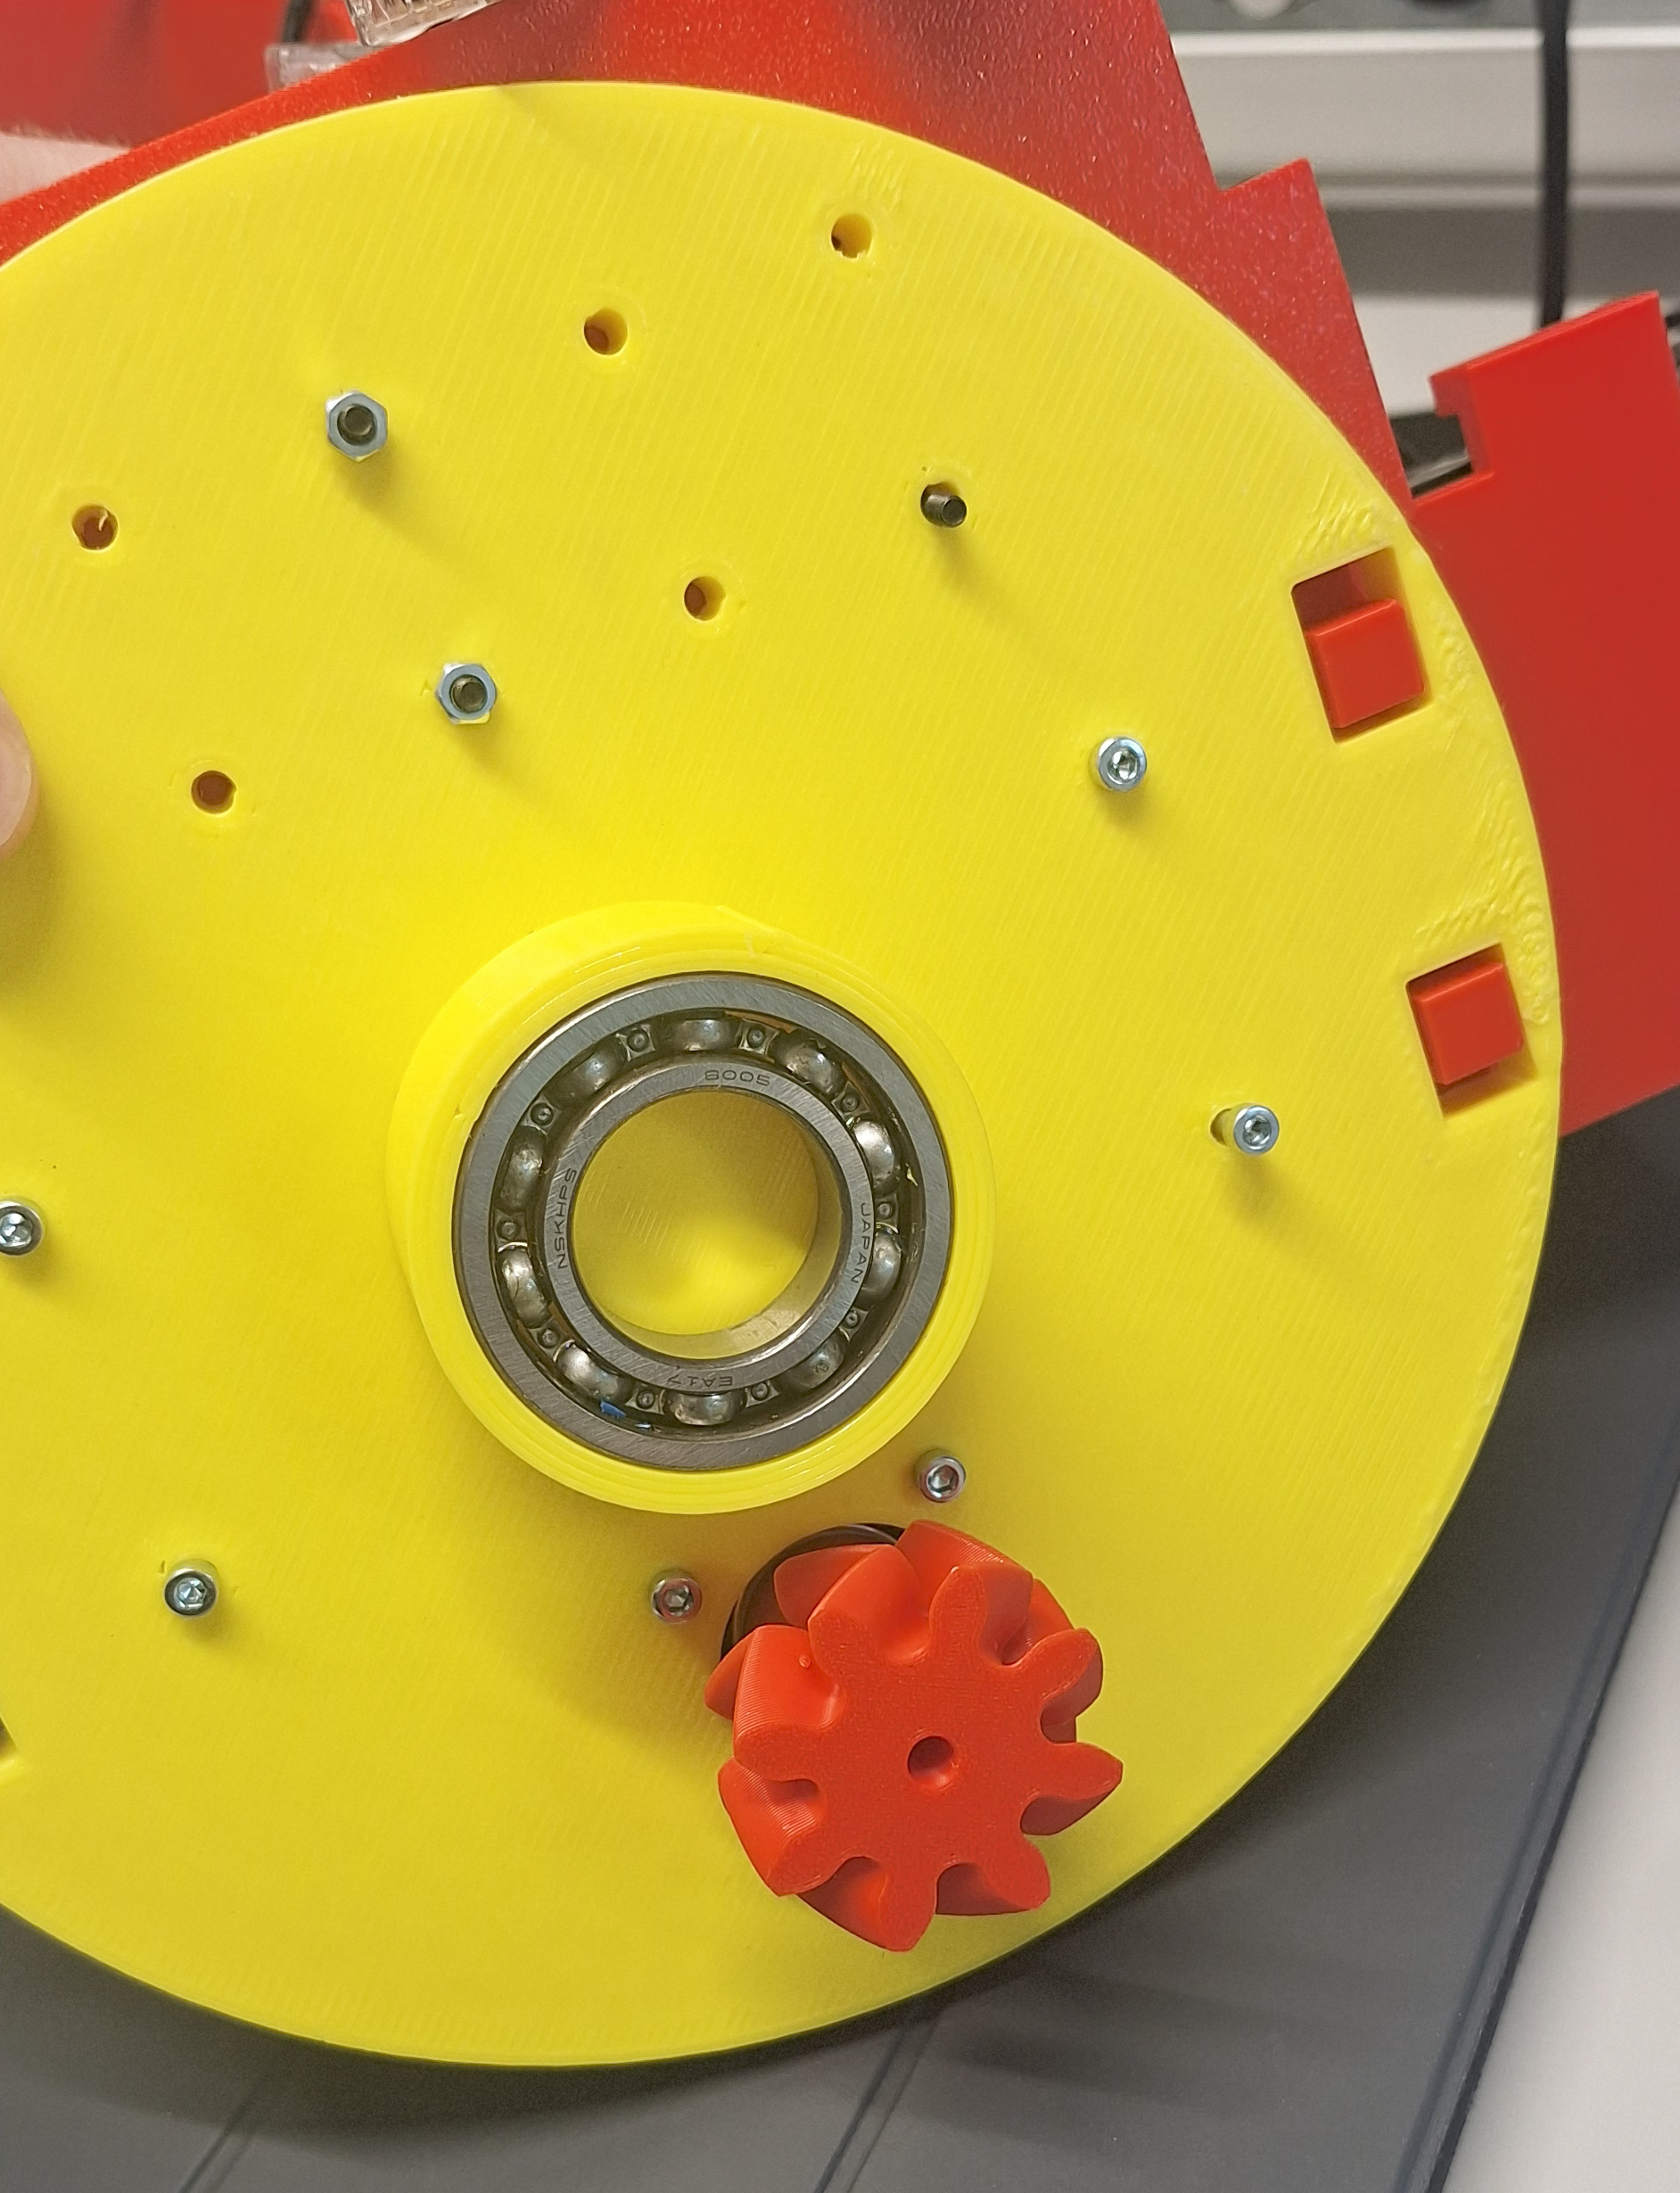
\includegraphics[width=\linewidth]{Figures/Andreas/3D Design/Bottom_ball_bearing.png}
        \caption{Image of the underside of the pan mechanism}
        \label{fig:bottom_ball_bearing}
    \end{subfigure}
    \caption[Pan mechanism]{Pan mechanism}
    \label{fig:pan_pair}
\end{figure}

The vertical camera movement is controlled by a stepper motor connected to a 12 teeth herringbone 
gear turning a larger 24 teeth herringbone gear (fig: \ref{fig:tilt_mechanism}). The gear ratio is 
$\frac{24}{12} = 2$, meaning the motor must complete 2 full rotations to rotate the camera 360°. 
With each step being 1.8°, one full motor rotation requires 200 steps, resulting in a total of 
$200 \times 2 = 400$ steps per full camera rotation, giving an angular resolution of 
$\frac{360°}{400} = 0.9°$ per step.

\begin{figure}[H]
    \centering
    \begin{subfigure}{0.45\linewidth}
        \centering
        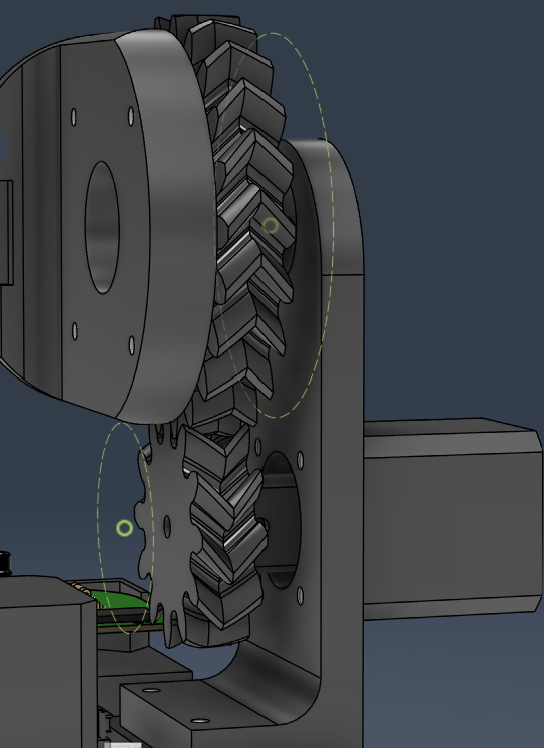
\includegraphics[width=\linewidth]{Figures/Andreas/3D Design/Tilt_mechanism_V1.png}
        \caption{Screenshot from Fusion 360 showing the tilt mechanism.}
        \label{fig:tilt_mechanism}
    \end{subfigure}
    \hfill
    \begin{subfigure}{0.45\linewidth}
        \centering
        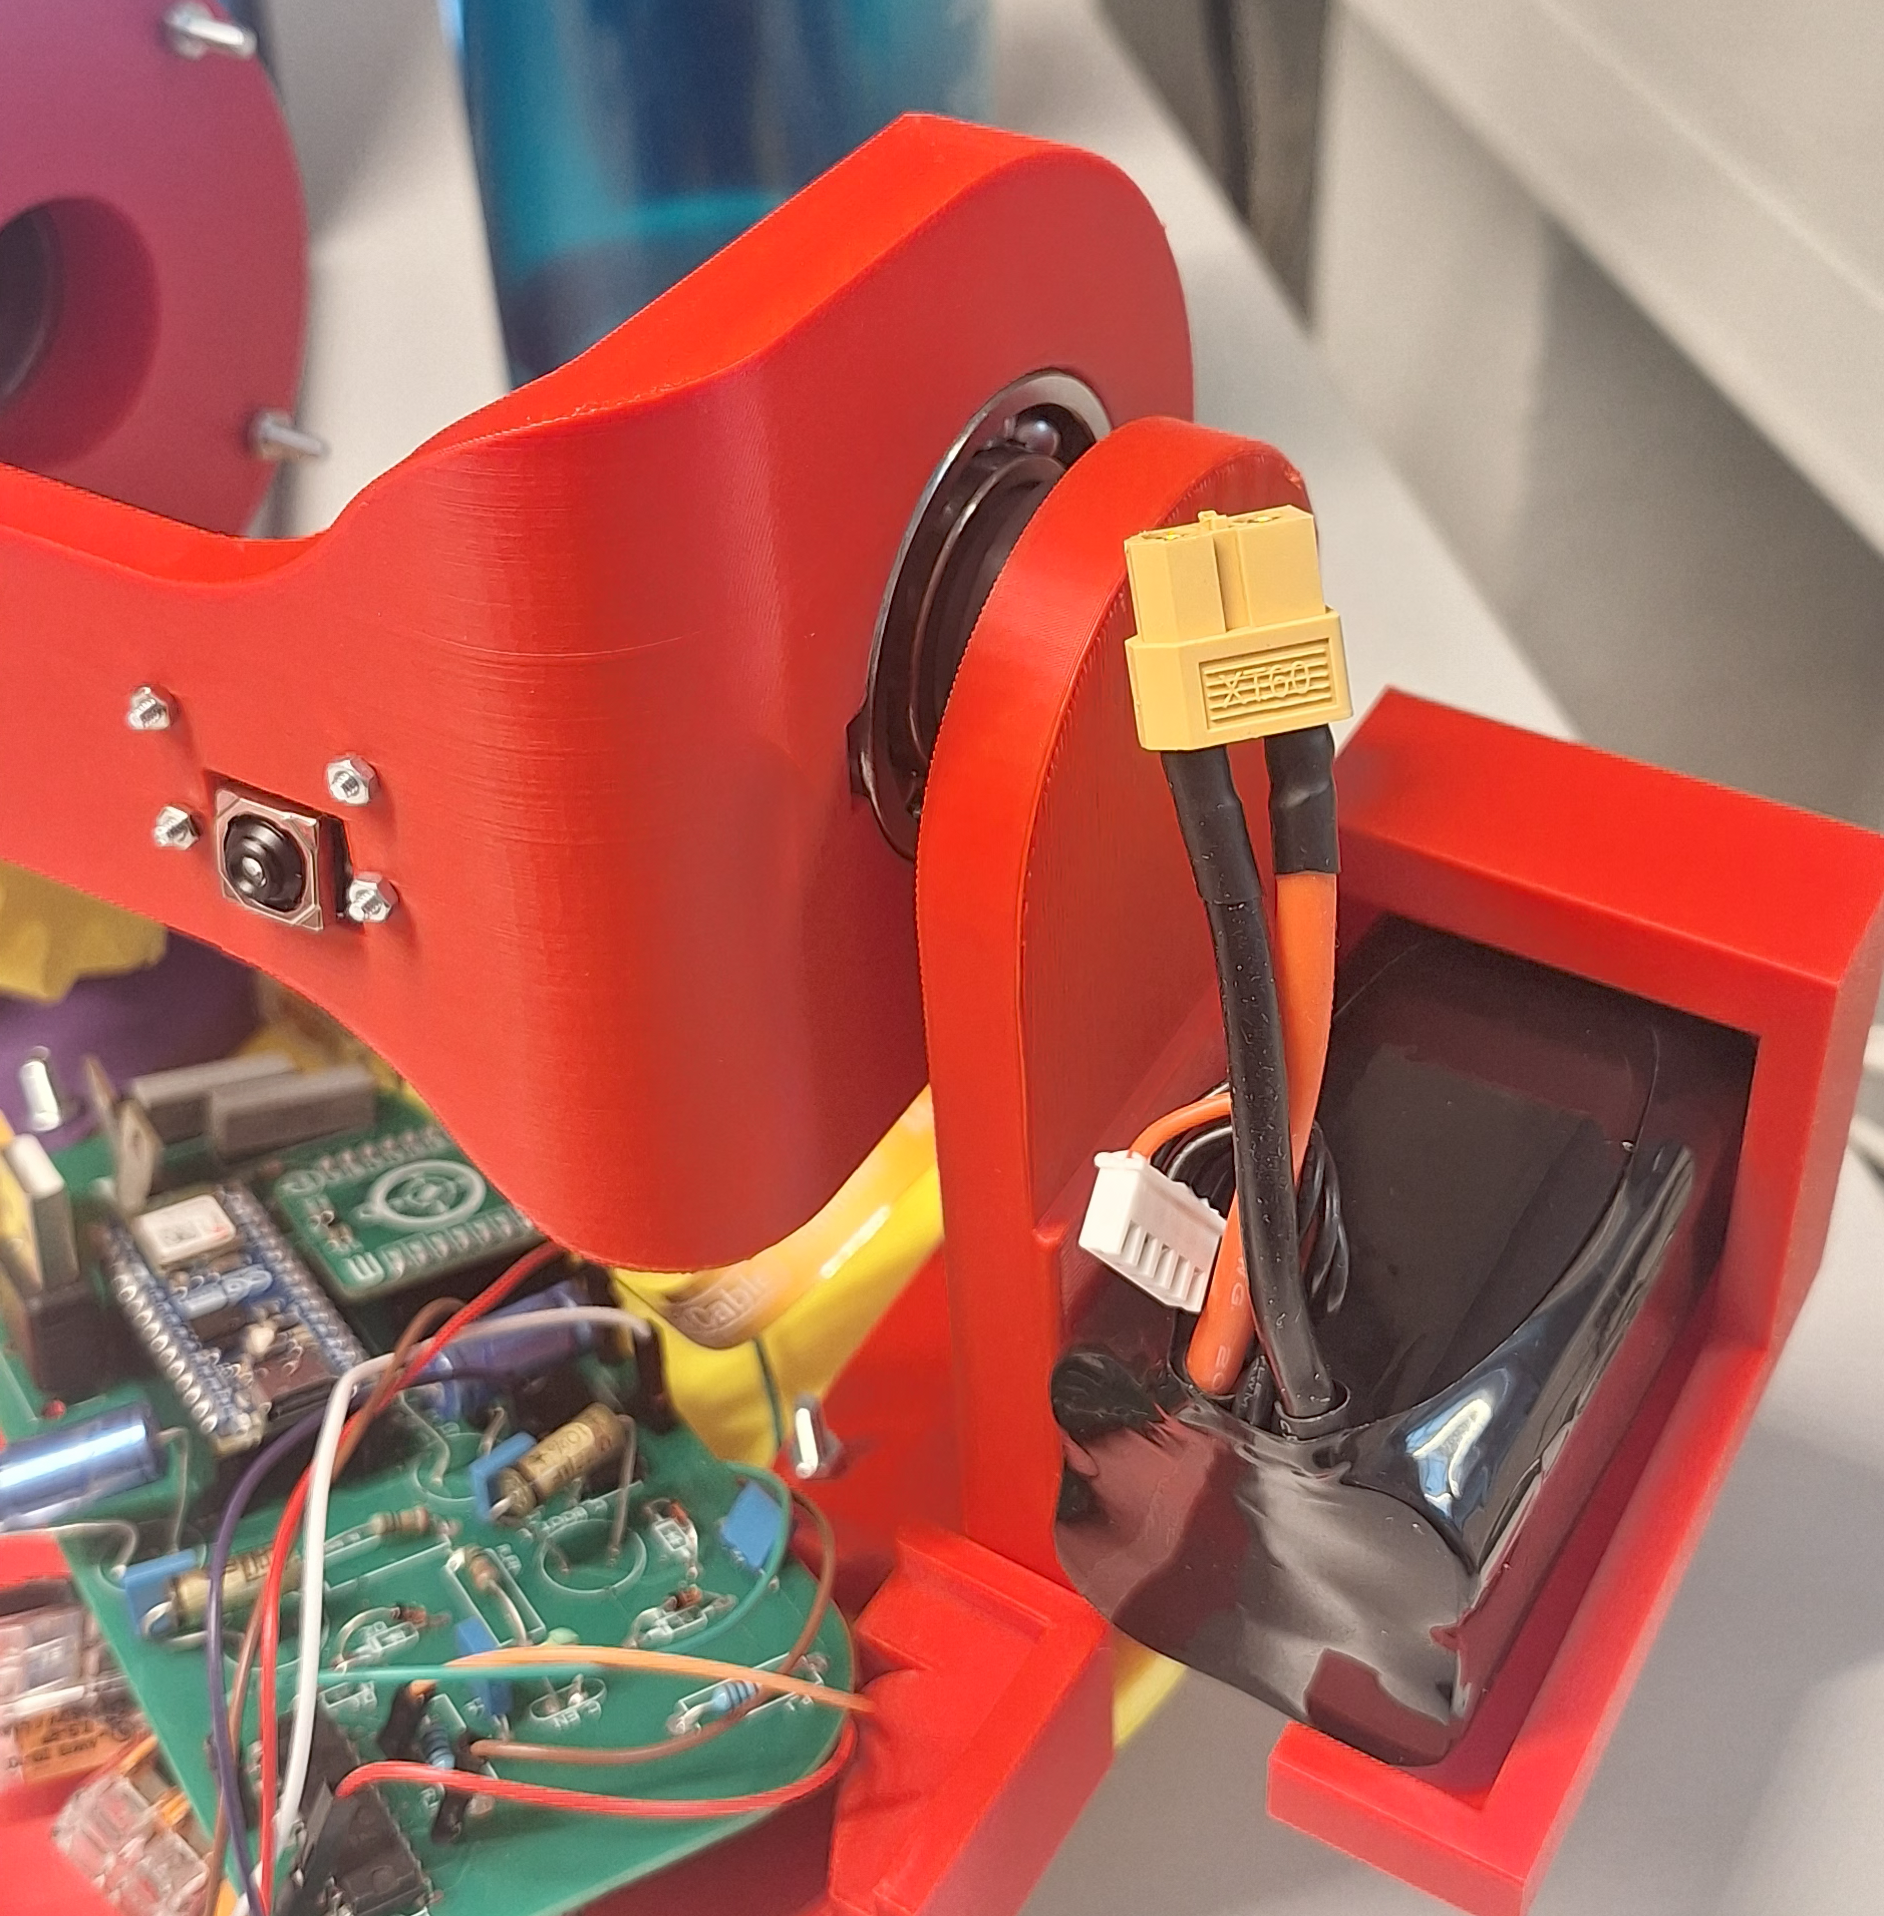
\includegraphics[width=\linewidth]{Figures/Andreas/3D Design/Side_ball_bearing.png}
        \caption{Ball bearing on the opposite side.}
        \label{fig:side_ball_bearing}
    \end{subfigure}
    \caption[Tilt mechanism]{Tilt mechanism}
    \label{fig:tilt_pair}
\end{figure}


\section{Hardware costs}

\begin{table}[h]
\centering
\caption{Equipment List with Prices for the system}
\label{tab:equipment}
\begin{tabular}{|l|l|r|}
\hline
\textbf{Component} & \textbf{Description} & \textbf{Price (NOK)} \\
\hline
Battery & Bronto 4S 5000mAh 21700 Li-Ion XT60 & 829 \\
\hline
Raspberry Pi 5 & 8 GB RAM & 2\,099 \\
\hline
Raspberry Pi AI HAT+ & AI accelerator add-on, 26 TOPS & 1\,499 \\
\hline
Raspberry Pi Camera Module & Camera for image capture & 509 \\
\hline
Stepper Motor $\times$2 & (2 units) & 962 \\
\hline
Compass & MikroElektronika Compass 6 Click, & 419 \\
\hline
Arduino Nano ESP32 & Microcontroller & 193 \\
\hline
Ball Bearing $\times$3 & ID 25\,mm, OD 47\,mm (3 units) & 240 \\
\hline 
STM32F413 & MCU for signal processing & 372 \\ 
\hline
PCB & Upper and bottom (has to buy 5x) & 700 \\ 
\hline
STEVAL-MIC002V1 & Microphone array (has 4 microphones) & 400 \\
\hline
L6205N & Motor controller (2x) & 200\\
\hline
Div electronics & resistors, voltage regulators etc. & 300 \\
\hline
\hline
\textbf{Camera Only total} & & \textbf{4\,517} \\
\hline
\textbf{Total} & & \textbf{8\,503} \\
\hline
\end{tabular}
\end{table}

\section{Acoustic Signal Acquisition and Analysis}
This section provides the explenation on how the acoustic signal was gathered and analysed to extract its spectrum and estimate the signals source of origin.


\subsection{Hardware Implementation for sound acquisition}
    \subsubsection{Microphone array and The expantion board} 
    The project uses an \href{https://www.st.com/resource/en/data_brief/steval-mic002v1.pdf}{\textbf{STEVAL-MIC002V1}} microphone array, which consists of four \href{https://www.st.com/resource/en/datasheet/mp34dt06j.pdf}{\textbf{MP34DT06J}} digital MEMS microhpones. The microphones are positioned as shown in Figure~\ref{fig:mics_on_the_tower}. Each microphone is placed 10 cm from the center of the platform along either the \textbf{X}-axis or \textbf{Y}-axis. All microphones are positioned in the same horizonatal plane, so the \textbf{Z}-coordinate, is set to zero for all micropohone positions. The position vector initialized in the \textbf{main.py} that describes the microphones position in relation to the platforms center, can be seen in Figure~\ref{fig:p_vector}. The microphones (beside the data pins) are connected to the \textbf{M1/2\_EXT} pins at the \href{https://www.st.com/en/evaluation-tools/x-nucleo-cca02m2.html}{\textbf{CCA02M2}} extantion board as seen in Figure~\ref{fig:CCA02M2_connection}. The CCA02M2 is used to supply the microphones with the clock signal and the 3.3V supply from the MCU. The board also allows to send the data signal from two microphones on the same line, by setting L/R pin high or low. That functionality was not used in the final stage of the project, as the data signal from the microphones is send directly to each microphone's own channel at the MCU, which directs the signal further to the connected DF. The extantion board is also used to send the PCM values from the MCU to the connected raspberry Pi or PC, through a micro usb which needs its own 5V supply, that is also provided by the connected MCU.

    \begin{figure}[h]
        \centering
        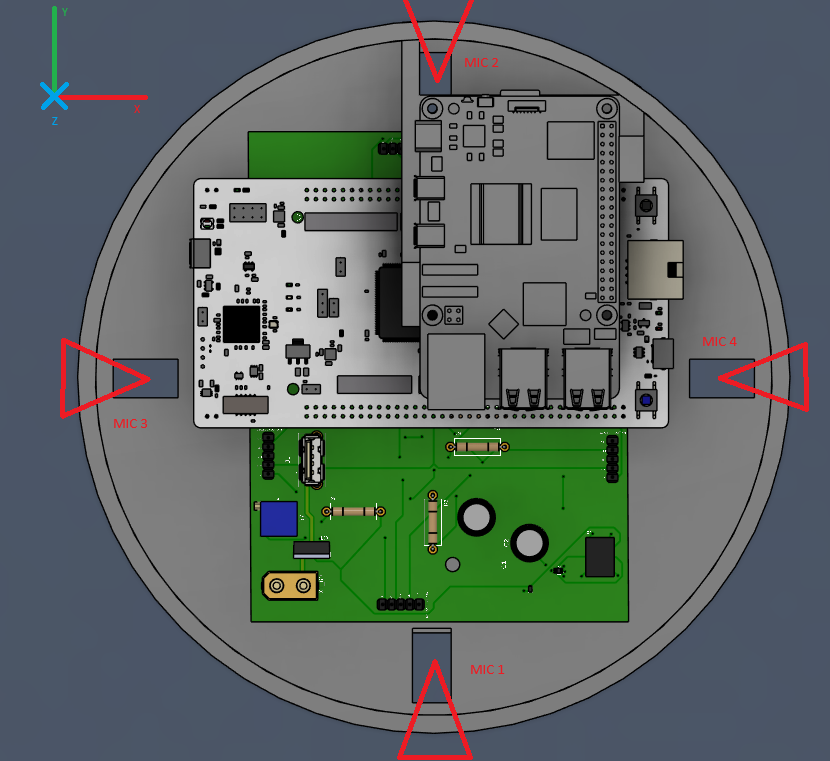
\includegraphics[width=0.75\linewidth]{Figures/mics.png}
        \caption[  The microphones placement]{The placement of the microhpones on the bottom part of the tower.}
        \label{fig:mics_on_the_tower}
    \end{figure}

    \begin{figure}[h]
        \centering
        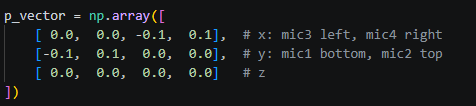
\includegraphics[width=0.5\linewidth]{Figures/p_vector.png}
        \caption[  P-vector]{P vector that represents the position of each microphone in relation to the platform center.}
        \label{fig:p_vector}
    \end{figure}

    \begin{figure}[h]
        \centering
        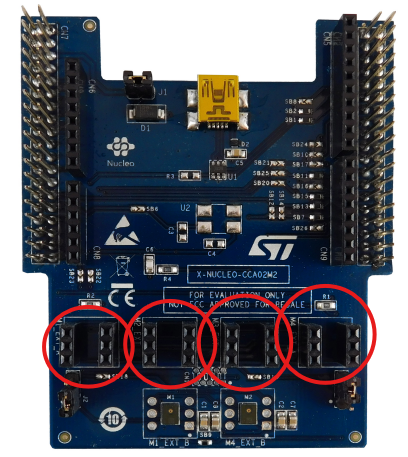
\includegraphics[width=0.5\linewidth]{Figures/cca02m2.png}
        \caption[  CCA02M2]{The CCA02M2 used in the project marked with outputs used for microphone connection. Source: \cite{x_nucleo_cca02m2_2019}.}
        \label{fig:CCA02M2_connection}
    \end{figure}

\newpage
    \subsubsection{STM32 configuration}
    The \href{https://www.st.com/en/microcontrollers-microprocessors/stm32f413zh.html#st_description_sec-nav-tab}{\textbf{F413ZH}}, is the MCU of STM32 model used in the final version of the project, and the reasoning for why this particular model was chosen, can be accessed in Section~\ref{sec:stm32_models_reasoning}.
    The STM32 was configured in CubeMX to use the I/O seen in Figure~\ref{fig:pinout_cubemx} and was phisically connected as in the Figure~\ref{}. The MCU supplies the extanstion board with the 3.3V and 5V signal, and sends the PCM data through it. The MCU, uses the peripherals seen in the Figure~\ref{fig:system_view_peripherals}, and some of them will be explained in the following sections.

    \begin{figure}[h]
        \centering
        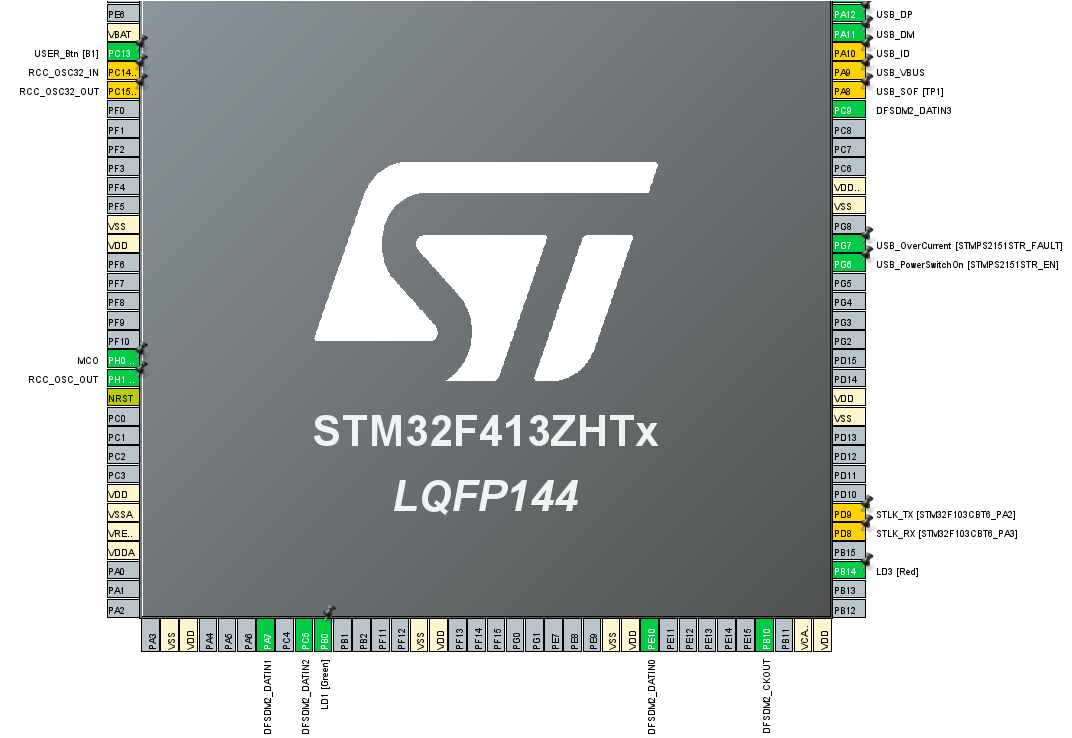
\includegraphics[width=0.75\linewidth]{Figures/pinout_cubemx.png}
        \caption[  STM32 pinout]{The pinout view of the STM32 F413ZH used in the project.}
        \label{fig:pinout_cubemx}
    \end{figure}


    \begin{figure}[h]
        \centering
        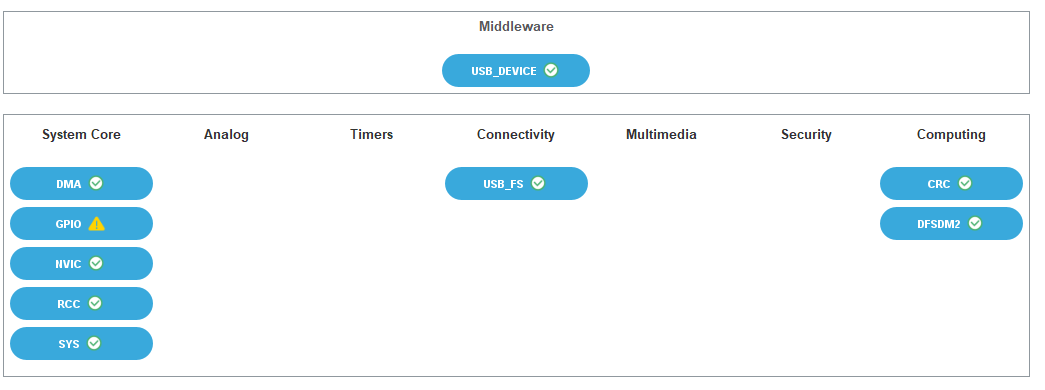
\includegraphics[width=0.5\linewidth]{Figures/system_view.png}
        \caption[  MCU peripherals]{System view of the MCUs peripherals}
        \label{fig:system_view_peripherals}
    \end{figure}
    \newpage
    
    \subsubsection{DFSDM configuration}
    The DFSDM was configured to be able to gather the acoustic signals from four microphones, hence the use of four separate channels as seen in Figure~\ref{fig:DFSDM2_modes}. But for the microphones to be able to send any data signal, they first have to be supplied by the clock signal, that they could use to adjust the data frequency to. The clock signal can be generated by the internal to the MCU clock as in Figure~\ref{fig:clock_dfsdm2}, which was set to 16Mhz. The clock signal is later reduced to around 2 Mhz and relied to the microphones by the \textbf{PB10} pin. 
    
    \begin{figure}[h]
        \centering
        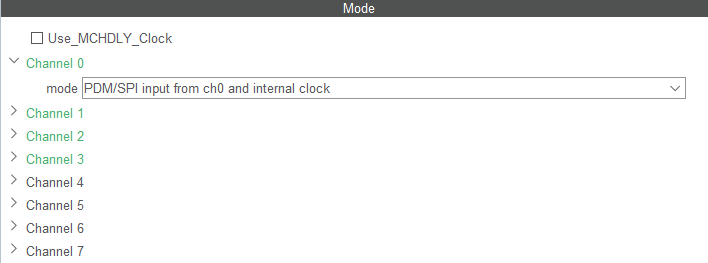
\includegraphics[width=0.5\linewidth]{Figures/modes_dfsdm.png}
        \caption[  DFSDM2 modes]{Modes in which the DFSM2 is configured}
        \label{fig:DFSDM2_modes}
    \end{figure}

    \begin{figure}[h]
        \centering
        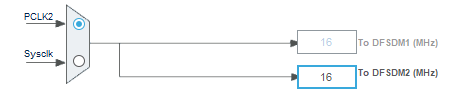
\includegraphics[width=0.5\linewidth]{Figures/DFSDM2_clock_config.png}
        \caption[  Clock for DFSDM2]{The clock frequency of the DFSDM2}
        \label{fig:clock_dfsdm2}
    \end{figure}
    \newpage

    

    If the signals from two microphones would be placed on the same line, type of the signal would have to be specified to either \textbf{SPI with falling edge} or \textbf{SPI with rising edge} as in Figure~\ref{fig:config_firstchannel} so that the signals could be properly deinterleaved. The channels watchdog can also be configured to monitor the signals behaviour, hovewer that functionality was not implememented in the final design.

    \begin{figure}[h]
        \centering
        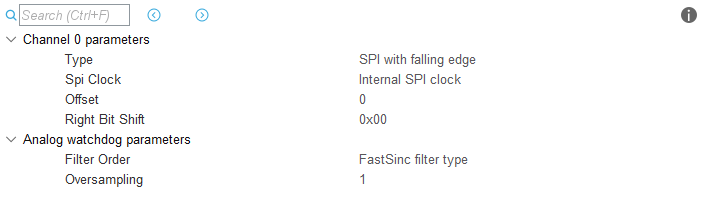
\includegraphics[width=0.5\linewidth]{Figures/channel0_config.png}
        \caption[  First DFSDM channel config]{Configuration of the first channel of the DFSDM.}
        \label{fig:config_firstchannel}
    \end{figure}
    \newpage

    Each filter was configured as in Figure~\ref{fig:config_filter_dfsdm}, where the main functions used are: the filter parameters of \textbf{Sinc Order} which was chosen to be of the 3th order, and the oversampling ratio \textbf{FOSR} of 32.  

    \begin{figure}[h]
        \centering
        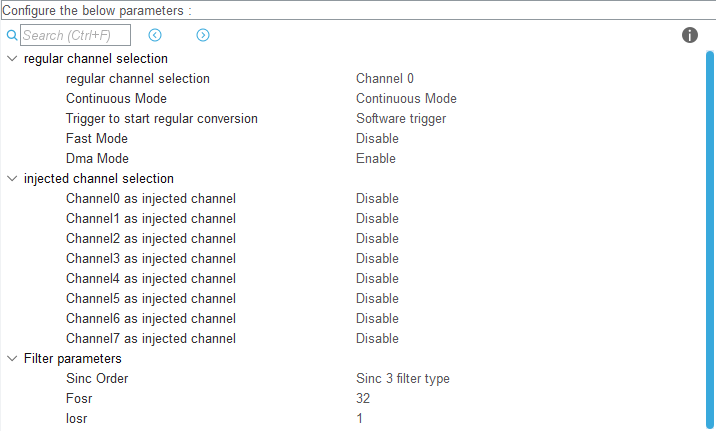
\includegraphics[width=0.5\linewidth]{Figures/filter_config_dfsdm.png}
        \caption[  Each filter config for DFSDM]{Configuration of each filter applied in DFSDM.}
        \label{fig:config_filter_dfsdm}
    \end{figure}

    The reason for the use of thesse values is that the third order sinc function, seamed to provide a reasonable balance between the sidelobe reduction and noise attenuation against the attenuation of the desired frequencies as seen in Figure~\ref{fig:mag_response_sinc}. The FOSR was selected to reduce the PDM bitstream to a lower PCM output rate while still maintaining a sampling frequnecy high enough to represent the relevant acoustic signal.  \\
 
    In the \textbf{main.c} in the STM32 project, the filter and channel handlers were declared as in Code~\ref{lst:dfsdm_filter_objects_declarations}, and later configured to operate togheter in the continous mode as in Code~\ref{lst:dfsdm_filter_config}, to insure that each channel is connected to the correct filter and that they sample and filter the microphone data correctly.\\

     \begin{lstlisting}[style=cstyle, caption={Declarations of the filter and channel objects}, label={lst:dfsdm_filter_objects_declarations}]
    DFSDM_Filter_HandleTypeDef hdfsdm2_filter0;
    DFSDM_Filter_HandleTypeDef hdfsdm2_filter1;
    DFSDM_Filter_HandleTypeDef hdfsdm2_filter2;
    DFSDM_Filter_HandleTypeDef hdfsdm2_filter3;
    DFSDM_Channel_HandleTypeDef hdfsdm2_channel0;
    DFSDM_Channel_HandleTypeDef hdfsdm2_channel1;
    DFSDM_Channel_HandleTypeDef hdfsdm2_channel2;
    DFSDM_Channel_HandleTypeDef hdfsdm2_channel3;
    \end{lstlisting}
    
    \begin{lstlisting}[style=cstyle, caption={Linking a DFSDM regular channel to a filter in continuous conversion mode}, label={lst:dfsdm_filter_config}]

if (HAL_DFSDM_FilterConfigRegChannel(&hdfsdm2_filter0,
                                       DFSDM_CHANNEL_0,
                                       DFSDM_CONTINUOUS_CONV_ON) != HAL_OK)
{
    Error_Handler();
}
    \end{lstlisting}
   \newpage
    \subsubsection{DMA buffering}
    The DMA was configured as in Figure~\ref{fig:dma_config}, to transfer the samples produced by the DFSDM peripheral to the internal memory of the MCU. Circular mode was used so that the DMA buffer could be reused continously during audio acquisition. When the end of the buffer is reached, the DMA controller starts writing the data from the begining of the buffer again, allowing for continous sampling. The Data samples were chosen to be stored as the 32-bit words in the DMA buffer, before the further processing and conversion. 
    
    \begin{figure}[h]
        \centering
        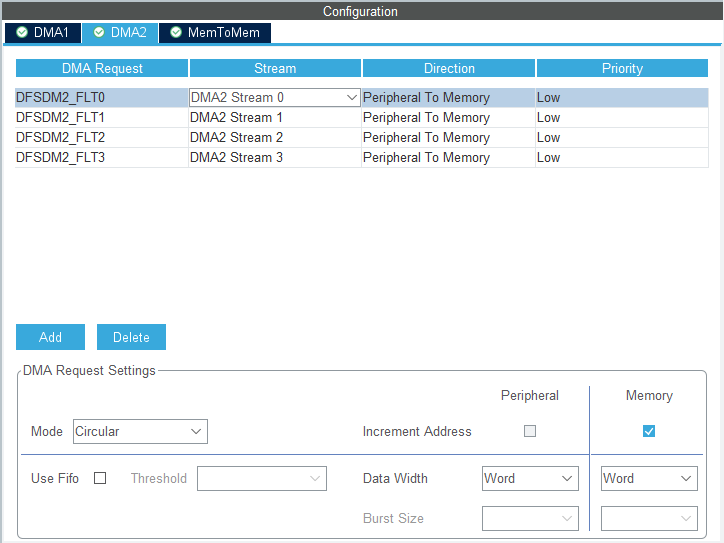
\includegraphics[width=0.5\linewidth]{Figures/dma_config.png}
        \caption[  DMA config]{Configuration of the DMA streams.}
        \label{fig:dma_config}
    \end{figure}

    The pcm buffers are declared as in the following Code~\ref{lst:PCM_buffer_declarations}. Each DFSDM filter has a dedicated DMA buffer declared as \textbf{int32\_t}, since the DFSDM peripheral outputs 32-bit samples. The buffer length is defined as twice the number of PCM samples used per half-buffer. This creates a double-buffer structrue, where one half of the buffer can be processed and send while the DMA is filling the other half. That is possible by setting the flags high for when the buffer is half full and completly full as shawn in Code~\ref{lst:callbacks_half_full}.
    The DMA handlers are declared as shawn in Code~\ref{lst:DMA_filter_obj}. These handlers are then used when starting the DFSDM regulator conversion with DMA as shawn in Code~\ref{lst:dfsdm_filter_to_pcm_buffer}. This connects each DFSDM filter output to its corresponding DMA buffer so that the converted samples are written to the memory. 
    
    \begin{lstlisting}[style=cstyle, caption={PCM buffers declaration}, label={lst:PCM_buffer_declarations}]
    
    #define PCM_SAMPLES_PER_HALF  16
    #define DFSDM_DMA_SAMPLES     (PCM_SAMPLES_PER_HALF * 2)
    
    static int32_t pcm0_dma[DFSDM_DMA_SAMPLES];
    static int32_t pcm1_dma[DFSDM_DMA_SAMPLES];
    static int32_t pcm2_dma[DFSDM_DMA_SAMPLES];
    static int32_t pcm3_dma[DFSDM_DMA_SAMPLES];
    \end{lstlisting}

    \begin{lstlisting}[style=cstyle, caption={Declaration of the DMA objects}, label={lst:DMA_filter_obj}]
    DMA_HandleTypeDef hdma_dfsdm2_flt0;
    DMA_HandleTypeDef hdma_dfsdm2_flt1;
    DMA_HandleTypeDef hdma_dfsdm2_flt2;
    DMA_HandleTypeDef hdma_dfsdm2_flt3;
    \end{lstlisting}
\newpage    
    \begin{lstlisting}[style=cstyle, caption={Connecting a DFSDM filter output to its dedicated DMA buffer}, label={lst:dfsdm_filter_to_pcm_buffer}]
     if (HAL_DFSDM_FilterRegularStart_DMA(&hdfsdm2_filter0, pcm0_dma, DFSDM_DMA_SAMPLES) != HAL_OK)
  {
      Error_Handler();
  }
  \end{lstlisting}

  \begin{lstlisting}[style=cstyle, caption={DMA half-complete and complete callbacks for DFSDM filter buffers. Generated by \cite{chatgpt2026}, although somewhat modified during the debuging process by adding the counter to each filter.}, label={lst:callbacks_half_full}]

    void HAL_DFSDM_FilterRegConvHalfCpltCallback(DFSDM_Filter_HandleTypeDef *hdfsdm_filter)
{
    if (hdfsdm_filter->Instance == DFSDM2_Filter0) { flt0_half_ready = 1; cb_half0++; }
    if (hdfsdm_filter->Instance == DFSDM2_Filter1) { flt1_half_ready = 1; cb_half1++; }
    if (hdfsdm_filter->Instance == DFSDM2_Filter2) { flt2_half_ready = 1; cb_half2++; }
    if (hdfsdm_filter->Instance == DFSDM2_Filter3) { flt3_half_ready = 1; cb_half3++; }
}

void HAL_DFSDM_FilterRegConvCpltCallback(DFSDM_Filter_HandleTypeDef *hdfsdm_filter)
{
    if (hdfsdm_filter->Instance == DFSDM2_Filter0) { flt0_full_ready = 1; cb_full0++; }
    if (hdfsdm_filter->Instance == DFSDM2_Filter1) { flt1_full_ready = 1; cb_full1++; }
    if (hdfsdm_filter->Instance == DFSDM2_Filter2) { flt2_full_ready = 1; cb_full2++; }
    if (hdfsdm_filter->Instance == DFSDM2_Filter3) { flt3_full_ready = 1; cb_full3++; }
}

    \end{lstlisting}
    
    \subsubsection{USB CDC FS communication}
    The USB CDC FS was used to transfer the PCM samples from the MCU to the PC. The USB had to be provided a 48 Mhz clock signal as shawn in Figure~\ref{fig:clock_usb}, so that the PC could recognize the transfered data. 
    
    \begin{figure}[h]
        \centering
        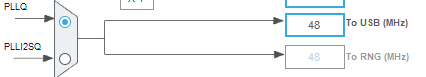
\includegraphics[width=0.5\linewidth]{Figures/usb_clock_config.png}
        \caption[  USB clock frequency]{The clock frequency of the USB}
        \label{fig:clock_usb}
    \end{figure}

    To make it possible for the receiver script to detect the start of each data packet, a two-byte synchronization word was added before the audio payload, as shown in Code~\ref{lst:usb_sync}.\\

    \begin{lstlisting}[style=cstyle, caption={Bytes used for syncing the data packages}, label={lst:usb_sync}]
    #define USB_SYNC_0            0x5A
    #define USB_SYNC_1            0xA5
    \end{lstlisting}

    \newpage
    The PCM values in the two-byte format are transfered to the receiver script by using the \textbf{PackAndSendFrame} function in \textbf{main.c} of the MCU program. The function is called in the \textbf{While} loop visible in the Code~\ref{lst:while_loop_c}, when all of the filter buffers were either half-full og completly full. The function itself can be seen in Code~\ref{lst:pack_and_send}, and its main task is to transfer 16 samples from each DMA filter buffer to a separate container, and place it into a frame. The packed frame is later send through the \textbf{CDC\_Transmit\_FS} method to the receiver script.\\

\begin{lstlisting}[style=cstyle, caption={Main loop for checking DMA buffer readiness and transmitting audio frames}, label={lst:while_loop_c}]
     while (1)
  {
	      if (flt0_half_ready && flt1_half_ready && flt2_half_ready && flt3_half_ready)
	      {
	          flt0_half_ready = 0;
	          flt1_half_ready = 0;
	          flt2_half_ready = 0;
	          flt3_half_ready = 0;
	          PackAndSendFrame(0);
	      }
	      if (flt0_full_ready && flt1_full_ready && flt2_full_ready && flt3_full_ready)
	      {
	    	  flt0_full_ready = 0;
	    	  flt1_full_ready = 0;
	    	  flt2_full_ready = 0;
	    	  flt3_full_ready = 0;
	          PackAndSendFrame(1);
	      }
  }
\end{lstlisting}
    \begin{lstlisting}[style=cstyle, caption={Function for packing and sending each frame, generated by \cite{chatgpt2026}}, label={lst:pack_and_send}]
    static void PackAndSendFrame(uint8_t half_index)
{
    uint32_t start = (half_index == 0) ? 0 : PCM_SAMPLES_PER_HALF;
    usb_frame[0] = USB_SYNC_0;
    usb_frame[1] = USB_SYNC_1;
    uint32_t j = 2;
    for (uint32_t i = 0; i < PCM_SAMPLES_PER_HALF; i++)
    {
        int16_t mic0 = DFSDM32_to_PCM16(pcm0_dma[start + i]);
        int16_t mic1 = DFSDM32_to_PCM16(pcm1_dma[start + i]);
        int16_t mic2 = DFSDM32_to_PCM16(pcm2_dma[start + i]);
        int16_t mic3 = DFSDM32_to_PCM16(pcm3_dma[start + i]);
        
        usb_frame[j++] = (uint8_t)(mic0 & 0xFF);
        usb_frame[j++] = (uint8_t)((mic0 >> 8) & 0xFF);
        usb_frame[j++] = (uint8_t)(mic1 & 0xFF);
        usb_frame[j++] = (uint8_t)((mic1 >> 8) & 0xFF);
        usb_frame[j++] = (uint8_t)(mic2 & 0xFF);
        usb_frame[j++] = (uint8_t)((mic2 >> 8) & 0xFF);
        usb_frame[j++] = (uint8_t)(mic3 & 0xFF);
        usb_frame[j++] = (uint8_t)((mic3 >> 8) & 0xFF);
    }
    CDC_Transmit_FS(usb_frame, sizeof(usb_frame));
}
void CDC_TransmitCplt_FS(uint8_t *Buf, uint32_t *Len, uint8_t epnum)
{
    (void)Buf;
    (void)Len;
    (void)epnum;
    usb_tx_busy = 0;
}
\end{lstlisting}
\subsection{Data Acquisition and Communication}
The data from the microhpones was transmitted in the PDM format, and acquired by the DFSDM peripheral. After filtering and decimatiion in the DFSDM, the resulting PCM samples were transmitted to the PC through USB CDC. 

    \subsubsection{PDM input from digital MEMS microphones}
    The digital MEMS microhpones output a PDM bitstream, where the data rate is controlled by the clock signal applied to  the \textbf{CLK} pin. In the project, the clock signal was generated by the DFSDM peripheral and set to 2 Mhz, which is right between the necessery signal frequency of 1.2 Mhz to 3.25 Mhz according to \cite{st_mp34dt06j_2021}. The resulting PDM stream varies according to the acoustic pressure measured by each microphone and was used as the input to the DFSDM channels. 

    \subsubsection{PDM to PCM conversion with DFSDM}
    The PDM samples are converted to PCM format by the DFSDM peripheral, which uses the sinc filter of the 3rd order and decimates the values by the ratio of 32. The newly converted samples are then stored in a 32-bit word, which are furtherly converted to the \textbf{int16\_t} format to reduce the maximal value of each sample as seen in Code~\ref{lst:pack_and_send}.   
    
    \begin{lstlisting}[style=cstyle, caption={Limiting the shifted DFSDM output to the valid signed 16-bit PCM range. Generated by \cite{chatgpt2026}.}, label={lst:pack_and_send}]
    static int16_t DFSDM32_to_PCM16(int32_t x)
    {
        x >>= 8;
    
        if (x > 32767)  x = 32767;
        if (x < -32768) x = -32768;
        return (int16_t)x;
    }
    \end{lstlisting}
    \subsubsection{PCM samples}
    Each microphone is expected to provide 16 PCM samples per iteration after the conversion from PDM to PCM. The reason for that, is the earlier application of SAI and pdm2pcm library, where the user had to specify the number of output samples and the decimation rate. Where by using the decimation rate of 64, and the PCM samples number of 16 togheter with the clock signal, the user was then able reach the desired Fs of around 24Khz per second. So to not chagne the later pipeline involving the receiver script, the number of samples was not changed.  

    
    \newpage
    \subsubsection{PCM sample format sent by the usb}
        \label{sec:PCM_sample_format_sent_by_usb}
        The MCU sends the PCM samples in frames of the format that can be seen in Table~\ref{tab:usb_frame_structure}. Each frame starts with a two byte synchonization word, followed  by the adio payload. The payload contains 16 PCM samples from each mirophone and since each PCM sample is stored as an \textbf{int16\_t} value, each sample requires 2 bytes. That gives 32 data bytes per microphone channel and 128 bytes of the data payload in total. By adding the two sync bytes, the total frame length becomes 130 bytes. 
        
\begin{table}[h]
\centering
\caption{USB frame structure}
\label{tab:usb_frame_structure}
\begin{tabular}{|c|c|c|c|}
\hline
\textbf{Field} & \textbf{Size} & \textbf{Content} & \textbf{Description} \\
\hline
Sync word & 2 bytes & 0x5A 0xA5 & Marks the start of a new frame \\
\hline
Audio payload & $16 \times 4 \times 2$ bytes & PCM samples & 16 samples per microphone \\
\hline
Total frame & 130 bytes & Sync + payload & Complete USB frame sent to Python \\
\hline
\end{tabular}
\end{table}

\subsection{The main python program for the signal processing}
The part of the system responsible for the signal processing of the acoustic signal, sound source estimation and the feature extraction is controlled by the \textbf{main.py} file found in the \textbf{Drone\_detection\_porgram\_bachelor/} folder. The program pipeline can be seen in the Figure~\ref{fig:main_flowchart}. The program initializes the following objects Code~\ref{lst:init_main_py}, which are responsible for receiving the microphone signal, estimating the source of the incoming signal and also extraction of the features present in the signal, that can be later used in the ML based classifier.

\begin{lstlisting}[style=pythonstyle, caption={Initialization of the objects used in the main.py}, label={lst:init_main_py}]
from receivers.stm32_usb_receiver import STM32UsbReceiver
from dataset_tools.create_wav_file import WavCreation
from features.mfcc_extraction import  MFCCExtractor
from features.feature_exporter import FeatureExporter
from features.feature_visualizer import FeatureVisualizer
from debug.stm32_usb_receiver_debug_tools import ReceiverDebug
from gcc.gcc_processor import GCCProcessor
from gcc.doa_estimator import DOAEstimator
from gcc.doa_visualizer import DOAVisualizer

receiver = STM32UsbReceiver()
wav_conversion = WavCreation()
mfcc_extractor = MFCCExtractor()
mfcc_exporter = FeatureExporter(extractor=mfcc_extractor)
mfcc_visualizer = FeatureVisualizer(extractor=mfcc_extractor)
gcc_processor = GCCProcessor()
doa_estimator = DOAEstimator(p_vector, gcc_processor)
doa_visualizer = DOAVisualizer()
#debug 
receiver_debug = ReceiverDebug(receiver=receiver)
\end{lstlisting}

\newpage
\begin{figure}[h]
    \centering
    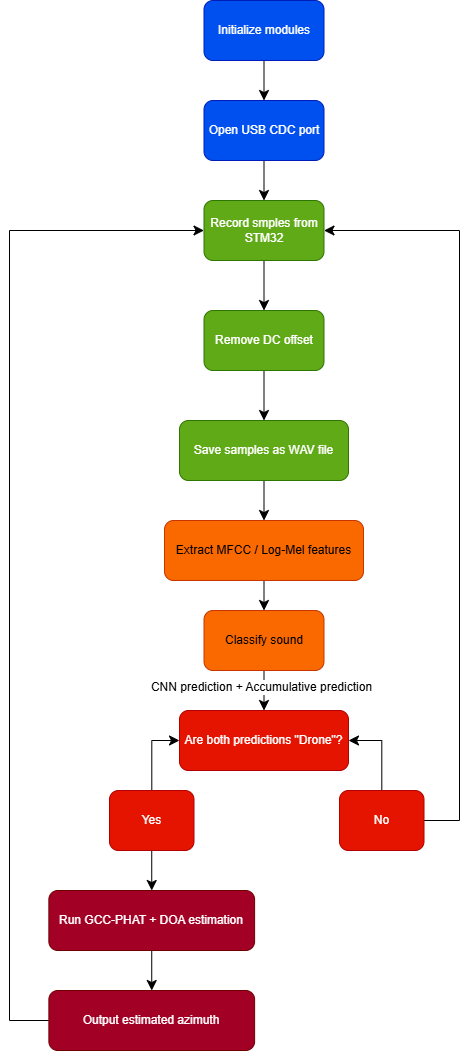
\includegraphics[width=0.5\linewidth]{Figures/main_program.drawio.png}
    \caption[  Flowchart-main program for audio]{Flowchart for the main program for audio processing }
    \label{fig:main_flowchart}
\end{figure}
The program runs continuously, as it is based on a while loop, which can be modified to either run infinitely, or for a set number of iterations. The program loop used during the system testing can be seen in Code~\ref{lst:while_main}.
\newpage
\begin{lstlisting}[style=pythonstyle, caption={The main program loop for sound detection and classification}, label={lst:while_main}]
while Run:
    i+=1
    samples = receiver.record() # record the data sent by the stm32
    # test DC offset 
    samples= samples.astype(np.float32)
    samples = samples - np.mean(samples)

    wav_conversion.convert_into_wav(samples, receive_time=receiver.start_time, duration= receiver.duration_sec) # convert the samples into a wav format
    receiver_debug.debug_export(plot_debug=True)

    # features 
    features = mfcc_extractor.extract_features(audio_file=f"debug_figures/04_05_drone_test_riktig_plassering/mic_recording{receiver.start_time}.wav") # extract features such as mfcc, delta, delta2, log_mel_spec etc
    mfcc_exporter.df_features() # export the features into a df
    # adds a lot of overhead, comment out during live testing
    #mfcc_visualizer.mel_spectrogram(receiver.start_time)
    #mfcc_visualizer.spectrogram(receiver.start_time)
    
    # Sound classification
    cnn_predict = cnn_model.cnn_predict(f"debug_figures/04_05_drone_test_riktig_plassering/mic_recording{receiver.start_time}.wav") #Fix, add permanent non debug location
    accumulative_predict = accumulative_model.acum_predict(features)
    
    if cnn_predict == "Drone" and accumulative_predict == "Drone":
        # Direction
        gcc_array = gcc_processor.process_signal(samples, mfcc_extractor.fs)
        doa_estimator.set_gcc_array(gcc_array)
        doa_estimator.estimate_DOA()
        print(f"Azimuth this iteration is: {doa_estimator.estimated_azimuth_deg}")
        print(f"Iteration: {i}")
        # adds a lot of overhead, comment out during live testing
        #doa_visualizer.visualize_doa(doa_estimator.estimated_azimuth_deg, doa_estimator.estimated_azimuth_rad, #receiver.start_time)
        
    if i == 45: # allows for 45 iterations, before the program terminates
        Run = False   
    # debug 
    print(f"CNN prediction: {cnn_predict}")
    print(f"Accumulative prediction: {accumulative_predict}")
    
    if debug_mfcc:
        mfcc_visualizer.plot_signal_time()
        mfcc_visualizer.spectrogram()
        mfcc_visualizer.mel_spectrogram()
        Run = False
    if debug_stm32:
        receiver_debug.debug_export(plot_debug=True)
        Run = False 
\end{lstlisting}

During each iteration, the new samples are measured, by calling the \textbf{record} member function of the receiver object. Then the DC offset is subtracted from the signal, to center the signal around zero. The measured signal has to be converted into a wav sound file, which is the needed signal format for the MFCC extraction class. The signal features are then extracted by using the \textbf{extract\_features} from the MFCC extractor type object, which will later be send to the ML classifier to decide what kind of the object is producing the sound. But before that the direction of the source signal will be estimated, and the program will then determine based on the classifiers output, to either keep the estimated azimuth or to find a new one that correclty represents drone signal source. The program uses also some debug functions, which were extensively used during the testing stage of the project.  


\subsection{Python receiving and preprocessing}
The PCM signal transmitted by the MCU to the host computer is first handled by a Python receiving module, placed in the \textbf{Drone\_detection\_porgram\_bachelor/receivers} folder, called \textbf{stm32\_usb\_receiver.py}. The module decodes the incoming USB frames and prepers the microphone singal for the later processing stages such as direction estimation and feature extraction. 

    \subsubsection{USB CDC receiver}
    The receiver object was initialized using the configuration shown in Table~\ref{tab:receiver_config}. The parameters are used to define the USB port, the expected synchronization word, the number of microphones, samples per microphone, the duration time of the recording and the number of expected bytes in the frame.

    \begin{table}[h]
\centering
\caption{Configuration parameters used by the STM32 USB receiver}
\label{tab:receiver_config}
\begin{tabular}{|c|c|c|}
\hline
\textbf{Parameter} & \textbf{Value} & \textbf{Description} \\
\hline
\texttt{port} & \texttt{COM16} & USB CDC port used on Windows \\
\hline
\texttt{sync} & \texttt{0x5A 0xA5} & Two-byte synchronization word \\
\hline
\texttt{channels} & 4 & Number of microphone channels \\
\hline
\texttt{frame\_samples} & 16 & Number of samples per microphone in each frame \\
\hline
\texttt{duration\_sec} & 1 & Recording duration for each iteration \\
\hline
\texttt{frame\_bytes} & 130 & Expected size of one complete USB frame \\
\hline
\end{tabular}
\end{table}
    The receiver class contains methods for opening and closing the USB CDC port, but the main processing is performed by the \textbf{record()} method which can be seen in Code~\ref{lst:record_method}. 
    \newpage
    \begin{lstlisting}[style=pythonstyle, caption={Record the signal method. Was originally generated by \cite{chatgpt2026}, but was modified during the debuging process}, label={lst:record_method}]
    def record(self):
        # remove old data, initiate a temp buffer
        if self.port_opened:
            self.ser.reset_input_buffer() 
            rx_buf = bytearray()

            print("Recording..")
            self.start_time = time.time()
            self.samples = [[] for _ in range(self.channels)] #reset the samples before recording any new values
            
            while time.time() - self.start_time < self.duration_sec :
                data = self.ser.read(512) # 512 bytes
                
                if not data:
                    continue
                rx_buf.extend(data) # adds data to rx_buf

                while True:
                    sync_idx = rx_buf.find(self.sync) 

                    if sync_idx < 0: # if sync was not in the buffer
                        # keep the last byte in case sync 2 bytes are divided between packages
                        rx_buf = rx_buf[-1:]
                        break

                    if len(rx_buf) < sync_idx + self.frame_bytes:
                        # if the length of data is smaller then the expected frame length plus sync bytes
                        break

                    frame = rx_buf[sync_idx + 2 : sync_idx + self.frame_bytes]
                    rx_buf = rx_buf[sync_idx + self.frame_bytes:] # removes the processed frame 

                    samples = np.frombuffer(frame,dtype=np.int16) # interpret as signed int16
                    
                    # vectorized 
                    samples = samples.reshape(-1, self.channels)
                    self.samples = [np.concatenate((self.samples[ch], samples[:,ch])) for ch in range(self.channels)]
    
            return np.array(self.samples)

        else:
            raise RuntimeError("THE PORT WAS NOT OPENED! Use open_port().")

        \end{lstlisting}
    
     The method after opening the port, zeroes out the samples for each channel connected to the object, insuring that only the data from the current iteration will be processed. The data is being gathered for a default duration of 1 second, during which the package is controlled for the sync bytes. If the sync bytes are not present in the package, the receiver keeps the last byte and waits for more of the incoming data, in case the sync word was splitt between two reads. If the sync bytes are found, but the buffer does not yet contain the complete 130 bytes frame, the receiver also waits for more data before processing the frame. After the complete frame has been extracted, the sync bytes are removed, and the remaining data is then stored in the \textbf{frame} container. In its current format, the payload is still just a byte-string, which has to be interpreted as 16-bit integer values to reconstruct the PCM values. Since the payload sent from the MCU is interleaved, each sample index contains one sample from each microphone in the order mic0, mic1, mic2 and mic3. The payload is therefore reshaped into four colums, where each represents an independent microphone signal.   
    
    \subsubsection{DC offset removal}
    The DC offset removal was conducted in the \textbf{main.py} in Code~\ref{lst:DC_Offset}, by converting the values inside of the \textbf{samples} containter into the \textbf{float32} format to insure that the function \textbf{np.mean()} can be applied. Then the mean value of the signal was subtracted from the samples. This removes the value that the signal is circulating around as seen in Figure~\ref{fig:DC_offset} and effectively centers the values around zero . 

    \begin{lstlisting}[style=pythonstyle, caption={DC offset romoval}, label={lst:DC_Offset}]
    # test DC offset 
    samples= samples.astype(np.float32)
    samples = samples - np.mean(samples)
    \end{lstlisting}

    \begin{figure}[h]
    \centering
    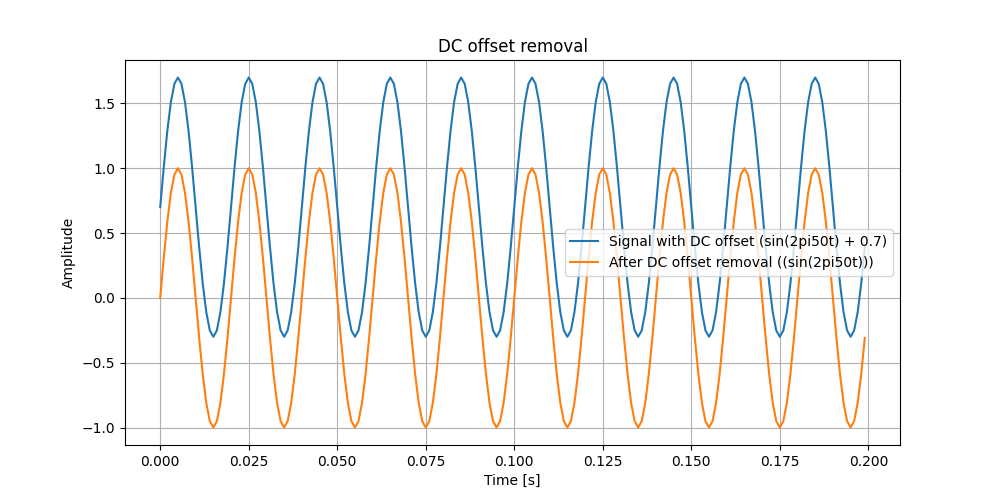
\includegraphics[width=0.7\linewidth]{Figures/dc offset removal.png}
    \caption[  DC offset comparison]{Comparison of the signal with a DC offset of 0.7, and the signal with the DC offset removed.}
    \label{fig:DC_offset}
    \end{figure}
    \newpage
    \subsubsection{WAV file generation}
    The measured and offset signal before the further analysis, has to be converted to a \textbf{.wav} type file. The main reason for that was the use of the sound file in the debuging and testing process, and the possibility to use some of the member functions present in the \textbf{librosa} library, which was extencively used in the feature extraction process. The code responsible for the conversion of the signal can be seen in Code~\ref{lst:wav_file}.

\begin{lstlisting}[style=pythonstyle, caption={Class for the conversion of the signal to the wav file.}, label={lst:wav_file}]
from scipy.io.wavfile import write
from receivers.stm32_usb_receiver import STM32UsbReceiver
import numpy as np

class WavCreation:
    """
    Creates the wav sound file, using samples gathered with 
    stm32_usb_receiver
    
    Has one func called convert_into_wav(), that write the sound file into recordings folder. 
    """
    def __init__(self):
        pass

    def convert_into_wav(self, samples : np.ndarray, receive_time : STM32UsbReceiver, duration : STM32UsbReceiver):
        filename =f"debug_figures/04_05_drone_test_riktig_plassering/mic_recording{receive_time}.wav"
        effective_fs = len(samples[0])/ duration
        #print([len(ch) for ch in samples])
        #print(samples.shape)
        #print(samples.dtype)
        #print(effective_fs)
        audio = np.stack(samples, axis=1)
        audio = np.clip(audio, -32768, 32767).astype(np.int16)
        write(filename,int(round(effective_fs)), audio)

\end{lstlisting}  

\newpage
\subsection{Feature Extraction}
    The feature extruction is conducted by calling the \textbf{extract\_features()} which is an external method of the feature extraction class that can be accesed in \textbf{Drone\_detection\_porgram\_bachelor/features/mfcc\_extraction.py}. The class was initialized with the parameters shown in Table~\ref{tab:mfcc_parameters}. The feature extraction method is mainly based on the ideas taken from (\cite{singh2014mfcc} and \cite{zheng2001mfcc}).

    \begin{table}[h]
\centering
\caption{Parameters used in the MFCCExtractor class}
\label{tab:mfcc_parameters}
\begin{tabular}{|c|c|c|}
\hline
\textbf{Parameter} & \textbf{Value} & \textbf{Description} \\
\hline
\texttt{n\_mfcc} & 40 & Number of MFCC coefficients \\
\hline
\texttt{n\_fft} & 1024 & FFT size used for spectral analysis \\
\hline
\texttt{hop\_length} & 250 & Number of samples between consecutive frames \\
\hline
\texttt{win\_length} & 500 & Window length used for each frame \\
\hline
\texttt{n\_mels} & 40 & Number of Mel filters \\
\hline
\end{tabular}
\end{table}
    
    The \textbf{extract\_features()} returns the accumulated features representing the spectral behaviour of the signal, and can be seen in Code~\ref{lst:extract:features}. The function is based on the internal methods, that were used to simplify the process of extracting the spectral features of the measured signal.

    \begin{lstlisting}[style=pythonstyle, caption={Definition of the extract\_features method.}, label={lst:extract:features}]
    def extract_features(self, audio_file):
        self._convert_wav_to_signal(audio_file)
        self._mfcc_after_preemphasis()
        self._create_mel_spec()
        self._power_mel_spec()
        self._accumulate_the_stats()
        return self.acc_features
    
    \end{lstlisting}
    \newpage
    \subsubsection{Extraction pipeline}
    The feature extraction pipeline, can be seen in Figure~\ref{fig:mfcc_pipeline}, which describes how the features are extructed and then exported. 
    
    \begin{figure}[h]
        \centering
        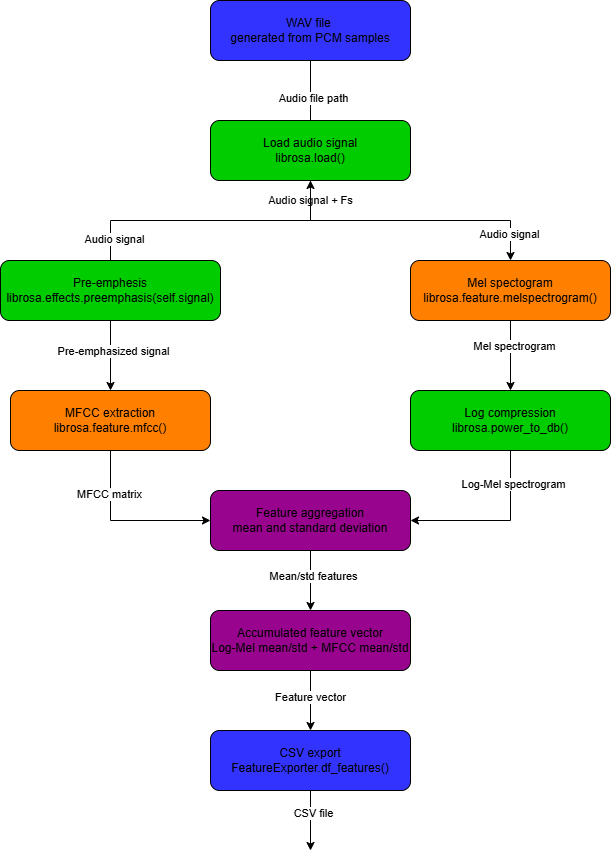
\includegraphics[width=0.48\linewidth]{Figures/mfcc_pipeline.png}
        \caption[  Flowchart- feature extraction]{Feature extraction pipeline}
        \label{fig:mfcc_pipeline}
    \end{figure}
    
    \subsubsection{Wav conversion}
    The first stage of the feature extraction process is conducted in the\\
    \textbf{\_convert\_wav\_to\_signal()}, which uses the \textbf{.load()} function from the Librosa library. The .load() function, process the wav file and converts it into an array representing the signal, and also returns a scalar representing the signals FS. The functions declaration can be seen in Code~\ref{lst:wav_to_signal}.

    \begin{lstlisting}[style=pythonstyle, caption={The function used to convert the wav file into an array of samples}, label={lst:wav_to_signal}]
    def _convert_wav_to_signal(self, audio_file):
        self.signal, self.fs = librosa.load(audio_file, sr = None)
        self.signal_time_domain = self.signal
    \end{lstlisting}
    
    \subsubsection{Pre-emphesis}
        The pre-emphesis was conducted by applying a method from the librosa library, which is based on the following filter design Equation~\ref{eq:n-order_diff_filter}], which represents the first-order differencing filter (\cite{librosaPreemphasis}). The pre-emphesis was applied to amplify the high frequency components present in the signal, by using the default settings in the Librosa method, such as coef being equal 0.97.

    \begin{equation}
        \label{eq:n-order_diff_filter}
        y[n] -> y[n] - coef*y[n-1]
    \end{equation}

    \subsubsection{MFCC extraction}
    \raggedbottom
    In the project the MFCC are used to describe the overall spectral shape of the measured acoustic signal.
    The extraction of the mfcc is conducted in \textbf{\_mfcc\_after\_preemphesis()} seen in Code~\ref{lst:mfcc_function}, which takes the pre-emphasised signal and the sampling frequency, and uses them as the base of the feature extraction. The extraction itself is conducted by applying the \textbf{feature.mfcc()} method taken from librosa, which uses the values initializing the class object as in the Table~\ref{tab:mfcc_parameters}.\\
    \begin{lstlisting}[style=pythonstyle, caption={Function used for the mfcc extraction}, label={lst:mfcc_function}]
    def _mfcc_after_preemphasis(self):
        signal_preemphasised = self._get_preemphasised_signal()

        self.mfcc = librosa.feature.mfcc(
            y = signal_preemphasised,
            sr = self.fs,
            n_mfcc= self.n_mfcc,
            n_fft = self.n_fft,
            hop_length = self.hop_length,
            win_length = self.win_length,
            n_mels = self.n_mels
        )
    \end{lstlisting}
    Beside the pre-emphasized signal and its sampling frequency, the method uses the following arguments:\\
    \begin{enumerate}
        \item \textbf{n\_mfcc} - represents the number of coefficients used to describe the spectrum present in each frame. The higher number of coefficients allows for a wider representation of the spectrum, but at the same time increases the computational time needed to extract the spectral information, represented by each coefficient. The value used in the project is 40, which gave accurate enough representation of the spectrum, without much of a time delay.\\
    \item \textbf{n\_fft} - represents the number of points used for the frequency analysis of the signal. The higher the value the lower the spacing between the frequency bins, allowing for more accurate representation of the energy division between the frequency components. The value used in the project is 1024, which in combination with the Fs of around 20 Khz, gives around 19.5 Hz per frequency bin.\\
    \item \textbf{hop\_length} - defines the sample distance between the consecutive frames. In this project, the length of 250 samples was used, which divided by the Fs of 20 Khz, gives around 12.5 ms between each frame. The reason for the use of that particular number, was the assumption of 50\% overlap between the frames, where each frame is expected to hold 500 samples.\\
    \item \textbf{win\_length} - represents the number of samples present in each frame, where each frame has to represent around 25 ms. To find the number of samples needed to represent the time period of 0.025 seconds, the desired period has to be multiplied by Fs of 20 Khz which gives 500 samples.
    \item  \textbf{n\_mels} - represents the number of Mel-scaled band-pass filters, which are applied to the signal to convert it into Mel frequency spectrum. The number of the filters used is 40, which is two times the number of filters used in (\cite{singh2014mfcc}), to increase the details of the signal. 
    \end{enumerate}

    After the extraction the MFCC are saved in the extraction object. 
    
    \subsubsection{Log-Mel spectrogram}
    In the project, the log-mel spectrograms are used to describe the energy distribution across the Mel-frequency bands over time. 
    The Mel spectrogram is generated using the \textbf{librosa.feature.melspectrogram()} method, which uses the same frame-based parameters as the MFCC extraction method. To obtain the  logharitmic representation of the spectral energy, the \textbf{librosa.power\_to\_db()} method is applied. The Log-Mel spectrogram was extracted because it represent the energy distribution of the signal across the Mel-frequency bands, which allows to describe where in the Mel-frequency spectrum most of the signal energy is located.
    
    \subsubsection{Feature aggregation}
    The features from the MFCC and Log-mel spectrogram are being accumulated to create a fixed-size feature vector for each recorded signal. This is necessary because both methods return values based on the analysis frame, where each frame contains a set of MFCC coeffieicents or Mel-frequency band energies. The total number of frames will change, if the recording is shortened due to any microphone mulfunction present, which could introducce a situation where one recording is represented by fewer frames then the previous one. This could make the signal incompatible with the classifier, as it expects a fixed-size feature vectors. Hence the features are aggregated by taking a mean and standard deviation (std) of the Log-Mel and MFCC coefficients. The mean value of the Log-Mel represents the average energy distribution, while the mean of the MFCC represents the average spectral shape. The std of the MFCC shows how the whole spectrum changes over time, while the std of the Log-Mel, represents how much enregy in each band changes over time. The funtion responsible for the aggregation is called \textbf{\_accumulate\_the\_stats} and can be seen in Code~\ref{lst:accumulate_the_stats}.
    
    \begin{lstlisting}[style=pythonstyle, caption={Function used for feature accumulation}, label={lst:accumulate_the_stats}]
    def _accumulate_the_stats(self):
        # mffcc mean - avg spectral shape, or how the sound looks like in the spectrum. Is it more "flat" or "steep" or "curved"
        # mfcc std - how much the whole spectral envelope changes over time 

        # log-mel mean - how the energy is distirbuated across freq bands (in db)
        # low-mel std - how much energy in each band changes over time

        logmel_stats = np.hstack([self.log_mel_spec.mean(axis=1), self.log_mel_spec.std(axis=1)])
        mfcc_stats = np.hstack([self.mfcc.mean(axis=1),self.mfcc.std(axis=1)])
        self.acc_features = np.hstack([logmel_stats,mfcc_stats])
    \end{lstlisting}

    
\subsection{Direction of arrival estimation (DOA)}
The direction of arrival estimation of the detected drone was conducted by using the\\ \textbf{gcc\_processor.py} and \textbf{doa\_estimator.py} modules. The flow chart for the TDOA estimation pipeline can be seen in Figure~\ref{fig:doa_estimation}. The method is mainly a mix of ideas taken from (\cite{kwon2010gccphat}, \cite{kang2016prefiltering} and \cite{blandin2012multisource}). 

\begin{figure}[h]
    \centering
    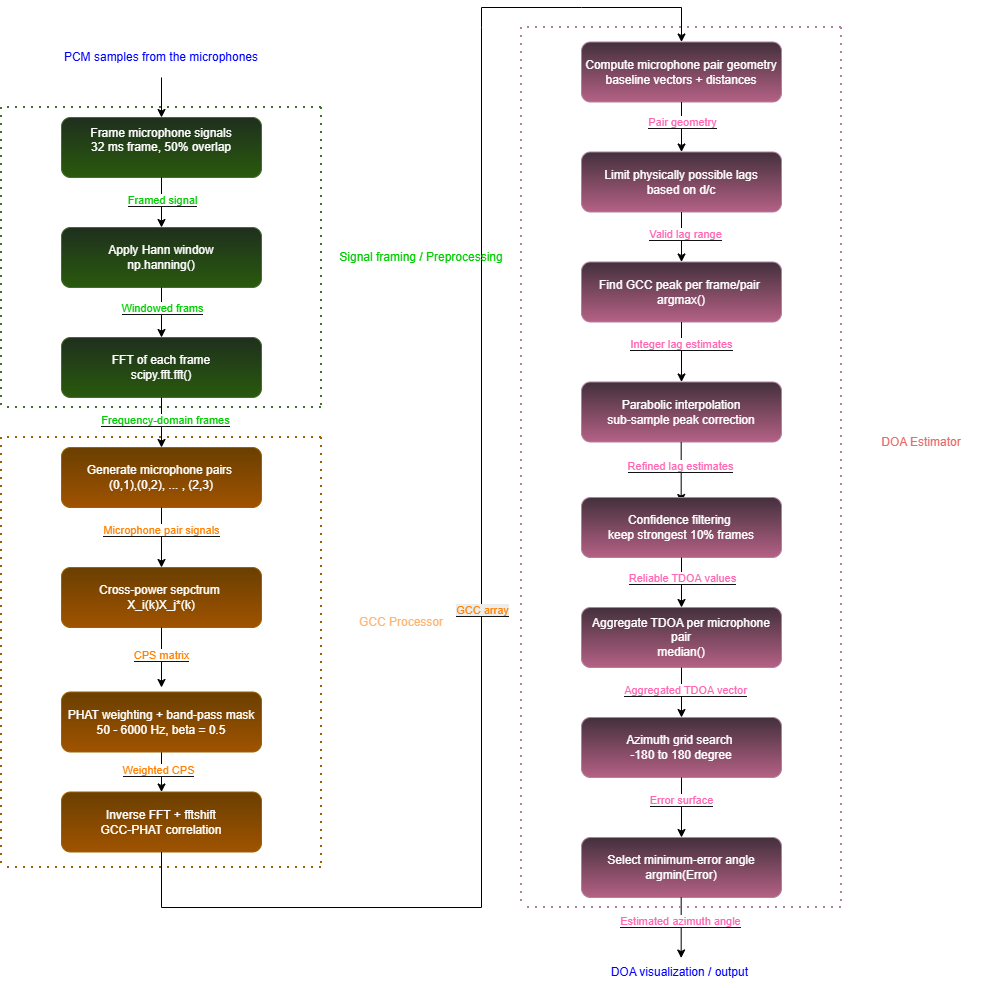
\includegraphics[width=0.6\linewidth]{Figures/gcc_flow_chart.drawio (5).png}
    \caption{DOA estimation pipeline}
    \label{fig:doa_estimation}
\end{figure}


    \subsubsection{GCC processor}
    The gcc\_processor module processes the microphone signals in pairs by framing the signals, applying a window function, calculating the FFT, and computing the cross-power spectrum between each microphone pair. The CPS is then weighted using the PHAT method, and transformed back to the time doamin the GCC-PHAT correlation function (\cite{kwon2010gccphat}). To produce the weighted CPS values, the \textbf{process\_signal} function as seen in Code\ref{lst:process_signal}, has to called with the measured signal as an argument.\\

    \begin{lstlisting}[style=pythonstyle, caption={Function used to produce the correlation matrix of the microphone.}, label={lst:process_signal}]
    def process_signal(self, samples: np.ndarray, fs): #samples has to be np.array to use .shape
        self.fs = fs
        samples_per_frame = int(self.fs * self.frame_ms / 1000)
        frames = self._frame_samples(samples, samples_per_frame)
        windowed_frames = self._window_each_frame(frames)
        frames_fft = self._fft_each_frame(windowed_frames)
        cps_array = self._cross_power_spectrum(frames_fft)
        gcc_array = self._p_hat_weighted_gcc(cps_array, fs, samples_per_frame)
        return gcc_array
    \end{lstlisting}    
    
    \paragraph{Signal framing}
    The signal framing is done in the \textbf{\_frame\_samples} method, which can be seen in Code~\ref{lst:frame_sample_gcc}. The reason for the framing application is the same as for the framing of the signal for the MFCC, namely the need of representing the signal as stationary for the application of FFT. \\

    \begin{lstlisting}[style=pythonstyle, caption={Function used for signal framing for gcc.}, label={lst:frame_sample_gcc}]
    def _frame_samples(self,samples: np.ndarray, samples_per_frame):
        if samples is not None:
            frames = []
            samples_n = samples.shape[1]
            hop = samples_per_frame//2
            for frame_n in range(int(samples_n/hop)):
                start = frame_n * hop
                end = start + samples_per_frame

                if end <= samples_n:
                    frames.append(samples[:, start:end])
            return np.array(frames)
        else:
            raise RuntimeError("No samples present, gather them again")
    \end{lstlisting}
    \newpage
    \paragraph{Windowing}
    The windwing is conducted to reduce the effects of the spectral leakage. The function \textbf{\_window\_each\_frame()} does so by using the \textbf{hanning} from the numpy library, which multiplies the signal by the hann window function, resulting in a signal with reduced spectral leakage. The function was applied as seen in Code~\ref{lst:window_gcc}.\\

    \begin{lstlisting}[style=pythonstyle, caption={Function used for windowing the signal.}, label={lst:window_gcc}]
    def _window_each_frame(self,frames: np.ndarray):
        hanning = np.hanning(int(frames.shape[-1]))
        windowed_frames = frames * hanning
        return windowed_frames
    \end{lstlisting}
    
    \paragraph{FFT and cross-power spectrum}
    The CPS is found by calling the \textbf{\_cross\_power\_spectrum()} function, which expects to receive the frames in the frequency-domain. The transformation of the time-domain frames into the frequency domain is conducted by using the \textbf{\_fft\_each\_frame()} method. The FFT of one microphone signal is later multipplied by the complex conjugate of the FFT of the other microphone signal as introduced in the theory section. The microphone pairs were generated by using the \textbf{\_generate\_mic\_pairs()}, which returns all unique microphone pair combinations. For four microphones, this results in six microphone pairs. The methods used for the FFT, pair generation and the CPS calculations are shown in Code~\ref{lst:fft_and_cps}.\\

    \begin{lstlisting}[style=pythonstyle, caption={Functions used to fing the CPS of the microphone pair, before the PHAT weighting.}, label={lst:fft_and_cps}]
    def _fft_each_frame(self,frames):
        frames_frq_domain = fft(frames, axis=-1)
        return frames_frq_domain
    
    def generate_mic_pairs(self, n_mics): # is quite needed in the tdoa and doa
        return [(i,j) for i in range(n_mics) for j in range(i+1, n_mics)]

    def _cross_power_spectrum(self,frames_fft:np.ndarray):
        # try to vectorize?
        # use list comprahension?
        cps = []
        n_frames = frames_fft.shape[0]
        n_mics = frames_fft.shape[1]
        self.n_mics = n_mics

        if self.mic_pairs is None:
            self.mic_pairs = self.generate_mic_pairs(n_mics)
        
        mic_pairs = self.mic_pairs

        # for each frame multi mic_i with the conjugate of mic_j

        for frame in range(n_frames): 
            frame_cps = [] # cps of one frame
            for i,j in mic_pairs:
                cps_ij = frames_fft[frame, i, :] *frames_fft[frame,j,:].conj()
                frame_cps.append(cps_ij)
            cps.append(frame_cps)

        # frame_cps shape (frame, mic pair, cps)
        return np.array(cps)
        \end{lstlisting}
    
    \paragraph{PHAT weighting}
    After the CPS between the microphones was estimated, the PHAT weighting has to be applied to reduce the influence of high-amplitude frequency components, which is accomplished by calling the\\
    \textbf{\_p\_hat\_weighted\_gcc()} function. Inside of the method, the CPS values are divided by CPS magnitude raised to the power of $\beta$, as introduced in the theory part based on (\cite{kang2016prefiltering}). To the magnitude of the CPS, the epsilon of 1e-13 was also added, to avoid the division by zero. The scaling value of $\beta$ used in the project is 0.5, which was chosen to be an initial testing value, before the application of the SNR based $\beta$ value estimation. After the weighting was conducted, the CPS values are also filtered by a frequency mask of frequency interval of 80 Hz to 6000 Hz. The frequency for the frequency mask was chosen long before the testing on the live drone was conducted. The weighted CPS values are then transformed back to the time-domain, where they represent the correlation between the microphones over the possible time lags. The result is then shiftet to be centered around zero. The declaration of function used can be seen in Code~\ref{lst:phat_weighting}.\\

    \begin{lstlisting}[style=pythonstyle, caption={Function used to weight the CPS values.}, label={lst:phat_weighting}]
    def _p_hat_weighted_gcc(self,cps_array :np.ndarray, fs, n_samples_per_frame, freq_low = 80, freq_high = 6000, beta = 0.5, eps = 1e-13, use_adaptive_beta = False ):
        freq = np.fft.fftfreq(n_samples_per_frame, d = 1/fs) # array of freq for each fft bin
        band = (freq_low <= np.abs(freq)) & (np.abs(freq) <= freq_high) # boolean mask to remove unwanted freq
        mag = np.abs(cps_array) + eps
        
        weighted_cps = cps_array/(mag**beta)
        weighted_cps *= band 
        gcc_array = np.fft.ifft(weighted_cps, axis =-1)
        gcc_array = np.fft.fftshift(gcc_array, axes = -1)

        return np.real(gcc_array)
    \end{lstlisting}


        
    \subsubsection{DOA estimator}
    The doa\_estimator uses resulting time-delay information from the microphone pairs and compares it with simulated TDOA values for different azimuth angles. The azimuth angle with the best match is then selected as the estimated DOA of the sound source. The code responsible for the DOA estimation, can be seen in Code~\ref{lst:doa_estimation}.

    \begin{lstlisting}[style=pythonstyle, caption={Function used to estimate the DOA}, label={lst:doa_estimation}]
     def estimate_DOA(self):
        self._compute_pair_geometry()
        self._compute_lags_per_pair()
        self._estimate_tdoa()
        self._estimate_azimuth()
    \end{lstlisting}
    \newpage
    \paragraph{Pair geometry}
    For the system to properly estimate direction of the sound source, the baseline vector and the norm of each microphone pair has to be computed.
    The baseline vector describes the relative position between the two microphones and is found by subtracting one microphone position from the other. The norm gives the physical distance between the microphones, which is later used to calculate the maximum possible time delay for each pair. The baseline vectors and norms are computed by calling \textbf{\_compute\_pair\_geometry()}, as shown in Code~\ref{lst:pair_geometry}.\\  

    \begin{lstlisting}[style=pythonstyle, caption={Function used to compute the pair geometry.}, label={lst:pair_geometry}]
    def _compute_pair_geometry(self):
        # Finds the baseline vectors, normalize them and creates the baseline unit vectors
        if self.gcc_processor.mic_pairs is None:
            raise RuntimeError("No microphone pairs found, and probably the cross power spectrum is also absent. Run gcc_processor.process_signal in main.py")

        mic_pairs = self.gcc_processor.mic_pairs
        
        self.baseline_vecs = []
        self.baseline_vec_norms = []
        
        for i,j in mic_pairs:
            baseline_vec_ij = self.p_vector[:, i] - self.p_vector[:,j]
            self.baseline_vecs.append(baseline_vec_ij)
            baseline_vec_norm = np.linalg.norm(baseline_vec_ij)
            self.baseline_vec_norms.append(baseline_vec_norm)
    \end{lstlisting}

    \paragraph{Lag constraints}
    Since a sound wave is unable to travel faster then the speed of sound, the maximum possible TDOA for each microphone pair can be computed by dividing the distance, between the microphones by the speed of sound. This maximum time delay is then converted into a maximum lag in samples using the sampling frequency. The resulting value, can then be used to define the maximum and minimum physically possible lag around the centered zero lag. The lag constraints are computed by calling the \textbf{\_compute\_lags\_per\_pair}, which can be seen in Code~\ref{lst:compute_pair_lags}.\\

    \begin{lstlisting}[style=pythonstyle, caption={Function used to compute the pair lags.}, label={lst:compute_pair_lags}]
    def _compute_lags_per_pair(self):
        t_delay_max_arr = [baseline_norm/self.speed_of_sound for baseline_norm in self.baseline_vec_norms]
        max_lag_samples = [int(np.ceil((t_delay_max_pair) * self.gcc_processor.fs)) for t_delay_max_pair in t_delay_max_arr] 
        
        if self.gcc_array is None:
            raise RuntimeError("GCC array is empty, run set_gcc_array in main.py.")
        
        self.n_frames = self.gcc_array.shape[0]
        k_bins = self.gcc_array.shape[2]
        self.lag_center = k_bins // 2

        self.lag_min= [max(0,self.lag_center - max_lag_samples_pair) for max_lag_samples_pair in max_lag_samples]
        self.lag_max = [min(k_bins, self.lag_center + max_lag_samples_pair + 1) for max_lag_samples_pair in max_lag_samples]
    \end{lstlisting}
    \newpage

    \paragraph{Estimated TDOA}
    The TDOA between each microphone pair, is estimated using the GCC array explained in the previous section, where the delay is found from the peak of the GCC function (\cite{kwon2010gccphat}). The GCC values are sliced into segemtns based on the pair used in the current iteration, and the maximum an minimum lag possible for the microphone pair. The peaks for each segment are later found and interpolated using the \textbf{\_delta\_newton\_approx}, to make the derived top, to be closer to the actual maxima.
    As the signal is expected to hold some noise, to reduce the influence of it, a confidence value is calculated for each frame. The confidence value is a ratio between the peak values found during the iteration, and the median of the segment values. By using the median, the result is expected to be less exposed to the influence of the outlier samples. The frames are later reduced in number to 10\% of frames with the highest confidence value, to additionaly reduce the influence of the noise. The time delays of these selected frames are than accumulated by taking the median value, which gives the final TDOA estimation for each microphone pair. 
    
    \begin{lstlisting}[style=pythonstyle, caption={Function used to estimate the TDOA between the microphones.}, label={lst:estimated_tdoa}]
     def _estimate_tdoa(self): 
        if self.gcc_array is None:
            # gcc_array.shape = ( frames, pairs,  bins)
            raise RuntimeError("GCC array is empty, run set_gcc_array.")
        if self.lag_center is None:
            raise RuntimeError("The lag center is non existant, run _compute_lags_per_pair.")
    
        self.aggregated_time_delay_list = []
        keep_frac = 0.1 # used 0.1 before
        fs = self.gcc_processor.fs

        for pair_indx in range(self.gcc_array.shape[1]):
            lag_min = self.lag_min[pair_indx]
            lag_max = self.lag_max[pair_indx]

            segment = self.gcc_array[:, pair_indx, :][:, lag_min:lag_max]
            peaks = np.argmax(segment, axis=1)
            
            deltas = np.array([
                self._parabolic_interpolation(segment[n], peaks[n])
                for n in range(self.n_frames)
            ])
            lag_samples = (lag_min + (peaks + deltas)) - self.lag_center
            peak_vals = segment[np.arange(self.n_frames), peaks]
            ## CHAT GPT ###
            #mean_vals = np.mean(segment, axis = 1)
            median_values = np.median(segment, axis=1)
            #confidence = peak_vals/(mean_vals + 1e-15)
            confidence = peak_vals/(median_values + 1e-15)
            time_delays = lag_samples/fs 
            k = max(1, int(np.ceil(keep_frac * self.n_frames))) # keeps x% of frames
            indx = np.argsort(confidence)[-k:] # sorts all of the frames from lowest to the highest confidency score, and keeps the last k elements, which are the highest 
            aggregated_time_delay = np.median(time_delays[indx])
            self.aggregated_time_delay_list.append(aggregated_time_delay)
            
            ### ### ### 
        self.aggregated_time_delay_list = np.array(self.aggregated_time_delay_list)

    \end{lstlisting}
    \newpage
    \paragraph{Sub-sample interpolation}
    Since the peaks in the segment were found at discrete samples, it is possible that peak represented by the lag might not be the true physcial peak (\cite{lai1999interpolation}). Hence the \textbf{\_parabolic\_interpolation()} function was implemented based on the three point parabolic interpolation method that can be seen in Code~\ref{lst:parabolic_interpolation}. The method assumes that the peak and the nearby values may be represented as a parabola as shown in Equation~\ref{eq:parabola} from (\cite{lai1999interpolation}).

    \begin{equation}
    \label{eq:parabola}
    y(x) = ax^2 + bx + c
    \end{equation}

    According to \cite{lai1999interpolation}, the location of the maximum coefficient $\delta$ can be estimated as in Equation~\ref{eq:max_parabola}.

    \begin{equation}
        \label{eq:max_parabola}
        \delta = -\frac{b}{2a}
    \end{equation}

    Which by using the peak value and its two neighbouring values can be estimates as in Equation~\ref{eq:interpolation_using_neighbours} taken from \cite{lai1999interpolation}.

    \begin{equation}
        \label{eq:interpolation_using_neighbours}
        \delta =\frac{y(-1)-y(1)}{2\left(y(-1)-2y(0)+y(1)\right)}
    \end{equation}

     The resulting $\delta$ is then added to the detected integer peak position before the lag is converted into a time delay. 
     
    
    \begin{lstlisting}[style=pythonstyle, caption={Function used for interpolation, based on \cite{lai1999interpolation}.}, label={lst:parabolic_interpolation}]

    def _parabolic_interpolation(self,y,k):
        if k <= 0 or k >= len(y) - 1:
            return 0

        y_minus = y[k - 1]  # y(-1)
        y_zero = y[k]       # y(0)
        y_plus = y[k + 1]   # y(1)

        denominator = 2 * (y_minus - 2 * y_zero + y_plus)

        if np.abs(denominator) < 1e-15:
            return 0.0
    
        delta = (y_minus - y_plus) / denominator
        return float(delta)

    \end{lstlisting}
    \newpage
    \paragraph{Azimuth estimation}

    The azimuth estimation is conducted by simulating TDOA values for different candidate angles around the tower, as shown in Code~\ref{lst:estimated_azimuth}. The angles are generated from \(-180^\circ\) to \(180^\circ\), with a resolution of \(0.1^\circ\). For each of these angles, the expected TDOA values are calculated and compared with the measured TDOA values. The angle which gives the lowest total error is then selected as the estimated azimuth.

    The implementation is based on the TDOA based source localization method described in Chapter 8.3.3 in \cite{brandstein2001microphonearrays}. In this method, the theoretical TDOA for a microphone pair is found from the difference in distance between a hypothetical source position and the two microphones in the pair, divided by the speed of sound. In this project, the hypothetical source position is limited to the horizontal plane, since only the azimuth angle is estimated. This also fits the microphone setup, where the microphones are placed in the same \(z\)-axis plane.

    For each candidate angle \(\phi\), a hypothetical source position \(q(\phi)\) is generated as shown in Equation~\ref{eq:hyp_source_position}. The value \(R\) represents the radius from the tower. Since the system estimates only the direction and not the distance to the source, this radius is set to an arbitrary value of 1. The \(x\)- and \(y\)-coordinates are represented by \(\cos(\phi)\) and \(\sin(\phi)\), while the \(z\)-coordinate is set to zero because the elevation is not estimated.

    \begin{equation}
        q(\phi) = R
        \begin{bmatrix}
            \cos(\phi) \\
            \sin(\phi) \\
            0
        \end{bmatrix}
        \label{eq:hyp_source_position}
    \end{equation}

    For each microphone pair in the system, the predicted TDOA is calculated using the difference in distance between the microphones in the pair, divided by the speed of sound, as shown in Equation~\ref{eq:predicted_tdoa}, which is  based on the Equation~8.10 from \cite{brandstein2001microphonearrays}.

    \begin{equation}
        \tau_{ij}^{pred}(\phi) =
        \frac{\left\|q(\phi)-p_i\right\|-\left\|q(\phi)-p_j\right\|}{c}
        \label{eq:predicted_tdoa}
    \end{equation}

    For each microphone pair, the predicted TDOA is subtracted from the measured TDOA and square which describe the error between the values. The squared error is then summed for each microphone pair, giving one total error value for the current candidate angle as seen in \ref{eq:azimuth_error} taken from Equation~8.12 \cite{brandstein2001microphonearrays}. This follows the same principle as the example equation, but in this implementation the sound source position is restricted to the generated azimuth values.

    \begin{equation}
        E(\phi) =
        \sum_{(i,j)}
        \left(\tau_{ij}^{meas} - \tau_{ij}^{pred}(\phi)\right)^2
        \label{eq:azimuth_error}
    \end{equation}

    The final azimuth estimate is the candidate angle that minimizes the total error, as shown in Equation~\ref{eq:azimuth_argmin}, which is based on Equation~8.13 from \cite{brandstein2001microphonearrays}.

    \begin{equation}
        \hat{\phi} = \arg\min_{\phi} E(\phi)
        \label{eq:azimuth_argmin}
    \end{equation}
    
    
    \newpage
    \begin{lstlisting}[style=pythonstyle, caption={Function used to estimate the azimuth of the sound source.}, label={lst:estimated_azimuth}]
     def _estimate_azimuth(self): # only finds the azimuth of the target, not the elevation
        if self.aggregated_time_delay_list is None:
            raise RuntimeError("Time delyas are empty, Run _estimate_frame_lags_for_pair first")

        azimuth_grid_deg = np.linspace(-180, 180, 3601) # 3601 give 0.1 resolution, otherwise use 360 to get 1 degree res
        azimuth_grid_rad = np.radians(azimuth_grid_deg)

        R_test = 1 # arbitrary radius (far -field approxiation)
        error_surface = []
        mic_pairs = self.gcc_processor.mic_pairs

        for phi in azimuth_grid_rad:
        # hyphotesized source position q 
            u = np.array([np.cos(phi), np.sin(phi),0])
            q = R_test * u
            pair_errors = []

            for pair_indx, (i,j) in enumerate(mic_pairs):
            # eq: 8.10
                predicted_tdoa = (np.linalg.norm(q - self.p_vector[:, i]) - np.linalg.norm(q - self.p_vector[:, j]))/self.speed_of_sound

            #eq: 8.12 
                error = (self.aggregated_time_delay_list[pair_indx] - predicted_tdoa)**2
                pair_errors.append(error)

            error_surface.append(np.sum(pair_errors))
        error_surface = np.array(error_surface)

        best_indx = np.argmin(error_surface)
        self.estimated_azimuth_rad = azimuth_grid_rad[best_indx]
        self.estimated_azimuth_deg = azimuth_grid_deg[best_indx]
    \end{lstlisting}
    % and add the grid search 
\newpage
\subsection{Visualization and debugging}
For the debugging purposes, the project follows with visualization modules that can allow the user to investigate the signals beahviour during different stages of the signal analysis. 

    \subsubsection{USB receiver debug}
    To visualize and export the signal sent by the STM32, the program uses the \textbf{stm32\_usb\_receiver\_debug\_tool.py} module, which can create a figure containg four plots, each representing a time domain signal, and additionaly creates a dataframe object containing the raw signal data.
    
    \subsubsection{DOA visualizer}
    DOA visualizer, was developed to visualize the estimated direction of arrival of the detected sound source in relation to the systems position. The module, creates a figure with two circles. The circle centered in the middle of the figure represents the systems position, and the outer circle shows the detection area of the system. The estimated sound source is marked by a line, and a dot at the end of it.  
    
    \subsubsection{Feature visualizer}
    The feature visualizer was developed to show the energy distribution between the frequency bands present in the signal. The module allows for generation of a spectrogram and a Mel-spectogram to show the difference between the two ways of describing the signals energy distribution. The module was mainly used during the testing phase, and was ment to be used as a base for the UI system. 
 

\subsection{PCB design}
The project uses two distinct PCB designs developed by the students. The \textbf{Upper PCB} is responsible for control and supply of the stepper-motors, the compass, the Arduino nano and the upper Raspberry Pi. The \textbf{Bottom PCB} was ment to be used as the replacement for most of the functions provided by the CCA02M2, with addition of the mounting headers for the STM32 based MCU. Most of the modules were connected based on the example schematics present in the each components datasheet. The thickness and spacing of lines was decided based on the values received from the Saturn PCB Design program \cite{saturnPCBToolkit}. One such value is the thickness of the conductor, which is expected to tolarate for up to 4.5A, with the rise of the temp of 20 degrees as shown in \ref{fig:inductor_width_upper_pcb}.  
% mention the use of pcb saturn
% mention the use of fallstad for simulation
\newpage
\begin{figure}[h]
    \centering
    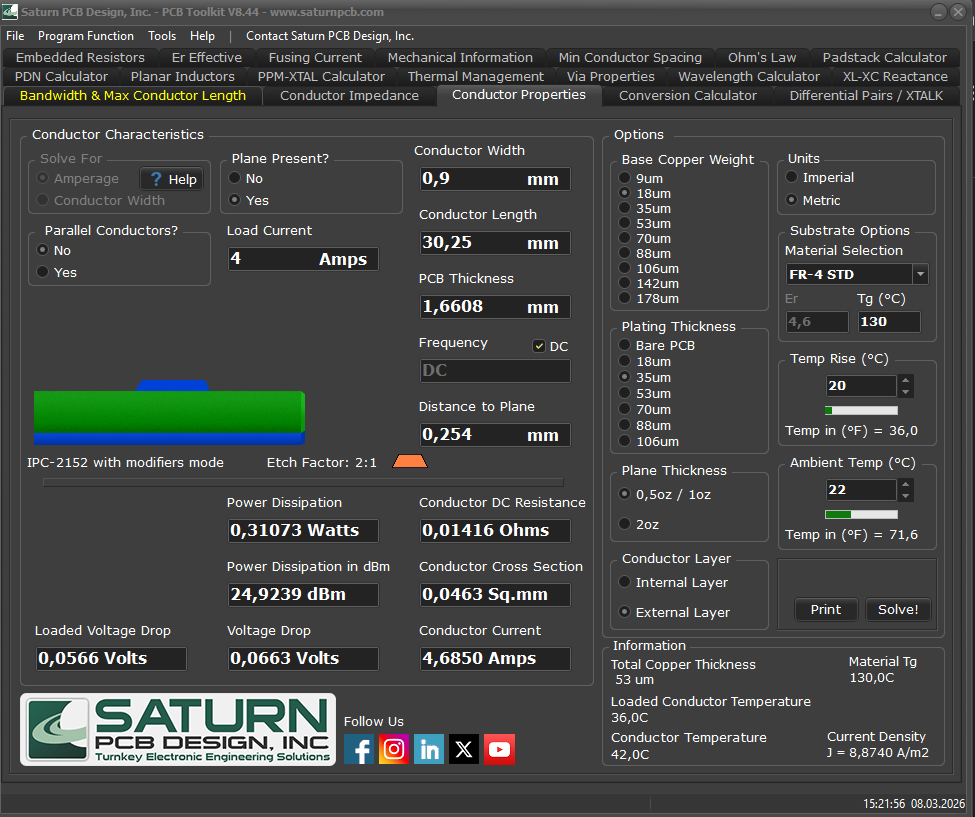
\includegraphics[width=0.5\linewidth]{Figures/inductor for upper pcb 4A.png}
    \caption[Conductor width ]{Conductor width for load of 4A for the upper PCB}
    \label{fig:inductor_width_upper_pcb}
\end{figure}

Additionally the via-points for the conductors moving through differnt planes, were also sized based on the Satrun PCB Design program, as shown in Figure~\ref{fig:via_points}. 

\begin{figure}[h]
    \centering
    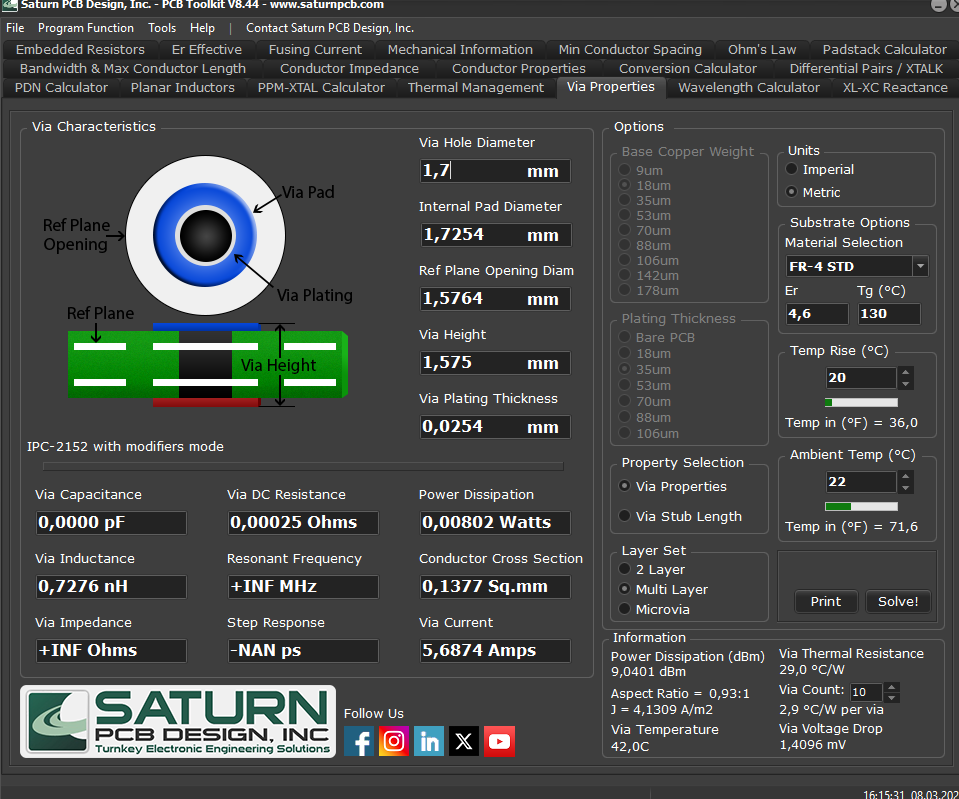
\includegraphics[width=0.5\linewidth]{Figures/via fot 5A.png}
    \caption[Via-point sizing]{Size of the via-point, that should hold for up to 5.5A}
    \label{fig:via_points}
\end{figure}

    \subsubsection{The upper PCB}
    The upper PCB is equiped in two voltage regulators of type \textbf{LM138}, where one provides the stepper-motors with 10V DC-supply, and the second provides 5V DC-supply to the Arduino nano and the Raspberry Pi. The output at the voltage regulators may be changed, by modifying the voltage ratio between the potentiometer and the restistor connected to the regulators output. The connection design was based on \cite{tiLM338}. The stepper-motors are controled by the \textbf{L6205}, which was connected according to \cite{stL6205}, where the control logic is provided by the connected Arduino nano. The compass module provided by MikroElektronika, which uses \textbf{HSCDTD008A}, was used to estimate the  relative postion of the tower. The connection diagram of the upper pcb can be seen in Figure~\ref{fig:connection_diagram_upper_pcb}, the 2D model in Figure~\ref{fig:2d_diagram_upper_pcb} and the 3D model in Figure~\ref{fig:3d_model_upper_pcb}.
    
    \begin{figure}[h]
        \centering
        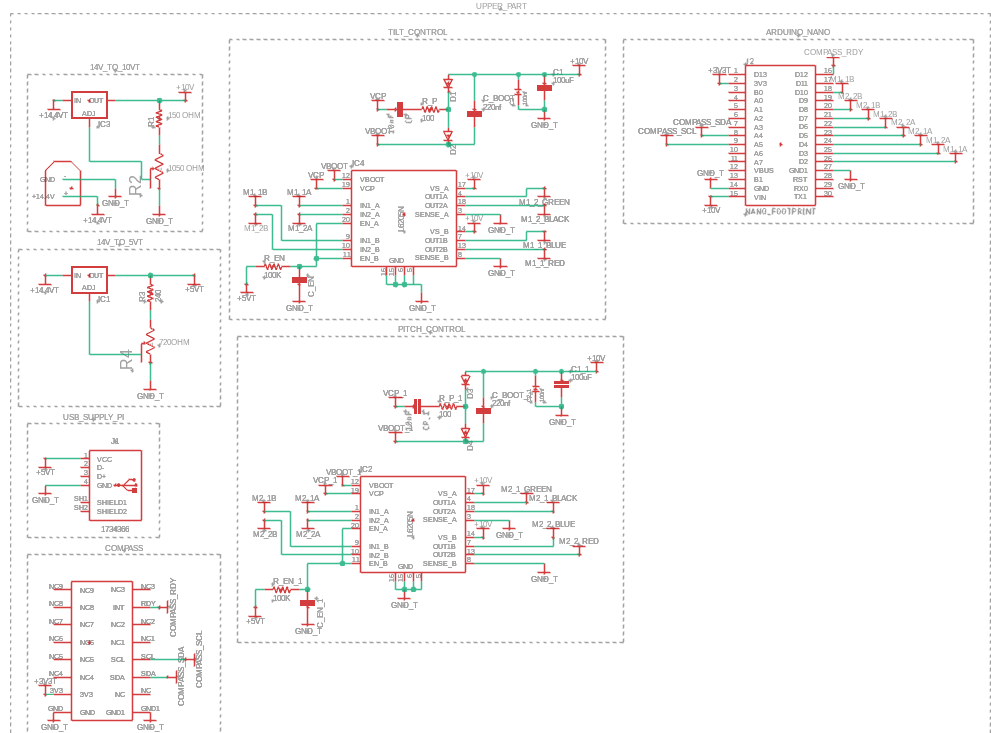
\includegraphics[width=0.75\linewidth]{Figures/upper_pcb_connection_diagram.png}
        \caption[  Connection diagram - upper PCB]{The connection diagram for the upper PCB.}
        \label{fig:connection_diagram_upper_pcb}
    \end{figure}
    \newpage
    \begin{figure}[h]
        \centering
        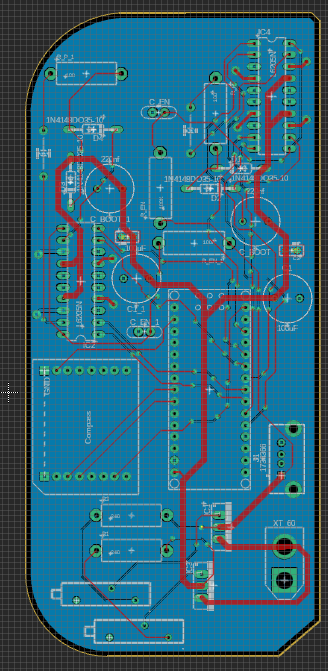
\includegraphics[width=0.25\linewidth]{upper_pcb_connections.png}
        \caption[  2D model - upper PCB]{The 2D model of the upper PCB.}
        \label{fig:2d_diagram_upper_pcb}
    \end{figure}
\newpage
    \begin{figure}[h]
        \centering
        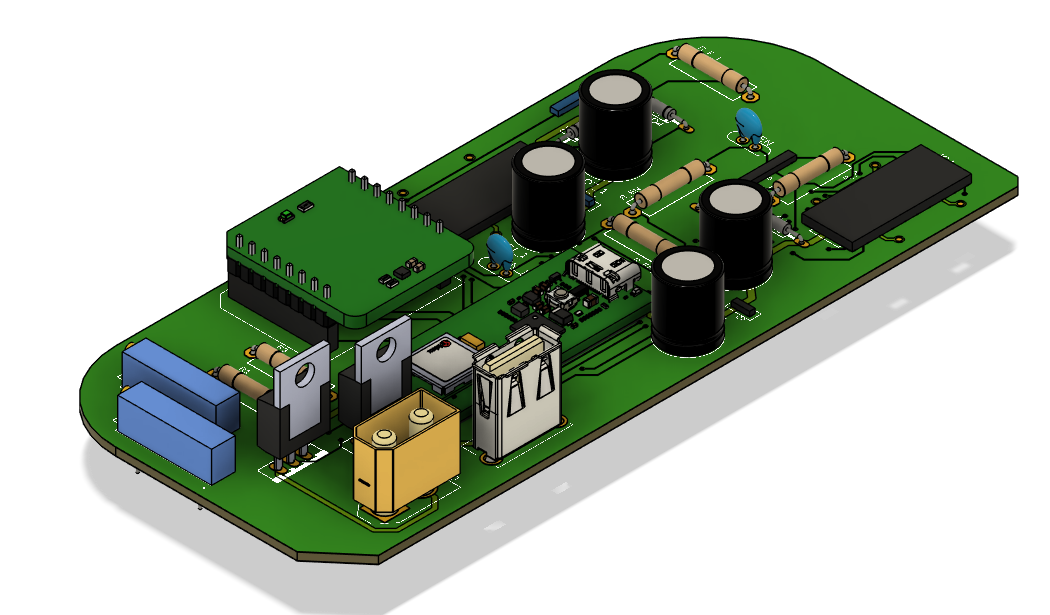
\includegraphics[width=1\linewidth]{Figures/upper_pcb_3d.png}
        \caption[  3D model - upper PCB]{The 3D model of the upper PCB}
        \label{fig:3d_model_upper_pcb}
    \end{figure}
    \newpage
    \subsubsection{Bottom PCB}
    The bottom PCB was meant to be used as the extantion board of the STM32 MCU, which was in high degree desgined based on the connection diagram of the CCA2M2 seen in \cite{x_nucleo_cca02m2_2019}. The bottom PCB just as the upper one, converts the voltage from the battery to 5V to supply the connected Raspberry Pi, and the STM32 MCU as can be seen in Figure~\ref{fig:connection_bottom_pcb}. The PCB allows for data signal from the micropohone pairs to be transferred on the same line, where one of the L/R pins of the microphones has to be put to ground, while the other to 3.3V. The Data from MCU in PCM format, is transferred to the Raspberry Pi/ PC through a microusb which is connected to an ESD unit composed of protection diodes. The 2D model of the bottom PCB can be seen in Figure~\ref{fig:2d_model_bottom_pcb}, and the 3D model in Figure~\ref{fig:3d_model_bottom_pcb},

    \begin{figure}[h]
        \centering
        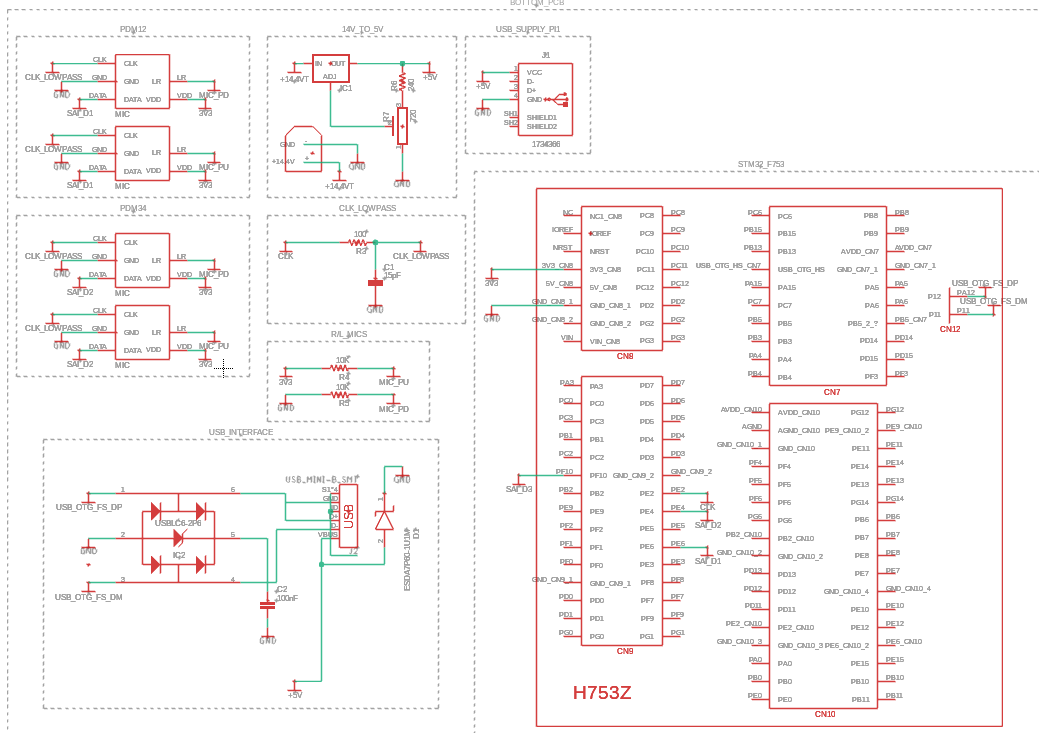
\includegraphics[width=0.75\linewidth]{Figures/connection diagram bottom pcb.png}
        \caption[  Connection diagram - bottom PCB]{The connection diagram for the bottom PCB.}
        \label{fig:connection_bottom_pcb}
    \end{figure}

    \begin{figure}[h]
        \centering
        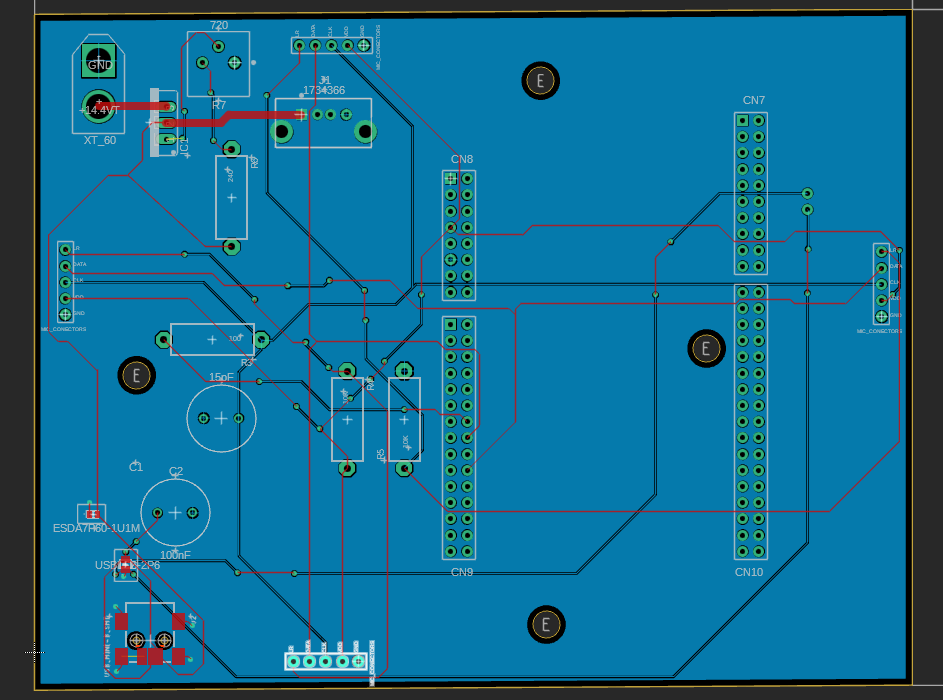
\includegraphics[width=0.5\linewidth]{Figures/2d_model_bottom_pcb.png}
        \caption[  2D model - bottom PCB]{The 2D model of the bottom PCB.}
        \label{fig:2d_model_bottom_pcb}
    \end{figure}

    \begin{figure}[h]
        \centering
        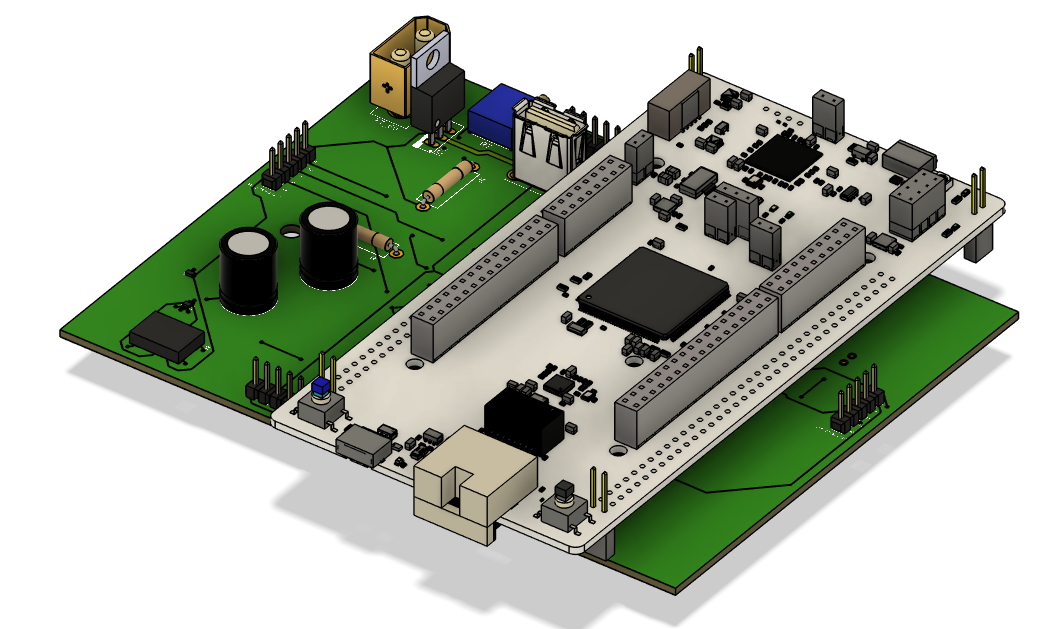
\includegraphics[width=0.85\linewidth]{Figures/3d_model_bottom_pcb.png}
        \caption[  3D model - bottom PCB]{The 3D model of the bottom PCB.}
        \label{fig:3d_model_bottom_pcb}
    \end{figure}
\newpage

\section{ML}
\subsection{YOLO implementation}

A YOLOV8n algorithm was trained on the drone dataset created by \cite{DroneDatasetFinal}. The drone dataset contains 51446 image training dataset of which there are 1 negative and 51445 positives. (\cite{DroneDatasetFinal}). The test dataset contained 5375 images of which there were 2750 negatives and 2625 positives (\cite{DroneDatasetFinal}). The classes were not balanced in the validation dataset in order to ensure that the model gets punished for false positives. mA NVIDIA RTX 4050 Laptop GPU was used during the training process with 32 GB DDR5 6400 MT/s of RAM. 

 \vspace{1em}
 
Following training, the model was exported from Ultralytics in ONNX format and converted to a Hailo Executable Format (HEF) file using the Hailo Dataflow Compiler (DFC) version 3.33.0, executed within the hailo8\_ai\_sw\_suite\_2025-10 Docker container running under WSL2. The conversion followed three sequential stages.
First, the ONNX model was parsed into a Hailo Archive (HAR) file using the hailo parser command. Because YOLOv8 uses a decoupled detection head, the six output nodes across the three detection scales were specified manually during parsing, following the node definitions provided in the Hailo Model Zoo yolov8n.yaml configuration file.
Second, the parsed HAR file was optimized using hailo optimize --hw-arch hailo8 --use-random-calib-set, which quantized the model weights from 32-bit floating point to 8-bit integer. The --use-random-calib-set flag was used in place of a representative calibration dataset, meaning quantization statistics were derived from randomly generated input data rather than real drone images.
Third, the optimized HAR was compiled to a HEF binary using hailo compiler --hw-arch hailo8. The compiler mapped the network across 8 on-chip clusters, with a total control utilization of 74.2\% and compute utilization of 43\%. Compilation completed in 9 seconds. The resulting drone\_detector.hef file was then deployed to the Raspberry Pi AI HAT+ for inference.

\subsection{YOLO testing}

In order to test the YOLO model on different drones in different settings 6 youtube videos containing drones were downloaded(tab: \ref{tab:test_videos}). The specific videos where chosen from a list of videos used by (\cite{DroneDatasetFinal}). The FLOUREON FPV racing drone video was shortened from 30 minutes to 15, due to the last 15 minutes being onboard drone footage, and therefore not useful for the qualitative test (\cite{floureon2017}). 
The YOLO model was also tested live in the lab on the flying drone, to verify that it works on the Raspberry PI. The confidence threshold used was 0.571, and it was found by anylising the F1 curve from the finished trained model. 

\begin{table}[H]
    \centering
    \caption{YouTube videos used for qualitative evaluation of the YOLOv8N drone detector.}
    \label{tab:test_videos}
    \begin{tabular}{llc}
        \toprule
        \textbf{Video} & \textbf{Drone type} & \textbf{Difficulty} \\
        \midrule
        Ryze Tello outdoor test \cite{tello2019}        & Consumer quadcopter & Easy   \\
        \$35 foldable drone review \cite{foldable2018}  & Toy quadcopter      & Easy   \\
        Karma vs Mavic vs Phantom 4 \cite{gopro2017}    & Multiple consumer   & Medium \\
        FLOUREON 250 FPV review \cite{floureon2017}     & FPV racing drone    & Medium \\
        Athletic power of quadcopters \cite{dandrea2016}& Indoor acrobatic    & Hard   \\
        IROS 2017 autonomous race \cite{iros2017}       & Indoor racing       & Hard   \\
        \bottomrule
    \end{tabular}
\end{table}


\subsection{Sound classification}
The project employs two distinct machine‑learning algorithms for the classification of detected sounds. Each incoming sound is automatically labelled either as “Drone” or “Not-a-drone”. Both models are implemented in Python, using Librosa for handling of Mel‑frequency cepstral coefficient (MFCC) objects. The models were trained on a combination of a public dataset(\cite{AudioDatasett}) and data collected with the microphone array. 

1. Convolutional Neural Network (CNN).
This model is a Convolutional Neural Network built with TensorFlow(version-2.21.0). The network operates on MFCC-spectrograms and learns hierarchical feature representations that discriminate drone from non‑drone sounds.

2. Accumulative‑Feature Decision‑Tree Classifier.
The second model is a decision‑tree classifier that utilizes accumulative statistics of the mel‑spectrogram and the MFCCs—specifically the mean and standard deviation across time frames. It is implemented with scikit‑learn (a.k.a. sklearn)(version-1.8.0).


\section{Communication}

\subsection{RPI to Arduino}
A MQTT publisher subsriber scheme was used for the communication between the upper RPI and the Arduino using the mosquito library with the RPI acting as a host. There are two topics on the broker, one for the pixel coordinates, and the other for the compass readings. 


\subsection{RPI camera pipeline}

OpenCV was used to capture the video footage from the RPI camera. The frames were then accessed by two separate threads. The first thread is the YOLO thread which takes the frame and converts it to the correct format for the YOLO algorithm. The YOLO algorithm is then performed and the pixel coordinates of the detected drone is then publish on the coordinates topic. After the YOLO thread has accessed the frame, the camera sender thread accesses it and encodes it using the H.264 format. The frame is then sent via a UDP socket created by the boost asio library to the webserver which displays the camera feed with the GUI. 

\begin{figure}[H]
    \centering
    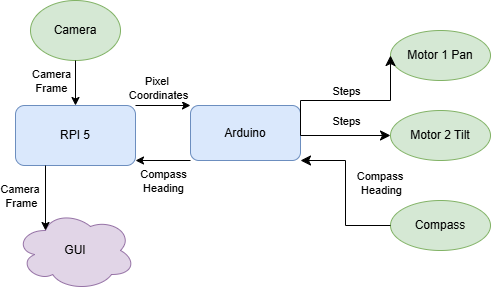
\includegraphics[width=0.5\linewidth]{Figures/Andreas/Flowcharts/Camera_flowchart.png}
    \caption[Communication flowchart]{Flowchart showing the communication bewteen devices}
    \label{fig:placeholder}
\end{figure}

\begin{figure}[H]
    \centering
    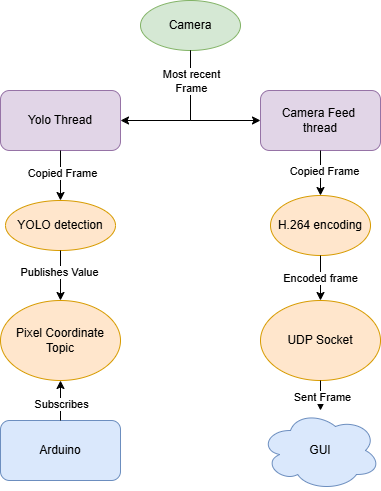
\includegraphics[width=0.5\linewidth]{Figures/Andreas/Flowcharts/Camera_pipeline.png}
    \caption[Camera pipeline flowchart]{Flowchart showing the different threads in the camera pipeline}
    \label{fig:placeholder}
\end{figure}

\section{GUI}
The graphical user interface (GUI) was deliberately engineered to be minimalist and support rapid prototyping, thereby accommodating the evolving requirements that arise throughout the development lifecycle.The design process initiated with a preliminary wireframe that outlined the core components of the GUI page; this sketch subsequently evolved into the wireframe presented in Figure-Add.The GUI was intended to run on a Raspberry-Pi functioning as a web server, which interfaces with the microphone array.

The server was implemented in plain JavaScript to satisfy the storage constraints of the Raspberry-Pi. Docker was employed to construct a reproducible image of the server, enabling rapid testing and updates on an external microcomputer (Raspberry-Pi). The server operates as an HTTPS‑secured service, granting access to the device’s GPS location.

\section{Tests performed}
\subsection{Sound signal acquisition}
The acoustic data signal from the microphones was received using two distinct peripherals on three different STM32 based controllers. The first peripheral used is SAI, and was tested on the  STM32F446 and STM32H753 controllers. The second peripheral tested was the DFSDM which was applied on the STM32F413 MCU. 

\subsubsection{SAI acquisition tests}
The sound acquisition test was conducted by placing the microphone platform seen in Figure~\ref{fig:first_mic_platform}, in the middle of an empty classroom. The test was conducted by one student, whom spoke to the microphones in the distance of around 2 meters. The main objective of the test was to evaluate wether the acquired microhpone signals could be used by the DOA algorithm, which at that stage of the project, was expected to estimate the direction of the strongest sound source.\\

\begin{figure}[h]
        \centering
        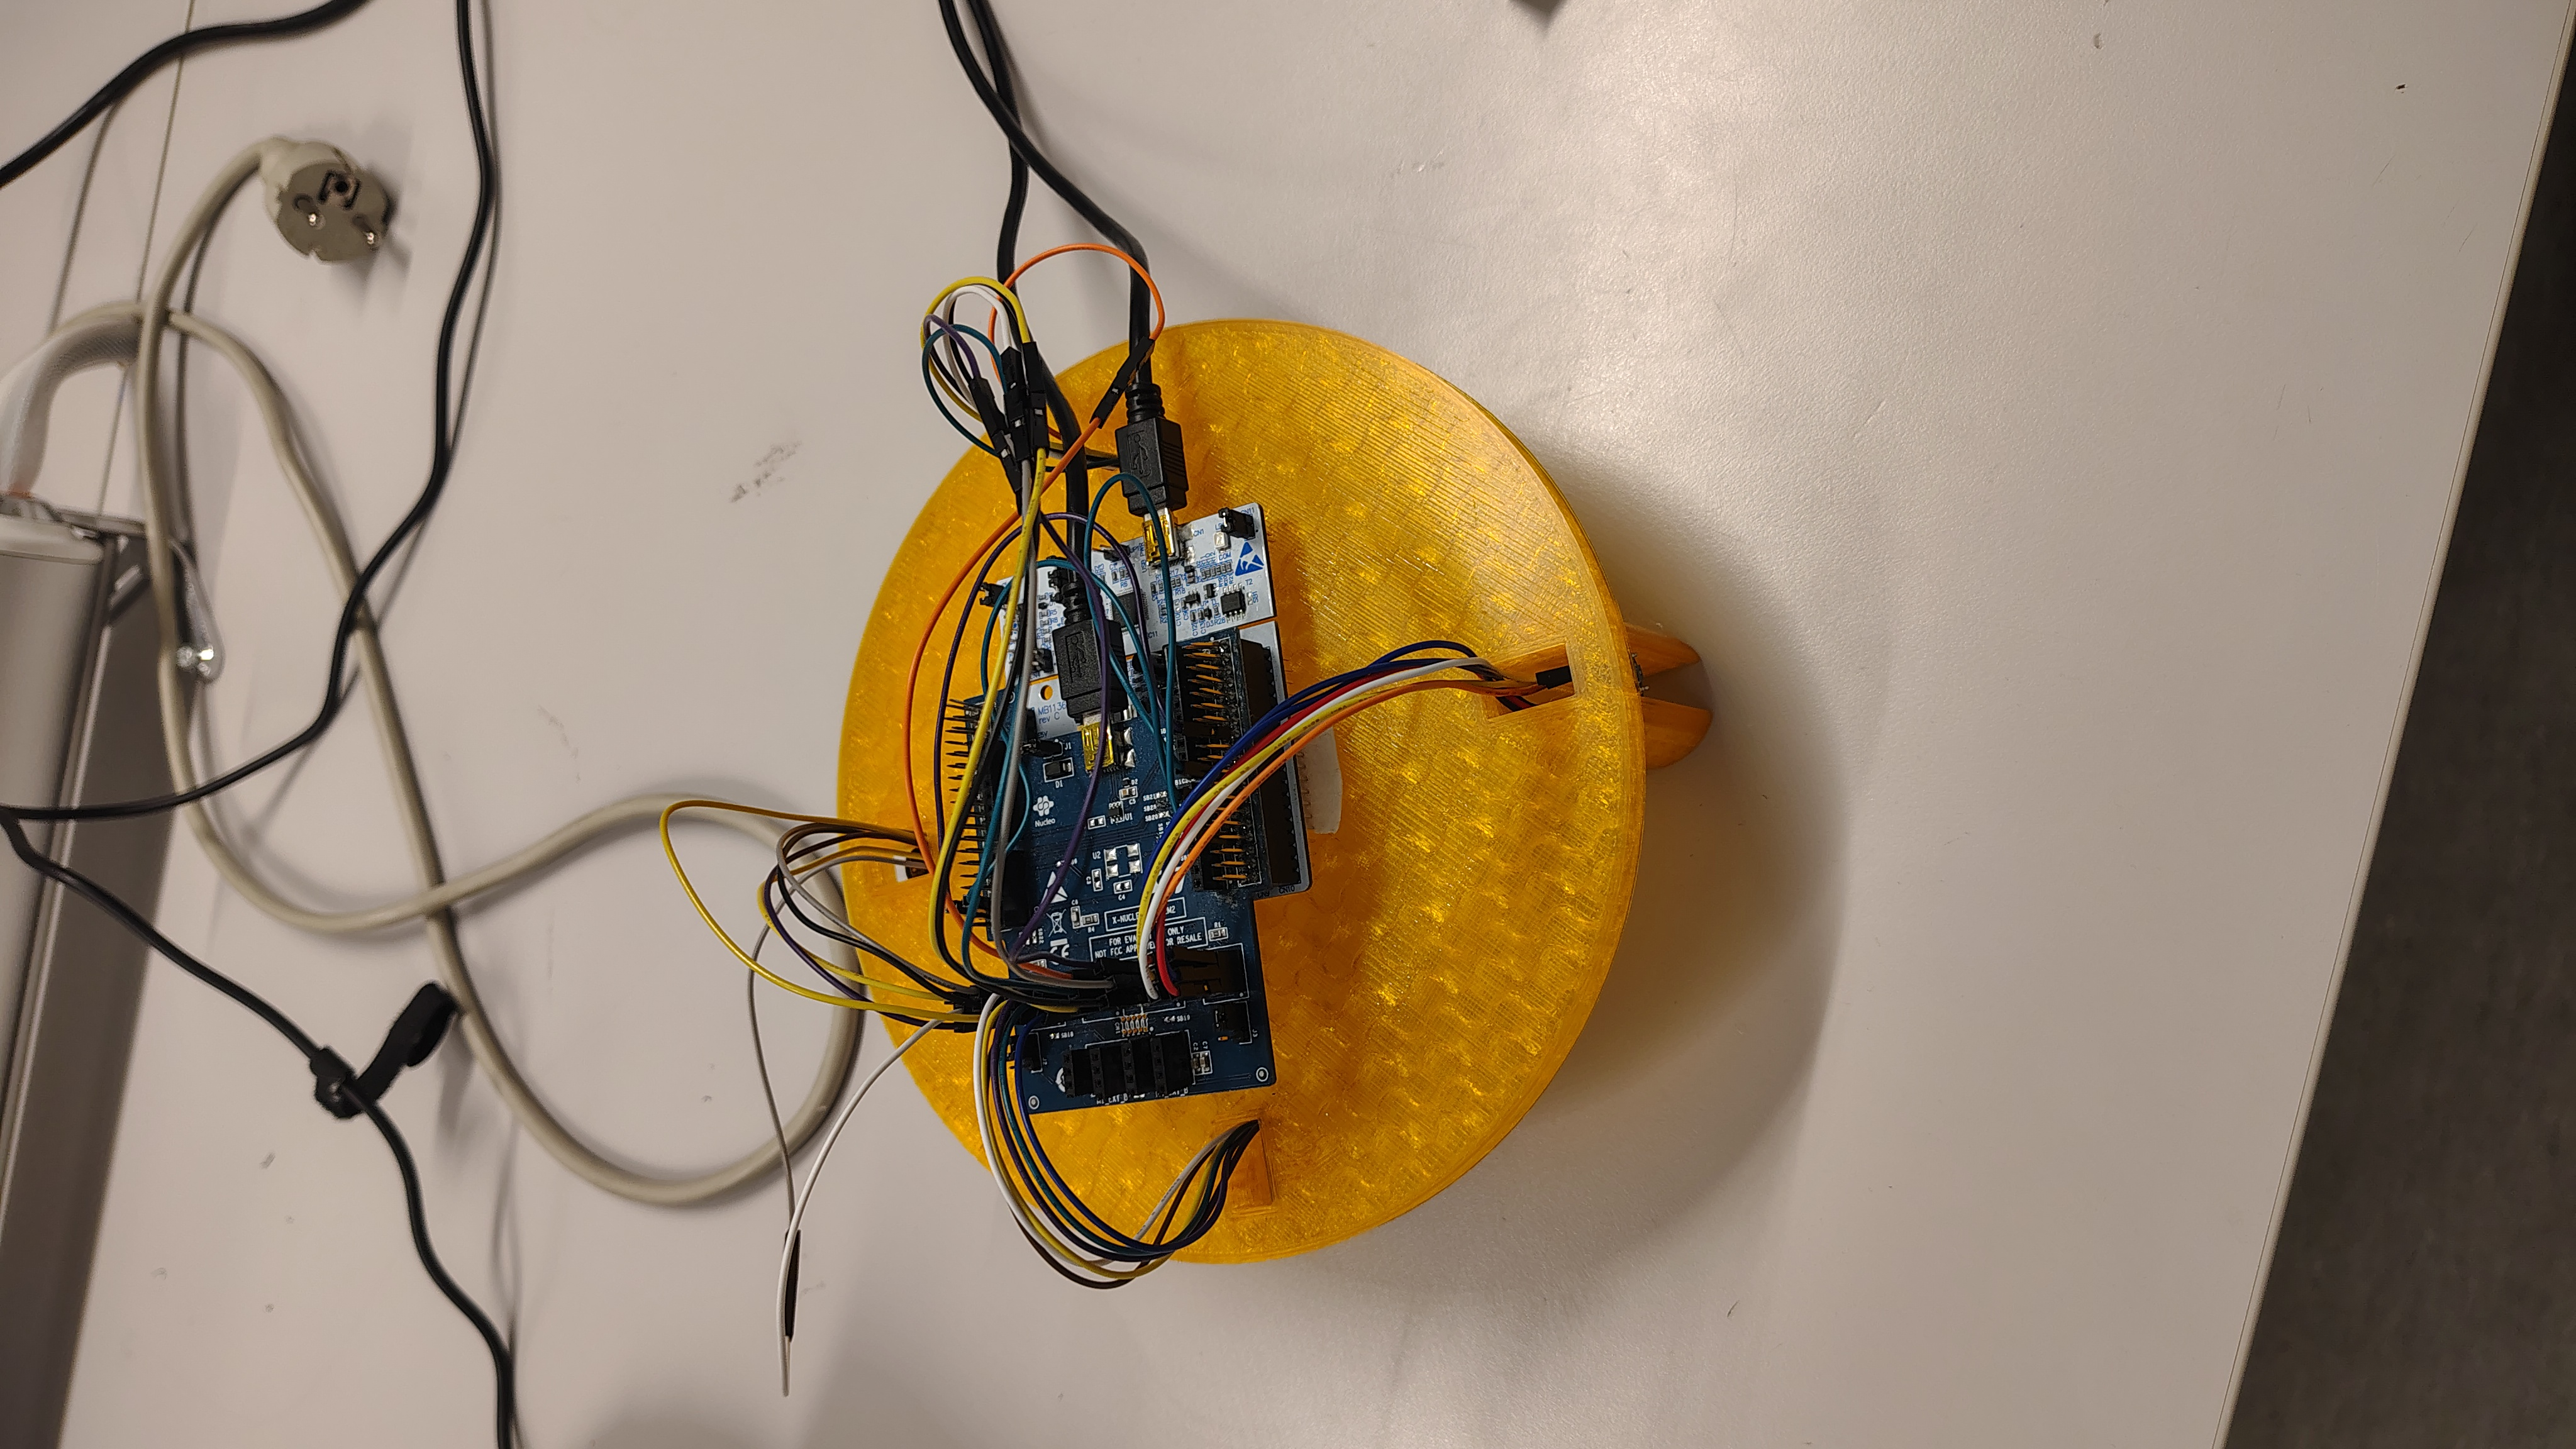
\includegraphics[width=0.5\linewidth]{Figures/IMG_20260220_212107140_HDR.jpg}
        \caption[The microphone first platfrom]{The first microphone platform design used for testing of the sound acquisition pipeline}
        \label{fig:first_mic_platform}
    \end{figure}
\newpage
\subsubsection{DFSDM acquisition tests}
After several trials with the SAI peripheral, the acquisition method was changed from SAI to DFSDM. This also required changing the MCU to the STM32F413, which supported the DFSDM peripheral used in the final implementation. A more detailed explenation of this peripheral change is given in Section~\ref{sec:stm32_models_reasoning}.\\

The DFSDM acquisition test was conducted in the same way as the previous SAI tests, where one student spoke or clapped towards the microphone platform from a distance of approximatley 2 to 7 meters.

\subsection{DOA estimation tests}
Testing of the DOA estimation module was conducted in three different stages
after the DFSDM peripheral was implemented in the system. The purpose of the first stage was to verify whether the system could estimate the direction of the dominant acoustic source under simple test conditions, while the two other stages mainly focused on DOA estimation of the actual drone sounds.

\subsubsection{Stage 1: Human-generated sounds}
The first stage used the human speech and clapping sounds, as the test signals.
These sounds were produced at distances of up to 2 meters from the microphone platform, both in an empty classrom and in a classroom occupied by other students. The test signals were used because they were easy to produce repeatedly ,during testing and made it possible to quickly evaluate the behaviour of the DOA algorithm, before testing it with the drone sounds.

\subsubsection{Stage 2: Recorded drone and drone-like sounds}
The second stage of the testing process used the sound made by a DC-motor supplied by 6V and drawing around 200 mA, and a recorded drone sound taken from Youtube, that can be accessed in: \href{https://www.youtube.com/watch?v=gA7-gb7l3Fc}{The drone sound video from youtube}. The purpuse of this testing stage, was to verify if the system is able to detect the sound made by the drone, or drone like sounds.\\

The test involving the drone video, was conducted by placing the mobilephone in the distance of around 7 meters away from the station, and at an angle of approx. -90 degrees relative to the station. The volume on the phone was turned to the maximum, while playing the drone video for the first test, and was later reduced to approx.50\% and 5\%. \\

Additionally the root-mean-square or simply (RMS) value was used as a relative measure of signal magnitude, as it seamed to be a more suitable in  describing the varying signal than a simple average, based on \cite{openlearn_rms}. The code used to generate the RMS can be seen in Code~\ref{lst:rms}, and is based on \cite{oxford_rms}.\\

\newpage

\begin{lstlisting}[style=pythonstyle, caption={logic for calculating the RMS per channel}, label={lst:rms}]
rms_per_channel = np.sqrt(np.mean(df**2))
\end{lstlisting}

%The energy level in db, was found by using Equation~\ref{eq:log_phone_volume}.

%\begin{equation}
%    \label{eq:log_phone_volume}
%    Relative \space level= 20\log_{10}(\frac{level_{test}}{level_{100}})
%\end{equation}

\subsubsection{Stage 3: Live drone test}
The third and the last stage of the DOA estimation testing, was conducted by using the drone present at the visualization lab. The first series of tests did not involve the use of the ML or the camera, and the setup was as seen in Figure~\ref{fig:doa_3_stage_no_camera}. Where the bottom part of the tower, with the microphones mounted on it, was placed in the middle of the laboratory. \\

The system was first tested without the drone present, in order to observe the background noise level in the laboratory, which would be later used as a baseline, to compare the frequency content of the room noise, with the frequency content produced when the drone was flying.


\begin{figure}[h]
    \centering
    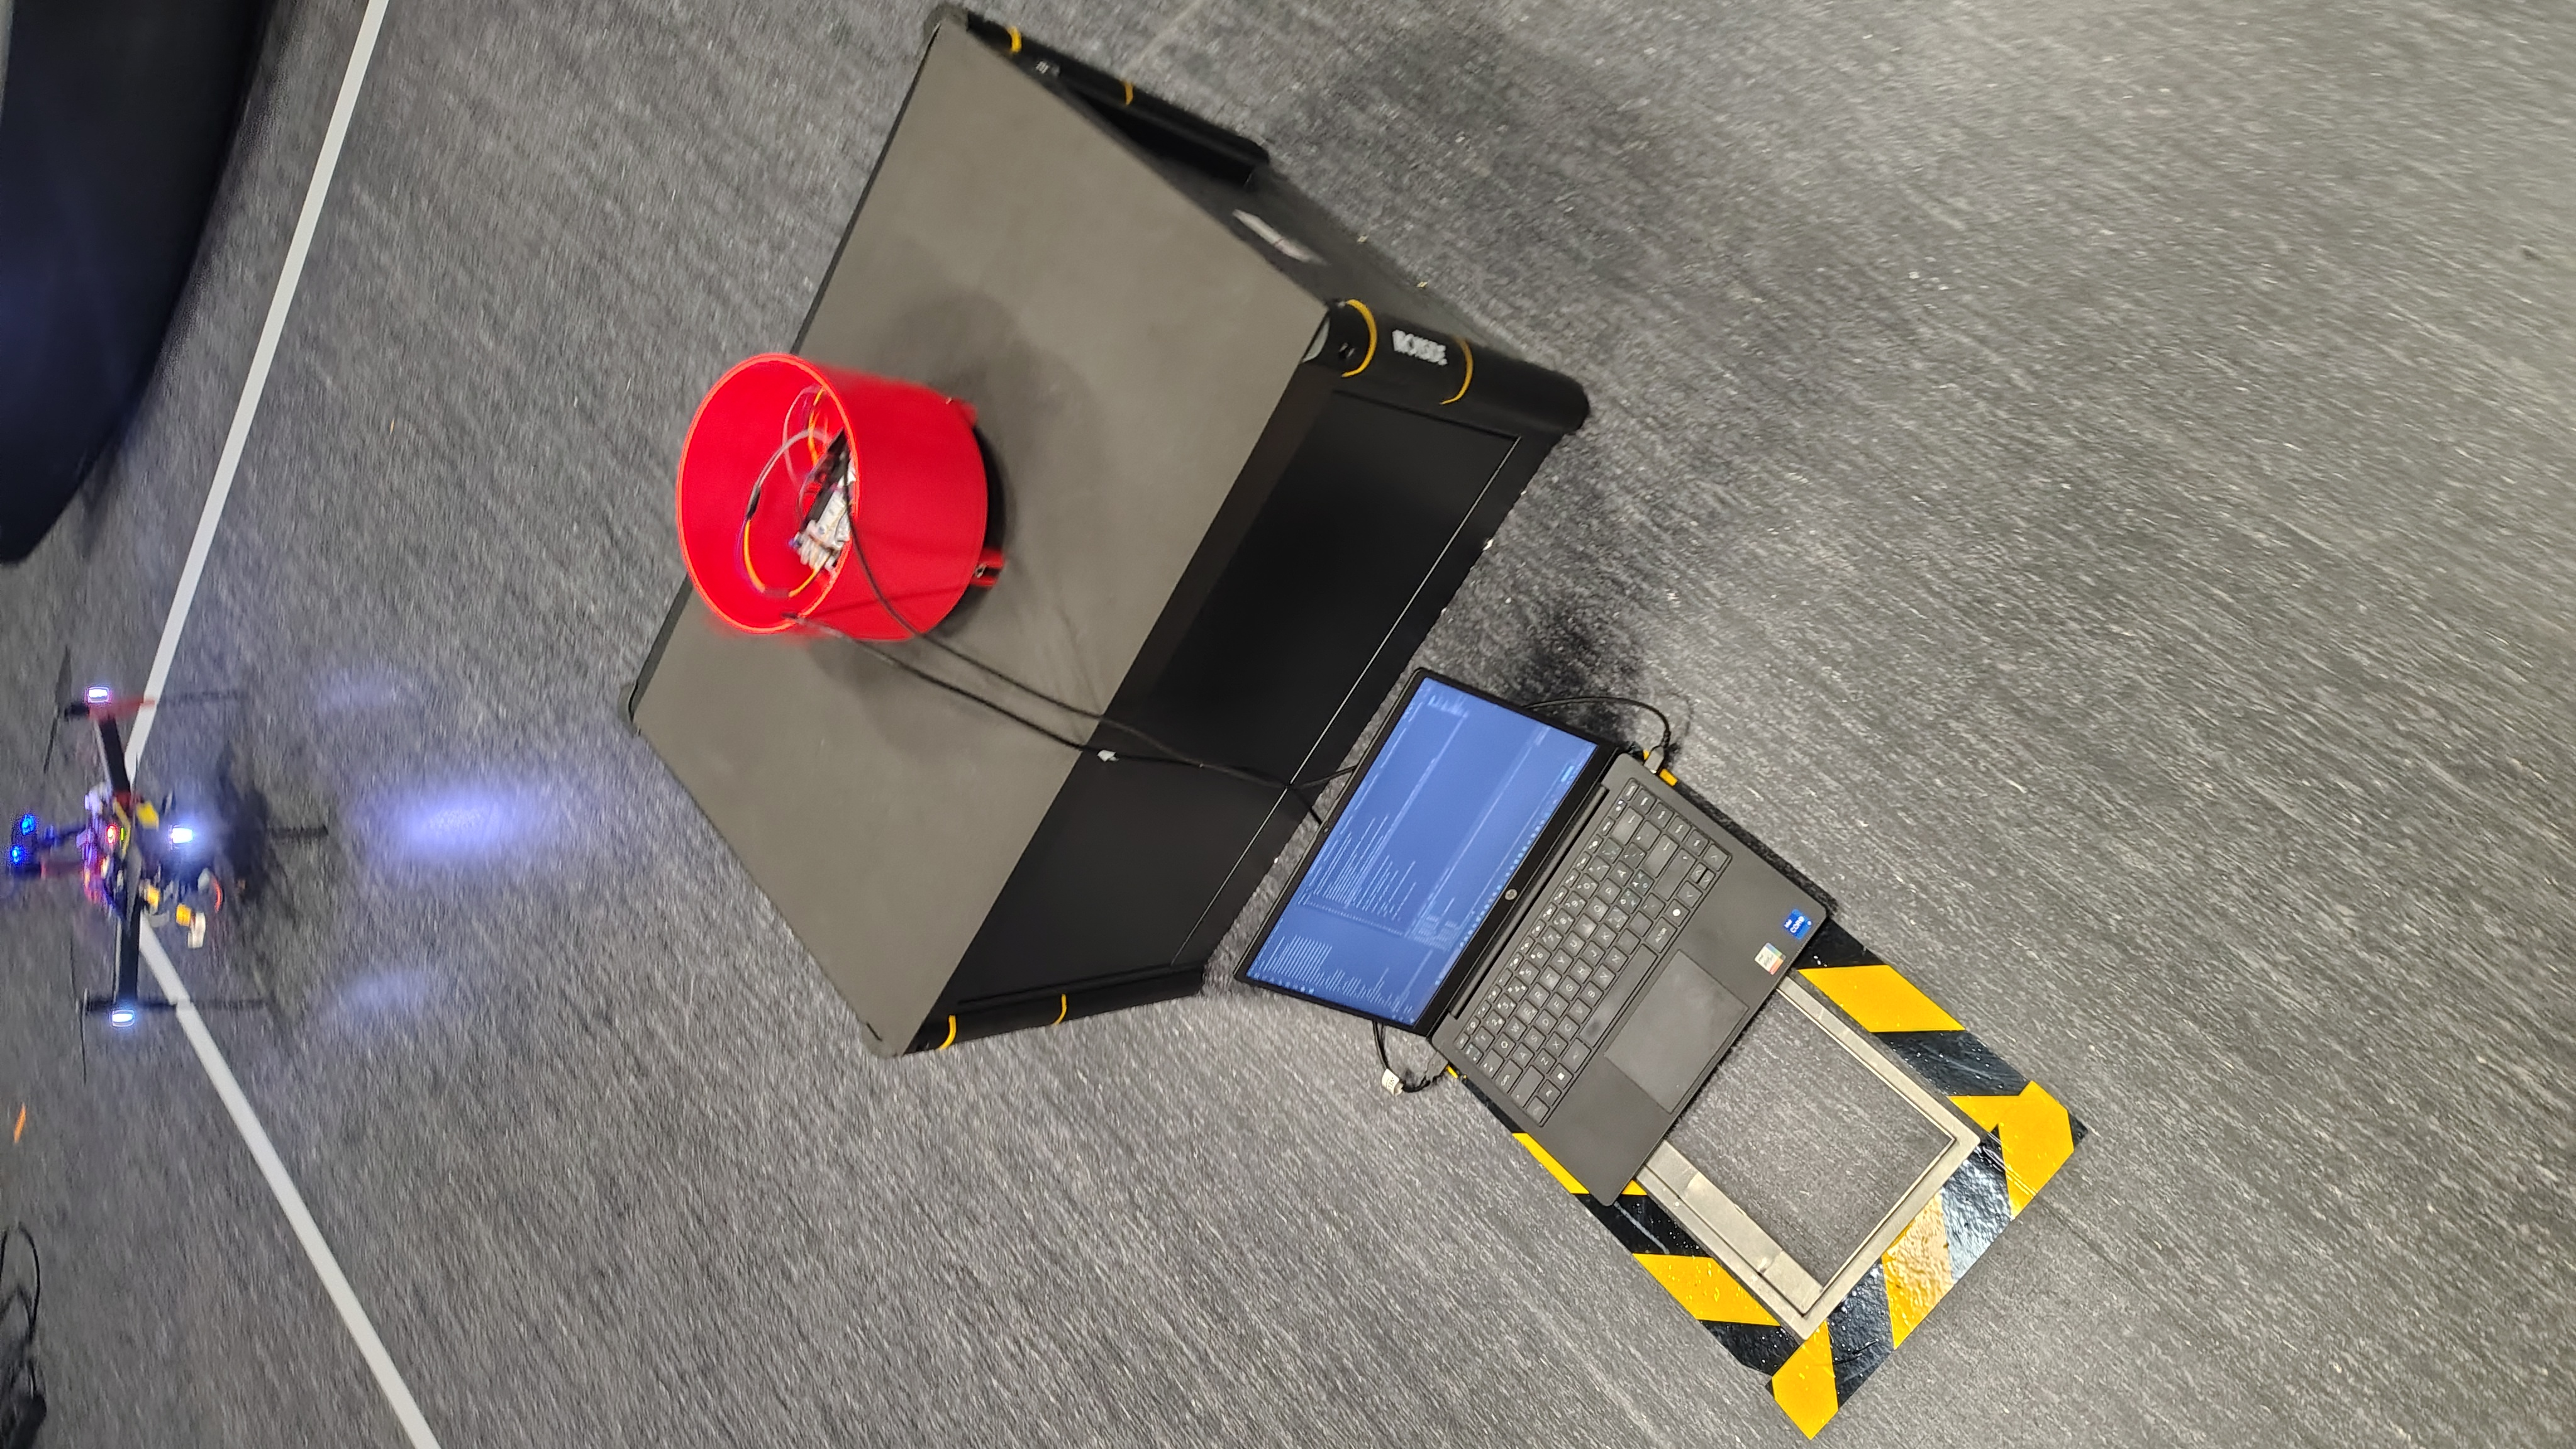
\includegraphics[width=0.5\linewidth, angle=-90]{Figures/1000001927.jpg}
    \caption{The first test in the third stage of the DOA estimation testing}
    \label{fig:doa_3_stage_no_camera}
\end{figure}

The next test involved the use of the live-drone which was circulating around the tower, while the system was processing the acquired sound to estimate the DOA.\\
\newpage
The final test was conducted after the ML-algorithm togheter with the camera was implemented in the system, where the test enviroment would be the same as for the previous tests as seen in Figure~\ref{fig:doa_3_stage_setup}.\\ 

\begin{figure}[h]
    \centering
    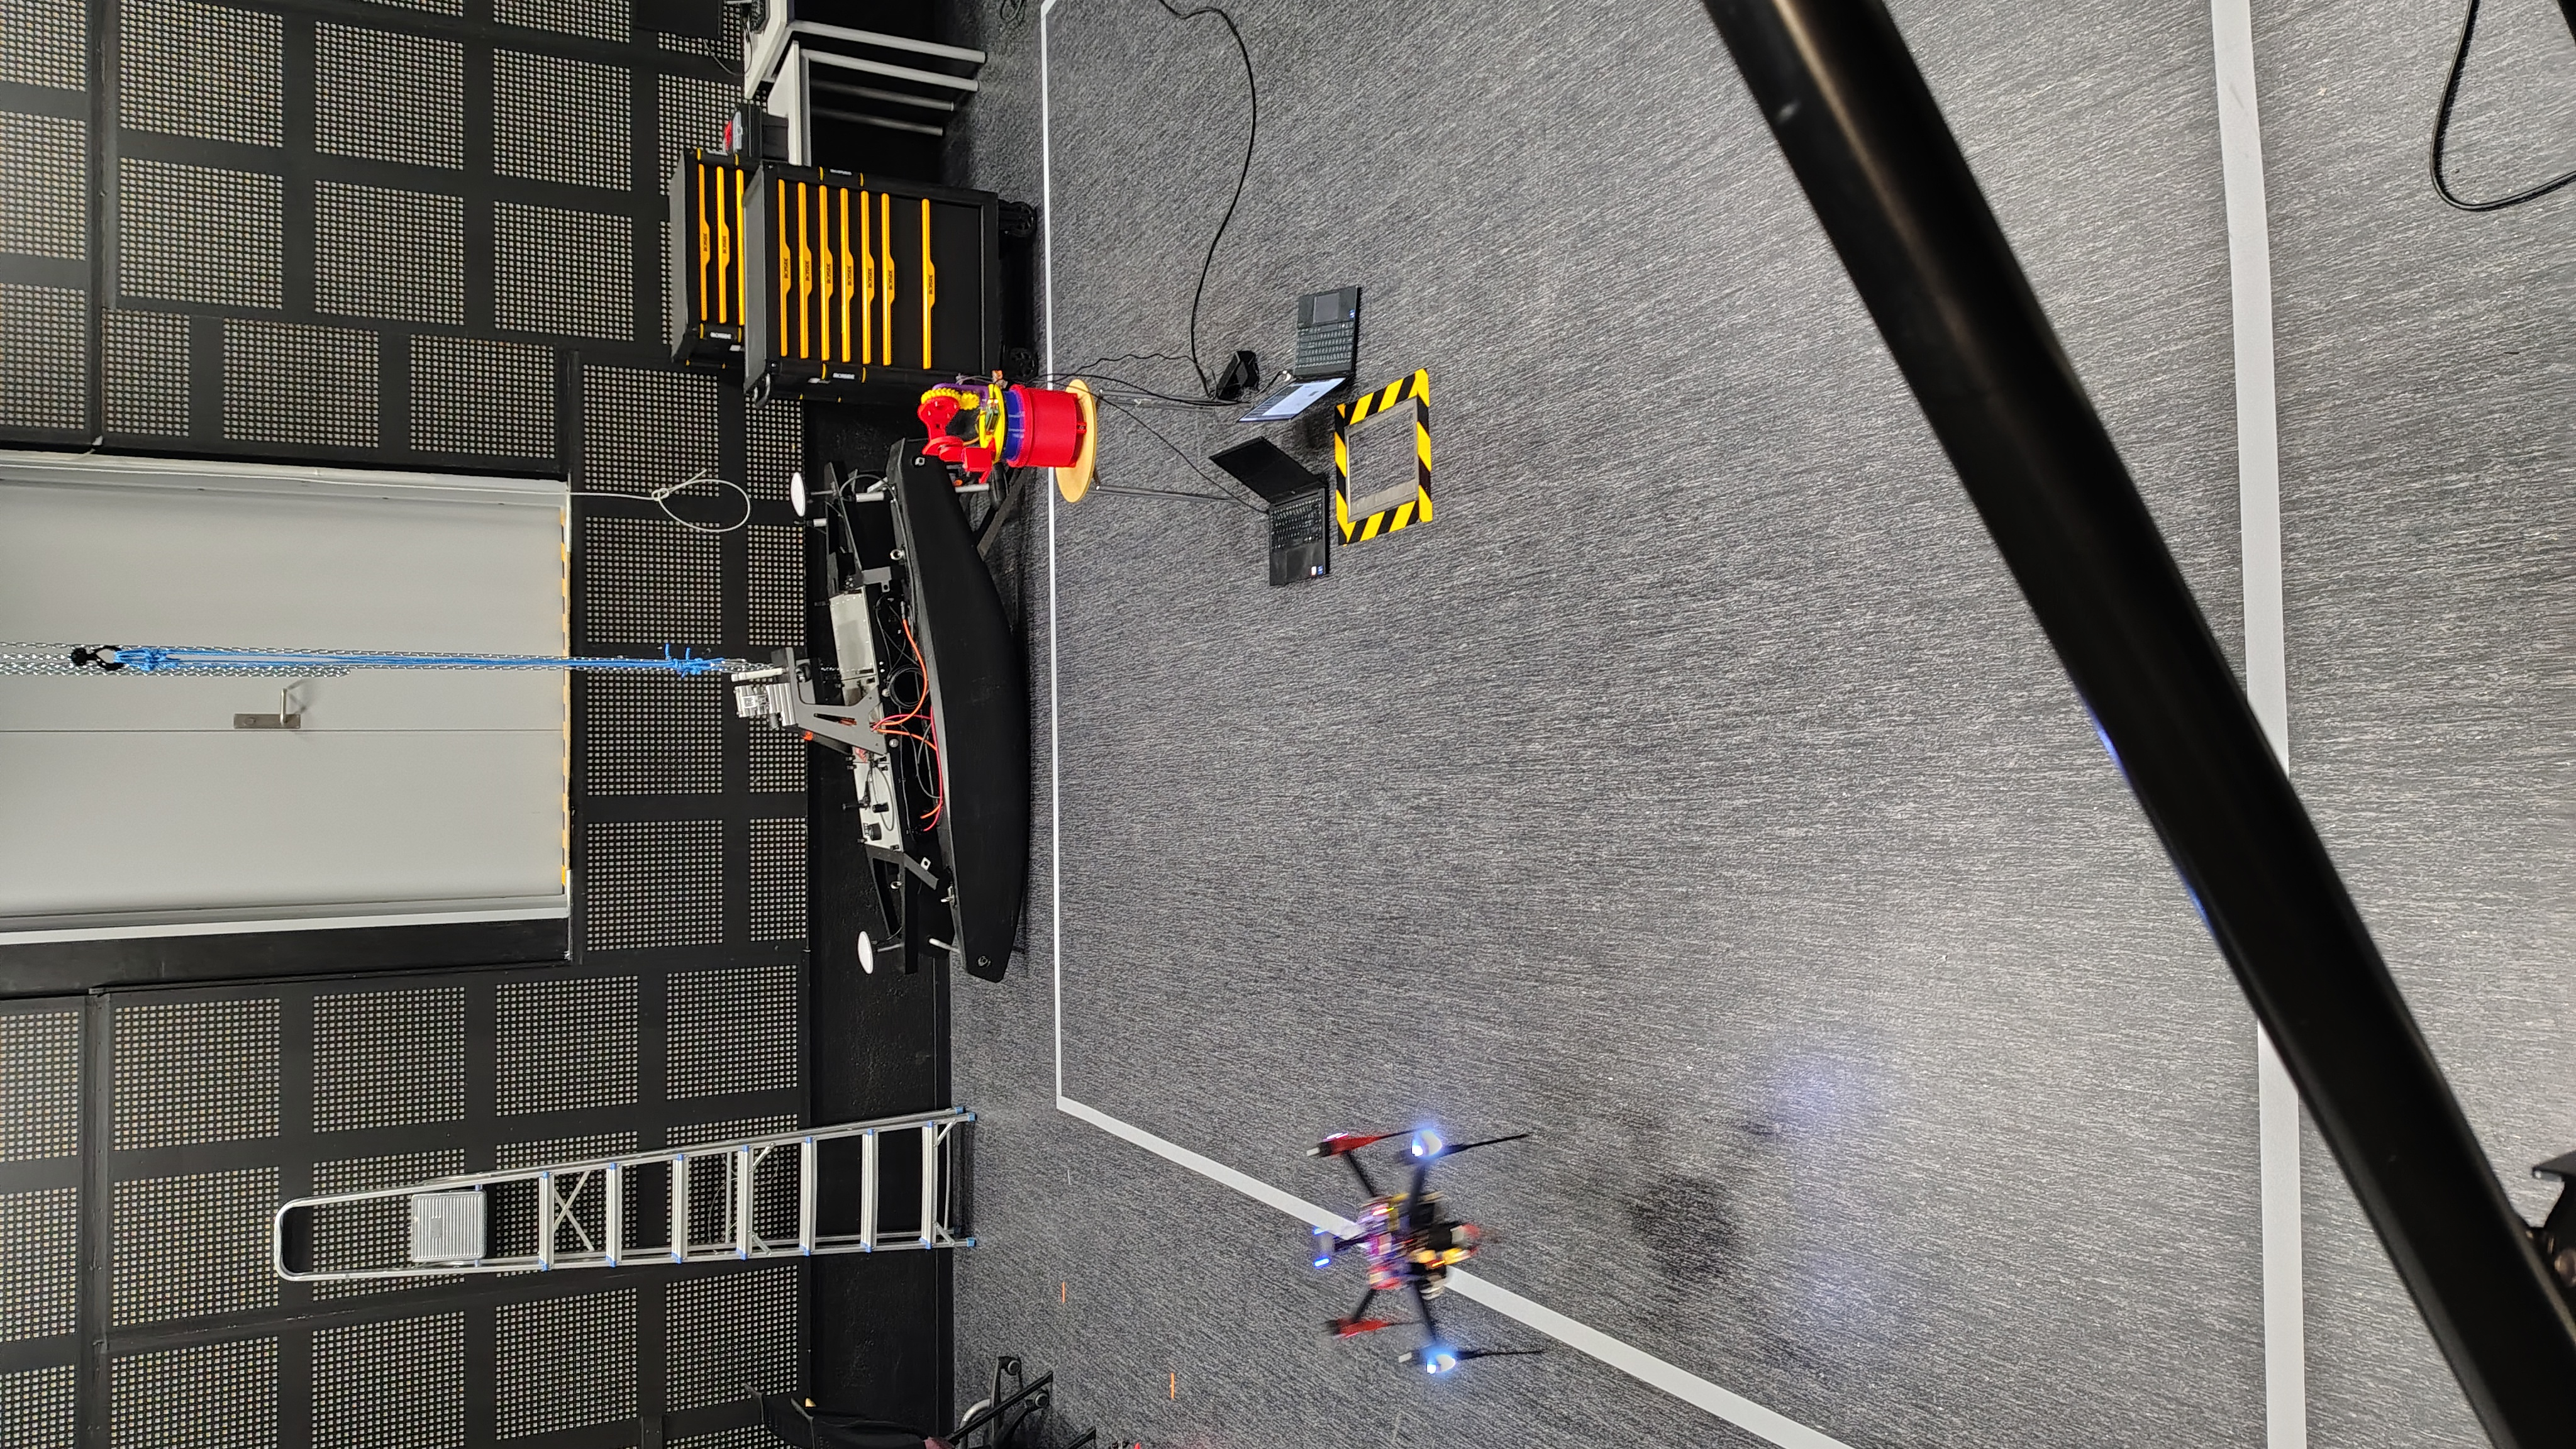
\includegraphics[width=0.5\linewidth, angle=-90]{Figures/IMG_20260514_115338104_HDR.jpg}
    \caption{Setup for the third DOA testing stage}
    \label{fig:doa_3_stage_setup}
\end{figure}
\newpage
The ML was tested by letting the system record the sound without the drone present. The system was expected to return the "Not a drone" flag, which would not allow for the DOA estimation to be conducted, and later the drone would be flown, so that the ML could return the "drone" falg and allow for DOA estimation.\\

After the ML algorithm was verified, the final test was conducted, where the drone was flawn around the tower, in varying distance but not outside the safety area designated in the laboratory ,due to the safety conserns. The system was expected to accurately produce a DOA estimation as it was proven possible in the previous tests. Since the drone was to be in constant circulation around the tower, it was expected that the DOA estiamtion will lag behind the drone with a lag of atleast 1 second, due to the duration of the recorded sound, and some additional overhead caused by the other modules in the system.\\  

\subsection{Hardware test}

In order to test the hardware requirements of running a YOLO model on a raspberry pi 5 a stress test was performed while logging the CPU usage, temperature as well as the RAM usage of the system. Interference time was also measured while the YOLO model was run by the system. The test was performed while utilising the HAILO chip, as well as running the model on the CPU only. 

\subsection{Project Management}
The Development team employed the Scrum framework to organise the work. The project was split into bi-weekly sprints. At the end of each sprint the team performed a sprint-review, during which the team went over what was accomplished and what needed to be done by the next sprint.

The product owner, Erlend-Magnus-Lervik-Coates (NTNU-Dronelabben), participated in all review meatings and some planning meatings. The backlog was managed with Github Issues, which served as the source of user stories, bug reports and task assignments.





%\section{Signal Processing Implementation}
% Maybe split into GCC and MFCC?
% ADD the influence that SNR has on confidence of a segment in gcc!
% “A confidence measure based on the ratio between the correlation peak and the average energy in the segment is used to discard unreliable frames. This can be interpreted as a local SNR estimate.” ? 
%    \subsection{Frame length}
%    \subsection{Windowing}
%    \subsection{FFT size}
%    \subsection{PHAT implementation}
%    \subsection{Sub-sample interpolation}
%    \subsection{Confidence filtering}

%\section{Feature Extraction}
%    \subsection{MFCC}
%    \subsection{ML}
\clearpage

\chapter{Results}
The project is an open-source, real-time system that uses audio and visual data to detect and locate drones. Continuous audio streams are captured by a microphone array and processed by a convolutional neural network (CNN) classifier, which determines whether the audio signature contains a drone. When a positive detection occurs a python script calculates the angle of the audio signature then sends it to a web-based graphical user interface(GUI). The system captures a video stream that is processed by a YOLO algorithm then sent to the GUI. The GUI visualises the angle on a polar map and integrates the live video feed. 
\begin{figure}[H]
    \centering
    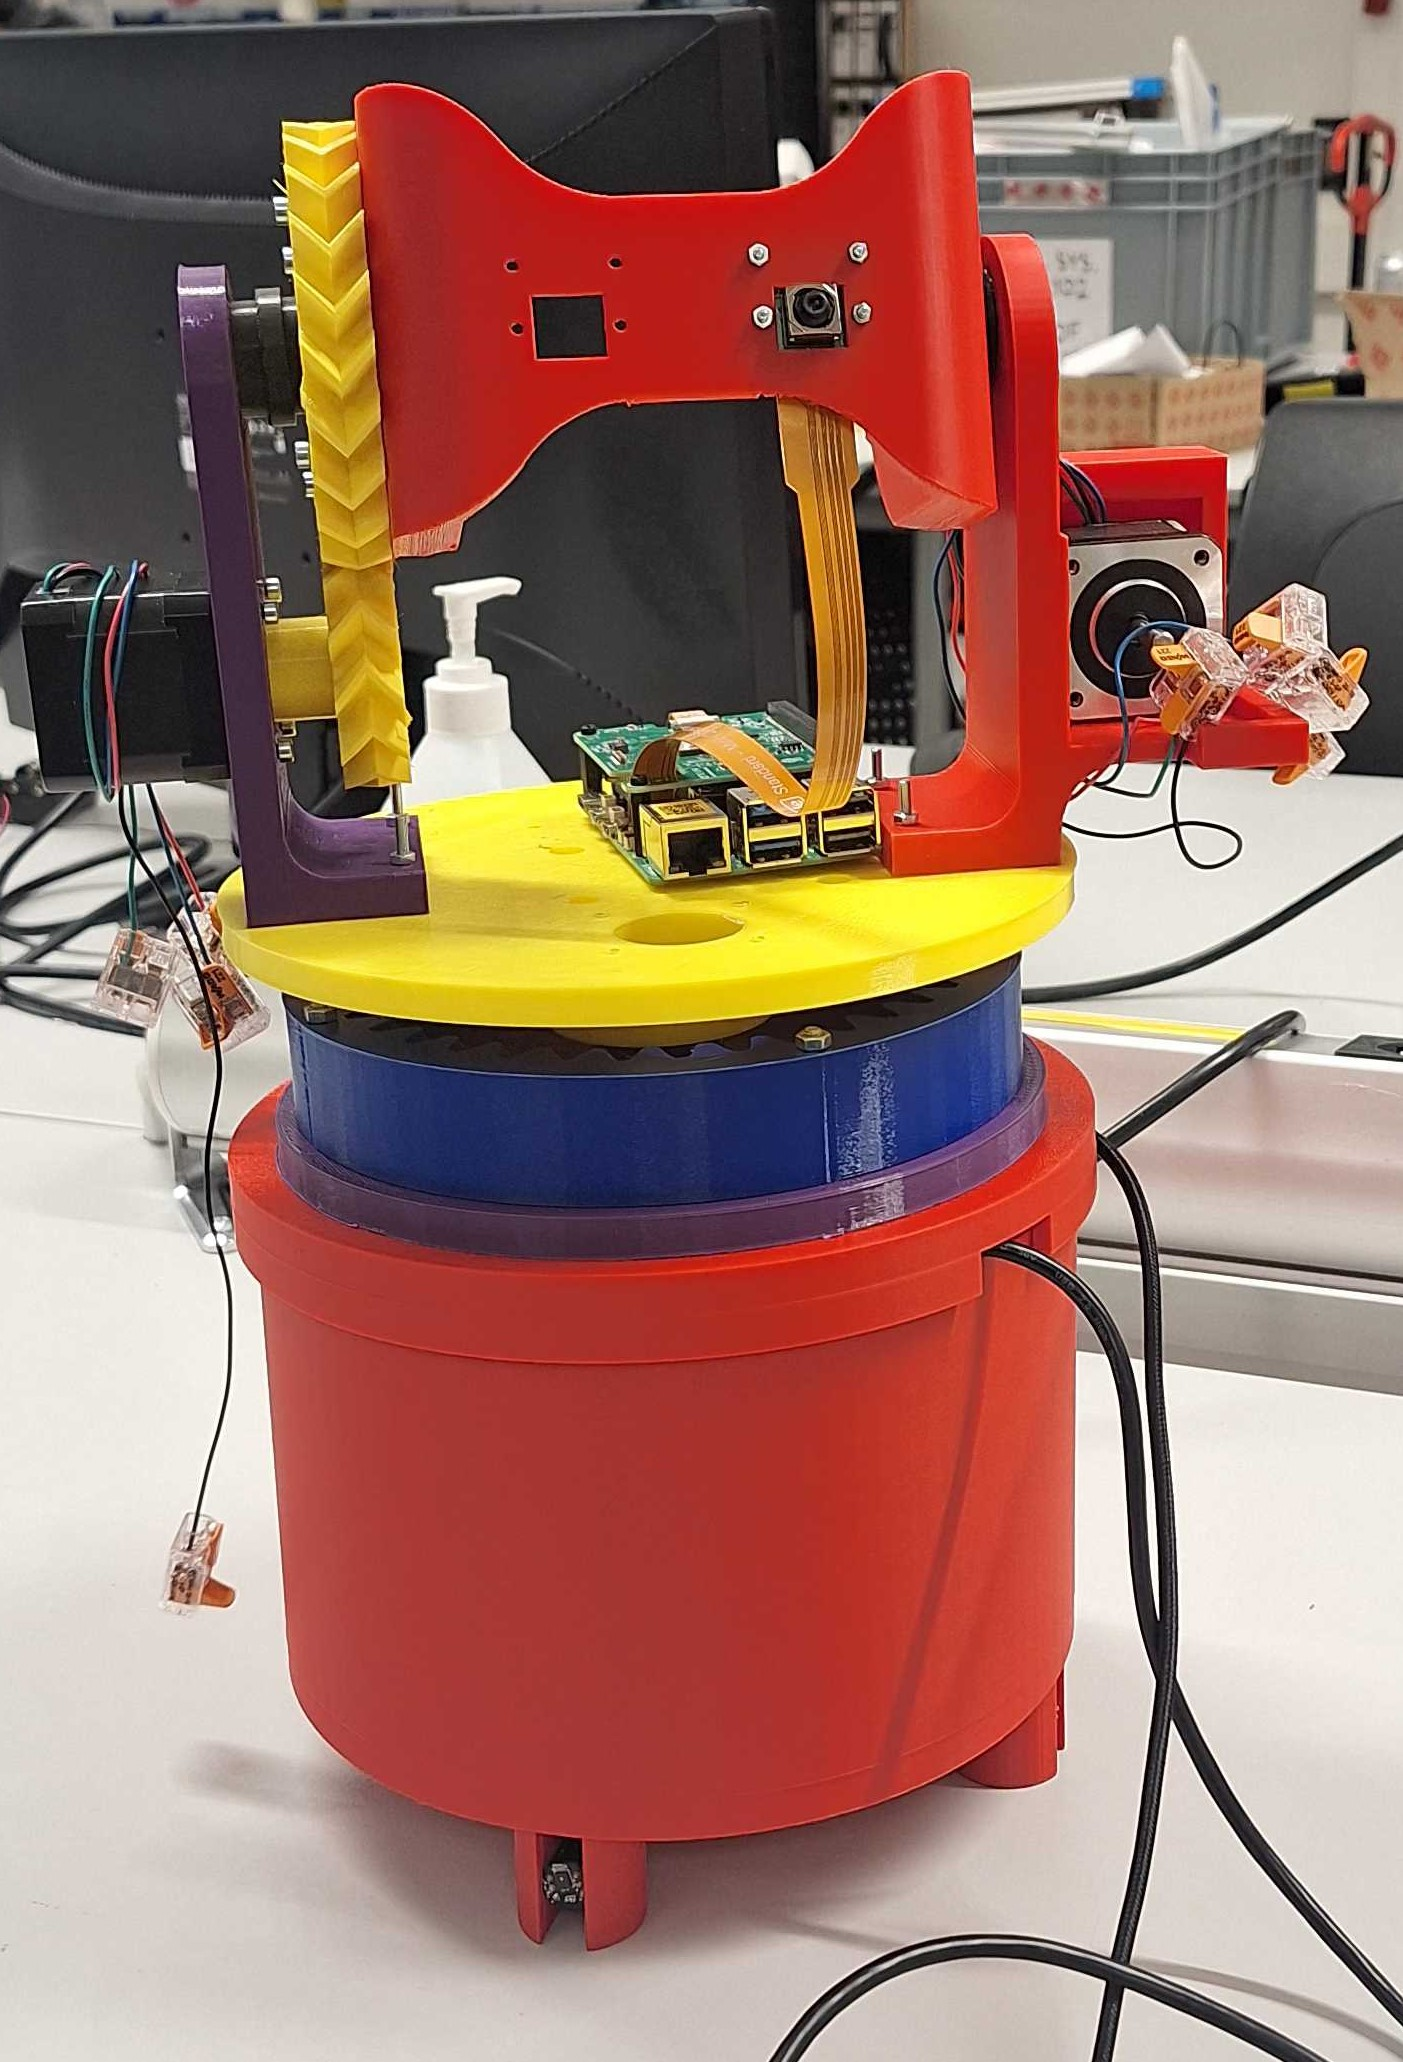
\includegraphics[width=0.5\linewidth]{Figures/Brage/FullSystem.jpg}
    \caption{Picture of the finished system}
    \label{fig:placeholder}
\end{figure}

\begin{figure}[H]
    \centering
    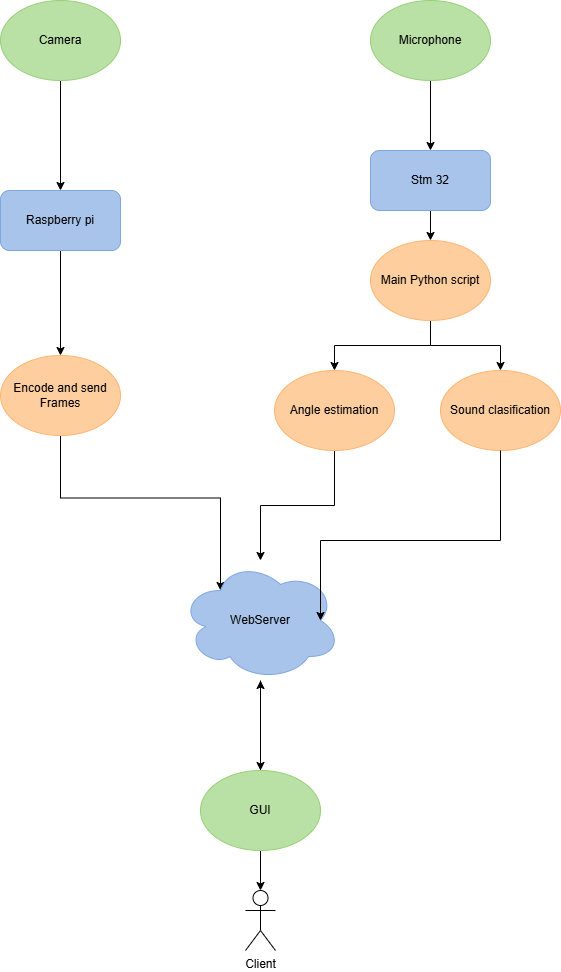
\includegraphics[width=0.5\linewidth]{Figures/Brage/FlowcahrtFullSystem.drawio.png}
    \caption{Low level flow chart of system}
    \label{fig:placeholder}
\end{figure}

\section{Sound signal acquisition results}
    \subsection{SAI acquisition test results}
    The SAI acquisition test resulted in the signal shown in Figure~\ref{fig:pcm_sai}.
    During the test, the azimuth estimation appeared random, which led to the troubleshooting of the acquisition pipeline. The troubleshooting results indicated, that the problem seamed to be related to data leakage or incorrect channel separation between the micropohones sharing the same line. This was supported by high correlation values between microphone pairs connected to the same line as shown in Figure~\ref{fig:corr_sai}. In addition, when one microphone from a pair was disconnected, the received signal still contained data in the channel representing the disconnected microphone. A more detailed explenation of this troubleshooting process is given in Section~\ref{sec:troubleshooting_sound_acquisition}.\\
    
    Despite the observed mixing between microphone channels, the signal was still sufficient to reconstruct understandable audio from the recording. The reconstructed WAV file contained a large amount of noise, but the speech produced by the student could still be understood. The signal was also still usable for MFCC extraction, althoguh Figure~\ref{fig:mel_spec_sai_test} shows that the speech-related spectral components were mixed with a considerable amount of high frequency noise. However, the signal quality was not sufficient for reliable DOA estimation, and additional filtering or correction would have beed required before using the signal for further analysis.

    \begin{figure}[h]
        \centering
        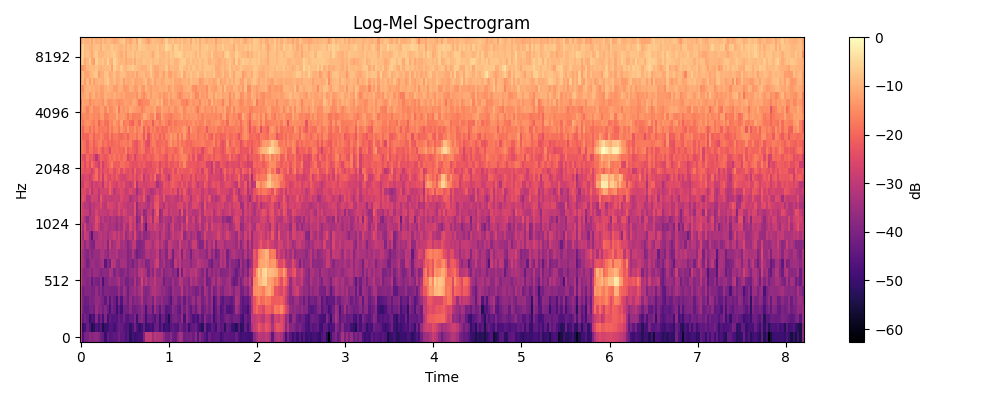
\includegraphics[width=1\linewidth]{Figures/mel-spec.png}
        \caption[Mel-spectrogram for SAI testing]{A Mel-spectrogram produced during the speech test using SAI}
        \label{fig:mel_spec_sai_test}
    \end{figure}
    
    \newpage
    \subsection{DFSDM acquisition test results}
    The resulting PCM signal acquired during the DFSDM test is shown in Figure~\ref{fig:pcm_dfsdm}. Compared with the SAI acquisition, the DFSDM signal appeared more stable and contained less visible noise. This was also reflected in the Mel-spectrogram shown in Figure~\ref{fig:mel_spec_dfsdm_test}, where the clapping-related frequency components were more clearly visible.\\

    The DFSDM signal also resulted in more consistent DOA estimation during the initial speech, and clapping-based tests. This with addition of the correlation matrix in Figure~\ref{fig:corr_dfsdm} indicates that the problem of data leakage has not occured. Based on these results, the DFSDM peripheral was selected as the final method for microphone data acquisition and was used in the lated tests involving recorded drone sound and the live drone.

\begin{figure}[h]
    \centering
    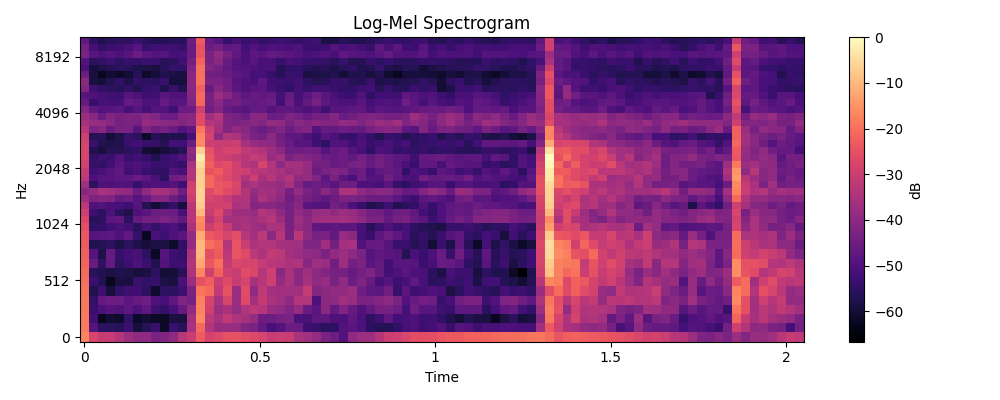
\includegraphics[width=1\linewidth]{Figures/Debug_mel_spectrogram1777801860.6435578.png}
    \caption[Mel-spectrogram for DFSDM testing]{A Mel-spectrogram produced during the clapping test using the DFSDM}
    \label{fig:mel_spec_dfsdm_test}
\end{figure}

\begin{figure}[H]
    \centering
    \begin{subfigure}[b]{0.48\textwidth}
        \centering
        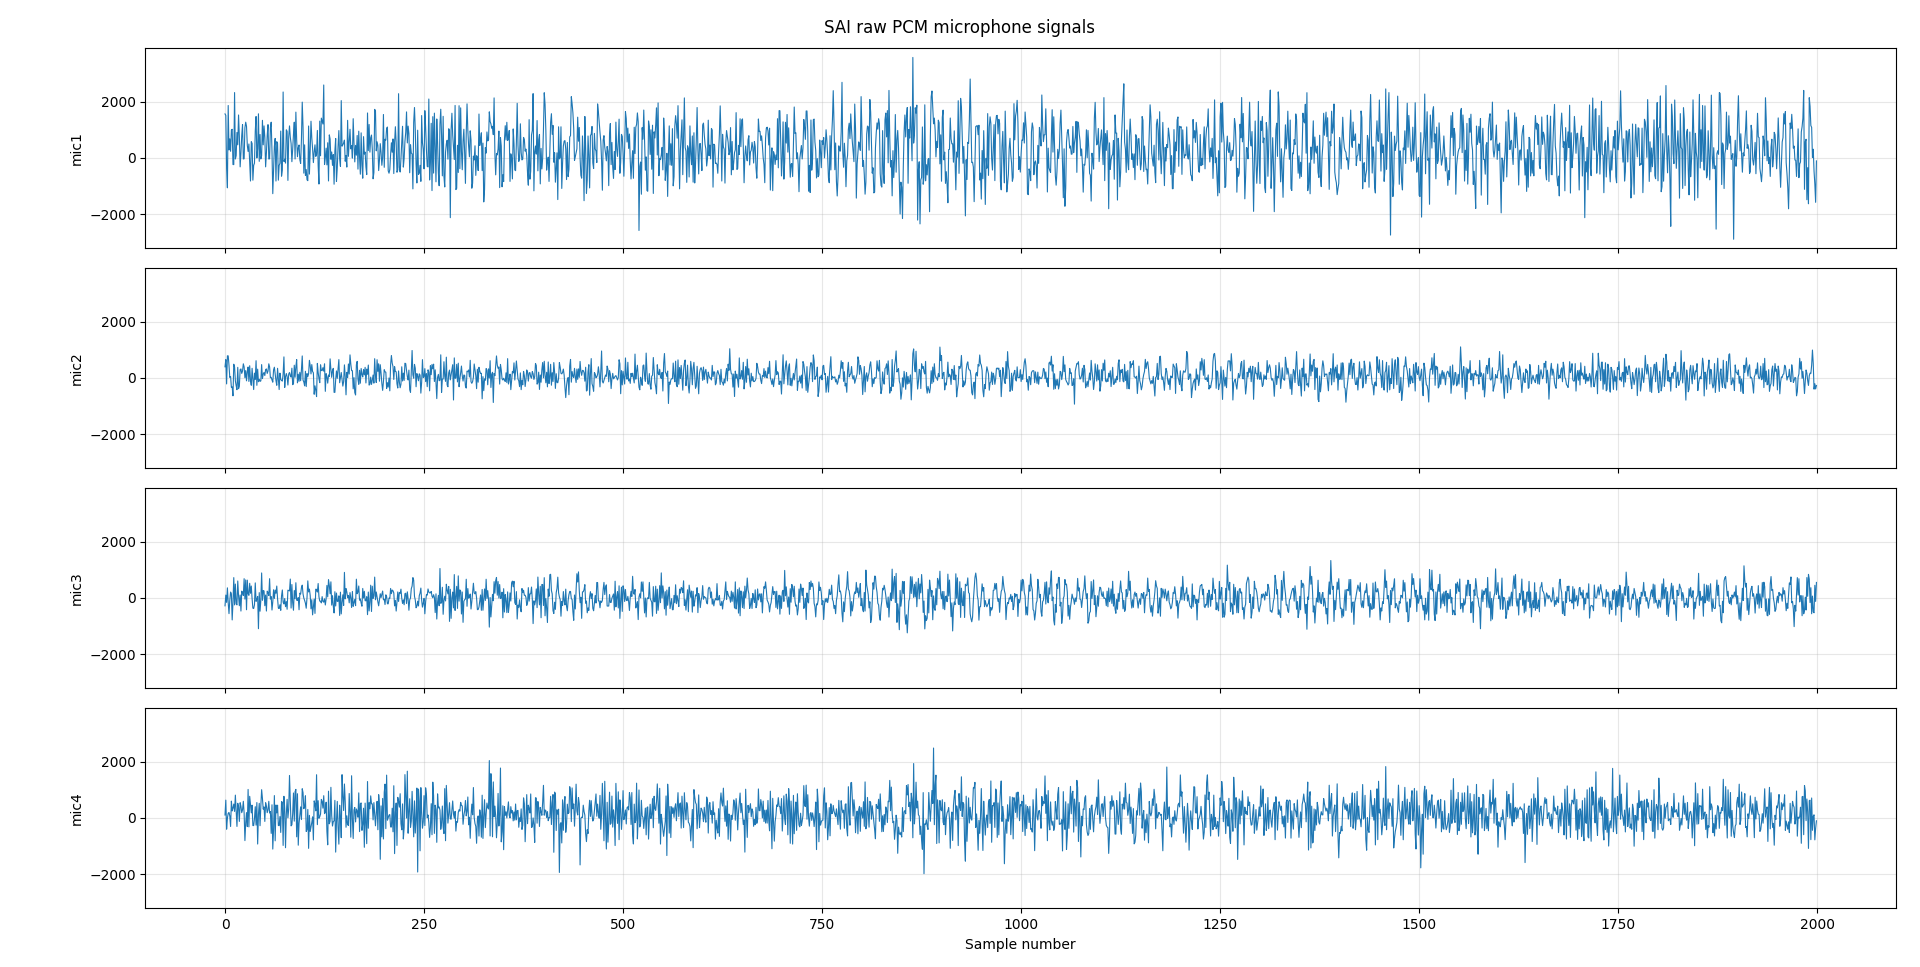
\includegraphics[width=\textwidth]{Figures/sai pcm figure.png}
        \caption[PCM when using the SAI]{PCM values transferred from MCU when acquiring PDM values through SAI }
        \label{fig:pcm_sai}
    \end{subfigure}
    \hfill
    \begin{subfigure}[b]{0.48\textwidth}
        \centering
        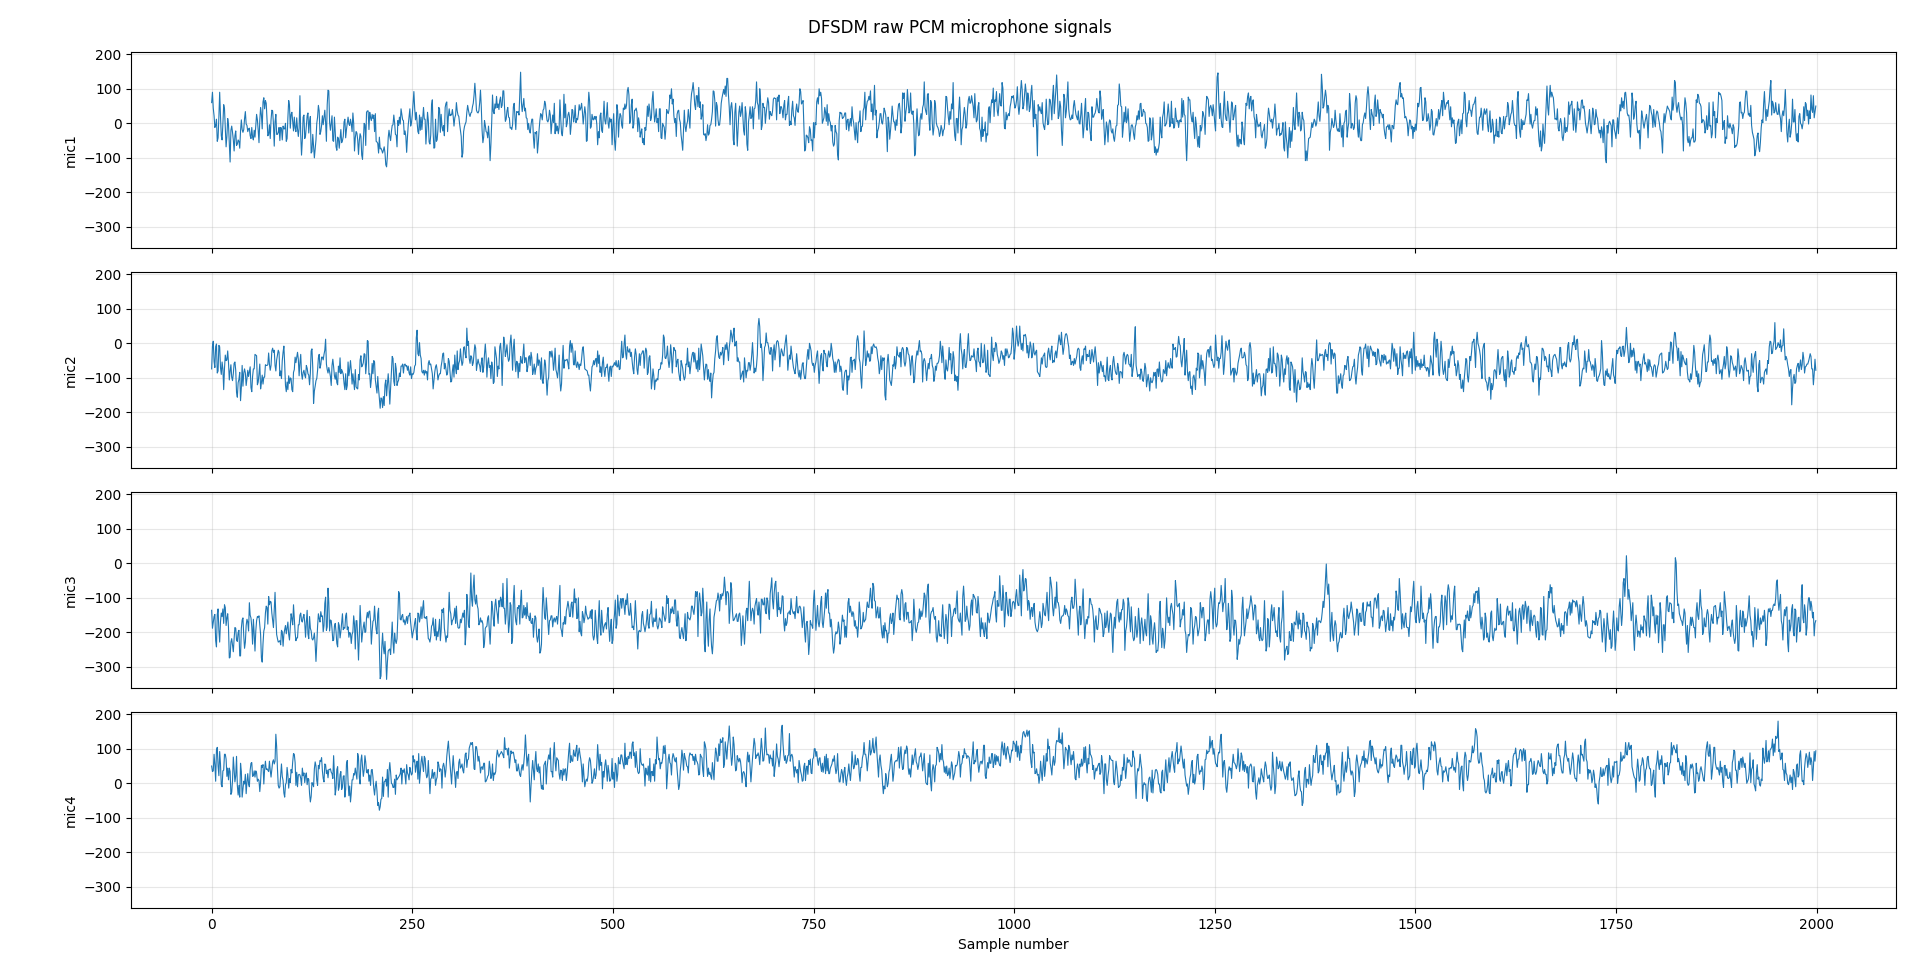
\includegraphics[width=\textwidth]{Figures/dfsdm pcm figure.png}
        \caption[PCM when using the DFSDM]{PCM values transferred from MCU when acquiring PDM values through DFSDM }
        \label{fig:pcm_dfsdm}
    \end{subfigure}
    \caption{Signals received by using the SAI amd DFSDM peripherals on STM32}
\label{fig:dfsdm_sai_signals}
\end{figure}

    \subsection{Comparison between SAI and DFSDM}
    As presented in the previous sections, the signals acquired using SAI and DFSDM differed considerably, even though the tests were performed with similair acoustic input signals. To quantify the difference between the two acquisition methods, the standard deviation was calculated for each microphone channel.\\
    
    The standard deviation was used to describe how much the measured PCM values deviated from the mean value of the signal. A higher standard deviation means that the samples vary more around the mean, which might indicate the presence of stocastic noise components in the signal, or the irregularity of the desired signal itself, assuming that the measured sound is similair between the tests. As shown in Figure~\ref{fig:std_sai_dfsdm}, the signal acquired using SAI had a significantly higher standard deviation than the signal acquired using DFSDM. Additionaly after the wav conversion has occured, it was clearly hearable that the DFSDM acquird signal contained much less noise. This supports the observation that the SAI signal contained larger irregular variations in the PCM values. \\
% move it? 
    The lower STD of the DFSDM signal is likely related to the internal filtering and decimation performed by the DFSDM peripheral. Unlike the SAI setup, the DFSDM peripheral converts the PDM stream to PCM using the configured sinc3 filter. This filter attenuates parts of the high-frequency components present in the signal before the PCM samples are produced. This likely contributed to the lower standard deviation observed in Figure~\ref{fig:std_sai_dfsdm}.\\

    \begin{figure}[h]
        \centering
        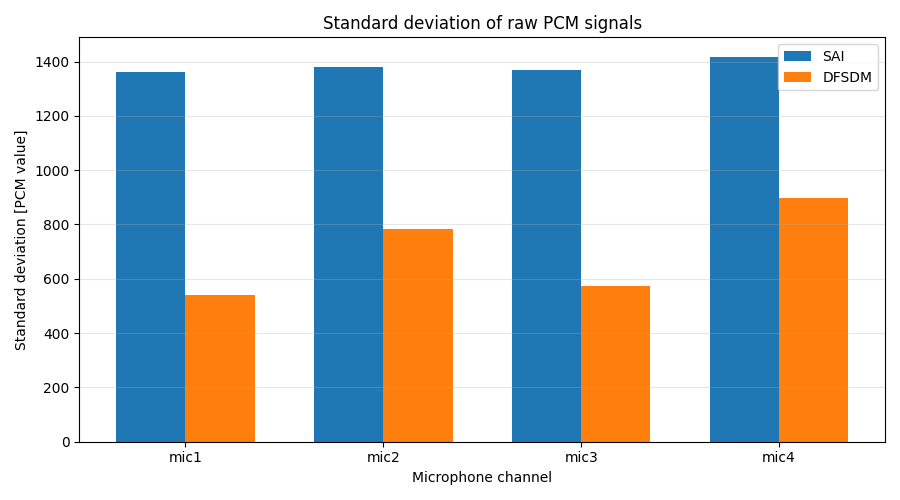
\includegraphics[width=0.5\linewidth]{Figures/std_sai_dfsdm.png}
        \caption[Std comparison of SAI and DFSDM]{Std of the signals gathered with SAI and DFSDM}
        \label{fig:std_sai_dfsdm}
    \end{figure}
    
\begin{figure}[H]
    \centering
    \begin{subfigure}[b]{0.48\textwidth}
        \centering
        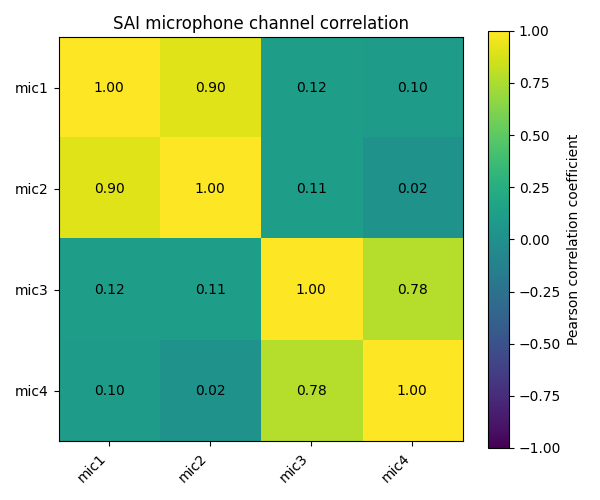
\includegraphics[width=\textwidth]{Figures/sai_correlation_matrix.png}
        \caption[Signal correlation for the SAI]{Signal correlation matrix between each microphone pair using the SAI}
        \label{fig:corr_sai}
    \end{subfigure}
    \hfill
    \begin{subfigure}[b]{0.48\textwidth}
        \centering
        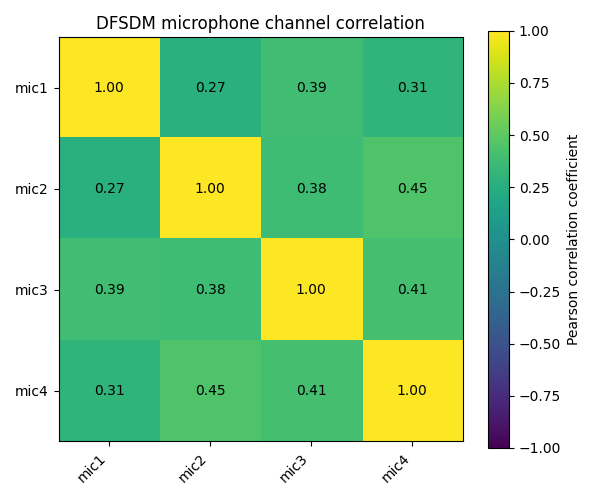
\includegraphics[width=\textwidth]{Figures/dfsdm_correlation_matrix.png}
        \caption[Signal correlation for the DFSDM]{Signal correlation matrix between each microphone pair using the DFSDM}
        \label{fig:corr_dfsdm}
    \end{subfigure}
    \caption{Comparison between the microphone pair correlations using SAI and DFSDM for sound acquisition}
\label{fig:corr_comparison}
\end{figure}

\newpage
    \subsection{DC offset removal}
    The results of the DC offset removal can be seen in Figure~\ref{fig:dc_offset_dfsdm}. As expected, the values were centered around zero.

    \begin{figure}[h]
        \centering
        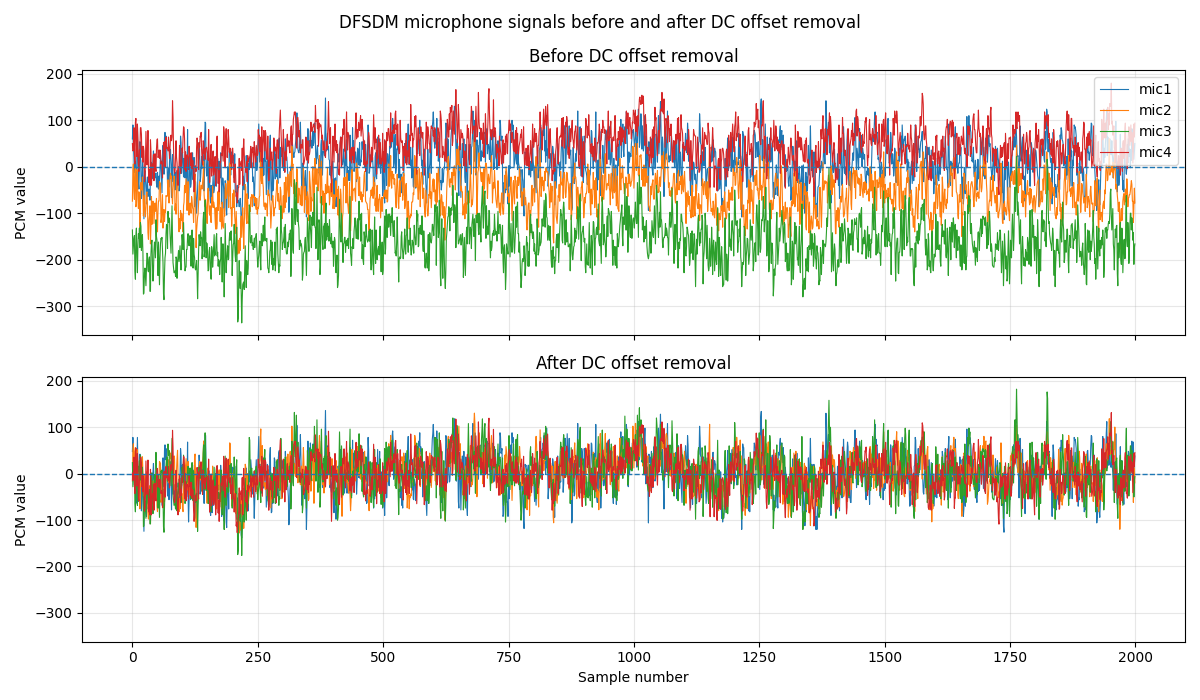
\includegraphics[width=0.65\linewidth]{Figures/DC_offset for dfsdm.png}
        \caption{Results of the DC offset for the microphone signal}
        \label{fig:dc_offset_dfsdm}
    \end{figure}
    
\section{DOA estimation testing results}
The DOA estimation results are presented in three stages: human-generated sounds, recorded drone-like sounds, and live-drone testing.

\subsection{Results of the first DOA testing stage}
In the empty classroom, the DOA estimate pointed close to the expected source direction when the student was positioned at approximately 90 degrees, as shown in Figure~\ref{fig:DOA_estimation_first_stage}.

\begin{figure}[h]
    \centering
    %\begin{subfigure}[b]{0.48\linewidth}
    %    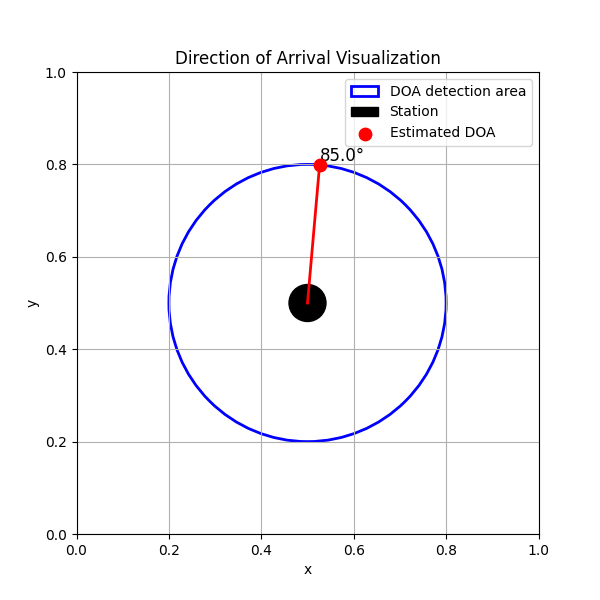
\includegraphics[width=\linewidth]{Figures/Debug_doa_estimation1777722708.9166152.png}
    %    \caption{First stage estimation nr.1 (empty classroom)}
    %    \label{fig:f_stage_est_1}
    %\end{subfigure}
    %\hfill
    %\begin{subfigure}[b]{0.48\linewidth}
    %    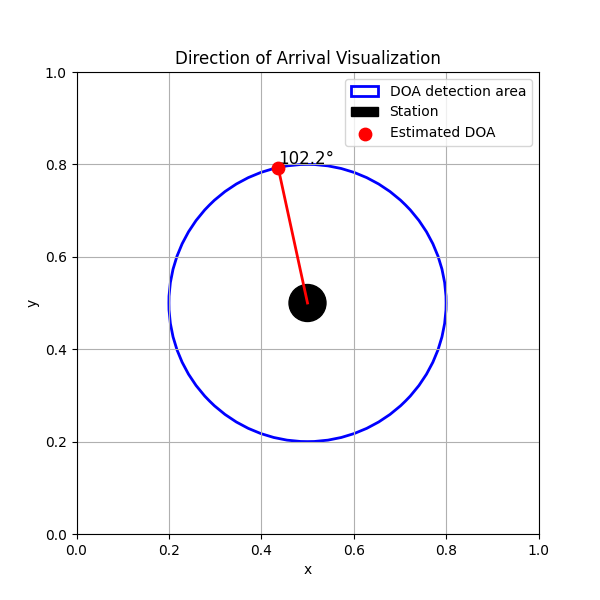
\includegraphics[width=\linewidth]{Figures/Debug_doa_estimation1777722714.2824512.png}
    %    \caption{First stage estimation nr.2 (empty classroom)}
    %    \label{fig:f_stage_est_1}
    %\end{subfigure}
    %\hfill
    \begin{subfigure}[b]{0.3\linewidth}
        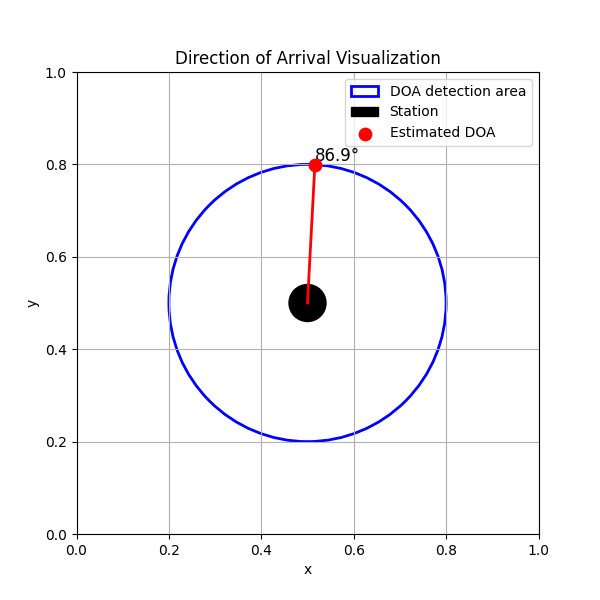
\includegraphics[width=\linewidth]{Figures/Debug_doa_estimation1777722716.9580076.png}
        \caption{First stage estimation nr.3 (empty classroom)}
        \label{fig:f_stage_est_1}
    \end{subfigure}
    \hfill
    \begin{subfigure}[b]{0.3\linewidth}
        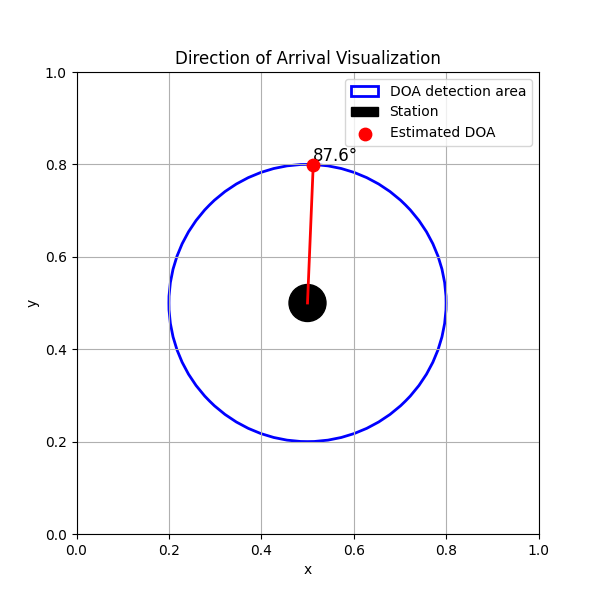
\includegraphics[width=\linewidth]{Figures/Debug_doa_estimation1777722719.6664054.png}
        \caption{First stage estimation nr.4 (empty classroom)}
        \label{fig:f_stage_est_1_2}
    \end{subfigure}
    \hfill
    \caption{DOA estimation for the first testing stage, with an empty calssroom}
    \label{fig:DOA_estimation_first_stage}
\end{figure}
\newpage

However in the occupied classroom, the results changed significantly. The DOA estimate no longer pointed consistently towards the intended test sound. Instead, the estimated direction was often towards a group of students talking in the room at angle of approximately 45 degrees from the system, as seen in Figure~\ref{fig:DOA_estimation_first_stage_full_class}. This proves that the DOA module estimated the direction of the dominant sound source rather than the desired test sound source. 

\begin{figure}[h]
    \centering
    \begin{subfigure}[b]{0.48\linewidth}
        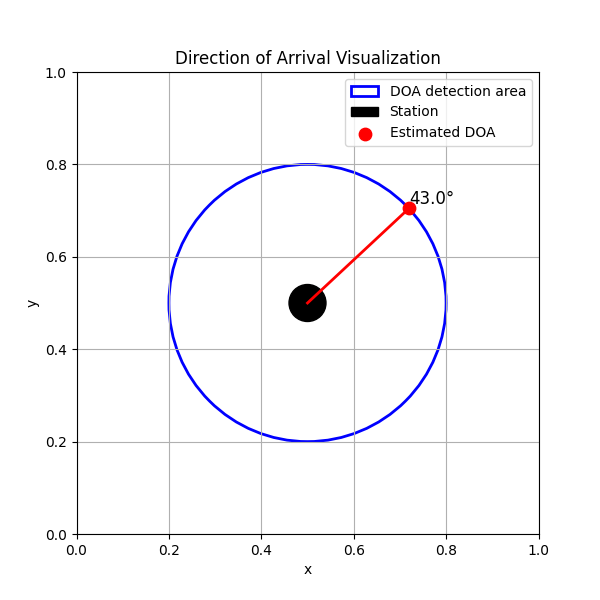
\includegraphics[width=\linewidth]{Figures/Debug_doa_estimation1777723161.8334353.png}
        \caption{First stage estimation nr.1 (full classroom)}
        \label{fig:f_stage_est_1_f}
    \end{subfigure}
    \hfill
    \begin{subfigure}[b]{0.48\linewidth}
        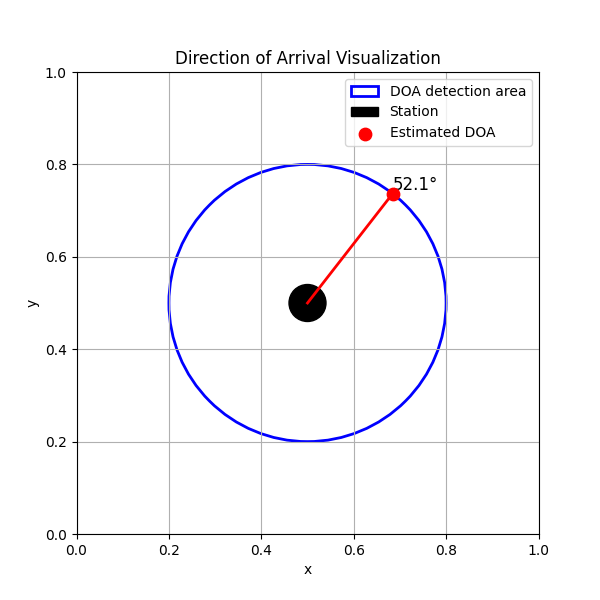
\includegraphics[width=\linewidth]{Figures/Debug_doa_estimation1777723163.390828- VIKTIG 2.png}
        \caption{First stage estimation nr.2 (full classroom)}
        \label{fig:f_stage_est_2_f}
    \end{subfigure}
   % \hfill
   % \begin{subfigure}[b]{0.48\linewidth}
   %     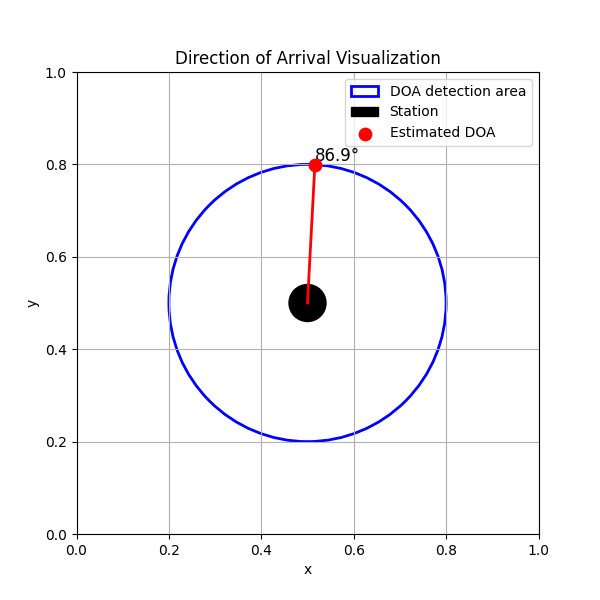
\includegraphics[width=\linewidth]{Figures/Debug_doa_estimation1777722716.9580076.png}
   %     \caption{First stage estimation nr.3 (full classroom)}
   %     \label{fig:f_stage_est_3_f}
   % \end{subfigure}
   % \hfill
   % \begin{subfigure}[b]{0.48\linewidth}
    %    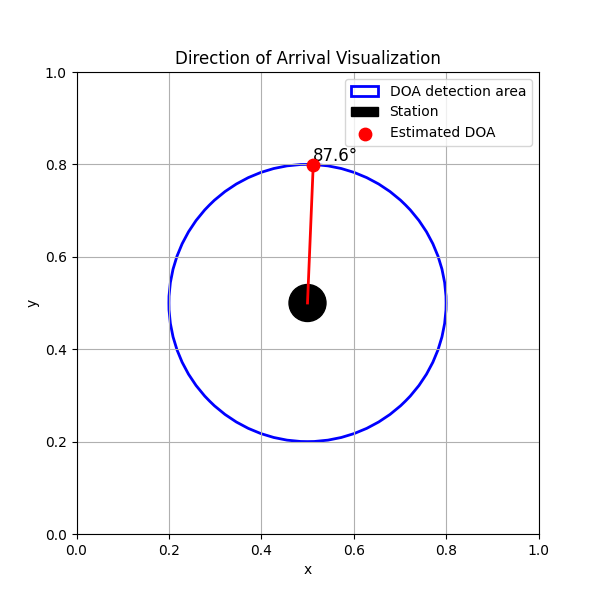
\includegraphics[width=\linewidth]{Figures/Debug_doa_estimation1777722719.6664054.png}
   %     \caption{First stage estimation nr.4 (full classroom)}
   %     \label{fig:f_stage_est_4_f}
   % \end{subfigure}
    \hfill
    \caption{DOA estimation for the first testing stage, with a full calssroom}
    \label{fig:DOA_estimation_first_stage_full_class}
\end{figure}

These results supported the need for a classification stage before the DOA result is interpreted as a drone direction. Without such classification, the DOA module may estimate the direction of other dominant sounds in the environment. 
\newpage
\subsection{The second DOA testing stage}
The DC motor test did not produce reliable DOA estimates at distances above a few centimeters. The system was unable to detect the DC-motor, which resulted in random DOA estimation. When the DC-motor was being hold around 30 cm away from the microphone platform, the DOA estimation was as accurate as for the human sound on the distance of few meters. The frequency bands present in the signal, can be seen in Figure~\ref{fig:dc_motor_mel}. 

\begin{figure}[h]
    \centering
    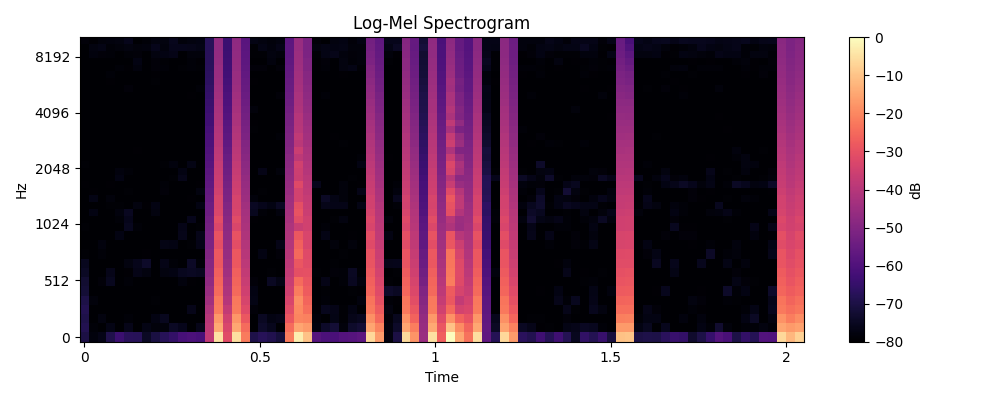
\includegraphics[width=0.5\linewidth]{Figures/Debug_mel_spectrogram1777801048.636684.png}
    \caption[DC-motor Mel-spectrogram]{The components present in the acoustic signal produced by the DC-motor}
    \label{fig:dc_motor_mel}
\end{figure}

The next test, was conducted by using the drone sound from the video, which resulted in a consistent and accurate DOA estimation on the testing distance, as can be seen in Figure~\ref{fig:DOA_estimation_second_stage}. The frequency bands present in the signal are shown in Figure~\ref{fig:mel_specs}.       

\begin{figure}[h]
    \centering
    \begin{subfigure}[b]{0.4\linewidth}
        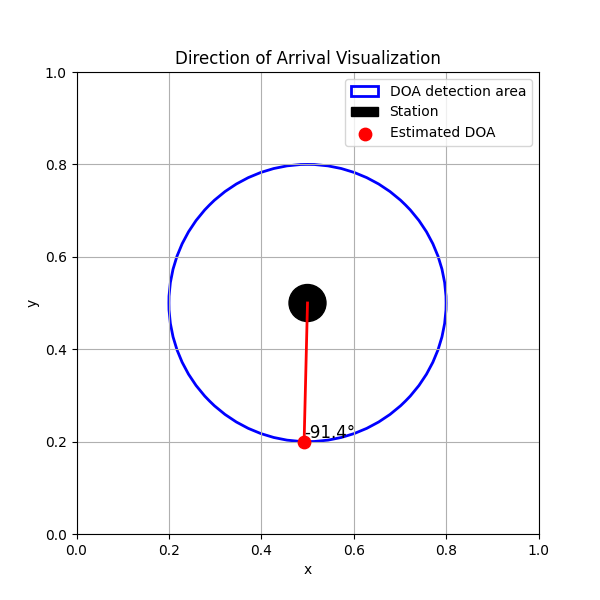
\includegraphics[width=\linewidth]{Figures/Debug_doa_estimation1777801847.8342373.png}
        \caption{Second stage estimation nr.1}
        \label{fig:f_stage_est_1_f}
    \end{subfigure}
    \hfill
    \begin{subfigure}[b]{0.4\linewidth}
        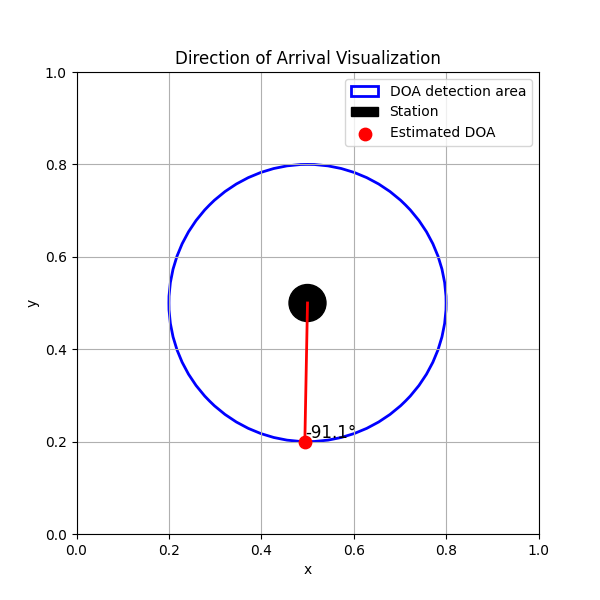
\includegraphics[width=\linewidth]{Figures/Debug_doa_estimation1777801851.314917.png}
        \caption{Second stage estimation nr.2}
        \label{fig:f_stage_est_2_f}
    \end{subfigure}
    \hfill
    \caption{DOA estimation for the second testing stage using the drone video}
    \label{fig:DOA_estimation_second_stage}
\end{figure}
\newpage
\begin{figure}[h]
    \centering
    \begin{subfigure}[b]{0.4\linewidth}
        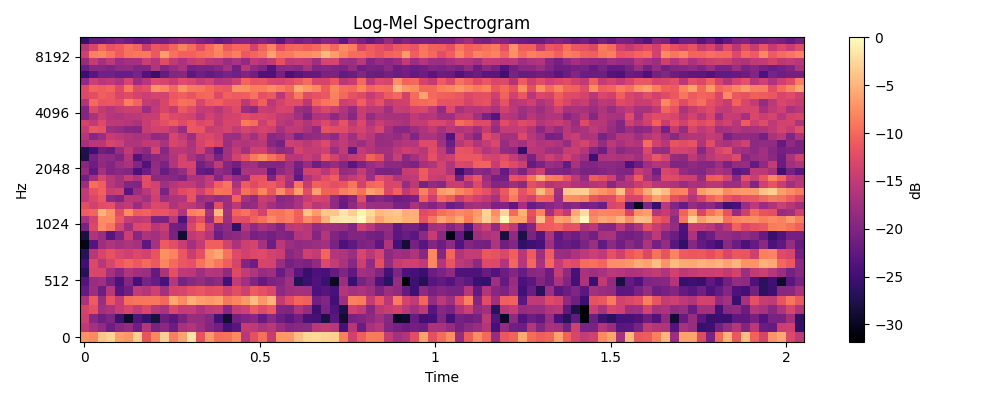
\includegraphics[width=\linewidth]{Figures/Debug_mel_spectrogram1777801847.8342373.png}
        \caption{Mel-spectrogram from the second stage DOA testing nr.1}
        \label{fig:mel_spec_1}
    \end{subfigure}
    \hfill
    \begin{subfigure}[b]{0.4\linewidth}
        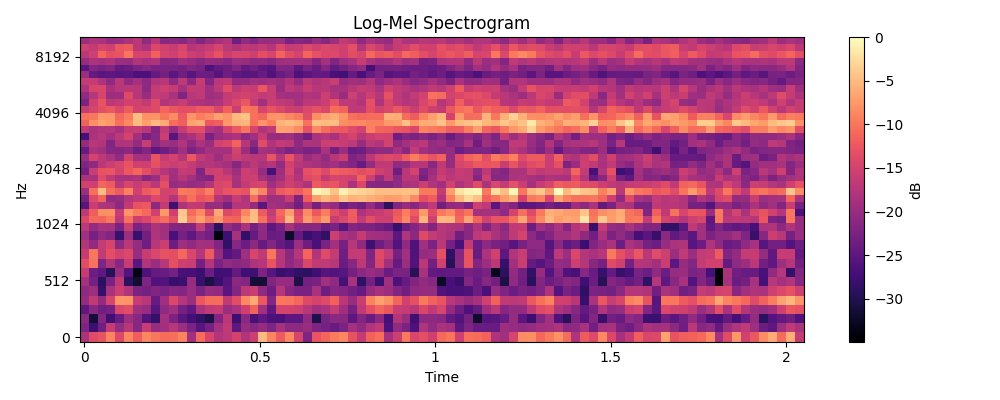
\includegraphics[width=\linewidth]{Figures/Debug_mel_spectrogram1777801851.314917.png}
        \caption{Mel-spectrogram from the second stage DOA testing nr.2}
        \label{fig:mel_spec_2}
    \end{subfigure}
    \hfill
    \caption{Mel-spectrograms produced during the second stage of DOA testing}
    \label{fig:mel_specs}
\end{figure}

The results of the test invloving the sound volume of around 50\% were mixed, as the drone signal was for the most part not recorded by the system, which resulted in less reliable DOA estimation.\\

The last test where the sound was reduced to around 5\% resulted in complete lack of drone detection, which resulted in random DOA estimation.\\

Since the drone sound was for the most part not detected, when using the phone volume of 50\% and 5\%, the received signals were compared by calculating the RMS values across the microphone channels after the DC offset removal. The 100\% phone volume test, had the highest received PCM level, while the 50\% and 5\% volume tests were approximately 9db lower as seen in Figure~\ref{fig:rms_phone_volumes}. However the 50\% and 5\% tests have produced quite similair RMS values, which may indicate that both signals were strongly influenced by the background noise. 

\begin{figure}[h]
    \centering
    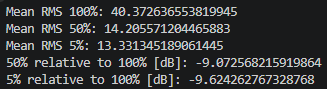
\includegraphics[width=0.5\linewidth]{Figures/image.png}
    \caption{The RMS values for the drone sound produced by the phone of varying volume levels}
    \label{fig:rms_phone_volumes}
\end{figure}

The second stage of the DOA testing, has proven that the system is capable of detecting the drone, if the sound produced by it is loud enough.\\

\subsection{The third DOA testing stage}
The result of the first no drone present test, conducted to measure the noise level in the laboratory was saved as the  Mel-spectrogram is shown in Figure~\ref{fig:stage_3_noise_present_no_drone}. Since the ML classification was not applied during the baseline test, the DOA module could still estimate the sound direction based on the dominant background noise, which proved again, that the ML has to be applied for the system to correctly estimate the DOA of the incoming drone.\\

\begin{figure}[h]
    \centering
    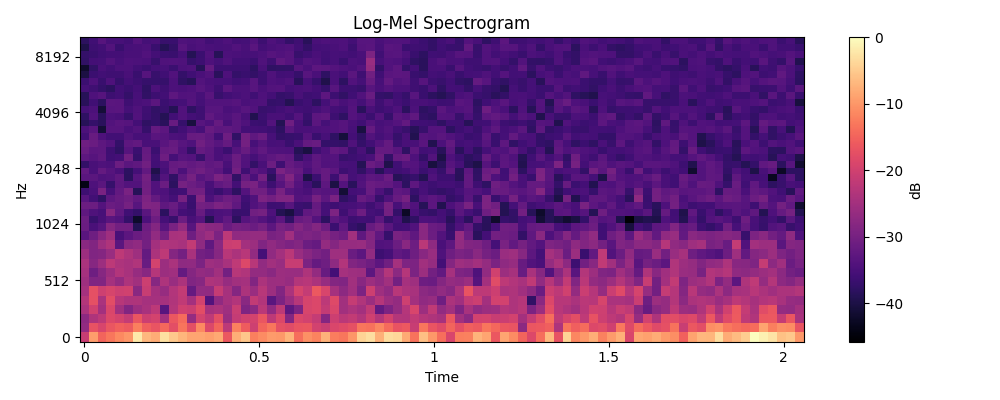
\includegraphics[width=0.5\linewidth]{Figures/Debug_mel_spectrogram1777882767.382446.png}
    \caption{Noisy frequency bands}
    \label{fig:stage_3_noise_present_no_drone}
\end{figure}
\newpage

The next test involving the use of the live-drone, which was circulating around the tower has resulted in the DOA estimation seen in Figure~\ref{fig:3_stage_no_camera-doa} and the following Mel-spectrogram seen in Figure~\ref{fig:mel_spec_present}. The resulting DOA estimation was quite accuarate, and the final test involving the ML and camera could be conducted.  \\

\begin{figure}[h]
    \centering
    \begin{subfigure}[b]{0.5\linewidth}
        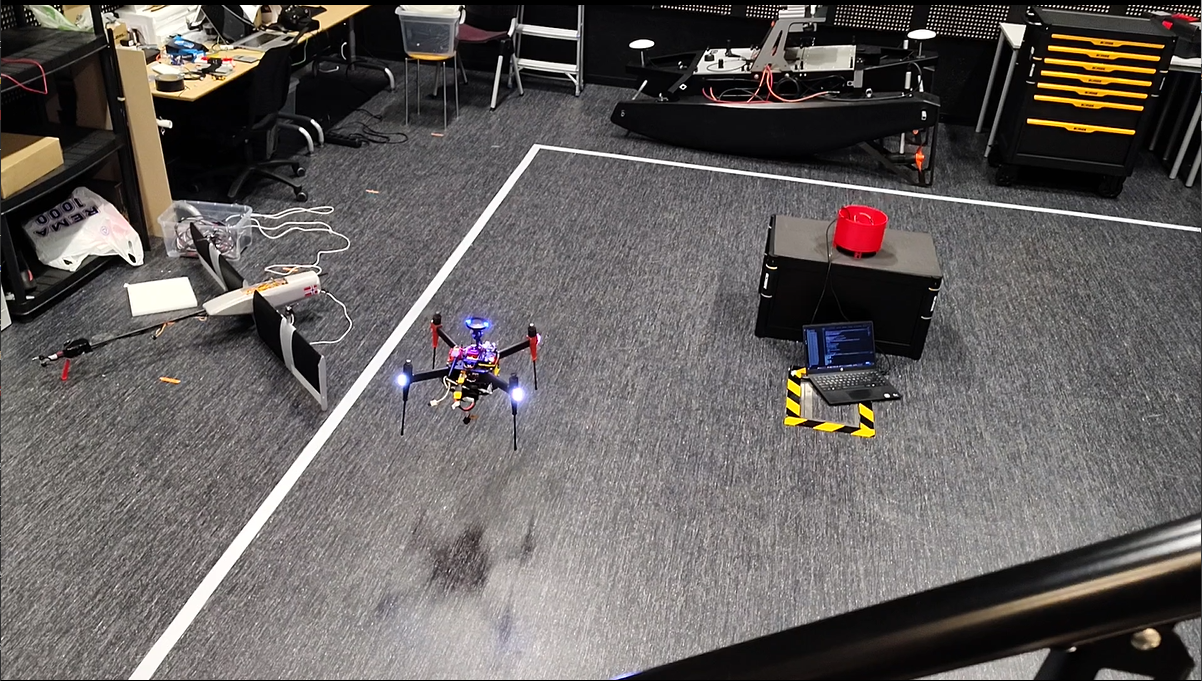
\includegraphics[width=\linewidth]{Figures/test_doa_no_camera.png}
    \caption{The actual drone position}
    \label{fig:picture_drone_position}
    \end{subfigure}
    \hfill
    %\vspace{2em}
    \begin{subfigure}[b]{0.40\linewidth}
        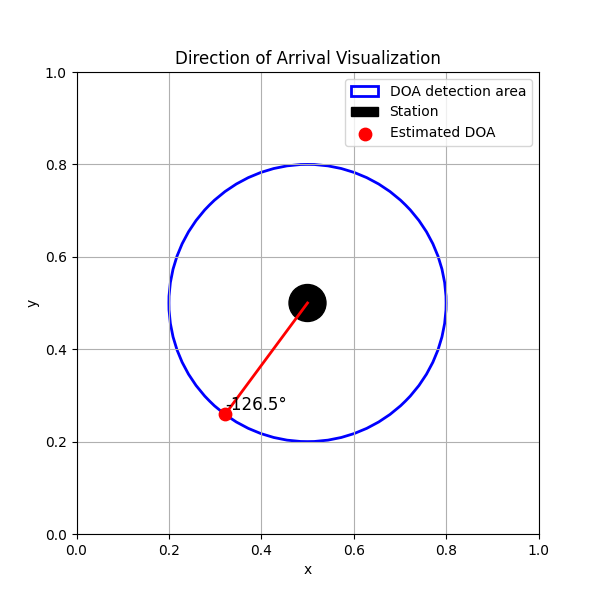
\includegraphics[width=\linewidth]{Figures/Debug_doa_estimation1777884326.4922612.png}
    \caption{The estimated DOA of the drone present}
    \label{fig:doa_estimation_3_stage_no_camera}
    \end{subfigure}
    \hfill
    \begin{subfigure}[b]{0.5\linewidth}
        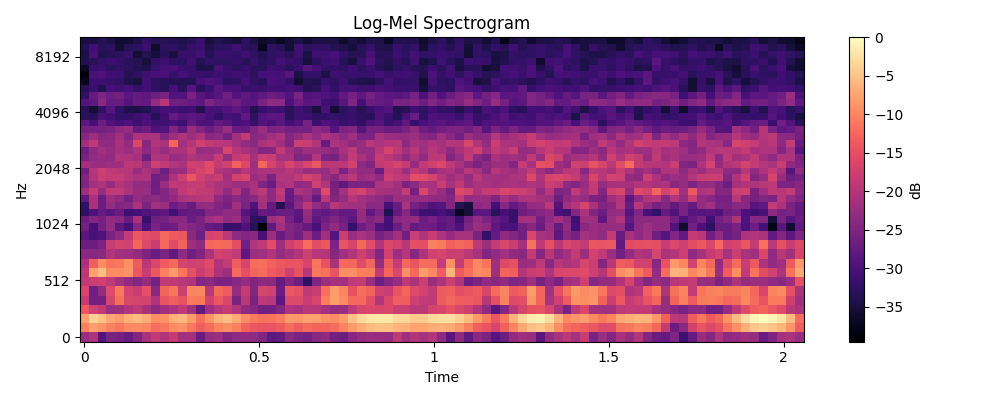
\includegraphics[width=1\linewidth]{Figures/Debug_mel_spectrogram1777884268.2983675.png}
    \caption{Mel-spectrogram for the drone present}
    \label{fig:mel_spec_present}
    \end{subfigure}
    \hfill
    \caption{The first DOA estimation using the live-drone, without the ML or the camera}
    \label{fig:3_stage_no_camera-doa}
\end{figure}
  

The results of the final DOA test, where ML and camera was implemented, can be seen in Figure~\ref{fig:doa_screenshots}.\\

\begin{figure}[H]
    \centering
    \begin{subfigure}[b]{0.48\linewidth}
        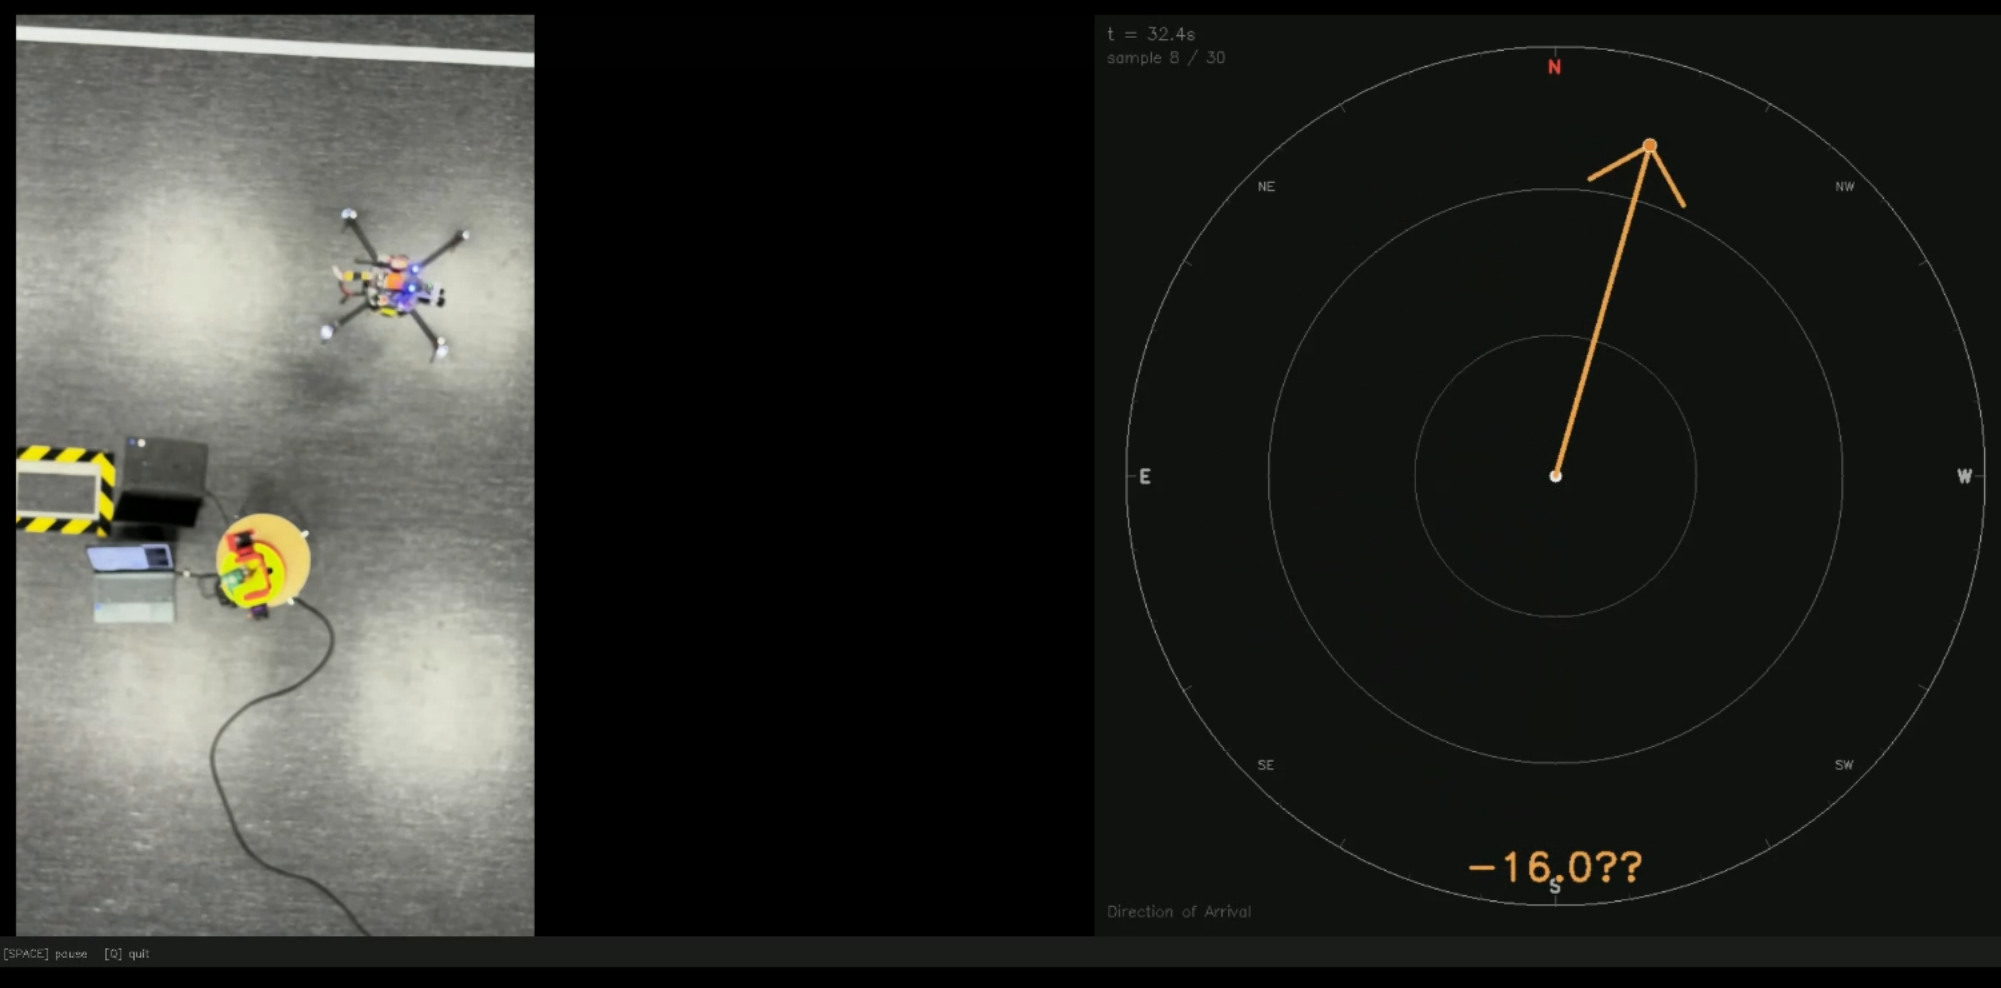
\includegraphics[width=\linewidth]{Figures/Andreas/DOA_estimation/Drone_DOA_1.png}
        \caption{}
        \label{fig:doa1}
    \end{subfigure}
    \hfill
    \begin{subfigure}[b]{0.48\linewidth}
        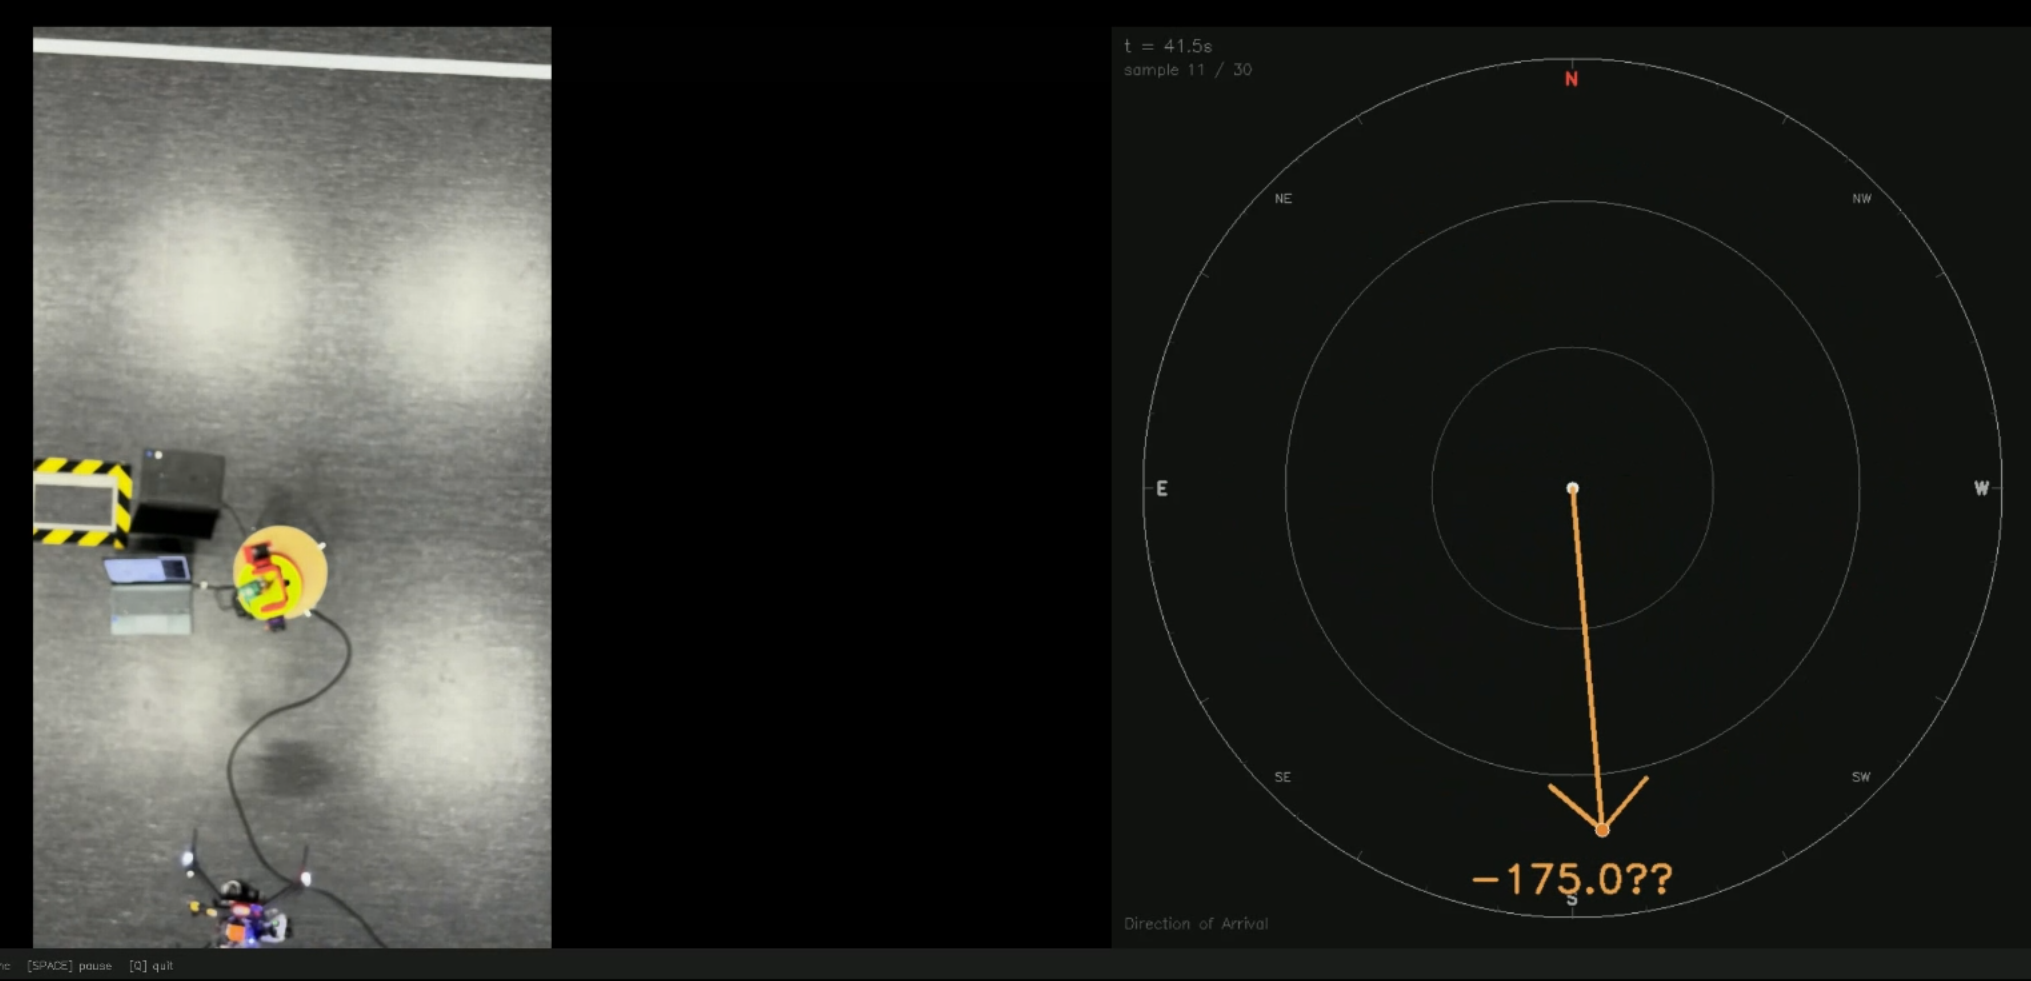
\includegraphics[width=\linewidth]{Figures/Andreas/DOA_estimation/Drone_DOA_2.png}
        \caption{}
        \label{fig:doa2}
    \end{subfigure}

    \vspace{0.5em}

    \begin{subfigure}[b]{0.48\linewidth}
        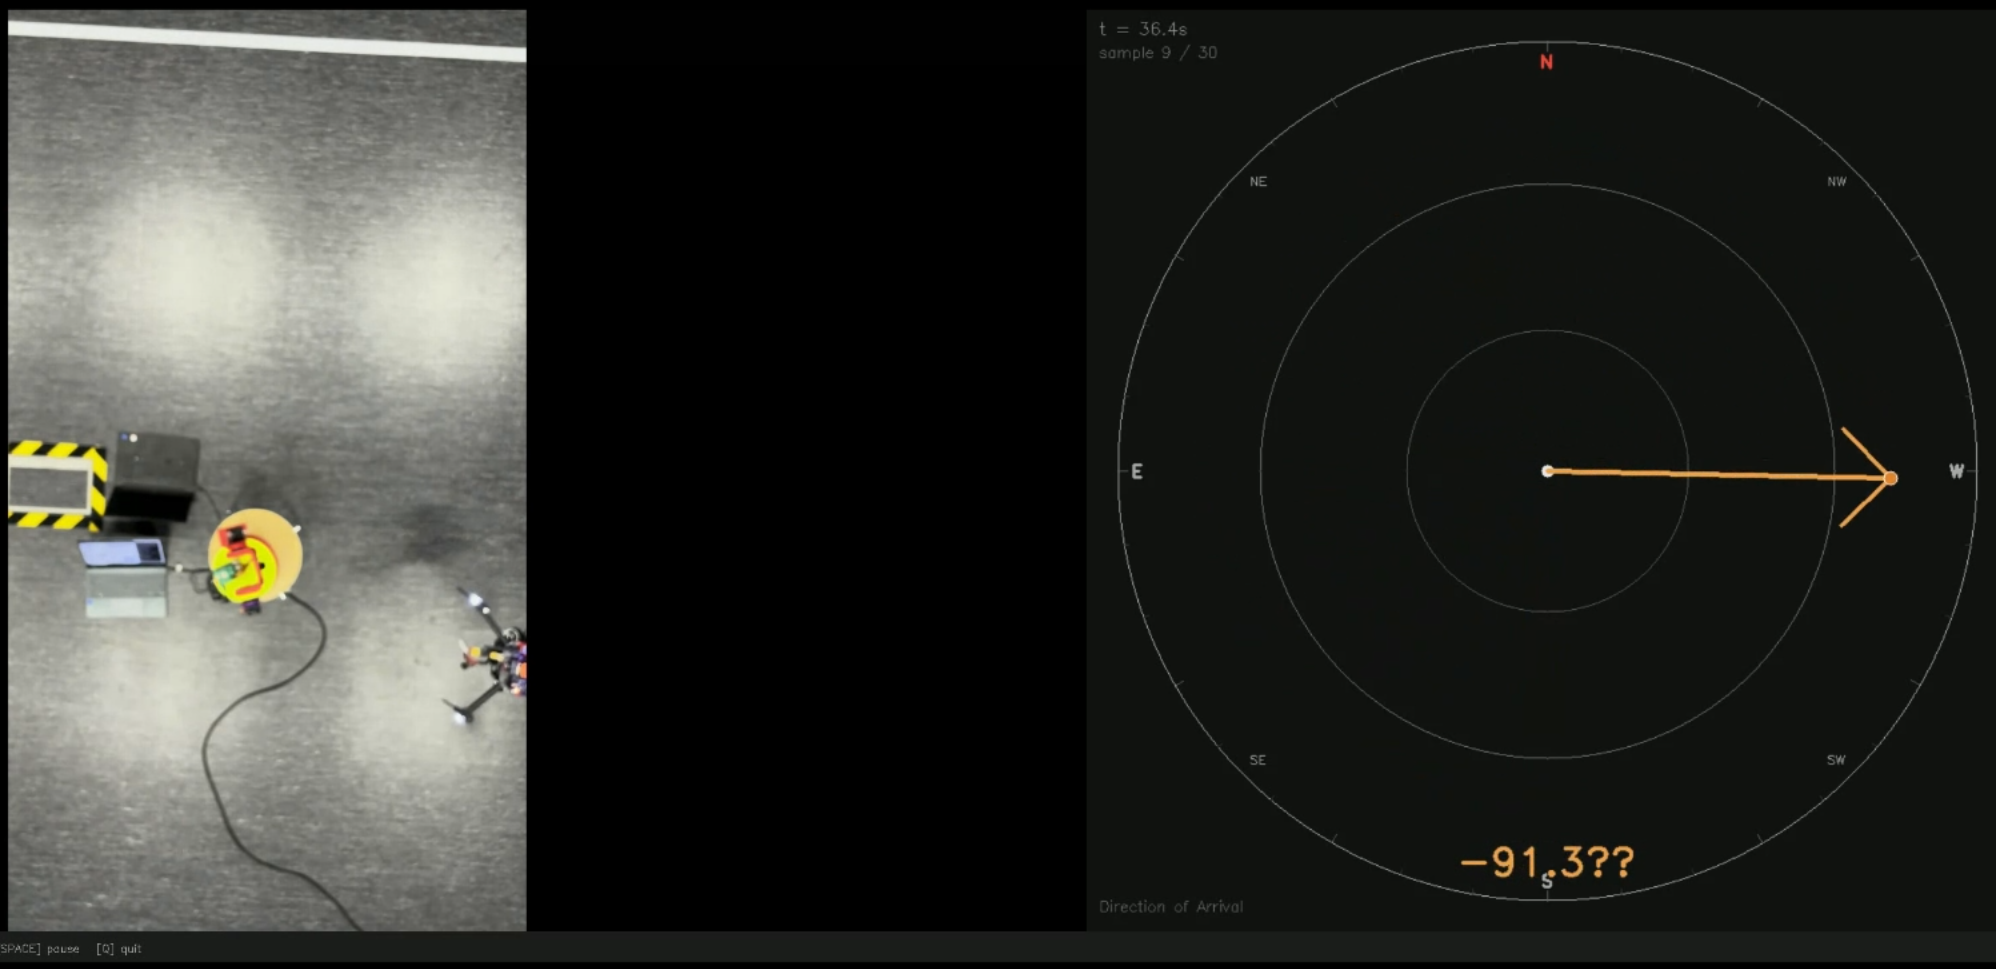
\includegraphics[width=\linewidth]{Figures/Andreas/DOA_estimation/Drone_DOA_3.png}
        \caption{}
        \label{fig:doa3}
    \end{subfigure}
    \hfill
    \begin{subfigure}[b]{0.48\linewidth}
        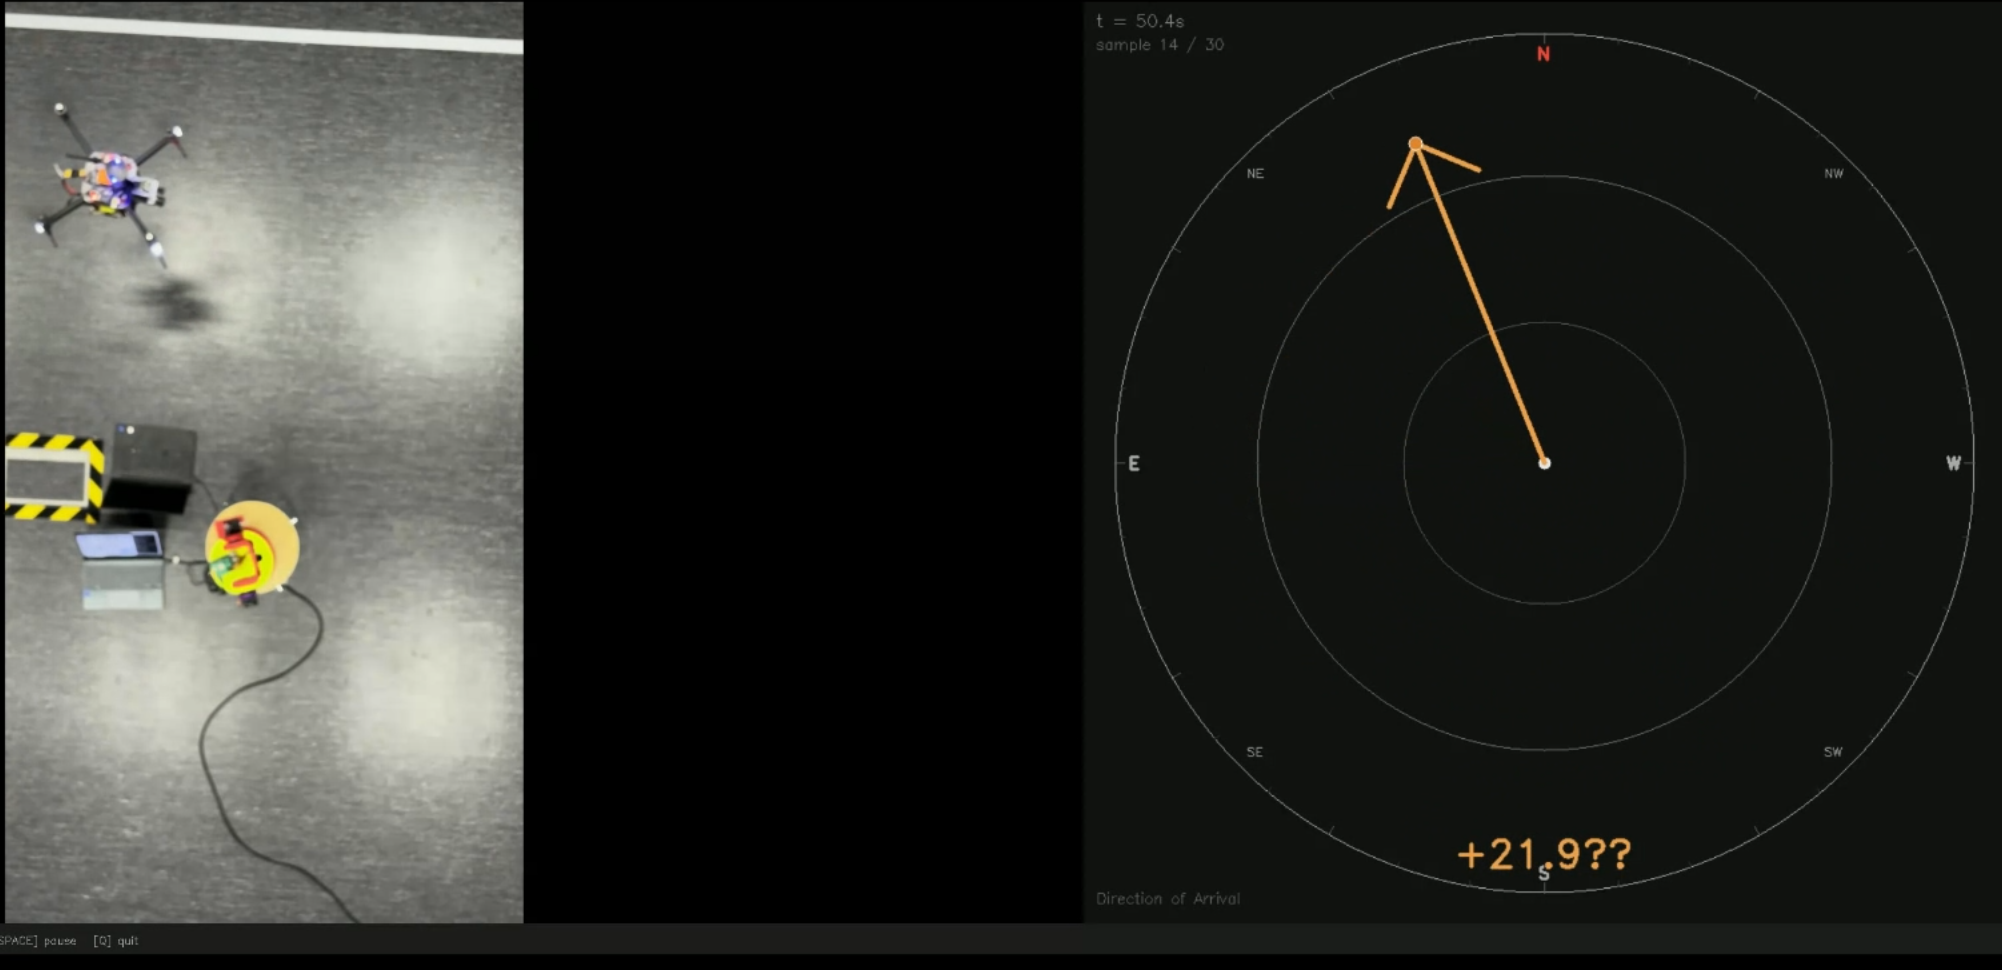
\includegraphics[width=\linewidth]{Figures/Andreas/DOA_estimation/Drone_DOA_4.png}
        \caption{}
        \label{fig:doa4}
    \end{subfigure}

    \caption{DOA estimation of the drone circulating around the tower.}
    \label{fig:doa_screenshots}
\end{figure}

The results of the Ml classification and the DOA estimation were consistent and accurate. However, it turned out during the testing process, that the lag produced by the system was more significant then expected as seen in Figure~\ref{fig:time_between_each_iteration}. The second DOA estimate was produced after around 9 seconds after the first estimation, which might be caused by the system startup. The other consecutive estimations were generated in 3.24 seconds on average. The main reason for doubling of the expected time needed for DOA estimation, might be the generation of the DOA visualization and Mel-spectrogram figures used for debuging.    

\begin{figure}[h]
    \centering
    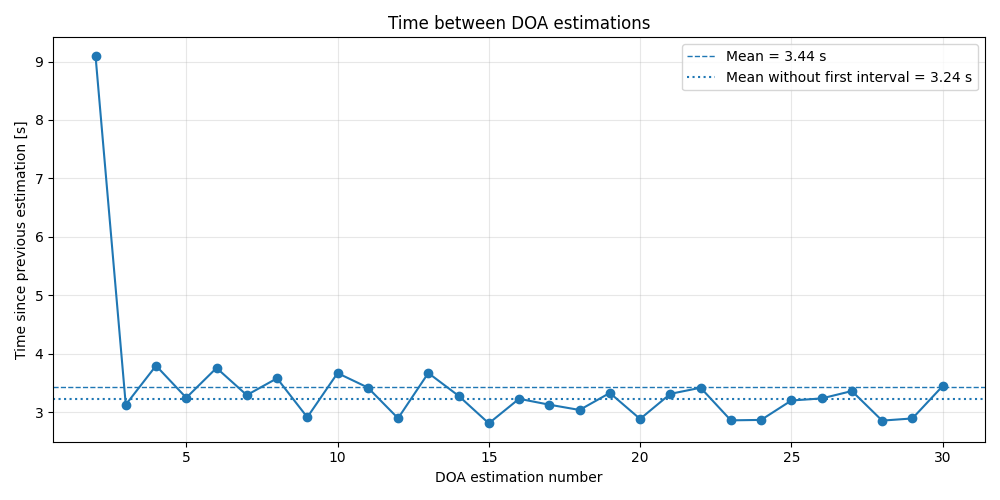
\includegraphics[width=0.5\linewidth]{Figures/time_between_each_estimation.png}
    \caption{Time between each iteration produced during the final test}
    \label{fig:time_between_each_iteration}
\end{figure}

The system lag, was later tested without the figure generation modules, which resulted in Figure~\ref{fig:time_lag_no_figure}, which shows that the lag time was indeed caused by the figure generation. The test was also conducted without the ML, which is expected to produce approx.25 ms of lag per iteration and around 250 ms during the initialization period, as seen in Figure~\ref{fig:ml_time}.

\begin{figure}[h]
    \centering
    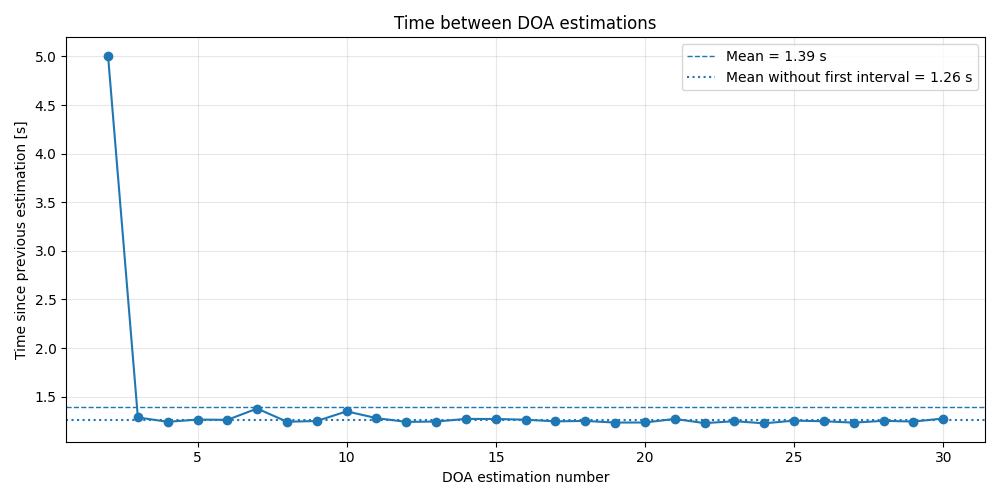
\includegraphics[width=0.5\linewidth]{Figures/time_test_without_figure_production_no_ML.png}
    \caption{Time between each iteration produced without the figure generation methods}
    \label{fig:time_lag_no_figure}
\end{figure}

\begin{figure}[h]
    \centering
    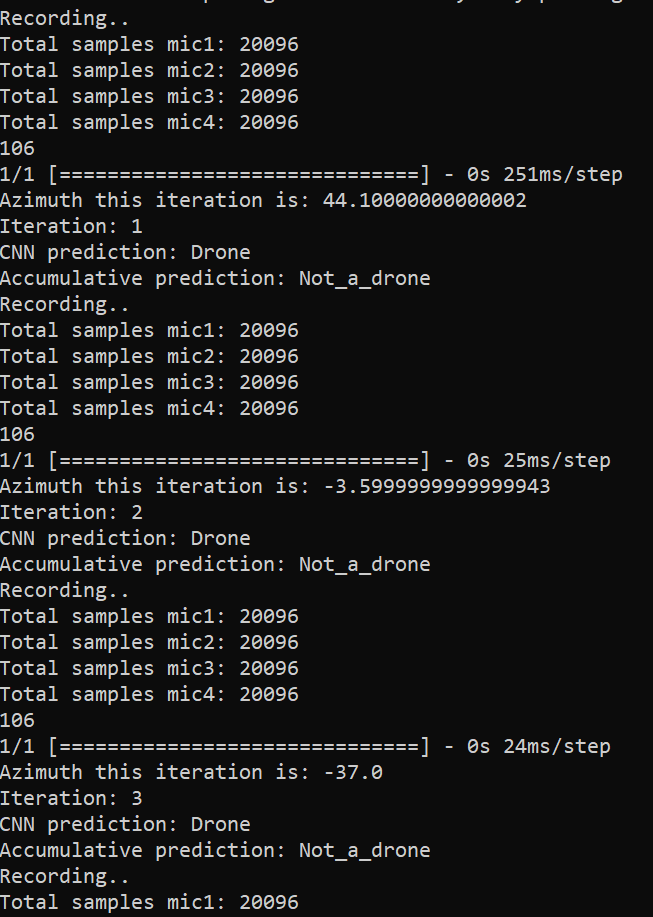
\includegraphics[width=0.3\linewidth]{Figures/times ml.png}
    \caption{Time duration needed for ML classification}
    \label{fig:ml_time}
\end{figure}

So by adding the time needed for ML to classify the sound source, the total time needed for one iteration is around 1.285 s.  

\newpage

\section{MFCC extraction}

    \subsection{Spectrogram and Mel-spectrogram representation}
    In the early stages of the signal acquisition testing, both the spectrograms and the Mel-spectrograms were generated to visualize the frequency bands present in the acquired signal. As seen in Figure~\ref{fig:spectrograms}, the Mel-spectrogram is able to represent the available frequency bands with more detail then the "normal" spectrogram. 
    
    \begin{figure}[H]
    \centering
    \begin{subfigure}[b]{0.48\textwidth}
        \centering
        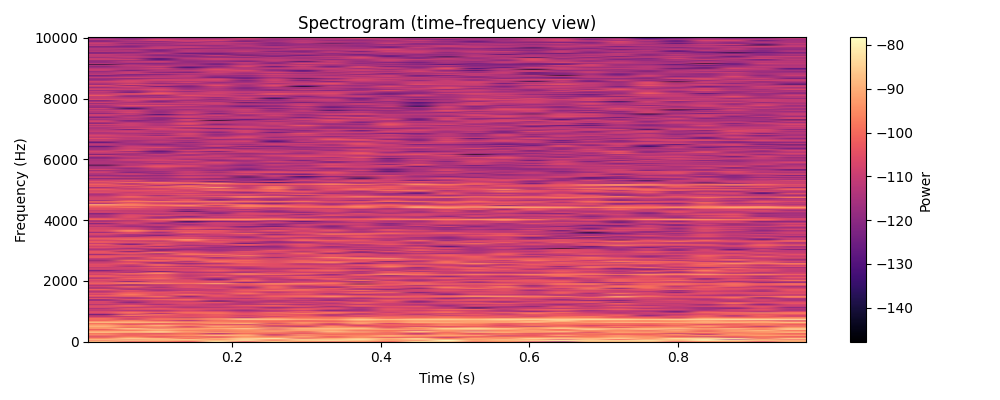
\includegraphics[width=\textwidth]{Figures/Debug_spectrogram1777884217.5826006.png}
        \caption{Spectrogram}
        \label{fig:spectrogram}
    \end{subfigure}
    \hfill
    \begin{subfigure}[b]{0.48\textwidth}
        \centering
        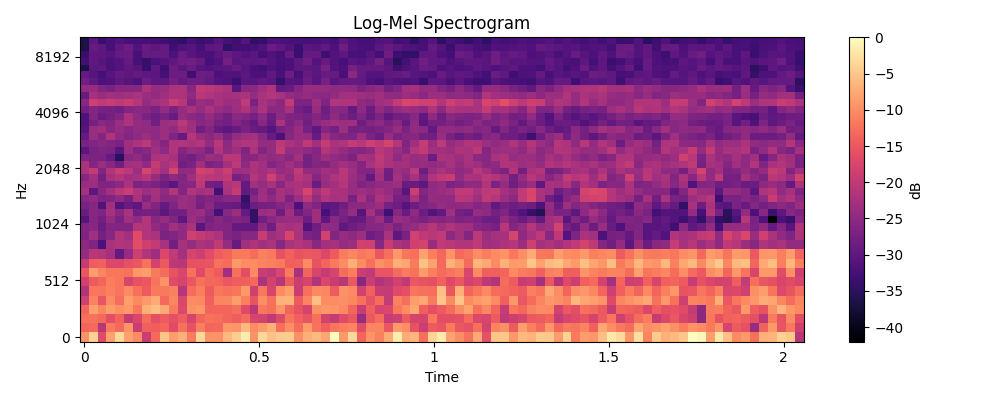
\includegraphics[width=\textwidth]{Figures/Debug_mel_spectrogram1777884217.5826006.png}
        \caption{Mel-spectrogram}
        \label{fig:mel_spectrogram}
    \end{subfigure}
    \caption{Spectrogram types generated during the testing process}
\label{fig:spectrograms}
\end{figure}

   \subsection{Mel-spectrograms from DOA testing}
    During the testing process, the system has produced different Mel-spectrograms, where each was representing unique frequency bands present in the signal. 
    
        \subsubsection{First stage: human-generated sounds}

        The behaviour of the signal representing the calpping sound can be seen in Figure~\ref{fig:clapping_mel_spec}. During the recording period, the student clapped three times, which produced three short high-energy regions in the Mel-spectrogram. The clapping sound excited a broad range of recorded frequency bands, while the strongest visible energy appears to be concentrated around approximately 3000 Hz. 

        \begin{figure}[h]
            \centering
            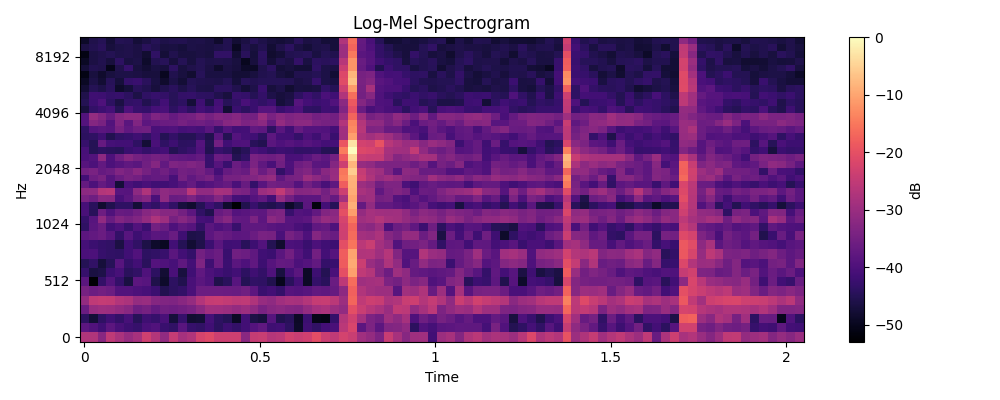
\includegraphics[width=0.75\linewidth]{Figures/Debug_mel_spectrogram1777802028.6846912.png}
            \caption{Mel-spectrogram representing the clapping sound produced during the first testing stage.}
            \label{fig:clapping_mel_spec}
        \end{figure}
\newpage
        \subsubsection{Second stage: drone-like and recorded drone sounds}

        The behaviour of the DC-motor signal. which was meant to imitate the drone sound can be seen in Figure~\ref{fig:mel_spec_dc_motor}. The signal produced several short high-energy regions, mostly concentrated around the lower frequency bands. The DC-sound compared to the clapping sound, seamed to be less consistent over time, and wasn't at all hearable by the system at the distance greater then 30 cm.

        \begin{figure}[h]
            \centering
            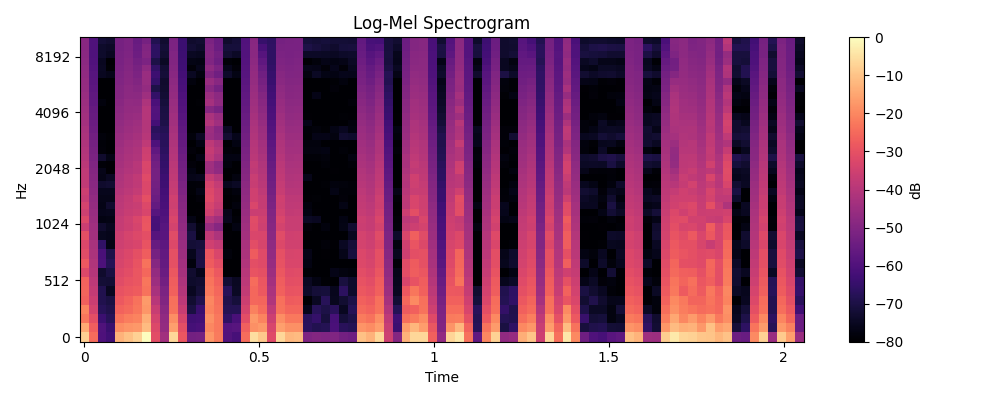
\includegraphics[width=0.75\linewidth]{Figures/Debug_mel_spectrogram1777725034.3948312.png}
            \caption{Mel-spectrogram representing the sound produced by the DC-motor}
            \label{fig:mel_spec_dc_motor}
        \end{figure}
\newpage
        The drone sound produced by the youtube video can be seen in Figure~\ref{fig:mel_spec_youtube}. Compared with the DC-motor signal, the recorded drone sound produced more continuous and stable frequency components over time. Several horizontal bands are visible in the Mel-spectrogram, especially in the lower and middle frequency range. This indicates, that the drone recording contained some harmonic components, which allowed for accurate and consistent DOA estimation of the sound source, when the phone volume was set to maximum. 

        \begin{figure}[h]
            \centering
            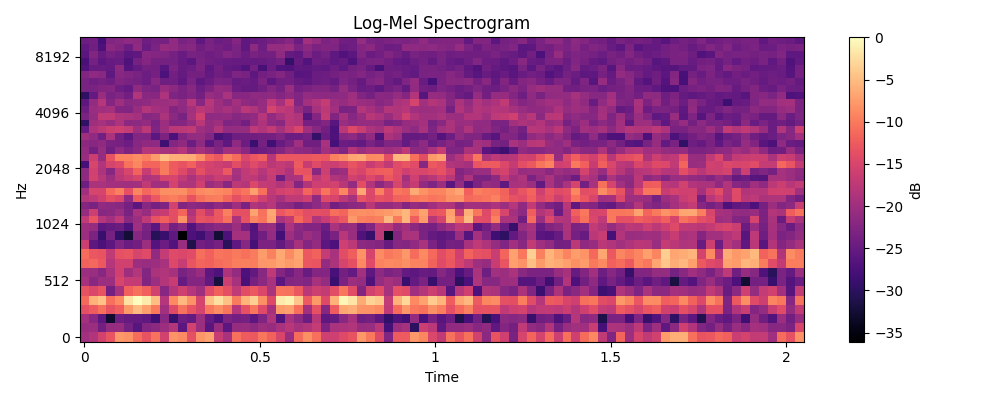
\includegraphics[width=0.75\linewidth]{Figures/Debug_mel_spectrogram1777804261.3530798.png}
            \caption{Mel-spectrogram representing the drone sound produced by the youtube video}
            \label{fig:mel_spec_youtube}
        \end{figure}
        
        \subsubsection{Third stage: live drone sound}

        The sound produced by the live drone showed similar horizontal bands to the drone sound played from the video, especially in the lower frequency range. However, the live-drone spectrogram appeared to contain less high-frequency content, as seen in Figure~\ref{fig:mel_spec_live_drone}. This difference may be related to the different test conditions. The live-drone test was conducted in the laboratory, where room reflections, background noise, and the shorter distance between the drone and the tower may have affected the recorded frequency content. In addition, the live drone produced a significantly louder acoustic signal than the phone playback, which likely made the lower-frequency drone components more dominant in the recording.

        \begin{figure}[h]
            \centering
            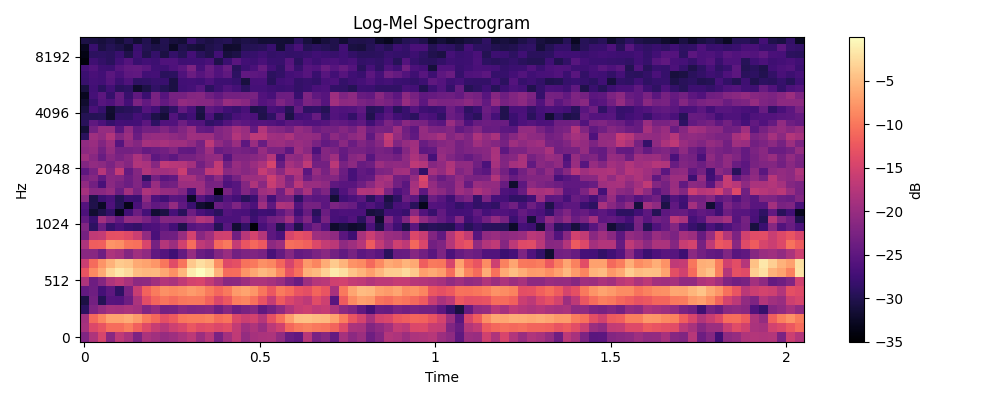
\includegraphics[width=0.75\linewidth]{Figures/Debug_mel_spectrogram1778753123.3731422.png}
            \caption{Mel-spectrogram representing the sound produced by the live-drone}
            \label{fig:mel_spec_live_drone}
        \end{figure}
        \newpage

        The Mel-spectrograms used during the system testing showed clear differnces between the tested sound sources. The clapping sound produced short boradband energy source, while the sound produced by drone, either from the youtube video, or the live-drone, produced the continous horizontal frequency bands. The visual comparison between the signals, has also shown how big of an influnece the testing enviroment can have on the noise present in the deteced signal. Therefore, the Mel-spectrograms privided useful support for system testing and training of the ML algorithm. 
          
    %mention the need of redesigning the pcb, to use another motor drive

\section{YOLO Hardware test}
The average intereference time with the HAILO chip was found to be 9.2ms whereas with CPU only it was 235.6ms. (\ref{fig:Interference_comp}) The Raspberry PI 5 was therefore found to be able to run the YOLO detection model at around 108 intereferences pr second, whereas for CPU only it was around 3.75. 

\begin{figure}[H]
    \centering
    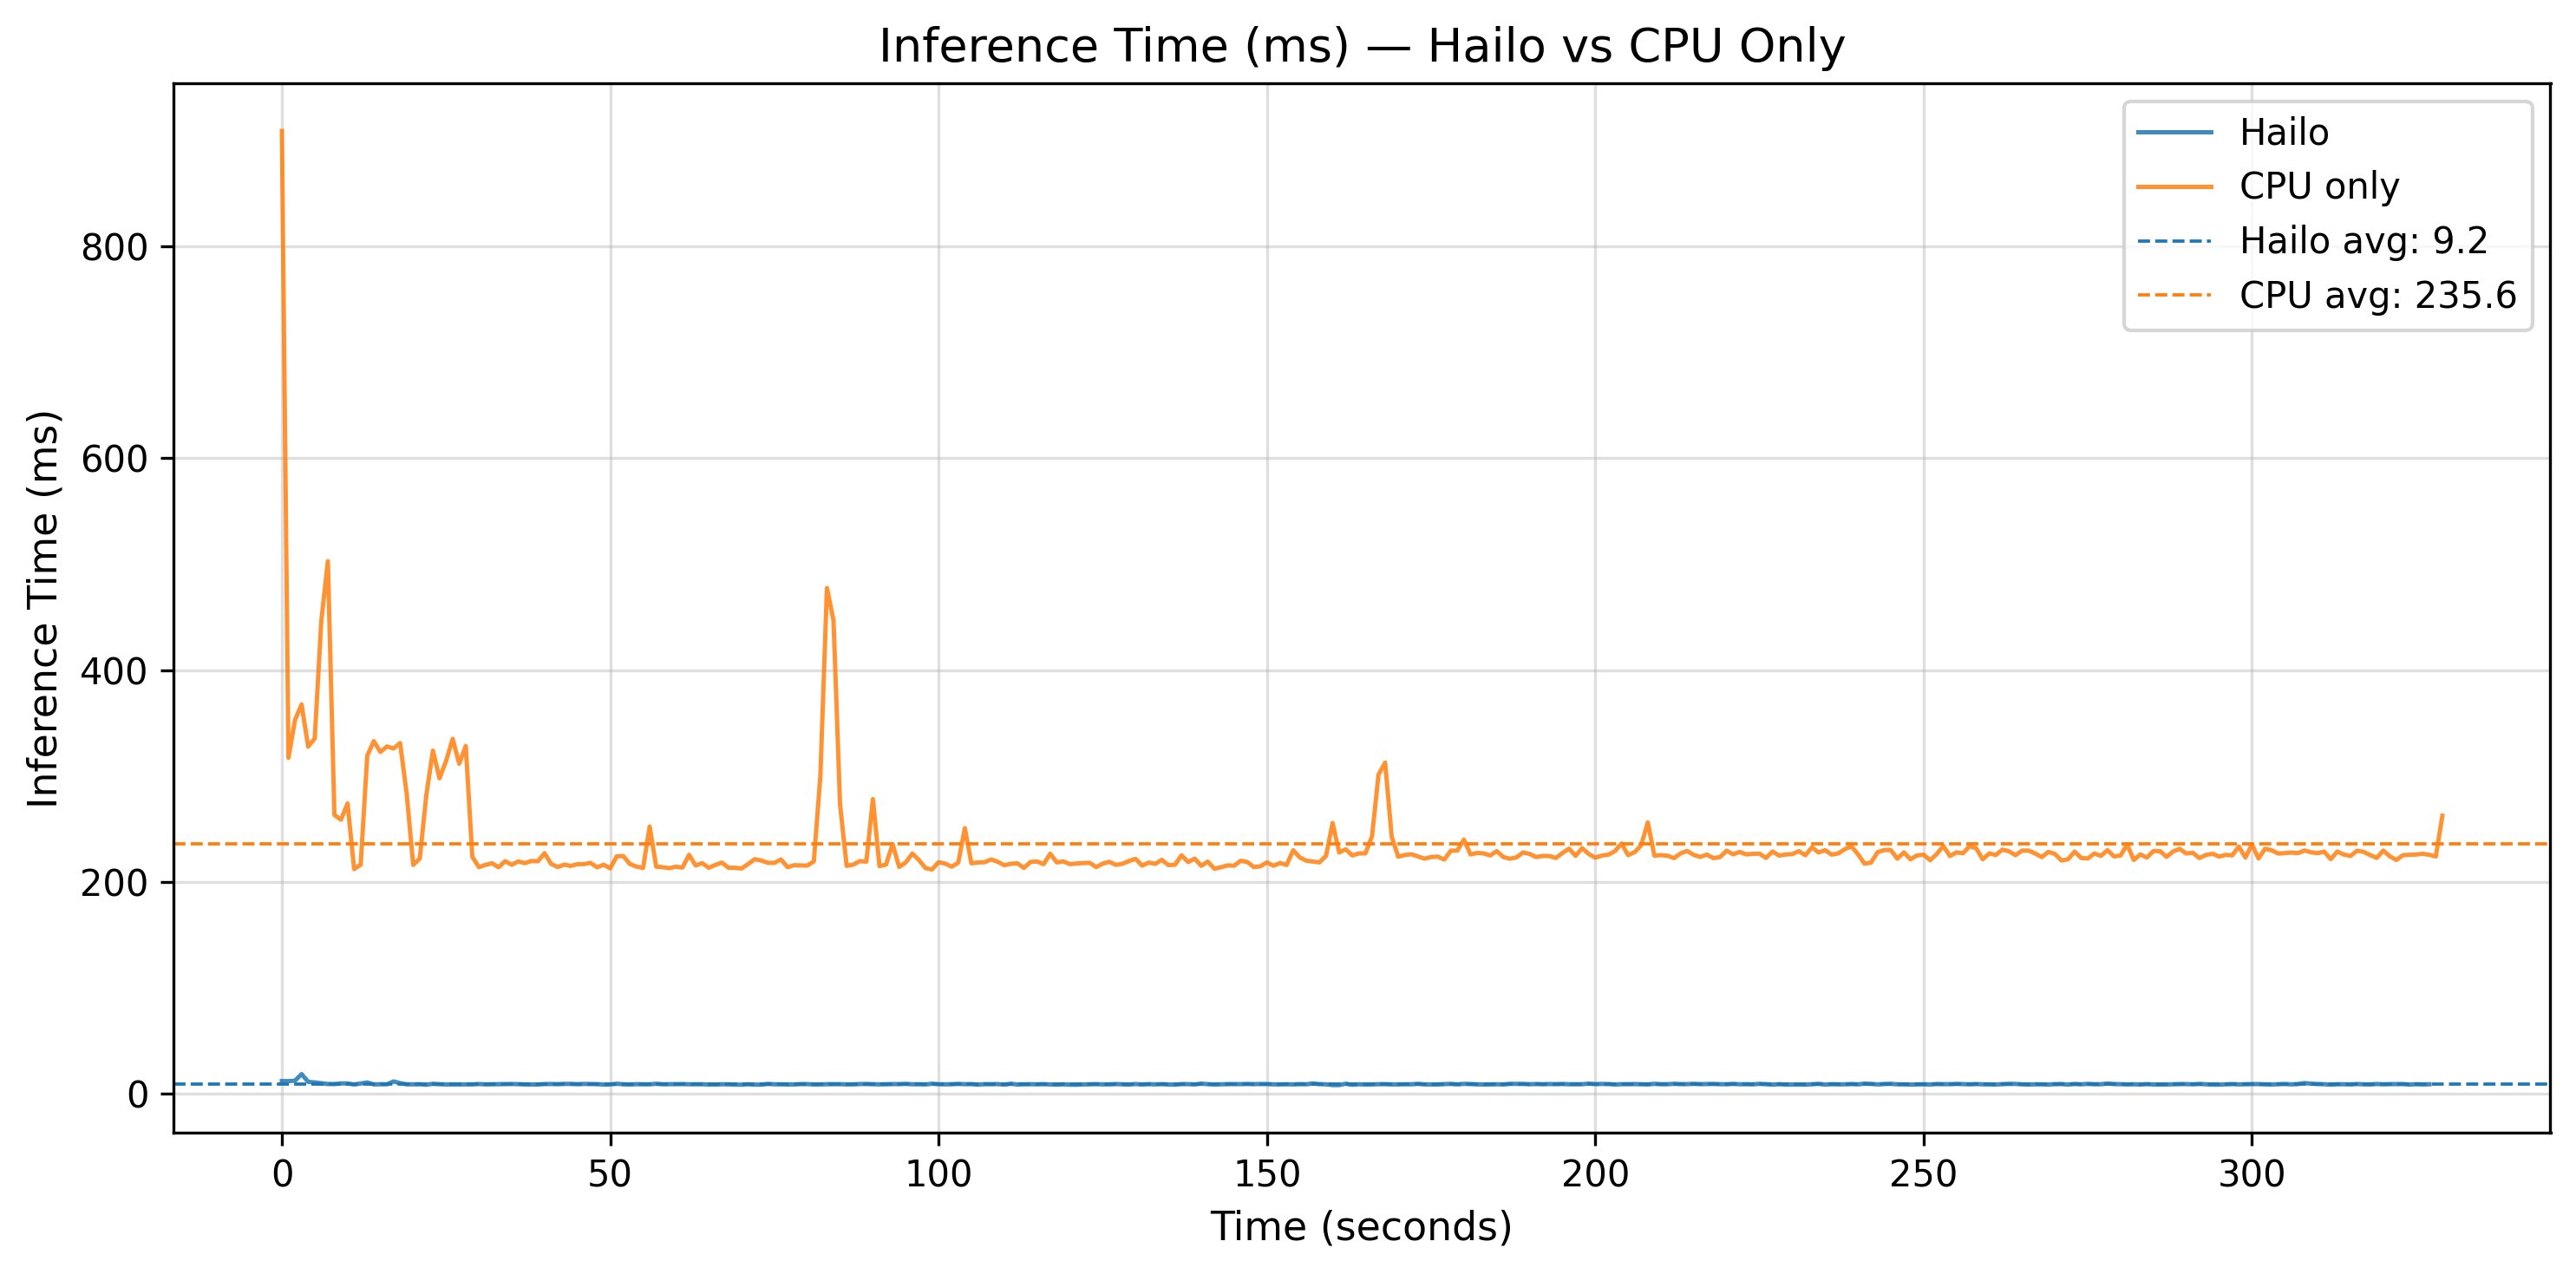
\includegraphics[width=0.95\linewidth]{Figures/Andreas/Hardware/avg_inference_ms_comparison.png}
    \caption[Interference Comparison]{Interference comparison between using the HAILO chip and CPU only, with the HAILO average interefence time being 9.2ms and with CPU only being 235.6ms.}
    \label{fig:Interference_comp}
\end{figure}

It was found that the CPU usage with the HAILO chip was at 29.7\% on average, where as without the CPU usage was found to be 92.5\% on average.(\ref{fig:cpu_usage_comparison}) Similarily the average CPU temperature with the HAILO chip was found to be 54.1 $C\degree$ where as with CPU only the average temperature rose to an average of 71 $C\degree$ (\ref{fig:cpu_temp_comparison})

\begin{figure}[H]
    \centering
    \begin{subfigure}[b]{0.48\textwidth}
        \centering
        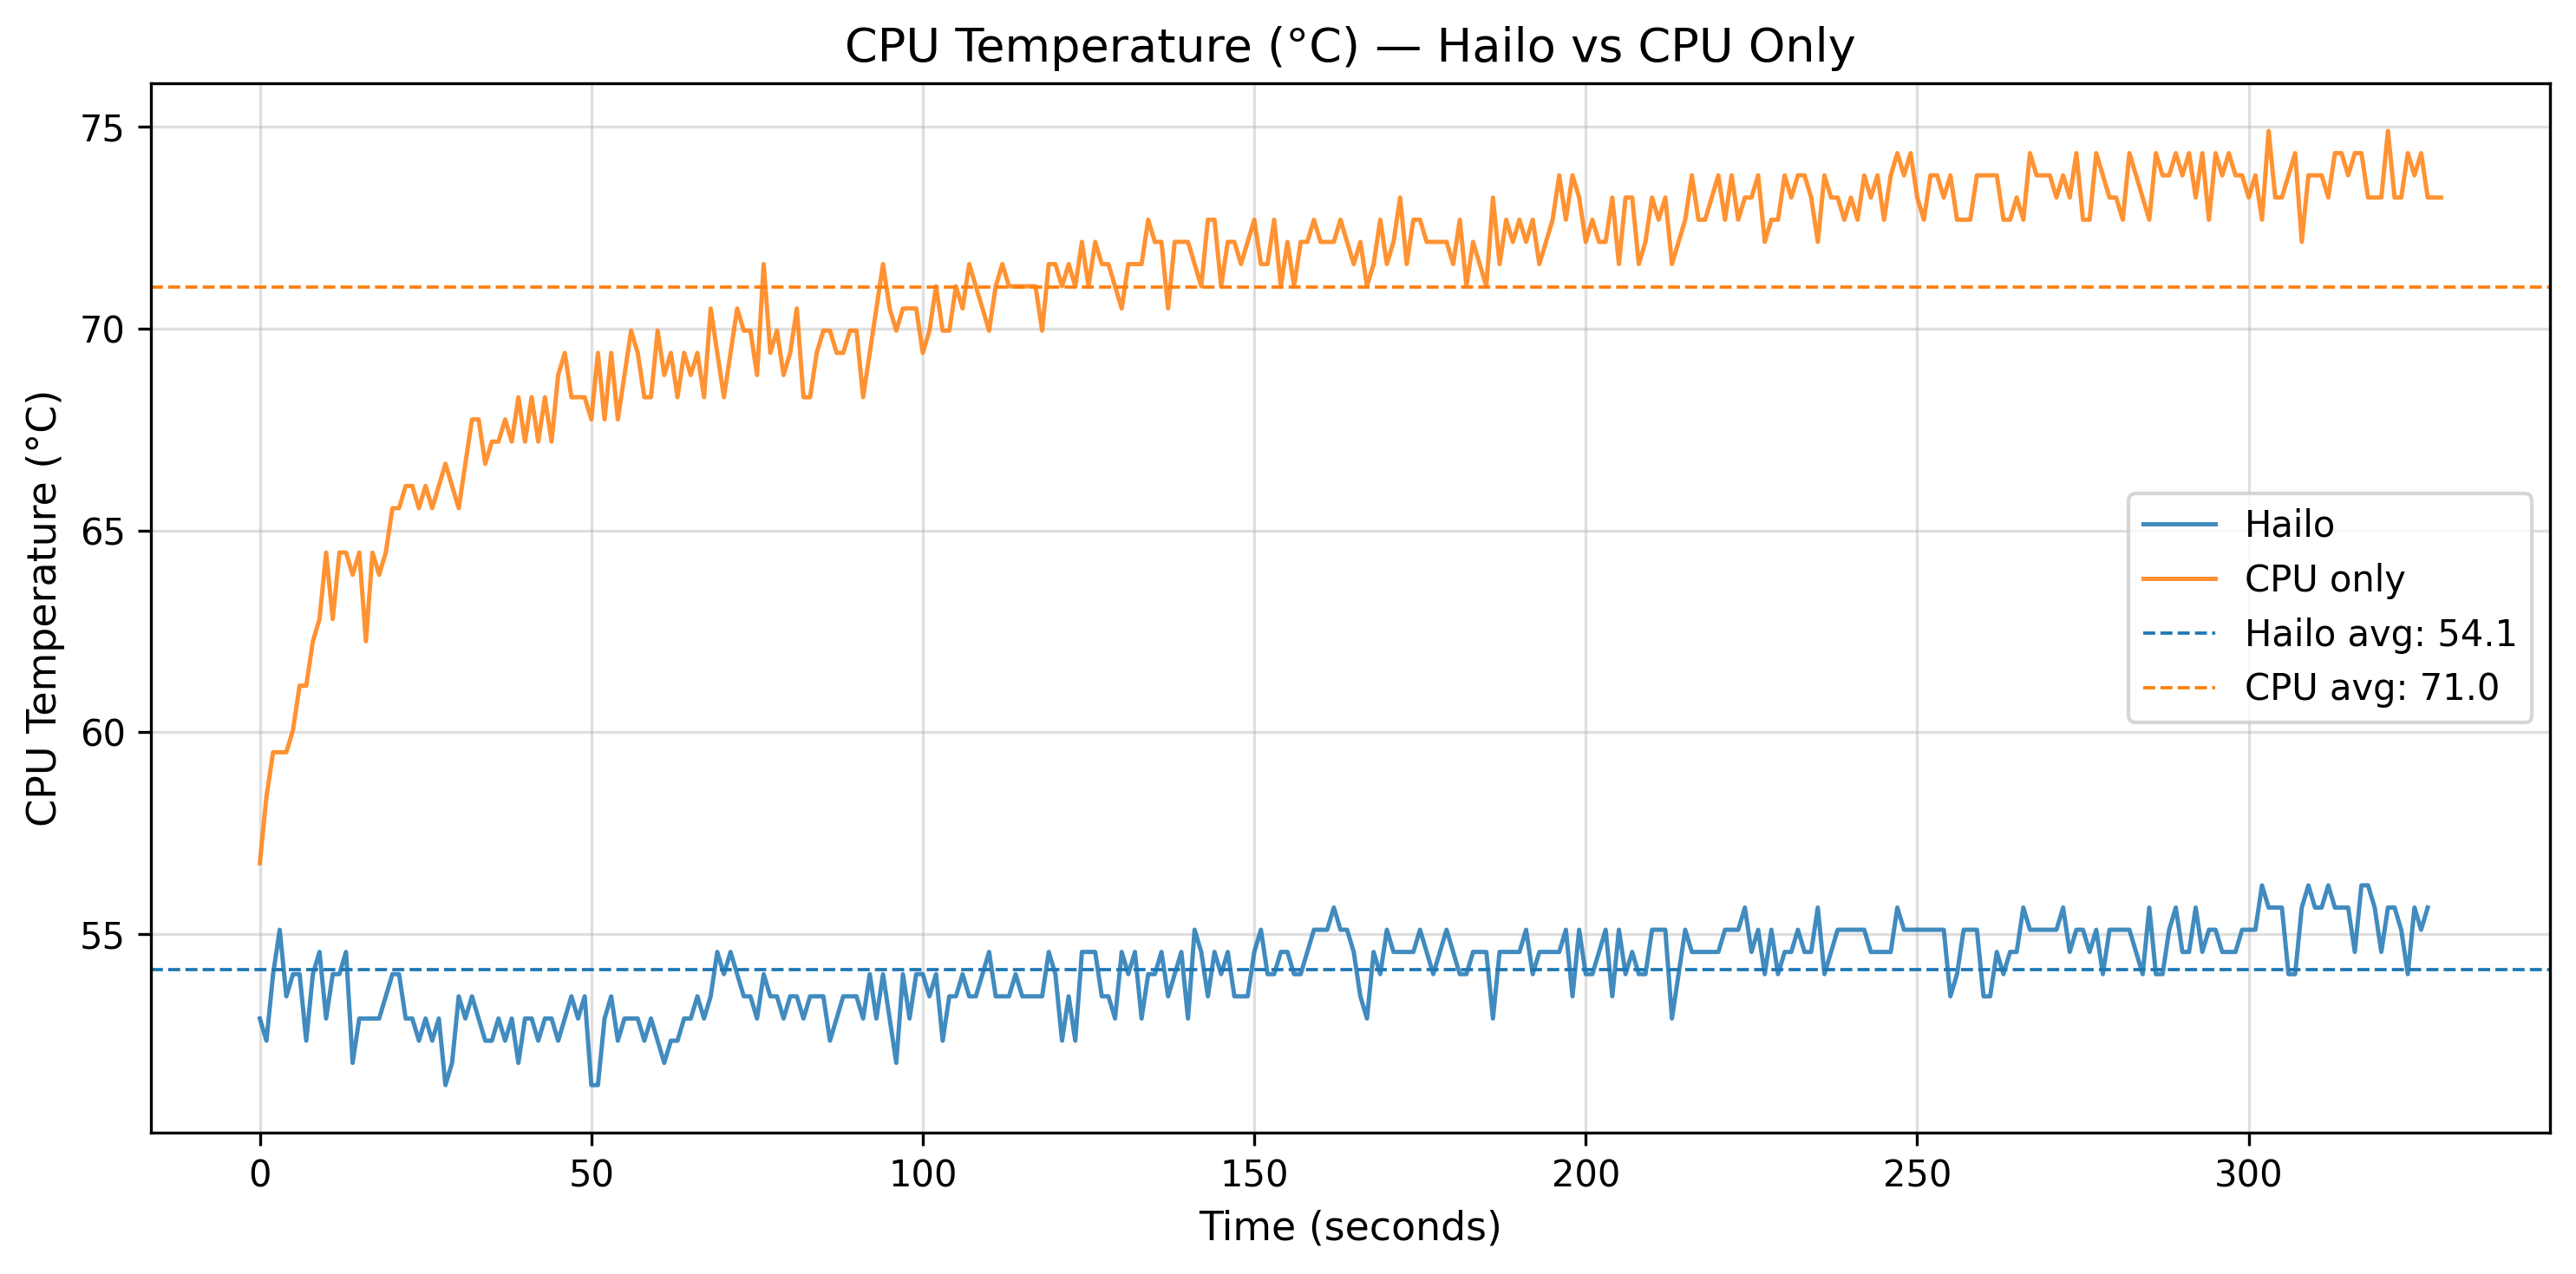
\includegraphics[width=\textwidth]{Figures/Andreas/Hardware/cpu_temp_c_comparison.png}
        \caption{CPU temperature comparison}
        \label{fig:cpu_temp_comparison}
    \end{subfigure}
    \hfill
    \begin{subfigure}[b]{0.48\textwidth}
        \centering
        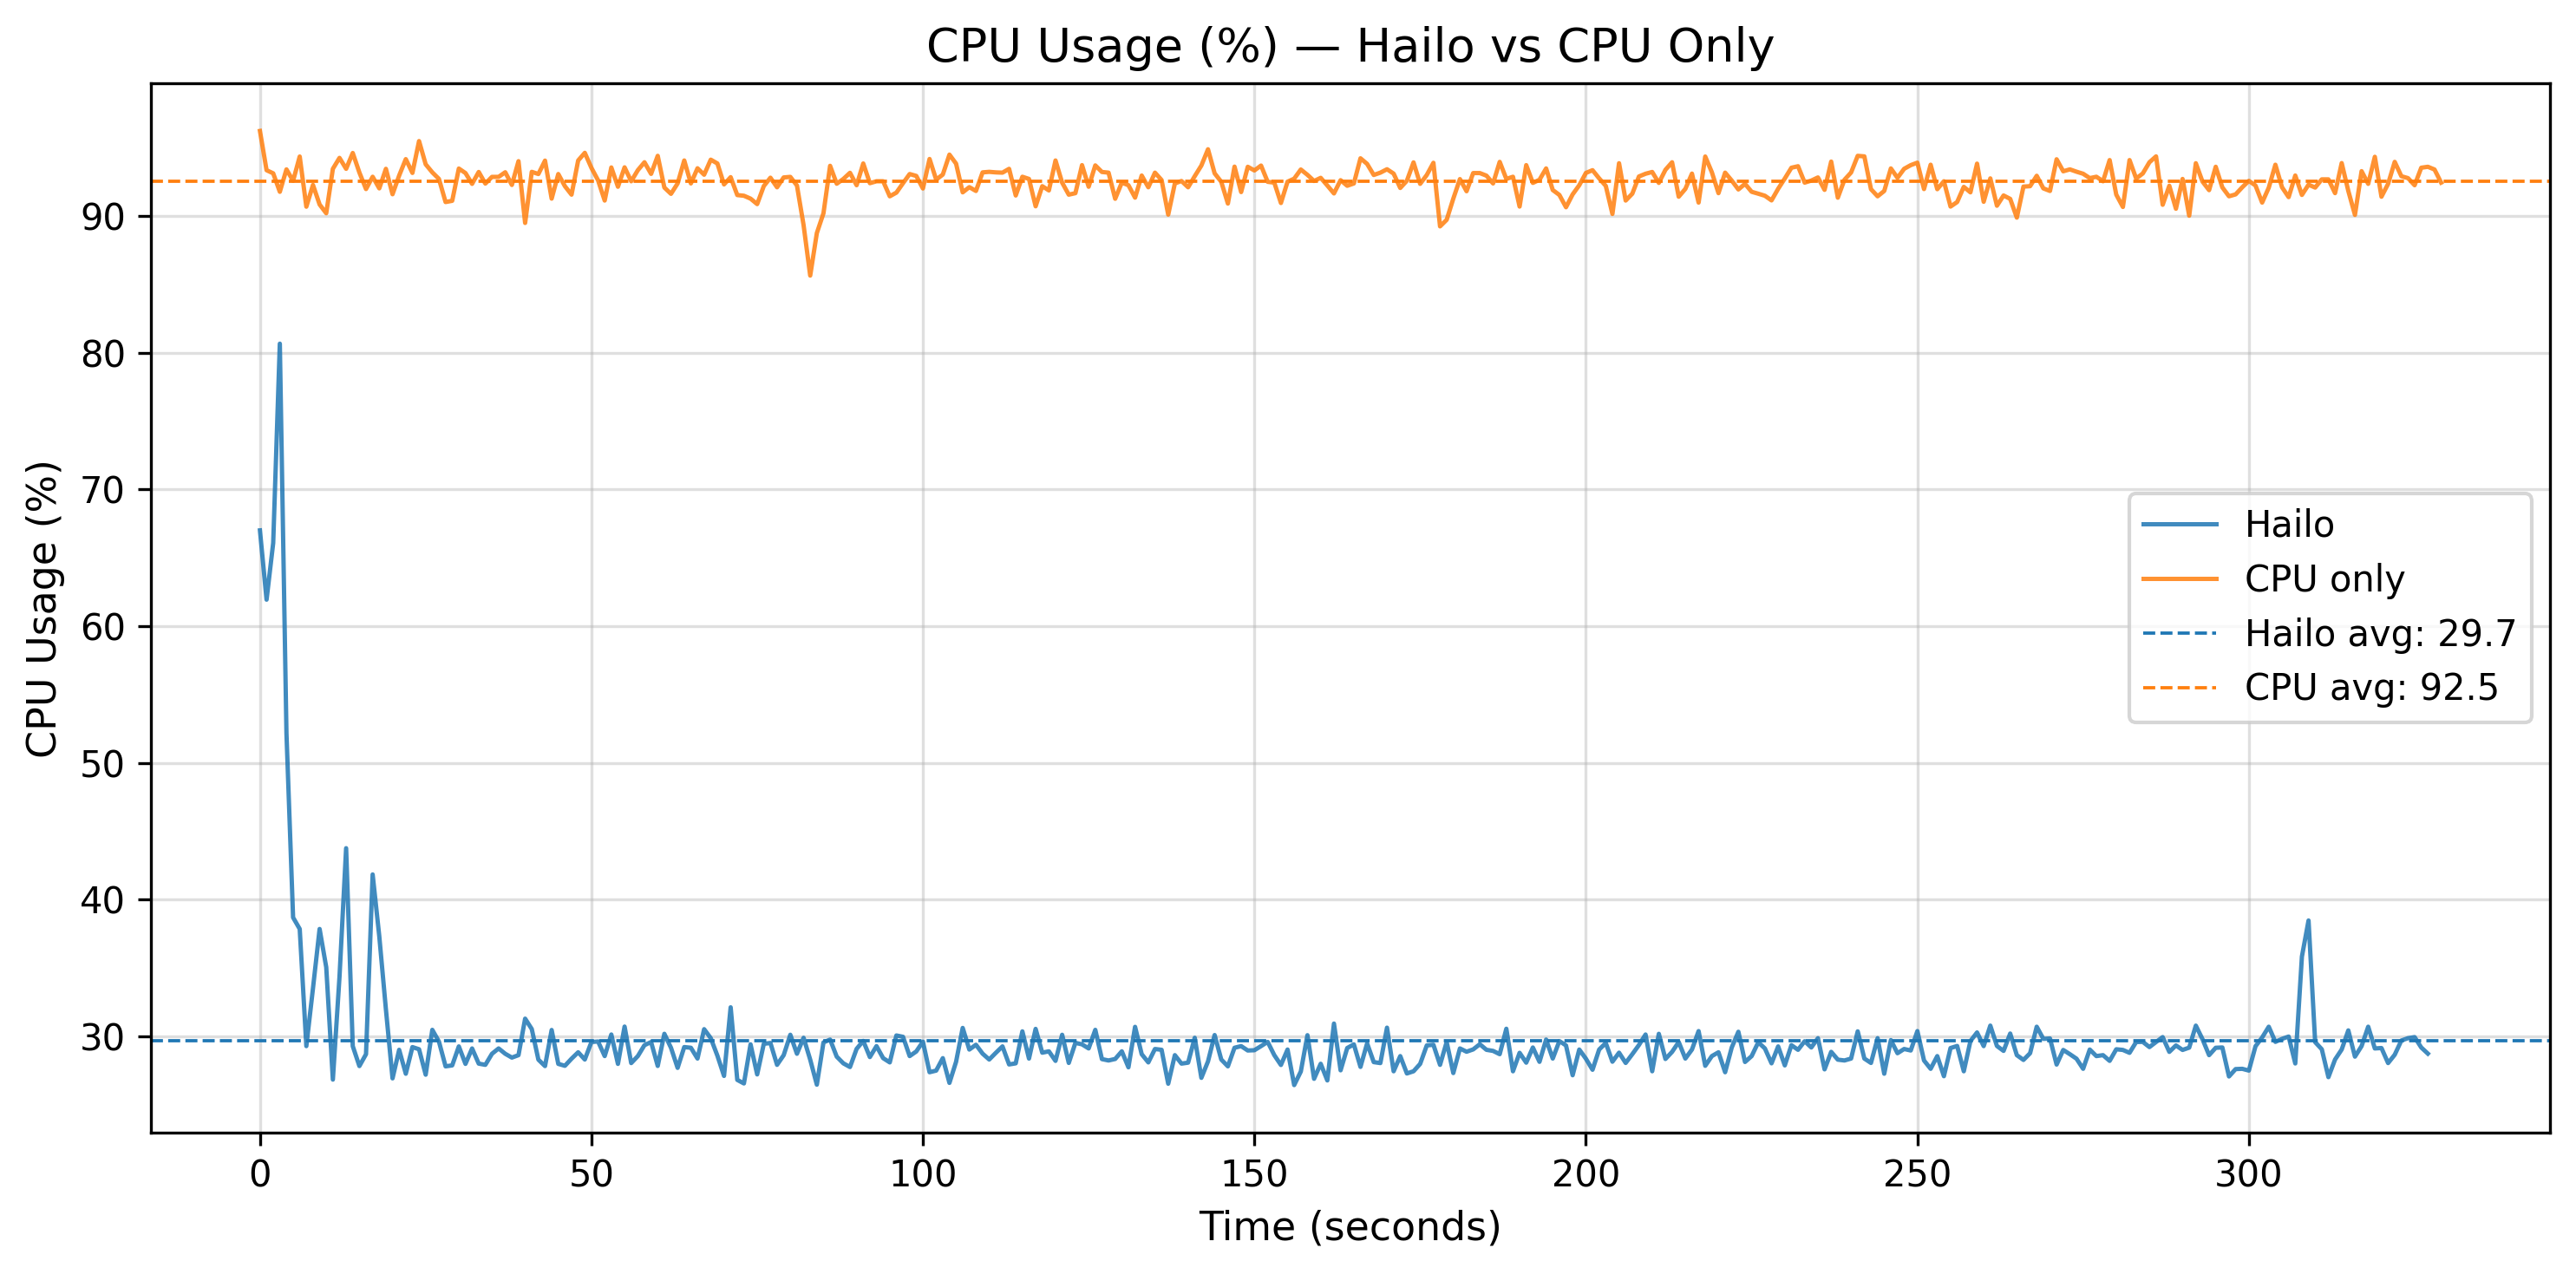
\includegraphics[width=\textwidth]{Figures/Andreas/Hardware/cpu_usage_pct_comparison.png}
        \caption{CPU usage comparison}
        \label{fig:cpu_usage_comparison}
    \end{subfigure}
    \caption{CPU temperature and usage during Hailo and CPU-only inference pipelines. The average CPU temperature and usage with the HAILO chip were 54.1 C$\degree$   and 29.7 \% respectively}
    \label{fig:cpu_comparison}
\end{figure}

The RAM usage was found to be similar both with and without the HAILO chip (\ref{fig:RAM Usage})

\begin{figure}[H]
    \centering
    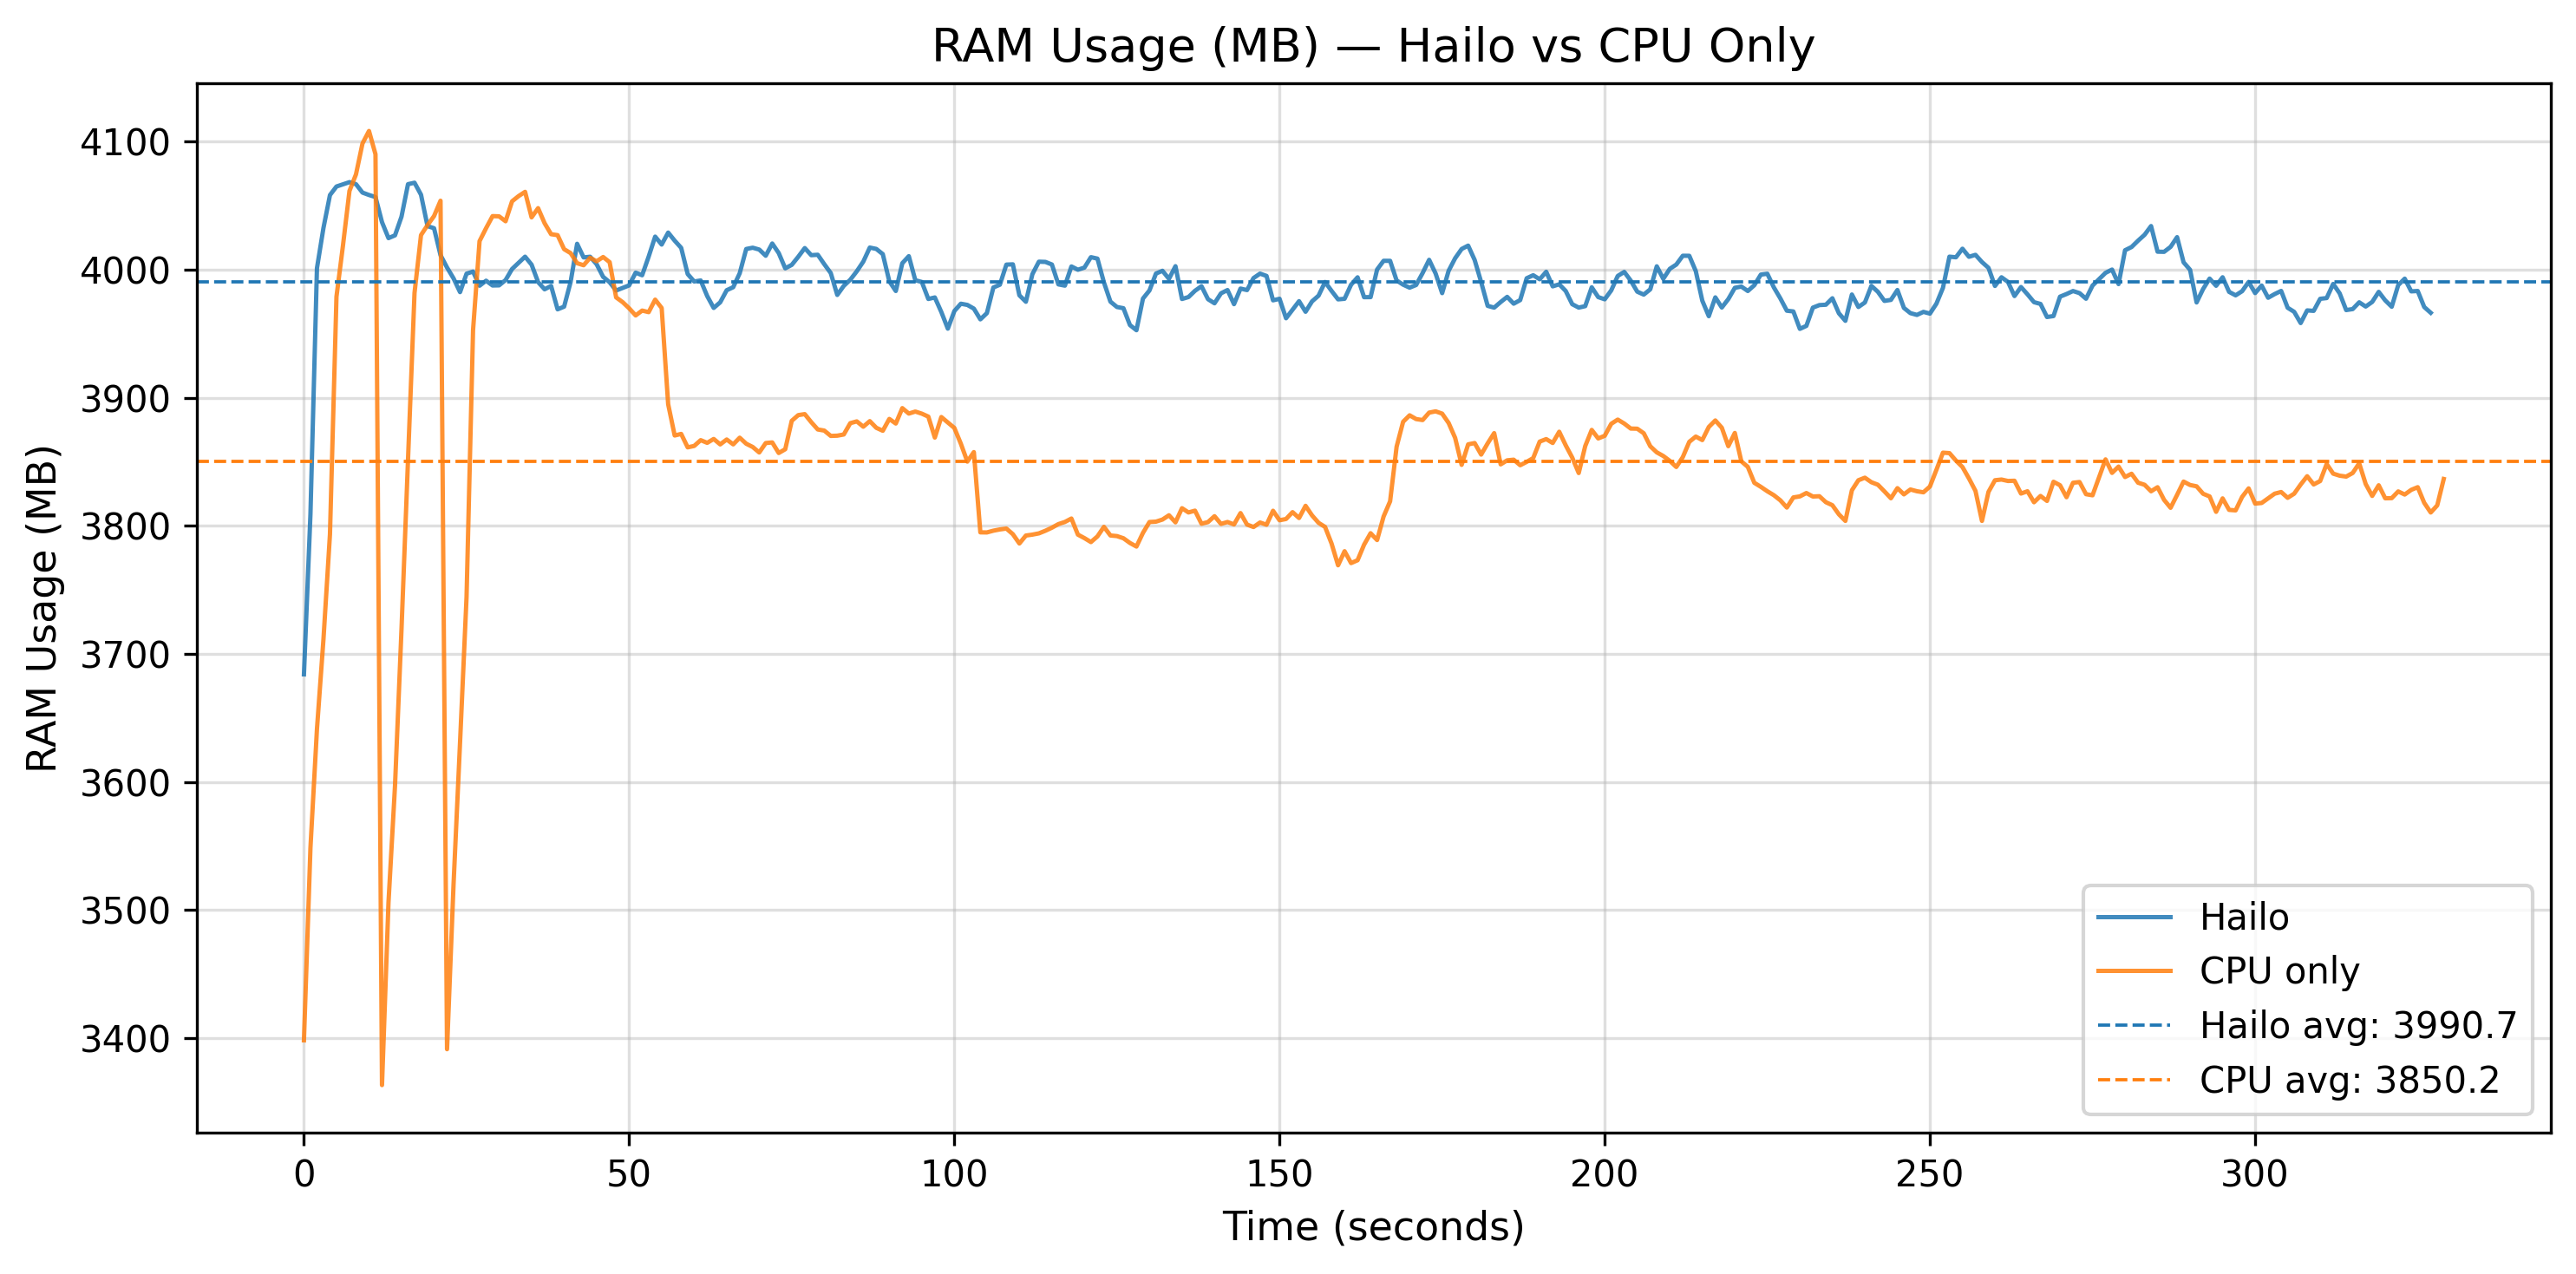
\includegraphics[width=0.95\linewidth]{Figures/Andreas/Hardware/ram_used_mb_comparison.png}
    \caption[RAM usage]{RAM usage on the RPI with and without the HAILO AI chip. }
    \label{fig:RAM Usage}
\end{figure}



\section{YOLO results}
\subsection{Training results}
The training on the final YOLO model lasted for about 11.5 hours with the model converging on 43 epochs with each epoch taking around 16 minutes to complete. The three main training losses, box, classification and DFL declined consistently throughout the training (fig: \ref{fig:pYolo_results}). The val box loss has a slight increase after epoct 25 (0.02), indicating some overfitting on the bounding box regression (fig: \ref{fig:pYolo_results}). The val classification loss has a high scale compared to the training classification loss (fig: \ref{fig:pYolo_results}).

\begin{figure}[H]
    \centering
    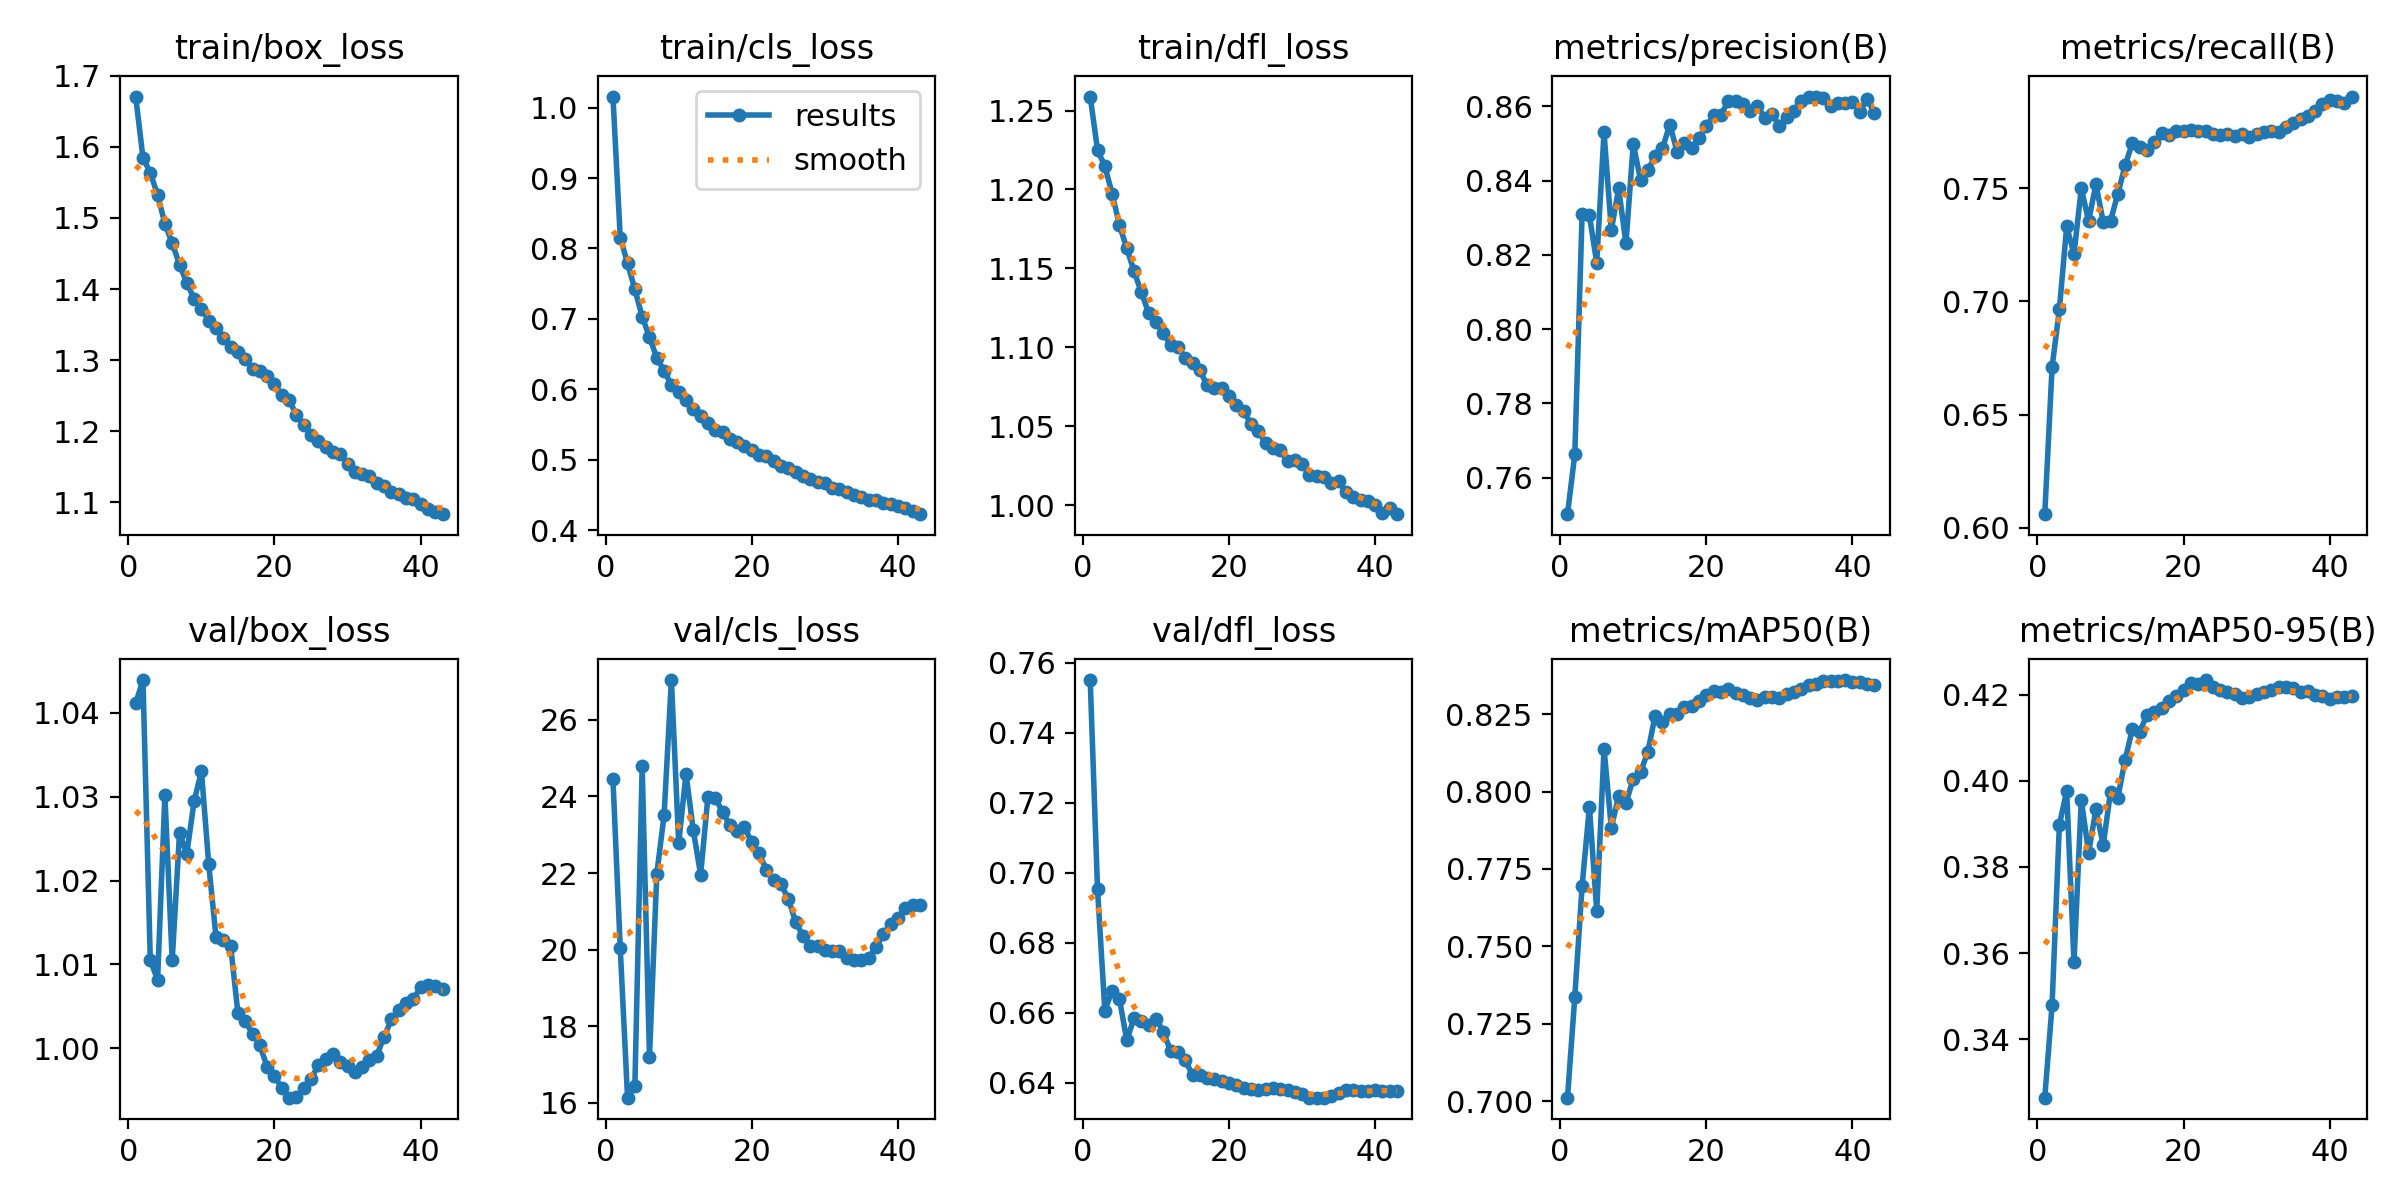
\includegraphics[width=0.95\linewidth]{Figures/Andreas/YOLO/results.png}
    \caption[YOLO results]{YOLOv8n training and validation loss curves over 43 epochs. The box, classification, and distribution focal loss (DFL) all decline consistently during training. A slight increase in validation box loss after epoch 25 indicates marginal overfitting on bounding box regression. The validation classification loss operates at a higher scale than the training classification loss, attributable to the 2,750 background-only images in the validation set actively penalising false detections. The best mAP@0.50 and mAP@0.50:0.95 scores were 0.835 and 0.420 respectively.}
    \label{fig:pYolo_results}
\end{figure}

The best $mAP_{50}$ score was at 0.835 and the $mAP_{50:95}$ was at 0.420 (fig: \ref{tab:yolo_detection_performance}). 

\begin{table}[H]
    \centering
    \caption{YOLOv8N detection performance on the DroneDetectionDataset validation set.}
    \label{tab:yolo_detection_performance}
    \begin{tabular}{lc}
        \toprule
        \textbf{Metric} & \textbf{Value} \\
        \midrule
        Precision           & 0.862 \\
        Recall              & 0.790 \\
        F1 Score            & 0.810 \\
        mAP@0.50            & 0.835 \\
        mAP@0.50:0.95       & 0.420 \\
        Optimal confidence threshold & 0.571 \\
        \bottomrule
    \end{tabular}
\end{table}

The confusion matrix shows a true positive rate of $88\%$ (fig: \ref{fig:Yolo_confusion_matrix}).

\begin{figure}[H]
    \centering
    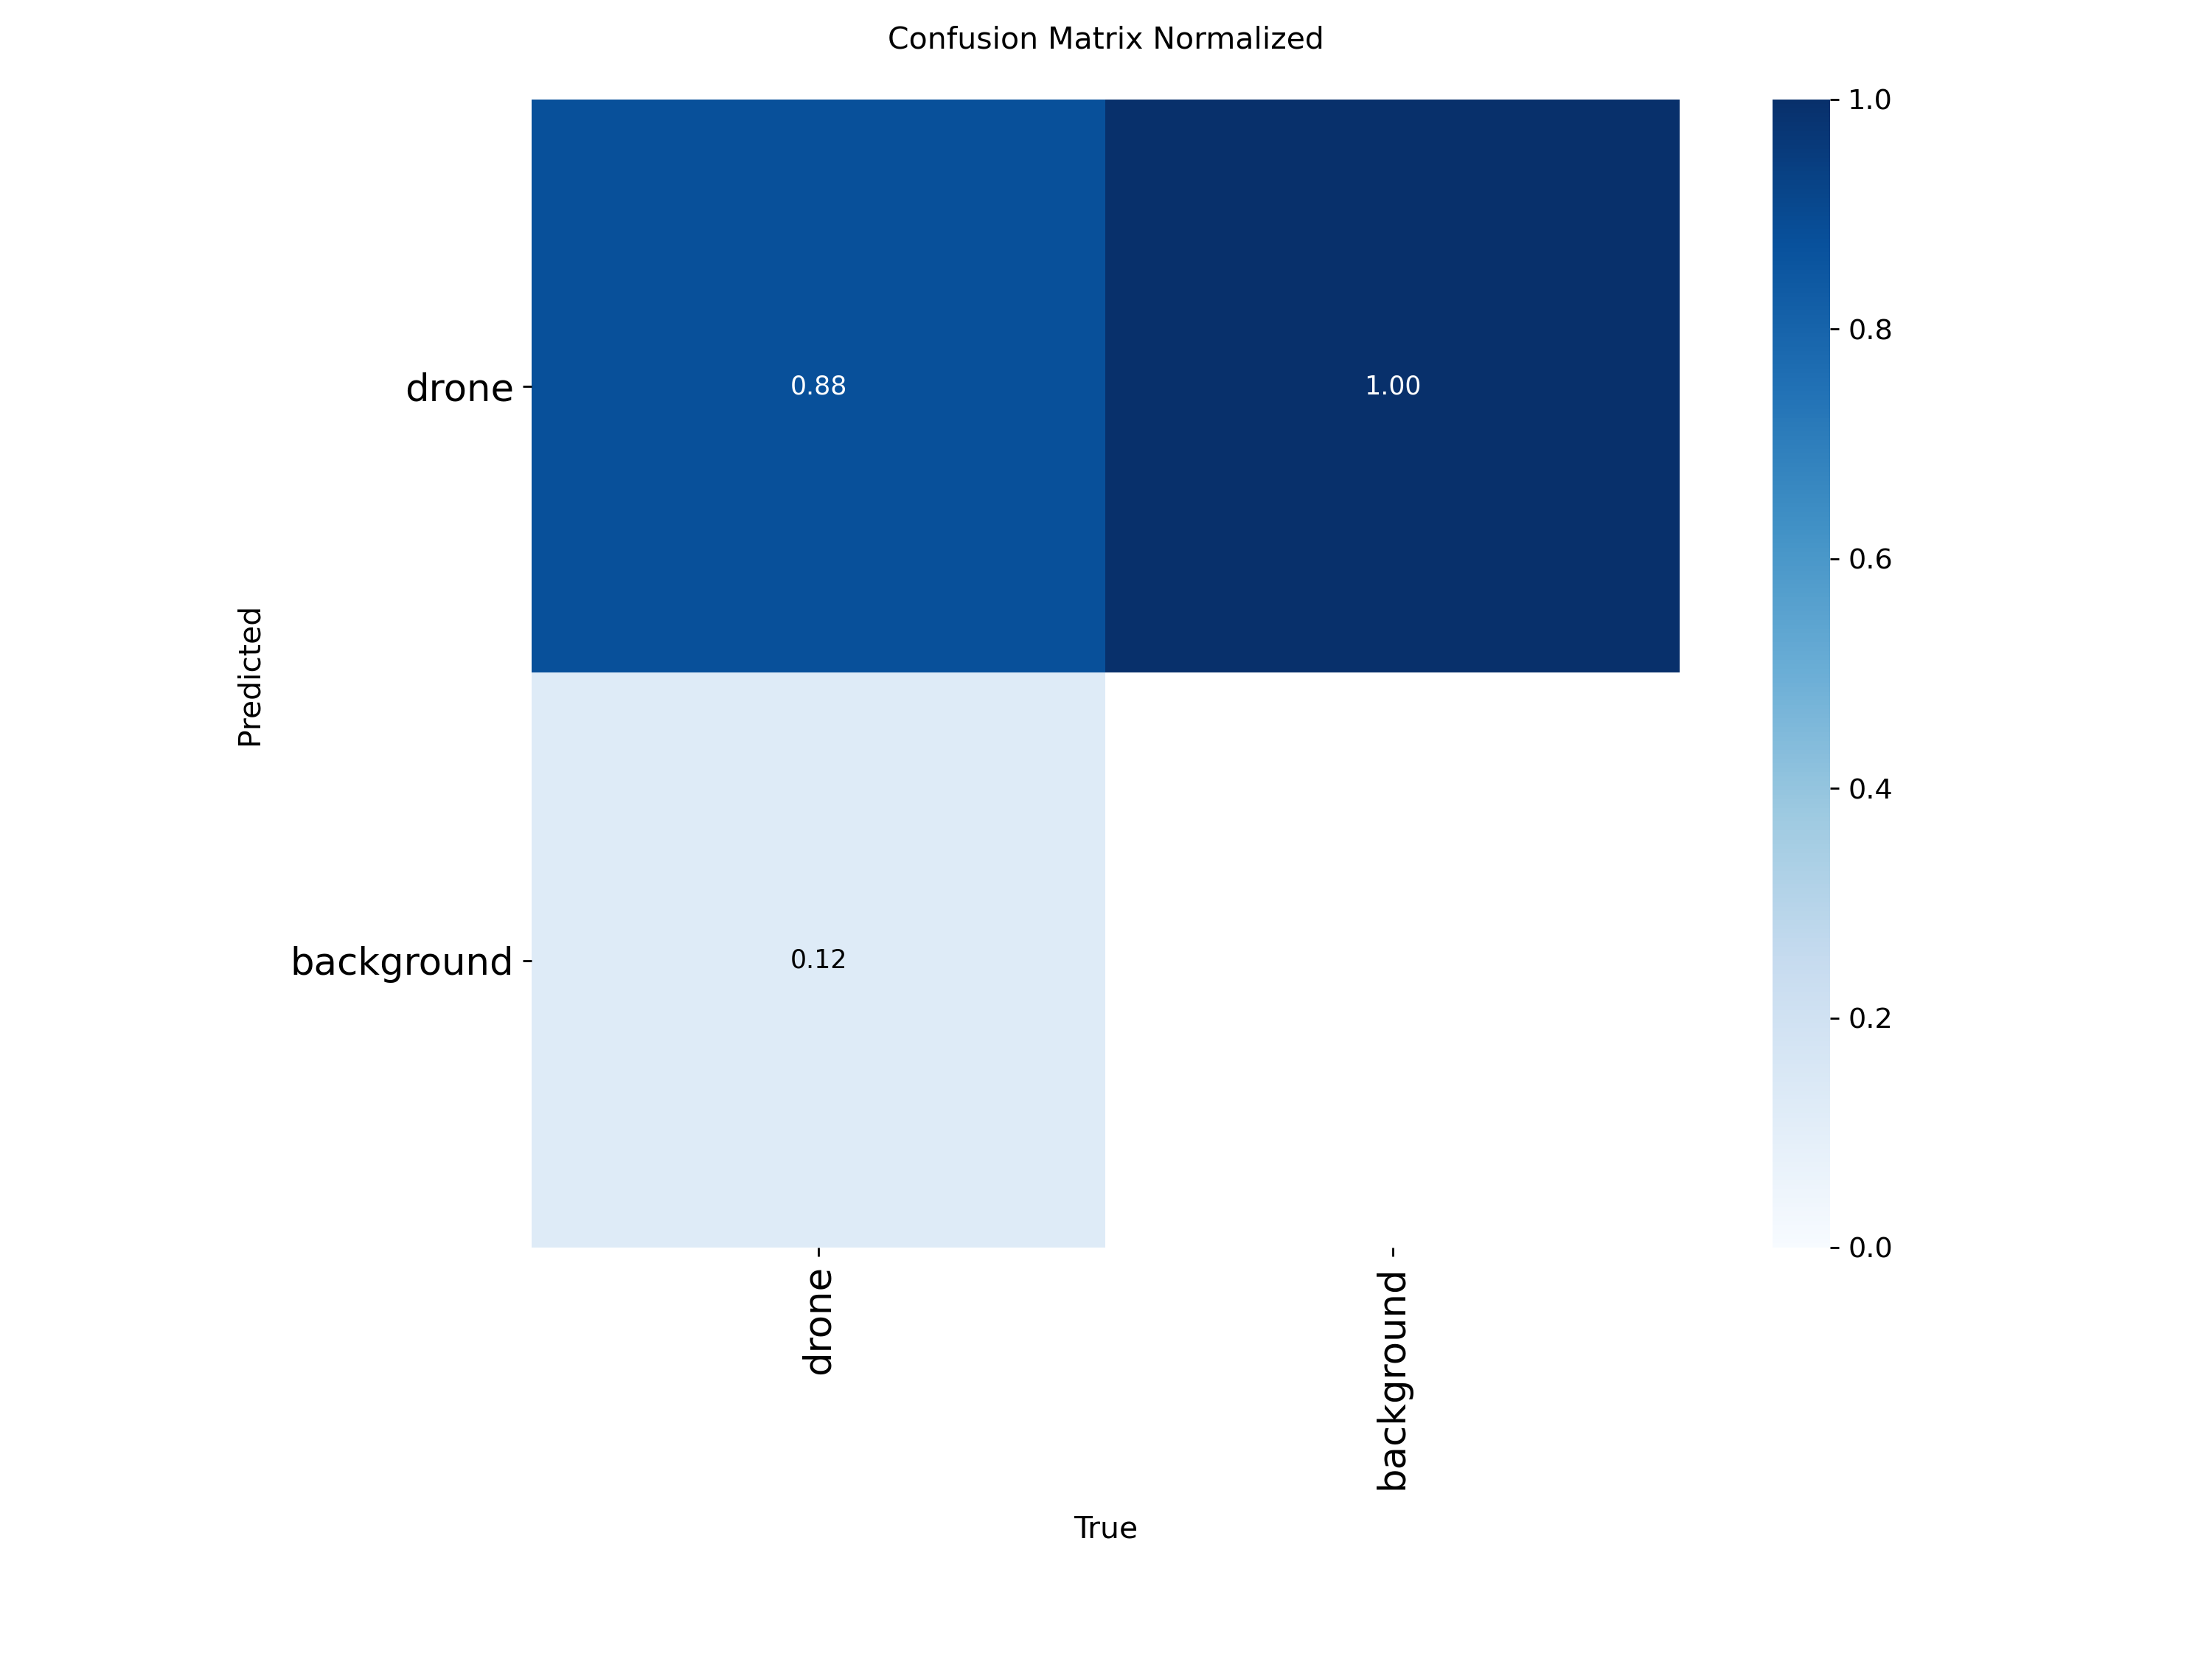
\includegraphics[width=0.95\linewidth]{Figures/Andreas/YOLO/confusion_matrix_normalized.png}
    \caption[YOLO confusion matrix normalized]{Normalised confusion matrix for the YOLOv8n model evaluated on the DroneDetectionDataset validation set. The model achieves a true positive rate of 88\%, with the remaining 12\% of drone instances going undetected. All background instances received a non-zero detection at some confidence level, indicating some false positives, though these are well-controlled at the recommended operating threshold of 0.571}
    \label{fig:Yolo_confusion_matrix}
\end{figure}

The PR curve shows an mAP@0.5 of 0.832. The curve maintains near-perfect precision (>0.95) up to a recall of approximately 0.65, after which precision drops steeply. This indicates the model is highly reliable at moderate recall thresholds but begins trading precision for recall aggressively beyond 0.75 recall. The area under the curve (0.832) confirms strong overall detection performance on a challenging real-world benchmark.(fig: \ref{fig:f1_curve})

The F1 curve peaks at 0.81 at a confidence threshold of 0.571. This is the recommended operating threshold for deployment — detections below this confidence should be discarded. The curve is broad and relatively flat between confidence values of 0.35 and 0.70, meaning the model is robust to moderate threshold adjustments without significant performance loss. Beyond 0.75 confidence the F1 score drops sharply as the model becomes too conservative and misses genuine drones. (fig: \ref{fig:pr_curve}).


\begin{figure}[H]
    \centering
    \begin{subfigure}[b]{0.48\textwidth}
        \centering
        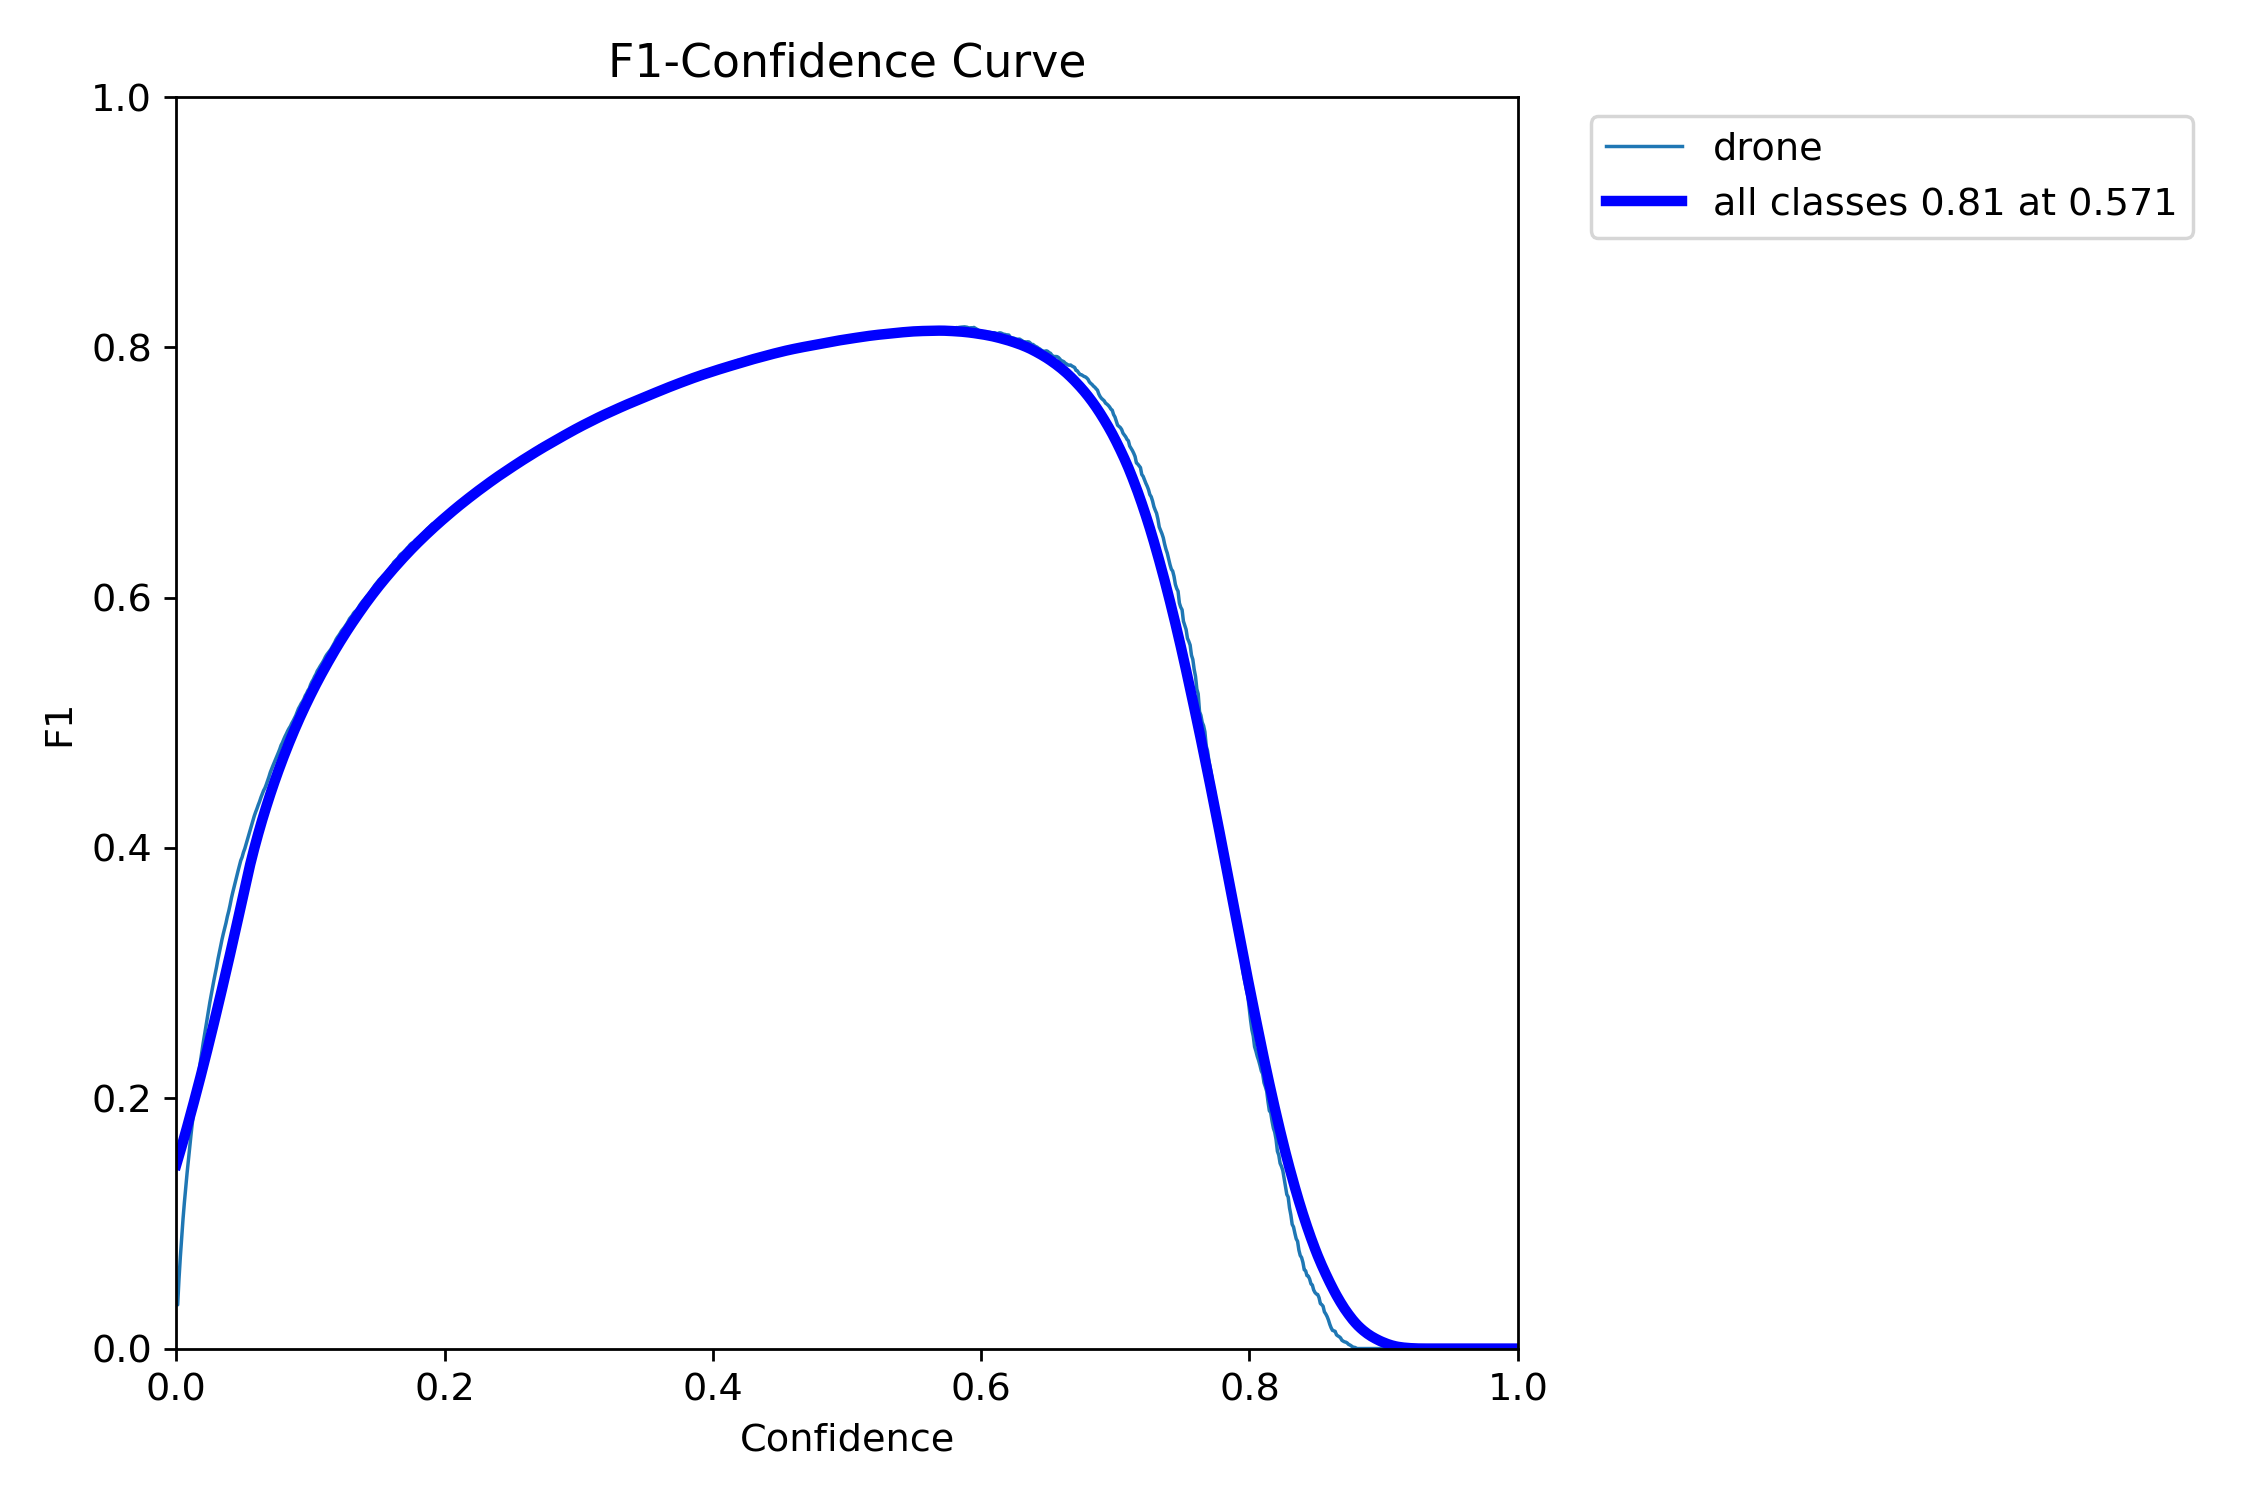
\includegraphics[width=\textwidth]{Figures/Andreas/YOLO/BoxF1_curve.png}
        \caption{F1 score curve}
        \label{fig:f1_curve}
    \end{subfigure}
    \hfill
    \begin{subfigure}[b]{0.48\textwidth}
        \centering
        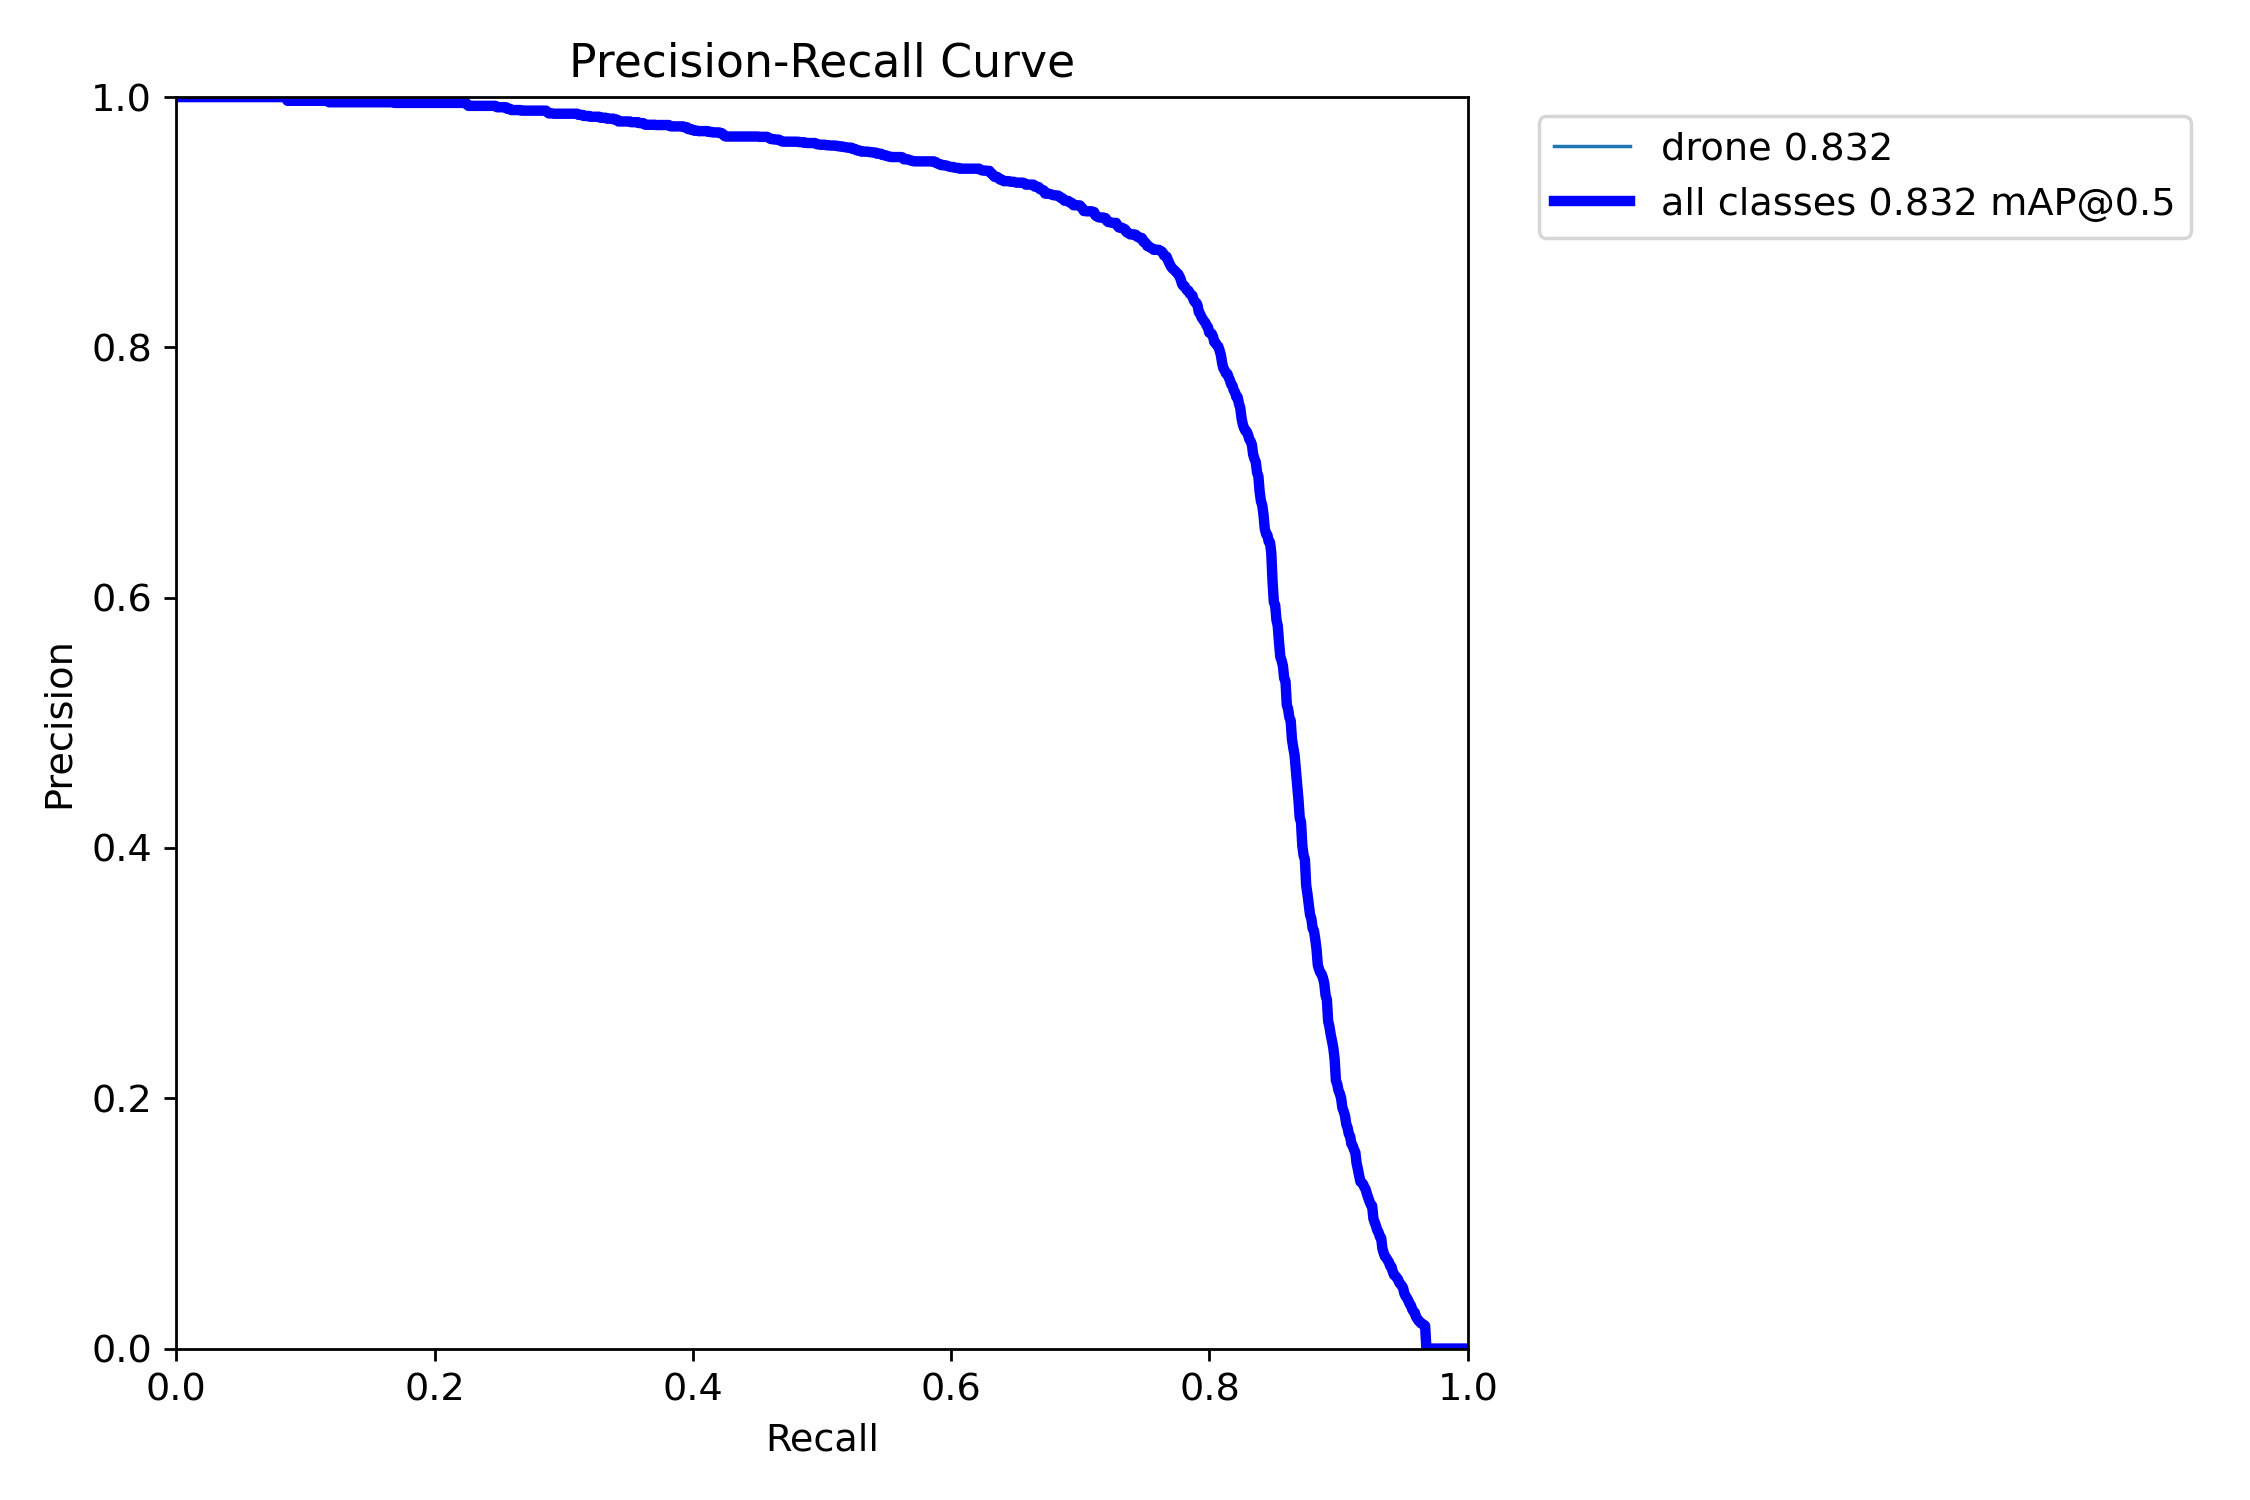
\includegraphics[width=\textwidth]{Figures/Andreas/YOLO/BoxPR_curve.png}
        \caption{Precision-recall curve}
        \label{fig:pr_curve}
    \end{subfigure}
    \caption[F1 and PR curves]{ Precision-recall curve for the YOLOv8n drone detector, showing an mAP@0.50 of 0.832. The model maintains near-perfect precision above 0.95 up to a recall of approximately 0.65, after which precision degrades sharply as the model trades specificity for coverage. (b) F1-confidence curve peaking at 0.81 at a confidence threshold of 0.571, which is used as the recommended deployment threshold. The curve remains broad and relatively flat between confidence values of 0.35 and 0.70, indicating robustness to moderate threshold adjustments.}
    \label{fig:f1_pr_curves}
\end{figure}

\subsection{Video drone detection results}

From the tested videos it was found that overall the YOLO model sucessfully detected the drones in a variety of backgrounds and distances without too many false positives. However in the floureon FPV video (\cite{floureon2017}), it was observed that the model consistently failed to detect the drone when the background was occupied by dark leaved trees (\ref{fig:video_comparison}). 

\begin{figure}[H]
    \centering
    \begin{subfigure}[b]{0.48\textwidth}
        \centering
        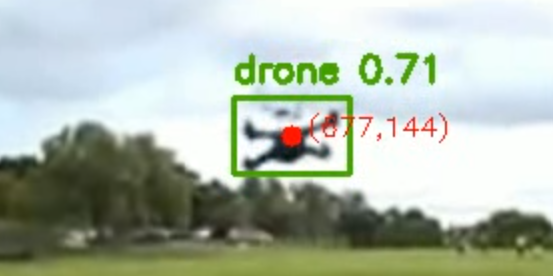
\includegraphics[width=\textwidth]{Figures/Andreas/YOLO/Video_NO_trees.png}
        \caption{Detection without trees}
        \label{fig:video_no_trees}
    \end{subfigure}
    \hfill
    \begin{subfigure}[b]{0.48\textwidth}
        \centering
        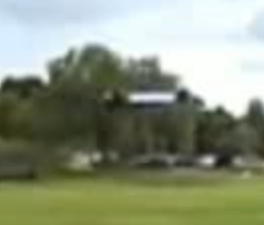
\includegraphics[width=\textwidth]{Figures/Andreas/YOLO/Video_with_trees.png}
        \caption{Detection with trees}
        \label{fig:video_with_trees}
    \end{subfigure}
    \caption[Video detection comparison]{Screenshots taken from one of the videos showcasing the YOLO model.}
    \label{fig:video_comparison}
\end{figure}

The video with the most false positives was found to be the TED talk bideo by Rafaello D'Andrea (\cite{dandrea2016}). In the video there are multiple instances of the YOLO model mistaking a person, as well as a TV (\ref{fig:ted_detections}).

\begin{figure}[H]
    \centering
    \begin{subfigure}[b]{0.48\textwidth}
        \centering
        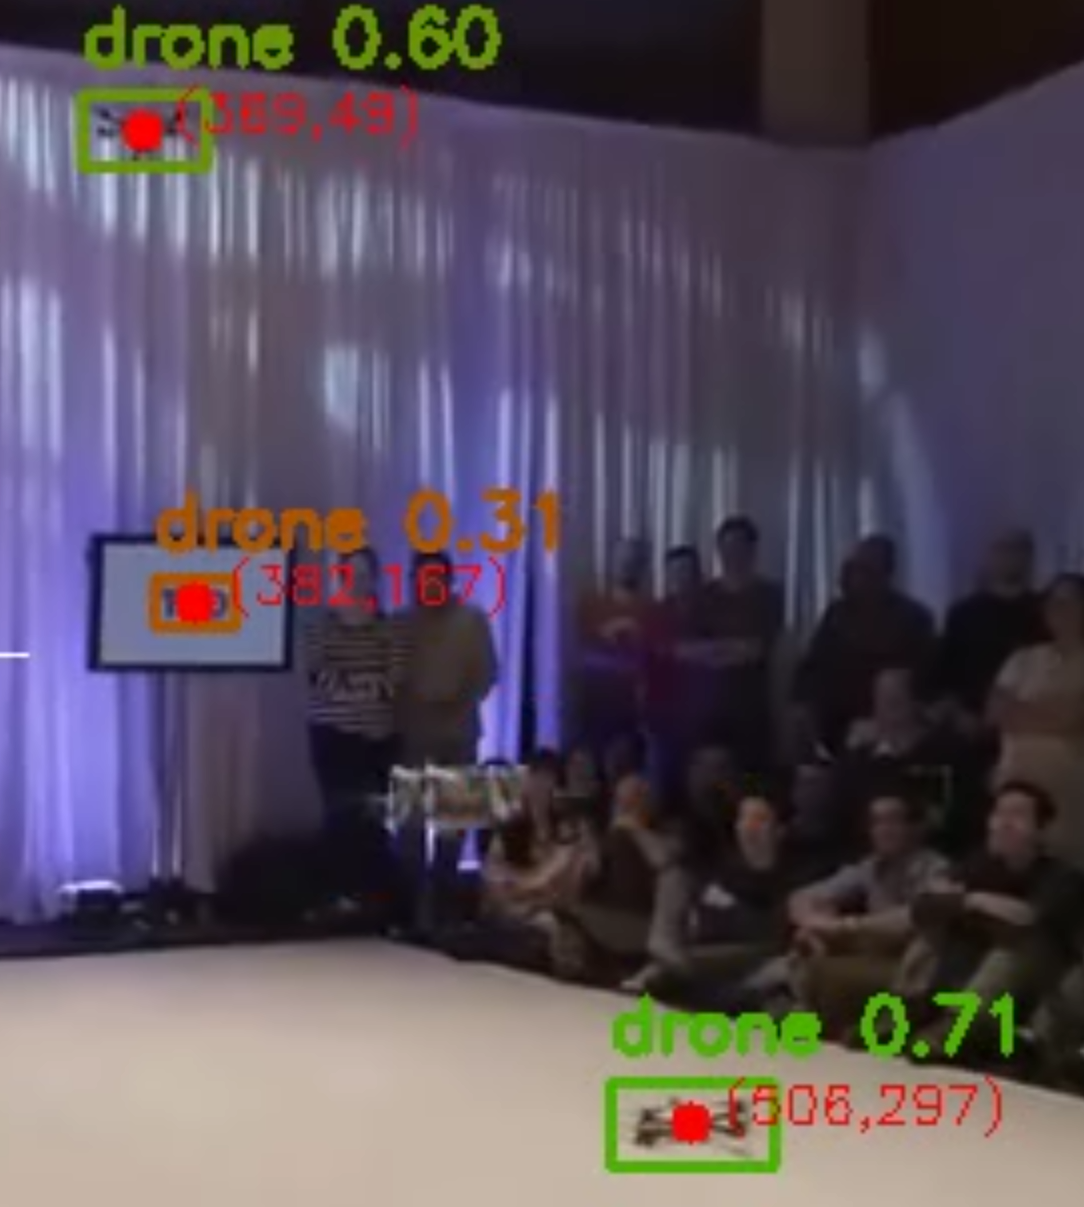
\includegraphics[width=\textwidth]{Figures/Andreas/YOLO/TED_TPandFP.png}
        \caption{True positive and false positive, and a drone thats not detected at all}
        \label{fig:ted_tp_fp}
    \end{subfigure}
    \hfill
    \begin{subfigure}[b]{0.48\textwidth}
        \centering
        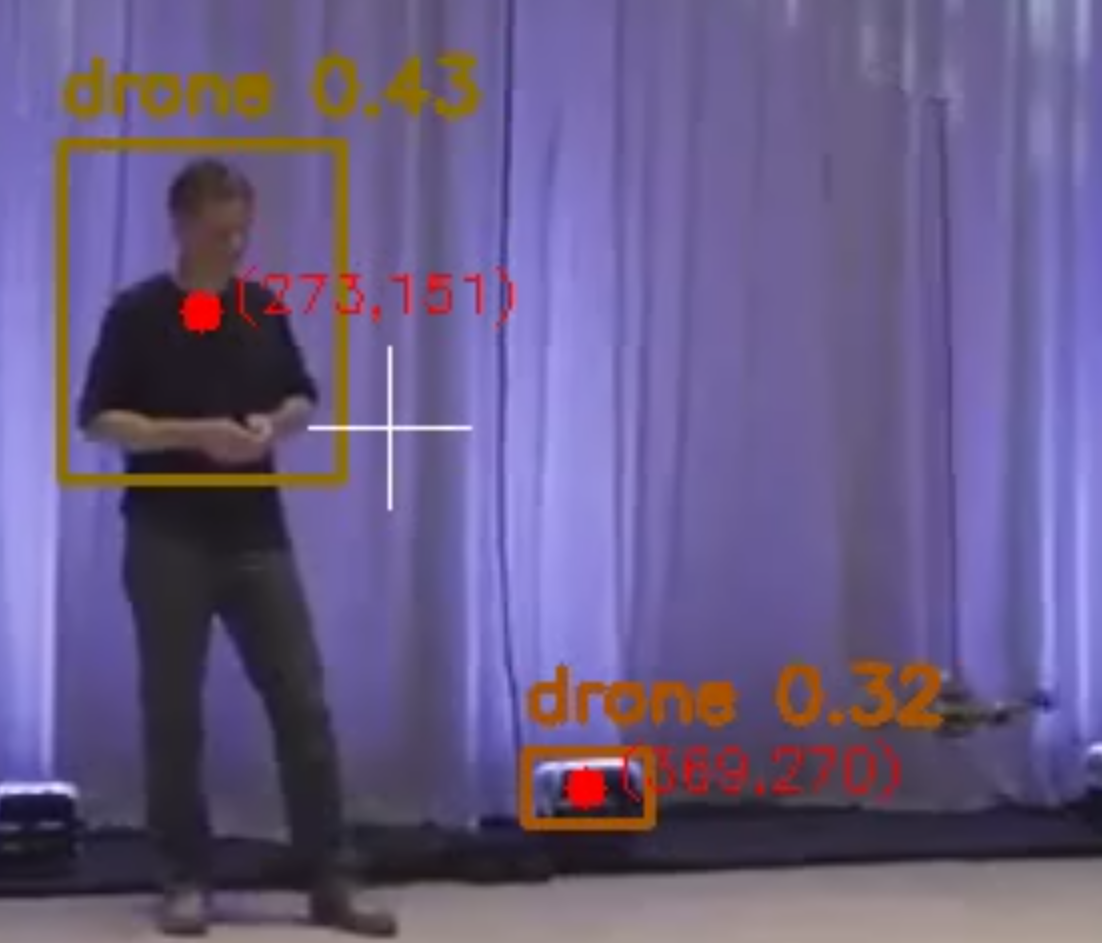
\includegraphics[width=\textwidth]{Figures/Andreas/YOLO/TED_FP_PERSON.png}
        \caption{False positive detection on a person}
        \label{fig:ted_fp_person}
    \end{subfigure}
    \vspace{0.5em}
    \begin{subfigure}[b]{0.6\textwidth}
        \centering
        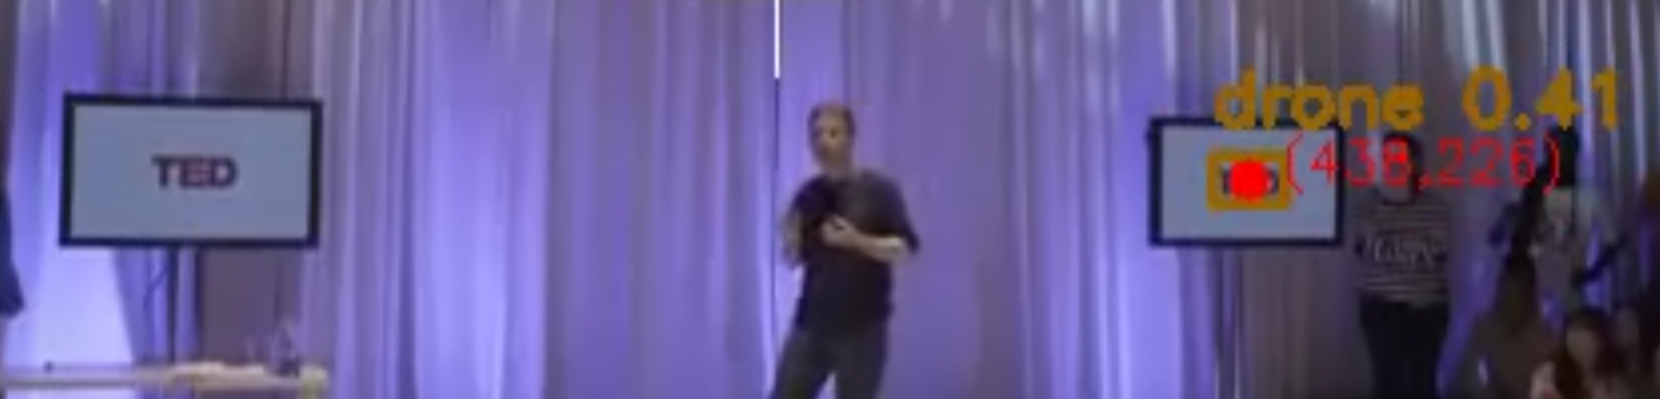
\includegraphics[width=\textwidth]{Figures/Andreas/YOLO/TED_FP.png}
        \caption{False positive detection}
        \label{fig:ted_fp}
    \end{subfigure}
    \caption[TED talk detection examples]{Example detections from the Raffaello D'Andrea TED talk, illustrating false positive detections in a cluttered dark indoor environment (\cite{dandrea2016}).}
    \label{fig:ted_detections}
\end{figure}

The YOLO detection running on the RPI was succesfull in identifying the drone flown in the lab (fig: \ref{fig:Live-lab-test}). The pixel coordinates of the center of the box detection was also successfully sent over via MQTT to the Arduino Nano in the system. 

\begin{figure}[H]
    \centering
    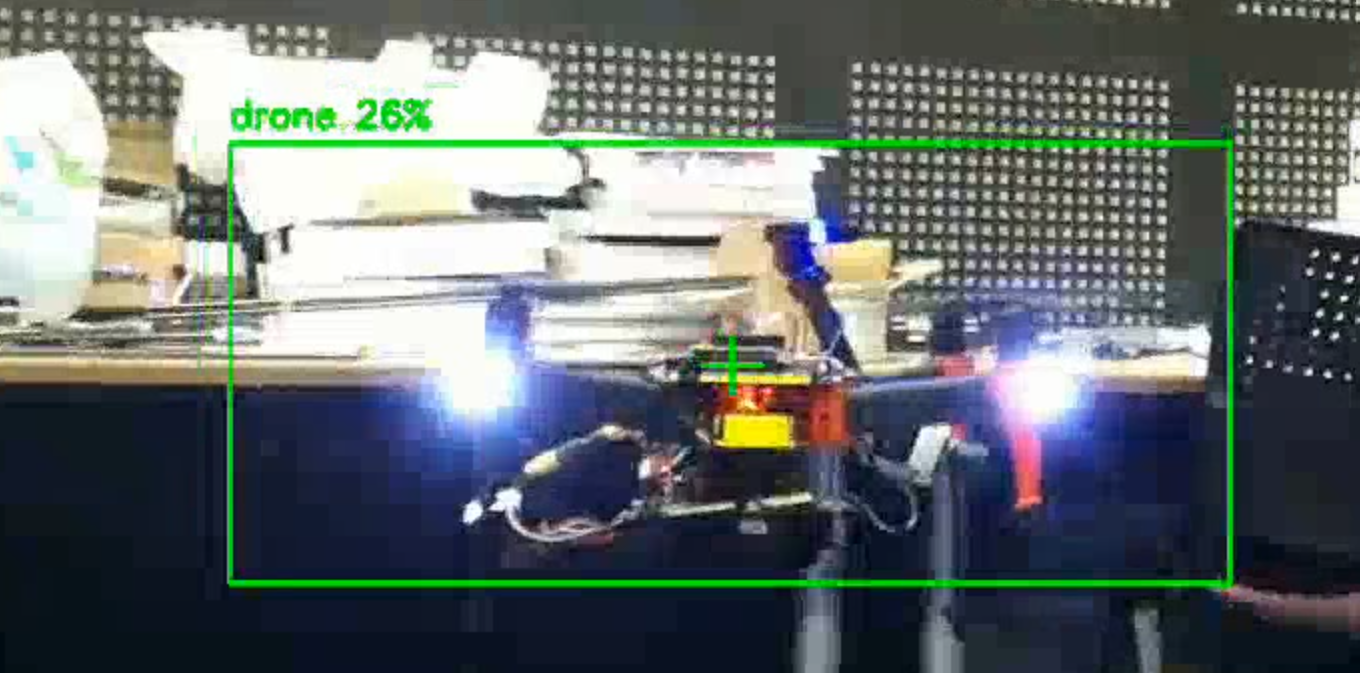
\includegraphics[width=0.5\linewidth]{Figures/Andreas/YOLO/Drone_live_lab.png}
    \caption[YOLO result live test]{Screenshot from the YOLO detection in the live lab test}
    \label{fig:Live-lab-test}
\end{figure}

It should be noted that the live laboratory test was intentionally limited 
in scope. Since the camera tracking functionality was not completed, a 
comprehensive evaluation of the visual detection subsystem was not 
prioritised at this stage. The test was further constrained by the 
laboratory environment itself: the drone could only be flown in close 
proximity to the camera platform due to safety restrictions, the indoor 
setting does not represent the outdoor backgrounds the model was trained 
on, and the drone model available in the laboratory has an irregular 
appearance that differs from the consumer quadcopters dominant in the 
training dataset (\cite{DroneDatasetFinal}). These factors mean the live 
test should be interpreted as a basic proof-of-concept demonstration 
that the inference pipeline functions on the Raspberry Pi hardware, 
rather than a rigorous evaluation of detection performance.


\section{Sound classification result}

The Convolutional Neural Network (CNN) was assessed with TensorFlow’s built-in evaluation function(Figure 4.7.1). On the public dataset the CNN attained an accuracy of 0.80, whereas on the microphone‑array recordings it reached 0.99 accuracy. Moreover, when the microphone‑array data were supplied directly to the trained CNN, the model achieved a perfect score of 49/49 correctly classified instances (Figure 4.7.3a).


\begin{figure}[H]
    \centering
    \begin{subfigure}[a]{0.48\textwidth}
        \centering
        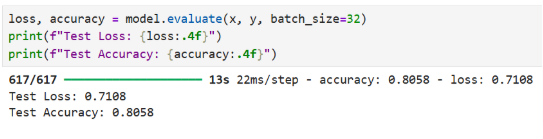
\includegraphics[width=0.95\linewidth]{Figures/Brage/CNNTestPublicData.PNG}
        \caption{CNN evaluation with public datasett(\cite{AudioDatasett})}
        \label{fig:placeholder}
    \end{subfigure}
    \begin{subfigure}[b]{0.48\textwidth}
        \centering
        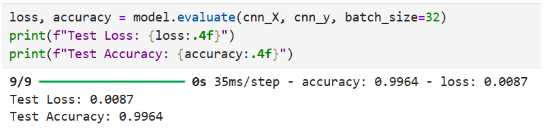
\includegraphics[width=0.95\linewidth]{Figures/Brage/CNNTestMicData.PNG}
        \caption{CNN evaluation with data form microphone array}
        \label{fig:placeholder}
    \end{subfigure}
    \caption{CNN model Tensorflow.evaluate tests}
    \label{fig:placeholder}
\end{figure}

The accumulative model was evaluated in two ways: by using scikit-learn’s k-fold cross-validation (k=5) and by feeding dedicated test sets of sound data directly to the classifier.Using the 5-fold cross-validation, the model achieved a mean accuracy of 0.90(Figure 4.6.2). 

\begin{figure}[H]
    \centering
    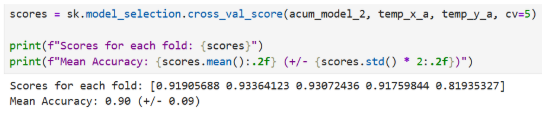
\includegraphics[width=0.9\linewidth]{Figures/Brage/AccumTestCroVal.PNG}
    \caption{Testing of the accumulative model with scikit-learn k-fold cross-validation (k=5)}
    \label{fig:placeholder}
\end{figure}

In contrast when the model was tested with data from the on-board microphone array, The performance collapsed: all predictions were incorrect i.e. the model behaved opposite to expectations(Figure 4.6.3a). When tested directly with a test set composed of the public dataset, which formed the majority of the evaluation data, the accumulative model produced results comparable to those of the CNN model(Figure 4.6.3b).


\begin{figure}[H]
    \centering
    \begin{subfigure}[a]{0.48\textwidth}
        \centering
        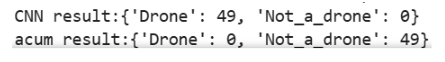
\includegraphics[width=0.9\linewidth]{Figures/Brage/MlTestMicData.PNG}
        \caption{Direct Testing of the CNN model and Accumulative model with data from microphone array}
        \label{fig:placeholder}
    \end{subfigure}
    \begin{subfigure}[b]{0.48\textwidth}
        \centering
        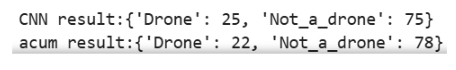
\includegraphics[width=0.9\linewidth]{Figures/Brage/MlTestPublicData.PNG}
        \caption{Direct Testing of the CNN model and Accumulative model with data from public datasett(\cite{AudioDatasett})}
        \label{fig:placeholder}
    \end{subfigure}
    \caption{Direct Testing of the CNN model and Accumulative model}
    \label{fig:placeholder}
\end{figure}

During a live-system test the machine-learning models performed identically to the isolated environment evaluations. The CNN model produced no false-positive or false-negative predictions, whereas the accumulative model consistently outputted the negative class.

The experiment was repeated five times with a drone in flight. In all tests the same outcome was observed, except for a single outlier: the accumulative model detected the drone once out of 30 total prediction iterations(Figure 4.6.4b).

\begin{figure}[H]
    \centering
    \begin{subfigure}[a]{0.48\textwidth}
        \centering
        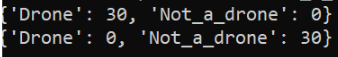
\includegraphics[width=0.85\linewidth]{Figures/Brage/LiveTestStandard.PNG}
        \caption{Standard Machine learning result from live test, upper CNN model, bottom Accumulative model}
        \label{fig:placeholder}
    \end{subfigure}
     \begin{subfigure}[b]{0.48\textwidth}
        \centering
        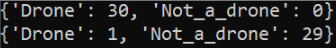
\includegraphics[width=0.85\linewidth]{Figures/Brage/LiveTestOutlier.PNG}
        \caption{Outlier Machine learning result from live test, upper CNN model, bottom Accumulative model}
        \label{fig:placeholder}
    \end{subfigure}
    \caption{Machine learning result from live test}
    \label{fig:placeholder}
\end{figure}

\section{WebServer result}
The webserver code was validated through unit testing using the jest library.The server currently runs at http://localhost:3000 and is not running on a permanent domain. It employs Socket.IO to establish a unidirectional connection with the main Python script that controls the system.
\begin{figure}
    \centering
    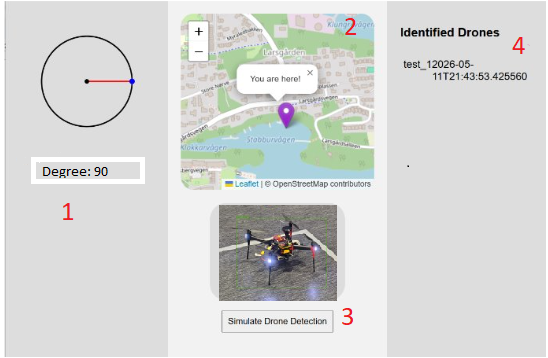
\includegraphics[width=0.75\linewidth]{Figures/Brage/GuiBuildExplain.png}
    \caption{Final build of GUI}
    \label{fig:placeholder}
\end{figure}

Figure 4.7.1 presents the final graphical user interface (GUI). Panel 1 displays a polar diagram with the azimuth degree at which a drone is detected. Panel 2 is an OpenStreetMap view with a marker for the user’s current location. Although the architecture can support drone‑position overlays, the present implementation cannot plot them because distance estimation is not yet available. Panel 3 streams the live camera feed and highlights objects that are recognised as drones. Panel 4 is intended to list identified drones; however, this feature remains under‑developed and currently provides only minimal information.

\subsection{Project Management}
The development process was initially planned according to the Scrum framework .Because team members had varied work schedules and focus on different parts , the actual workflow evolved into a Scrum‑inspired hybrid rather than a strict implementation of Scrum. Mid‑sprint review meetings were held whenever the majority of the team was available. Bi‑weekly sprint‑retrospective meetings were retained, involving the product owner, the project supervisors and the development team.

\clearpage


\chapter{Discussion}
% placeholder, will be updated soon

\section{STM32 based MCUs used in the project}
\label{sec:stm32_models_reasoning}
The first model of the STM32 used in the project, was the \href{https://www.st.com/en/microcontrollers-microprocessors/stm32f446.html}{STM32F446}, in combination with the \href{https://www.st.com/en/evaluation-tools/x-nucleo-cca02m2.html}{CCA02M2} extantion board.\\ The MCU was programmed to accquire the data signal from the microphones through the SAI peripheral, where the microphones were pairwaise connected to the same line, sending the data either at the rising edge of the common clock signal, or the falling edge. As presented in the section covering the SAI aquisition test, the signal sent by the MCU to the python based receiver, was contested to such a degree, that the DOA estimation wasn't able to reliably estimate the DOA of the strongest sound source. The group has also tried to implement the SPI in combination with I2C, to acquire the sound before the change in the MCU, which unfortunetly did not result in the correct sound acquisition. \\ % maybe add some more about that

This has led to change in the MCU to a \href{https://www.st.com/en/microcontrollers-microprocessors/stm32h743-753.html}{STM32H753} platform, which has a dedicated mode in the SAI peripheral for acquisition of the interleaved PDM signal from up to 6 microphones using the same SAI block. After many changes to the SAI, DMA configurations, and the main program for the MCU, the change in the signal sent to the receiver was non. The signal was still very highly correlated between the microphones on the same line, and the DOA estimation was random. The student has tried to use the \href{https://www.st.com/resource/en/user_manual/um2372-stm32cube-pdm2pcm-software-library-for-the-stm32f4f7h7-series-stmicroelectronics.pdf}{PDM2PCM} library, both by de-interleaving the signal before the PDM values were converted to the PCM format, and right after the conversion aswell. The resulting signal aqcuired by the receiver, was still unusable from the DOA estimation perspective, which has led to the chagne of the peripheral from SAI to DFSDM.\\

Originally the STM32H753 was meant to be used for implementation of the DFSDM, since it has a dedicated DFSDM module, but during the testing process of the MCU, the connectors for the USB were damaged, which has forced the student to change the MCU, to still be able to send the desired data load from the MCU to the receiver script.\\

The last MCU tested for audio acquisition in the project, and also applied in the final project design is the \href{https://www.st.com/en/microcontrollers-microprocessors/stm32f413-423.html}{STM32F413}. This MCU has two dedicated DFSDM modules, which also allow for higher number of microphones impemented in the system . This could be beneficiary if the system would be used to estimate the DOA in the three dimentional space. 
The MCU was also connected to the CCA02M2 extantion board, just as the two previous MCUs, to simplifie the signal acquisition from the micropohones. The main difference howerver, was that each microphone data pin was directly connected to its channel input at the MCU. In this way, the PDM values did not have to be manually de-interleaved before the PDM to PCM conversion. Since the MCU was to convert the PDM values into the PCM values inside of the DFSDM peripheral, there was no further need of applying the PDM2PCM library in the main code, which has simplified the debugging process. The MCU was the only one to correctly acquire the microphone signal, and managed to send it to the receiver so that the DOA could be correctly carried out. This has conviced the group to implement this MCU in the final design. 


% mention that the usb pins were damaged during the soldering process to defend the change to the f413
\section{Troubleshooting of the sound acquisition process based on the SAI}
\label{sec:troubleshooting_sound_acquisition}

The troubleshooting that ultimatley led to the change of the peripheral, was conducted due to the data signal from the microphones producing seamingly random DOA estimat of the strongest sound source. The system for audio acquisition, was then based on the STM32H753, which was connected to the CCA02M2 extantion board responsible for supplying, and handling the data from the microphones. The MCU SAI peripheral was generating the common clock signal for the microphones in the frequency of around 2 Mhz. The data pins from the microphones were connected pairwise on the data line, so that one microphone would send the data when the common clock signal was on the rising edge, and the other one, when the clock signal was on the falling edge. To achieve that, one of the microphones L/R pin had to be connected to the GND, while the other had to be connected to the 3.3V. \\

The first in the system to be controlled, was the above-mentioned L/R pin voltage levels. If both of the microphones in the pair would have the same voltage level on these pins, the data signal might be sent at the same moment, mixing the signals.\\
\newpage
The next to be controlled, was the code responsible for initialization of the filter handlers and their configuration. The code itself has changed several times during the troubleshooting proces, but one of the first initialization methods applied, can be accesed in Code~\ref{lst:filter_handler_config}.  

\begin{lstlisting}[style=cstyle, caption={Initialization of the filter handlers and their config}, label={lst:filter_handler_config}]
for (uint32_t index = 0; index < 2; index++)
	    {
	        PDM_FilterHandler[index].bit_order = PDM_FILTER_BIT_ORDER_MSB;
	        PDM_FilterHandler[index].endianness = PDM_FILTER_ENDIANNESS_BE;
	        PDM_FilterHandler[index].high_pass_tap = 1073741824; //2104533974
	        PDM_FilterHandler[index].in_ptr_channels = 2;
	        PDM_FilterHandler[index].out_ptr_channels = 2;

	        PDM_Filter_Init(&PDM_FilterHandler[index]);

	        PDM_FilterConfig[index].output_samples_number = 16;
	        PDM_FilterConfig[index].mic_gain = 0;
	        PDM_FilterConfig[index].decimation_factor = PDM_FILTER_DEC_FACTOR_64;

	        PDM_Filter_setConfig(&PDM_FilterHandler[index], &PDM_FilterConfig[index]);
	    }
\end{lstlisting}

The filter handlers were first planned to use a buffer per data line, that holds the interleaved values in the 8-bit format per microphone value, where the data from one microphone was to be indexed at the odd number, and the next one at the even number. Hence the \textbf{in\_ptr\_channels} and \textbf{out\_ptr\_channels} were both set to two, so that the handler would then return the PCM values using the same indexing logic, as for the input. During the testing however, it turned out that the values are very highly correlated, sugesting that the deinterleave of the values was not correct or simply lacking, which was later proven by lack of the above-mentioned function in the library, as seen in Figure~\ref{fig:fuckpdm2pcm}. 
 

\begin{figure}[h]
    \centering
    
\includegraphics[width=0.5\linewidth]{Figures/pdm2pcmFUCKYOU.png}
    \caption{Lack of implementation of the deinterleave function in the PDM2PCM library. Source:\cite{st_um2372_pdm2pcm}}
    \label{fig:fuckpdm2pcm}
\end{figure}

The lack of dedicated deinterleave function, has forced the student to use selfmade function, which has also changed during the testing process, but one of the implementations can be seen in Code~\ref{lst:pdm_deinterleave_2_mics}.

\begin{lstlisting}[style=cstyle, caption={Method used to deinterleave two mics from one buffer at a time}, label={lst:pdm_deinterleave_2_mics}]
void PDM_Deinterleave_2_mics(const uint8_t *src, uint8_t *mic1, uint8_t *mic2,uint16_t len)
		{
			for (uint16_t i = 0; i < len; i += 2)
			{
				mic1[i/2] = ((uint8_t*)src)[i];
				mic2[i/2] = ((uint8_t*)src)[i + 1];
			}
		}
\end{lstlisting}
\newpage
After applying the above-mentioned method, the in\_ptr\_channel and out\_ptr\_channel were set to be equal one, as the buffers sent to the \textbf{PDM\_Filter} method were only expected to hold the data from one microphone, as seen in Code~\ref{lst:application_pdm_filter}.

\begin{lstlisting}[style=cstyle, caption={Application of the PDM\_Filter method}, label={lst:application_pdm_filter}]
 PDM_Filter(pdm_mic1, pcm_mic1, &PDM1_filter_handler);
 PDM_Filter(pdm_mic2, pcm_mic2, &PDM2_filter_handler);
 PDM_Filter(pdm_mic3, pcm_mic3, &PDM3_filter_handler);
 PDM_Filter(pdm_mic4, pcm_mic4, &PDM4_filter_handler);
\end{lstlisting}

Despite the application of several of deinterleave functions, and other changes to the code, the values sent by the MCU were still unable to produce a meaningfull DOA estimation. The correlation matrix from the results section, suggests that there was higher then expected correlation between the data signals on the same data line, which seams to caused by the incorrect channel separation or data leakage between the microphones. The easiest way to solve the issue at that time, seamed to be the change of the peripheral used by the MCU, which resulted in correct data signal acquistion and later quite precise DOA estimation.   
%
\section{Number of microphones used in the system}
From the begining of the design process, it was planned to use four microphones to accquire the acoustic signal around the tower, to later estimate the DOA of the incoming drone in a two dimentional space. The results prove that it is possible, and the estimated DOA is also quite accurate. It was however considered to expand the number of microphones used in the system, to increase the accuracy of DOA estimation and possibly add some redundency in the system, in case of failure of several microphones. It was also considered to use several independent units equiped with microphone arrays covering 360$\circ$ around each unit, which would be in constant communication with each other and the main tower. In this way the system would also be capable of estimating the distance of the drone and the main tower, by comparing the distances between units and their TDOAs. It is just a theroetical assumption that would have to be furtherly tested and reaserched on.      

\section{Change from UART to USB CDC}
In the early stages of the project, the UART was used to send the PCM data from the MCU to the receiver script. However during testing of the sound acquisition module, it was found that the payload per second, that the UART is capable of transmitting, is too low for then used desired sampling frequency. With four microphones, a 16-bit PCM samples with addition of a start and a stop bit per byte, and a desired sampling frequency of approx. 20 kHz, the recquired data payload would be as seen in Equation~\ref{eq:payload_no_overhead}.  

\begin{equation}
\label{eq:payload_no_overhead}
    payload = 20kHz \cdot 4 \cdot 2 \cdot 10 = 1.6Mbit/s
\end{equation}
\newpage
To acquire the desired 1.6Mbit/s of data, the baudrate of atleast 1.6 MBaud would be necessary. 
Accoridng to \cite{analog_uart}, the highest baudrate found in their table is 1.5 MBaud,  which would not satisfy the desired data transmition per second. It was assumed that maybe a higher baudrate could be applied, by the student was afraid that the data transmittion would be unstable, resulting in the loss of data. 
The later applied USB CDC FS, was able to transmitt the data in the speed of 12 Mbit/s as described in the theory section covering the USB, and as seen in Figure~\ref{fig:usb_fs}, which was the main why the USB CDC FS was applied in the final project.  

\begin{figure}[h]
    \centering
    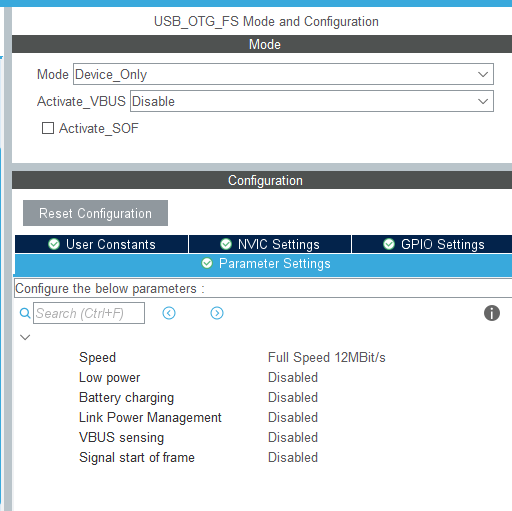
\includegraphics[width=0.5\linewidth]{Figures/speed_usb.png}
    \caption{Speed of the USB FS}
    \label{fig:usb_fs}
\end{figure}


%\section{sound pressure level measurements should have been conducted}

\section{Duration of the sound recording, and additional overhead in the system}
Duration of the sound recording varied, depending on which part of the system was tested and at which stage the test was conducted. During the early stages of the sound acquiering testig, when it was necessary to verify if the system is at all able to estiamte the DOA, the duration of 4 seconds per recording was used. In the later stages, when the DOA was proven to produce an accurate estimate, the duration has varied from 0.5s to around 1s per recording. At that stage the recordings of 0.5s durations were not reliable enough for the DOA to produce a correct estimate, so the group has sticked to the 1s durations for other tests aswell. After some consideration, the main reason for the unrealiable DOA estiamation using the 0.5s recording, seams to be the type of sound tested, which was the human speach and clapping sounds. This made it possible for the system to not catch the produced sound during the recording period.\\
\newpage
During the final test, when the recording period was set to 1s, the system has expirienced a significant lag between each DOA estimation, of around 3.4s per iteration. After the figure generating modules were deactivated in the system, the lag between each iteration was approx 1.26s, which proves that the main reason for the lag in the system was the generation and saving of DOA estimates, and Mel-spectrogram for each recording. This also proves that the easiest way to produce the DOA visualization, is simply by sending new estimated azimuth to the already initialized GUI.\\

\section{Wires used for the current design}
During the testing process the design used the following type of wires: \href{https://no.rs-online.com/web/p/breadboard-jumper-wires/7916454?cm_mmc=NO-PLA-DS3A-_-google-_-CSS_NO_EN_Pmax_Test-_--_-7916454&matchtype=&&gclsrc=aw.ds&gad_source=1&gad_campaignid=20298225819&gbraid=0AAAAADkeWNNR65FpdoBu5Vw5TPO3sZJXO&gclid=CjwKCAjw8arQBhB9EiwAfIKdQmniRsQJ3BquaxlQT0Hdzn6rzL6tpD5bGd_lQR6NpS9tRgIWoZC9VxoCEAQQAvD_BwE}{wire jumpers}. The wires are far from being perfect for high frequency data transmittion, due to lack of any additional protection against the EMI. In the final product, the transmittion wires would be changed to the F/FTP cabels, which according to \cite{linkpp_stp_cable_2025} use the foil shield per wire pair, and an additional foil shielding for the whole cable, which seams to be enough for the enviroment the product would find it self in.\\

Alternatively the data could also be transfered by the fiber-optic cables, which by design are completly resistant to the EMI, as they instead of carying the electrical signal, they carry the "light signal". However the eventual use of the fiber-optic cable, would introduce additional complexity in the electronical desing in form of an aditional fiber optic converter, which increases the total cost per unit.     


\section{Redesign of the upper PCB}
The final version of the PCB as demonstrated in the method section, has eveloved from another version seen in Figure~\ref{fig:the_old_upper_pcb}. The previous design, was meant to include the \href{https://no.rs-online.com/web/p/power-motor-robotics-development-tools/1360748}{Stepper 2 Click} motor controller based on the \href{https://www.pololu.com/file/0j450/a4988_dmos_microstepping_driver_with_translator.pdf}{A4988} chip to control the stepper motors. 

\begin{figure}[h]
    \centering
    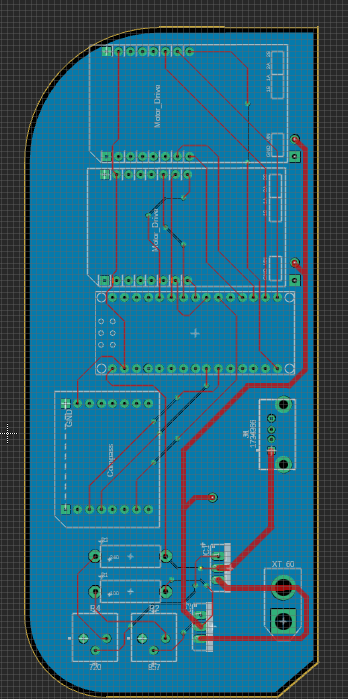
\includegraphics[width=0.25\linewidth, angle=-90]{Figures/old_upper_design.png}
    \caption[The old upper PCB design]{The old upper PCB design, using the A4988 based motor controller}
    \label{fig:the_old_upper_pcb}
\end{figure}
\newpage
The main reason for the change of the motor controller to the L6205N, was that during the PCB testing the controller has never managed to drive the stepper motor used in the design. The controller itself was rapidly heating up when being applied the signal voltage, which might suggest the internal overcurrent protection system was shuting down the control circuit. After the troubleshooting of the system, the easiest solution to that problem, seamed to be the application of the L6205N, which would be protected by the protection system applied in the LM338 voltage regulator. 

\section{Use of The bottom PCB as a substitute of the CCA02M2 extation board}
The CCA02M2 which was used in the early stages of the project, was meant to be replaced by the bottom PCB design shown in the method section. The reason for that was the reduction of the number of wires used in the system, as they were assumed to be more exposed to the EMI, then the PCB itself. The other reason was the design of the tower, which would only allow the CCA02M2 to be mounted on top of the STM32, if the walls of the bottom tower part were made even taller, to make sure that the gears from the upper part would not get in contact with the wires, or other sticking parts from the extantion board.


\section{Distance detection of the sound source}
The system currently does not allow for the distance detetion of the incoming drone solely based on the acoustic data. In the current design the distance to the drone may only be estimated based on the camera feed.

\section{Prediction of the future DOA based on the rate of change - NOT DONE}

.............

\section{Use of threads in the program}
The current program design for sound acquistion and processing, as seen in the flowcharts included in the methods section, is sequenctional. This forces the program to execute each consecutive step such as MFCC extraction and the DOA estimation, before the new sound could be recorded and processed. This creates the additional lag and inaccuracy in the DOA estimation, as the estimated DOA represents the position of the drone at start of the iteration, and not necessarily the drone position after the full processing pipeline has finished.\\

A threaded design could reduce this problem by allowing one thread to continously receive or buffer the new audio samples, while another thread would be processing already acquired sound signal. A possible application would be a producer-consumer structrue, where the audio receiver would act as the producer, which continously reads the incoming PCM samples from the STM32 MCU, and would place the complete audio frames into a shared queue. The part of the program responsible for the signal processong, would then act as the consumer, taking the oldest available audio frame from the queue, and would perform the necessary conversions and processing. In this way the new data could be acquired, while the processing modules would be processing the previously sampled data. As a result the created gaps between the readings could be reduced. Based on explenation from \cite{anderson_producer_consumer_python}. 

\section{Use of beta value for PHAT - NOT DONE}
The PHAT weighiting............

\section{frequency mask for PHAT weighting}
The frequency mask used in the PHAT weighting is currently excluding the signal values otside of the desired frequency band of between 80 to 6000 Hz. The upper limit chosen arbitrary during the testing stage, as the students lacked the reliable infromation on which frequency bands were present in the sound produced by drone available in the laboratory. The lower limit of 80 Hz, was applied to reduce the eventual influence of the power lines, which operate at the frequency level of 50 Hz. After the final test, it may be concluded that the band interval may be reduced from 6000 Hz, to less then 4000 Hz to furtherly reduce the influence of the noisy frequnecy bands. This may however have quite negative influence onto the detection system, if the drone to be detected would produce acoustic signal, where most of energy would be found in the high frequency bands.  









%For the end product, the bottom PCB seen in Figure~\ref{fig:3d_model_bottom_pcb} would be applied instead of the CCA02M2 board.
%\section{The reason for the applied distance between the microphones and the platforms center}
%\section{Use of the preemphesized signal for mfcc and the original signal for log-mel}
% i forgot to change the signal type, when i have added the preemphesis :P . 
%\section{Use of different mfcc coeffs}
%\section{Use of a 32-bit word as the DMA buffer}
%\section{The reason why The bottom PCB was not included in the final project}
%\section{Idea of using the rotory microphone system}
%\section{Reduction of the frequency mask interval for the phat weighting filter}
%, but based on the frequency bands present during the test, the band-pass could be safely reduced from 6000 Hz, to maybe even 1000 Hz.
% mics go around


\section{Raspberry PI and YOLO performance}

The hardware benchmarking results demonstrate that a Raspberry Pi 5 running YOLOv8n inference purely on the CPU is insufficient for real-time drone tracking, while the addition of the Hailo AI accelerator brings performance well within an acceptable operational range. (\ref{fig:Interference_comp}) At an average inference time of 235.6ms, the CPU-only pipeline achieves approximately 4.25 frames per second, which is too slow for smooth tracking, which would cause problems in cases of rapid drone movement. (\ref{fig:Interference_comp}) The Hailo-accelerated pipeline, by contrast, achieves an average inference time of 9.2ms, corresponding to approximately 108 frames per second, far exceeding the minimum threshold typically associated with real-time object tracking. (\ref{fig:Interference_comp})

 \vspace{1em}
 
CPU usage and temperature also carry implications for deployement. In the CPU-only configuration, the CPU usage averaged at 92.5\%, leaving little room for other system processes. (\ref{fig:cpu_usage_comparison}) By contrast, by using the HAILO chip to offload the interference, the CPU usage declined to 29.7\% giving the system more headroom for other processes and applications, as well as potential future expansions of the program. (\ref{fig:cpu_usage_comparison}) The CPU temperature results reinforce this picture: the CPU-only configuration showed a steadily rising temperature that stabilised around 73°C, a level that risks thermal throttling in enclosed or low-airflow enclosures typical of embedded systems.(\ref{fig:cpu_temp_comparison}) The Hailo configuration maintained a stable 54°C with no upward trend, suggesting reliable sustained operation. (\ref{fig:cpu_temp_comparison}) 

 \vspace{1em}
 
The RAM overhead introduced by the Hailo pipeline, approximately 140 MB higher on average than the CPU-only configuration, is the one metric that marginally favours the CPU-only approach. (\ref{fig:RAM Usage}) However, given the 8GB RAM available on the Raspberry Pi 5, this difference is negligible in practice and does not affect the overall conclusion. On the other hand, the RAM usage in both configurations utilised close to 4GB of RAM (\ref{fig:RAM Usage}), indicating that 8GB of RAM is the minimum amount of system RAM to be used for drone detection. 

\vspace{1em}

It should also be noted that the model quantization during the ONNX 
to HEF conversion was performed using randomly generated calibration 
data via the \texttt{--use-random-calib-set} flag, rather than a 
representative set of real drone images. Proper quantization 
calibration using images from the training dataset would allow the 
compiler to derive more accurate activation statistics, and would 
likely reduce the accuracy loss introduced by the 32-bit to 8-bit 
weight quantization, potentially improving detection confidence 
and bounding box precision during inference on the Hailo hardware.

 \vspace{1em}

 Taken together, these results suggest that for a low-cost real-time drone detection and tracking system, the minimum viable hardware configuration is a Raspberry Pi 5 paired with a Hailo AI accelerator. The CPU-only Raspberry Pi 5, despite being a capable single-board computer, cannot sustain the inference throughput required for reliable tracking. The Hailo chip is a relatively low-cost dedicated neural network accelerator, and its inclusion transforms an otherwise insufficient platform into one capable of smooth real-time inference with substantial CPU headroom remaining for system integration
 
  \vspace{1em}
  
The camera tracking system was not completed on time due to issues with controlling the stepper motor, with the most likely culprit being the voltage given on the 10V rail, which was measured to be at 12V. The exact reason for this is unclear, altough mostly likely it is due to a faulty component and not the design itself. This most likely caused the voltage regulator to overheat, as well as the stepper motors to jitter. However, The stepper motors still moved enough to confirm that the Pan and Tilt function worked as designed.

In most camera sensor solutions for drone detection, higher quality cameras with optical zoom are often optimized, as that would increase the range of the drone detection system. 



\section{Drone detection performance}

The results demonstrate that the YOLOv8n achieved a stronger performance on the drone detection dataset (\cite{DroneDatasetFinal}) in comparison to the MobileNet V1 model used in the original paper. The YOLOv8n model avhieved a mAP@50 of 0.832, compared to the 0.533 of the highest performing MobileNet V1 model (\cite{DroneDatasetFinal}). The peak F1 score (\ref{tab:yolo_detection_performance}) of 0.81 at a confidence threshold of 0.571 exceeds the original papers maximum of 0.602. Both models were trained and tested on the same datasets, with the difference being attributed to improvements within object detection model architecture.


MobileNet V1 was originally proposed by \cite{howard2017mobilenets} in 2017 as a lightweight architecture designed primarily for mobile and embedded applications (\cite{howard2017mobilenets}). The SSD detection framework it was paired with predates many advances which have now become standard in object detection models.YOLOv8, released by Ultralytics in 2023, incorporates a CSPDarknet-based backbone, a Feature Pyramid Network combined with a Path Aggregation Network in the neck for multi-scale feature fusion, and an anchor-free decoupled detection head that independently handles classification and bounding box regression — removing the need for predefined anchor templates and reducing post-processing overhead (\cite{terven2023comprehensive, jocher2023yolov8}). These advance,s as well as a more refined training pipeline, represent the progress made within the field of object detection. The results of the original papers performance in comparison to the one presented in this study is reflective of the generational gap within object detection algorithms.   

 \vspace{1em}

Another possible contribution to the improved results is the higher input resolution used in this study, 640x640, in comparison to the original papers 300x300 (\cite{DroneDatasetFinal}). Since the dataset contains a high proportion of images where the drone appears small, a higher resolution is advantagous since it preserves more of the spatial details. The augmentation strategy, including mosaic augmentation, scale jitter, and rotation, is well-suited to the dataset's variability in drone size, viewing angle, and background environment.

Selection of the dataset was found to be the most critical factor across the training process, as multiple models were trained on different datasets before arriving at the final configuration. The dataset used was selected because it produced the model with the fewest false positives, with the key advantage being the large number of background-only images in the validation set. These negatives actively penalise the model for spurious detections during training, encouraging greater specificity (\cite{DroneDatasetFinal}). This effect is also visible in the validation loss curves, where the classification loss showed an anomalously high scale (~16–27) compared to the training classification loss (~0.40), directly attributable to the 2,750 background-only images in the validation set penalising false detections (\ref{fig:pYolo_results}).

\vspace{1em}

The normalised confusion matrix shows that all background instances in the test set were assigned a non-zero detection at some confidence level, indicating some false positives(\ref{fig:Yolo_confusion_matrix}). At the recommended threshold of 0.571 this behaviour is well controlled, as the precision confidence curve shows high precision, low false positives, in this region. (\ref{fig:pr_curve}). 

The precision-recall curve illustrates that the model maintains near-perfect precision across a wide recall range before degrading sharply beyond approximately 0.75 recall, indicating confidence and accuracy on the majority of detections with uncertainty concentrated at harder examples. The F1-confidence curve shows a broad plateau between roughly 0.3 and 0.7 confidence, suggesting the model is not overly sensitive to the exact choice of threshold within this range, which is a practically useful property for deployment. The recall-confidence curve reveals a notable strength: at near-zero confidence threshold the model achieves a recall of 0.94, meaning it detects the vast majority of drones present in the images before any filtering is applied. For a security-oriented application such as drone detection, high recall is generally prioritised over precision, as missing a drone carries greater risk than generating a false alarm.

\vspace{1em}

The mAP@0.5 score of 0.832 indicates that the model detects drones reliably, but the mAP@0.5:0.95 score of 0.420 indicates that the predicted bounding boxes are not always tightly localised \ref{tab:yolo_detection_performance}. This difference can be attributed to the difficulty of creating precise boxes for small objects. This poses a potential challenge for drone tracking applications where an accurate position estimate is required. However, for the intended use case of keeping the drone within the camera frame, imprecise localisation may be less critical provided the detection itself is reliable. The paper does not report mAP@0.5:0.95, so a direct comparison at this stricter threshold is not possible, though it is reported here for completeness. Another solution to this could be the investment in a high quality camera with a high optical zoom, altough that would most likely increase the cost of the system significantly. 

\vspace{1em}

The false positives seen in Real-world inference testing further highlighted the dataset's influence on model behaviour. The false positives observed in the Floureon FPV video \cite{floureon2017} can most likely be attributed to the dataset lacking sufficient images of drones against darker tree backgrounds \cite{DroneDatasetFinal} (\ref{fig:video_comparison}). Similarly, in the TED talk video \cite{dandrea2016}, which features a darker indoor environment cluttered with people, the elevated false positive rate likely reflects the absence of indoor drone footage in the training data. These failure cases highlight the necessity of datasets that cover a diverse range of backgrounds and lighting conditions, and suggest that targeted data augmentation or dataset expansion in these specific scenarios could improve robustness. 

\vspace{1em}

The limited scope of the live detection test reflects the state of 
the system at the time of testing rather than a fundamental limitation 
of the approach. A more rigorous evaluation of the visual detection 
subsystem would require a different experimental setup. Future testing 
should be conducted outdoors in environments representative of the 
system's intended use case --- private property, suburban areas, 
open fields, and urban settings where unauthorised drone activity 
poses the most common threat to individuals and small organisations. 
These environments also provide the backgrounds most relevant to 
the training dataset (\cite{DroneDatasetFinal}), including open sky, 
buildings, trees, and varied terrain, which should improve detection 
reliability compared to the cluttered indoor laboratory setting 
used here. The test drone should be a standard consumer quadcopter 
of the type well-represented in the dataset, rather than the 
irregular laboratory drone used in the initial test. The standard consumer quadcopters fits more with the intended use case, as these are the drones that are more of a threat towards civilians. Detection 
performance should be evaluated at several measured distances, 
for example at 10~m, 25~m, 50~m, and 100~m intervals, to 
characterise how detection confidence and bounding box precision 
degrade with range. This would also allow a meaningful assessment 
of whether the mAP@0.50:0.95 score of 0.420 --- which indicates 
imprecise bounding box localisation on small targets --- represents 
a practical limitation for the tracking application, where only 
the centre pixel coordinate is required rather than a tight 
bounding box. Finally, a complete end-to-end test with the motor 
tracking operational would allow evaluation of the full 
coarse-to-fine pipeline: acoustic DOA orienting the camera, 
followed by YOLO-driven continuous tracking, with the latency 
and angular accuracy of each stage measured independently.

\vspace{1em}

Finally, training time was a practical bottleneck throughout this project, limiting the number of training runs and the degree to which hyperparameters could be systematically explored. The NVIDIA RTX 4050 laptop GPU, while sufficient to complete training, imposed meaningful constraints on iteration speed. It is recommended that future work utilise a more powerful GPU, as this would significantly reduce training time and allow more thorough hyperparameter search and experimentation.

\section{Hardware cost comparison}

A notable gap in the existing literature on vision-based drone detection is the limited reporting of hardware costs alongside detection performance metrics. Most academic work focuses on algorithm design and benchmark accuracy, with few studies providing an itemised hardware cost for their proposed systems. One exception is the RF-based system by (\cite{swinney2022lowcost}), which explicitly reports a total edge node cost of under €490 (~kr. 5,290), though at the cost of inference times of 15–28 seconds that preclude real-time tracking (\cite{swinney2022lowcost}). Commercial drone detection solutions offer substantially higher performance but at prices that are orders of magnitude greater, with EO/IR camera systems ranging from approximately €9,000 to €72,000 (~kr. 97,000–778,000) and radar-based systems from €27,000 to over €450,000 (~kr. 292,000–4,860,000) \cite{airsight2025buyersguide}.

The system proposed in this work achieves real-time drone 
detection through the combination of acoustic direction of 
arrival estimation using a four-element MEMS microphone 
array and visual detection at approximately 108 frames per 
second using the Hailo AI HAT+ accelerator 
(\ref{fig:Interference_comp}), at a total system hardware cost of 
approximately €830 (~NOK~8,503). This represents a substantial 
reduction in cost relative to both commercial alternatives 
and the performance threshold required for practical tracking 
applications, while simultaneously providing the 
complementary strengths of omnidirectional acoustic coverage 
independent of lighting conditions and real-time visual 
confirmation with precise pixel-level localisation 
(\cite{seidaliyeva2024advances, macedo2025drone}).
\vspace{1em}


The lack of hardware cost reporting in the audio-visual drone detection literature is a recurring limitation. Svanström et al. (2020), one of the most cited multi-sensor drone detection studies combining visible, thermal, and acoustic sensors, provides no hardware cost breakdown \cite{svanstrom2020realtime}. Similarly, Ding et al. (2023) describe their acoustic-optical fusion system MUTES as having "acceptable cost" without providing specific figures \cite{ding2023drone}. This makes direct cost comparison with the system proposed in this work difficult. The absence of cost reporting in academic literature likely reflects a research culture that prioritises algorithmic performance over deployment economics, despite the practical importance of cost for the widespread adoption of drone detection systems at critical infrastructure.


\section{Sensor fusion synergy}

The combination of acoustic and visual sensing employed in this project follows 
the principle of multimodal drone detection, where each sensor modality compensates 
for the limitations of the other (\cite{seidaliyeva2024advances}). This approach 
is supported by the work of Ding et al., who proposed the MUTES system combining 
a microphone array, camera, and lidar for drone detection and tracking, employing 
a coarse-to-fine localization strategy in which acoustic direction estimation 
activates and steers the optical modules toward the target 
(\cite{ding2023drone}). Their results demonstrated that sensor fusion achieves 
higher accuracy than any individual modality alone, with a 3D positioning error 
of less than 1.5\% of the detection range (\cite{ding2023drone}).

The combination of acoustic DOA estimation and visual YOLO detection in this 
project provides complementary strengths that neither sensor achieves 
independently (\cite{seidaliyeva2024advances, macedo2025drone}). The microphone 
array can detect a drone beyond the camera's field of view and provide a 
directional estimate before the drone is visible, allowing the camera platform 
to orient towards the target (\cite{ding2023drone}). The camera then provides 
visual confirmation and precise pixel-level localisation, which reduces false 
positives from the acoustic classifier (\cite{seidaliyeva2024advances}). The 
acoustic subsystem provides omnidirectional coverage independent of lighting 
conditions and without requiring line of sight (\cite{ding2023drone}), while 
the camera subsystem provides visual confirmation and precise localisation 
(\cite{seidaliyeva2024advances, macedo2025drone}).

This sensor fusion approach is particularly valuable in low-cost systems where 
neither sensor alone is sufficiently reliable (\cite{macedo2025drone}). The 
acoustic system struggles with background noise 
(\cite{macedo2025drone, seidaliyeva2024advances}), while the camera struggles 
with small, fast-moving targets at distance and produces false positives in 
cluttered environments (\cite{macedo2025drone}). Their combination addresses 
the primary failure modes of each modality 
(\cite{seidaliyeva2024advances, macedo2025drone}), and multimodal approaches 
of this kind have been shown to achieve positioning errors below 1.5\% of 
detection range (\cite{ding2023drone}), representing a significant improvement 
over single-modality systems.

\section{GUI}
The GUI was originally intended to run on a Raspberry-Pi. During the final weeks of development the device began to overheat and started smooking, prompting us to discontinue its use because it risked further damage and could delay the project further. This also meant that the initial plan to build with the possibility to interconnect several Raspberry-Pis as a microphone‑array field could not be realised.
The server was containerised with Docker to simplify updates and to maintain compatibility with a Raspberry-Pi. Since the Raspberry-Pi was ultimately not employed, the Docker‑based implementation contributed little to the final system.

\vspace{1em}

The GUI also incorporated an SSH certificate to allow GPS coordinates to be transmitted without modifying the user’s browser. However, the absence of an Internet router that could be configured for port‑forwarding prevented us from exposing the web server beyond a localhost address.

\vspace{1em}

Although the GUI includes a fully functional Open‑Stream‑Map integration for visualising drones, the current implementation cannot reliably estimate distances; consequently, it cannot place accurate markers on the map. A possible remedy would be to represent positional uncertainty, for example by displaying a line that indicates the potential trajectory of a drone, or by rendering a cone that shows angular uncertainty (see Figure 5.17.1).


\begin{figure}[H]
    \centering
    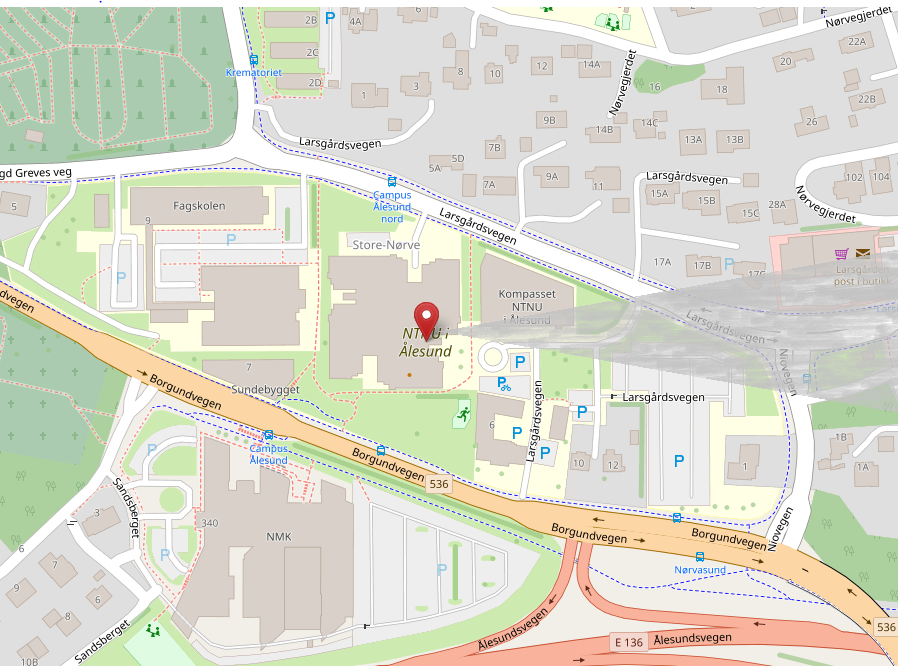
\includegraphics[width=0.5\linewidth]{Figures/Brage/mappEksempelSearchCone.png}
    \caption{Example for how a search cone showing angular uncertainty on the map could look, where the gray cone is the possible location of found drone}
    \label{fig:placeholder}
\end{figure}

Because the SSH certificate could not be deployed, the webserver does not have ample security measures. This lacking implementation represents a further development target, where the implementation of certification and stricter access-control policies should be prioritized. Nevertheless, the limited security exposure the system experiences given it is run locally means the lacking security measures does not affect the validity of the experimental results.

\section{Temp name}
As originally planned, the system was to run on two Raspberry-Pis: one dedicated to the camera and a second responsible for the web server, machine‑learning‑based sound classification, and connection to the microphone array. During integration the Raspberry-Pi designated for the primary subsystem overheated, so we migrated the live‑system test to a laptop.

This migration introduced a new problem: the newer TensorFlow release is not compatible with Windows, which forced operation in an environment with an older Python interpreter (version 3.10.20). Consequently, several dependent libraries also had to be downgraded.


The Python environment was managed with Conda to keep the package versions reproducible. Because of the version changes, The CNN loading procedure needed a minor modification: rather than loading a saved model object directly, the model architecture was initialized then was supplied the trained weight.Despite these adjustments, no functional shortcomings were observed; the system performed as expected in all preceding tests. Since the laptop exhibited no accuracy degradation and the Conda environment differs only marginally from the Raspberry-Pi setup, there is no substantial obstacle to eventually deploying the complete system on a single Raspberry-Pi. 
 

\clearpage


\chapter{Conclusions}
This project set out to develop a low-cost multimodal drone detection 
system using exclusively off-the-shelf and 3D-printed components, 
combining acoustic and visual sensing to achieve reliable detection 
without specialist hardware. The results demonstrate that this goal 
was largely achieved within the project constraints.

The acoustic subsystem successfully progressed through three 
microcontroller iterations before arriving at the STM32F413 with 
DFSDM-based PDM-to-PCM conversion as the final working 
configuration. The GCC-PHAT direction of arrival algorithm 
demonstrated accurate azimuth estimation of a live drone in 
laboratory conditions, with a full pipeline iteration time of 
approximately 1.285 seconds including sound classification. 
The CNN sound classifier achieved 99\% accuracy on microphone 
array data and performed reliably during live testing, correctly 
distinguishing drone sound from background noise in all but one 
outlier iteration out of thirty. The decision-tree accumulative 
classifier, while performing well on public dataset evaluation, 
failed to generalise to the microphone array recordings, indicating 
a domain mismatch between training data and real deployment 
conditions that warrants further investigation.

The visual detection subsystem achieved its primary objectives. 
The YOLOv8n model trained on the drone detection dataset of 
Pawełczyk and Wojtyra achieved an mAP@0.50 of 0.835 and an F1 
score of 0.81 at a confidence threshold of 0.571, outperforming 
the MobileNet V1 baseline from the original dataset paper. 
Deployed on a Raspberry Pi~5 with a Hailo AI HAT+ accelerator, 
the model achieved approximately 108 frames per second inference, 
well within the requirements for real-time tracking, at a CPU 
usage of only 29.7\% leaving substantial headroom for system 
integration. Real-time coordinate publishing over MQTT and live 
video streaming to the web-based GUI were both successfully 
demonstrated. The full closed-loop camera tracking, where motor 
movement is driven continuously by YOLO detections following the 
initial acoustic orientation, was not completed within the project 
timeframe due to issues with the motor control hardware, which 
is identified as the primary target for future development.

The complete system was realised at a total hardware cost of 
approximately NOK~8,503, representing a reduction of over an order 
of magnitude compared to entry-level commercial drone detection 
solutions, while demonstrating real-time multimodal detection 
capability. The coarse-to-fine architecture, in which acoustic 
DOA estimation narrows the search space for the visual detector, 
proved sound in principle and was partially validated through 
separate testing of each subsystem.

Future work should prioritise completing the closed-loop motor 
tracking, conducting outdoor detection performance evaluation 
at measured distances using consumer quadcopters in 
representative civilian environments, and improving the 
decision-tree classifier's generalisation to real microphone 
array data. The addition of proper quantization calibration 
using representative drone images during the Hailo HEF 
conversion process would also likely improve visual detection 
accuracy on the deployed hardware.
\clearpage


\addcontentsline{toc}{chapter}{\protect\numberline{}References}
\printbibliography[title={References}] %you may change the title in the toc here if you want
\clearpage


\chapter*{\LARGE \textbf{Appendices}}
\fancyhf{} %clear the header, it should be empty for the appendices
\renewcommand{\headrulewidth}{0pt} %no rule
\fancyfoot[C]{\thepage} %set the page numbers in the center of the footer instead 

%it is possible to set a different page numbering style for the appendix, but I personally just continued with the same page numbering as the main content as I find that more tidy
%\pagenumbering{roman}
%\setcounter{page}{1}
\addcontentsline{toc}{chapter}{\protect\numberline{}Appendices:}
\appendix


\chapter*{A - Github repository}
\addcontentsline{toc}{chapter}{\protect\numberline{}A - Github repository} 

All code and latex-files used in this document are included in the Github repositorys linked below. 


\subsection*{Github repository link, overleaf }
\begin{itemize}
    \item \url{https://github.com/BrageSolem/Acoustic-perception---Bachelor-Thesis}
\end{itemize}

\subsection*{Github repository link, code}
\begin{itemize}
    \item \url{https://github.com/BrageSolem/Acoustic-drone-detection}
\end{itemize}


\chapter{B - Supplementary Materials}
\href{Appendix files/Møtereferat.zip}{Click here to download the meeting minutes}


\end{document}
